\documentclass[
10pt,
a4paper,
openany,
svgnames,
]{book}

\usepackage[utf8]{inputenc}
\setcounter{secnumdepth}{2}
\setcounter{tocdepth}{1}

\usepackage{geometry}
\geometry{margin=1in}
\usepackage{graphicx}
\usepackage[parfill]{parskip}
\usepackage{booktabs}
\usepackage{array}
\usepackage{enumitem}
\usepackage{verbatim} 
\usepackage{subfig}
\usepackage{colortbl}

%%% HEADERS & FOOTERS
\usepackage{fancyhdr} % This should be set AFTER setting up the page geometry
\pagestyle{fancy} % options: empty , plain , fancy
\renewcommand{\headrulewidth}{1pt} % customise the layout...
\renewcommand{\footrulewidth}{1pt}
\lhead{\rightmark}\chead{}\rhead{}
\lfoot{ME 310: Mechanical Design I}\cfoot{\thepage}\rfoot{S. Akamphon}

%%% ToC (table of contents) APPEARANCE
\usepackage[numbib]{tocbibind} % Put the bibliography in the ToC
\usepackage[titles,subfigure]{tocloft} % Alter the style of the Table of Contents

\newcommand*\chem[1]{\textup{#1}}

\usepackage{newtxtext}
\usepackage[nointegrals]{wasysym}
\usepackage{newtxmath}
\usepackage{hyperref}
\hypersetup{
  colorlinks,
  citecolor=black,
  filecolor=black,
  linkcolor=blue,
  urlcolor=blue,
}

\let\openbox\relax
\usepackage{amsthm}
\usepackage{bm}
\usepackage{multirow}
\usepackage{array}
\usepackage{cleveref}
\usepackage{siunitx}

\usepackage[gobble=auto]{pythontex}

%% Chapter Heading %%%%%
\usepackage[explicit]{titlesec}

%% Drawing pics with tikz %%%
\usepackage{tikz}
\usetikzlibrary{arrows,calc,decorations,shapes,decorations.pathmorphing,patterns}
\tikzset{>=latex}
\usepackage{pgfplots}
\newcommand{\AxisRotator}[1][rotate=0]{%
    \tikz[x=0.25cm,y=0.60cm,line width=.2ex,-stealth,#1] \draw(0,0) arc (150:-150:1 and 1);%
}

\definecolor{lightblue}{RGB}{180,220,255}
\definecolor{titlepagecolor}{cmyk}{1,.60,0,.40}
\definecolor{namecolor}{cmyk}{1,.50,0,.10}
\usepackage{smartdiagram}

\titleformat{\chapter}
{\huge\bfseries}
{}{0pt}
{\begin{tikzpicture}[remember picture,overlay]
    \node[yshift=-3cm] at (current page.north west)
    {\begin{tikzpicture}[remember picture,overlay]
        \path[fill=lightblue] (0,0) rectangle (\paperwidth,3cm) ;
        \node[anchor=east,xshift=.9\paperwidth,rectangle,rounded corners=5pt,inner sep=11pt,fill=RoyalBlue]{\color{white}#1};
        \node[right, xshift=1cm]{\scalebox{4}{\Huge\thechapter}};
      \end{tikzpicture}};
  \end{tikzpicture}
}

\titleformat{name=\chapter,numberless}
{\huge\bfseries}
{}{0pt}
{\begin{tikzpicture}[remember picture,overlay]
    \node[yshift=-3cm] at (current page.north west)
    {\begin{tikzpicture}[remember picture,overlay]
        \path[fill=lightblue] (0,0) rectangle (\paperwidth,3cm) ;
        \node[anchor=east,xshift=.9\paperwidth,rectangle,rounded corners=5pt,inner sep=11pt,fill=RoyalBlue]{\color{white}#1};
      \end{tikzpicture}};
  \end{tikzpicture}
}

\titlespacing*{\chapter}{0pt}{50pt}{-10pt}

%% Section Heading %%%%%

\titleformat{\section}
{\Large\bfseries}
{}{0pt}
{\begin{tikzpicture}
    \node[fill=lightblue, rectangle, minimum height=1.5cm, minimum width=\textwidth](A){};
    \node at (A.west) [fill=RoyalBlue, anchor=west]{\color{white}\thesection\quad#1};
  \end{tikzpicture}
}
   
\titleformat{name=\section, numberless}
{\Large\bfseries}
{}{0pt}
{\begin{tikzpicture}
    \node[fill=lightblue, rectangle, minimum height=1.5cm, minimum width=\textwidth](A){};
    \node at (A.west) [fill=RoyalBlue, anchor=west]{\color{white}#1};
  \end{tikzpicture}
}

\titlespacing*{\section}{0pt}{20pt}{-10pt}

%% Subsection Heading %%%%

\titleformat{\subsection}
{\large\color{RoyalBlue}\bfseries}
{\thesubsection}{10pt}{#1}

%%% New column type
\newcolumntype{L}[1]{>{\raggedright\let\newline\\\arraybackslash\hspace{0pt}}m{#1}}
\newcolumntype{C}[1]{>{\centering\let\newline\\\arraybackslash\hspace{0pt}}m{#1}}
\newcolumntype{R}[1]{>{\raggedleft\let\newline\\\arraybackslash\hspace{0pt}}m{#1}}

%%% Example environment
\usepackage{thmtools}
\usepackage{mdframed}
\usepackage{float}
\declaretheoremstyle[
spaceabove=6pt, spacebelow=6pt,
headfont=\normalfont\bfseries,
notefont=\mdseries, notebraces={(}{)},
bodyfont=\normalfont,
postheadspace=1em,
numberwithin=chapter,
preheadhook={\begin{mdframed}[backgroundcolor=lightblue,
    innertopmargin=6pt , splittopskip=\topskip, % 
    skipbelow= 0pt, skipabove=6pt, %
    topline=false,bottomline=false,leftline=false,rightline=false] \sloppy},
  postfoothook=\end{mdframed},
headpunct={}
]{exstyle}
\declaretheoremstyle[
spaceabove=6pt, spacebelow=6pt,
headfont=\normalfont\bfseries,
notefont=\mdseries, notebraces={(}{)},
bodyfont=\normalfont,
postheadspace=1em,
preheadhook={\begin{mdframed}[backgroundcolor=lightblue,
    innertopmargin =6pt , splittopskip = \topskip, % 
    skipbelow=6pt, skipabove=0pt, %
    topline=false,bottomline=false,leftline=false,rightline=false] \sloppy},
  postfoothook=\end{mdframed},
headpunct={},
numbered=no
]{solstyle}
\declaretheorem[style=exstyle]{example}
\declaretheorem[style=solstyle]{solution}

% New list for exercises
\newlist{exercises}{enumerate}{2}
\setlist[exercises]{%
  label=\textbf{\thechapter-\arabic*}~,  % Label: Exercise C.E
  ref=\thechapter-\arabic*, % References: C.E (important!)
  align=left,               % Left align labels
  labelindent=0pt,          % No space betw. margin of list and label
  leftmargin=0pt,           % No space betw. margin of list and following lines
  itemindent=!,             % Indention of item computet automatically
}

\newcommand{\exercise}{%
\item \label{lab:\arabic{chapter}.\arabic{exercisesi}}  % Append label to item
}

\SetLabelAlign{parright}{\parbox[t]{\labelwidth}{\raggedleft#1}}

\setlist[description]{style=multiline,leftmargin=5cm,font=\bfseries,%
    align=parright}

% New decoration for screws
\tikzset{/pgf/decoration/.cd,
    head width/.initial=6pt,
    head length/.initial=1.5pt,
    thread separation/.initial=1.0pt,
    thread amplitude/.initial=0.5pt,
    screw radius/.initial=1.2pt,
}
% definition of the decoration
\pgfdeclaredecoration{screw}{initial}
{
  \state{initial}[width=\pgfkeysvalueof{/pgf/decoration/head length},%
  next state=midd]
  {
    \def\headlength{%
      \pgfkeysvalueof{/pgf/decoration/head length}%
    }
    \def\headwidth{%
      \pgfkeysvalueof{/pgf/decoration/head width}%
    }
    \def\screwradius{%
      \pgfkeysvalueof{/pgf/decoration/screw radius}%
    }
    % First line
    \pgfpathlineto{\pgfpoint{0.0pt}{\headwidth/2}}
    \pgfpathlineto{\pgfpoint{\headlength}{\headwidth/2}}
    \pgfpathlineto{\pgfpoint{\headlength}{\screwradius}}
    % Second line
    \pgfpathmoveto{\pgfpoint{0.0pt}{0.0pt}}
    \pgfpathlineto{\pgfpoint{0.0pt}{-\headwidth/2}}
    \pgfpathlineto{\pgfpoint{\headlength}{-\headwidth/2}}
    \pgfpathlineto{\pgfpoint{\headlength}{-\screwradius}}
  }
  \state{midd}[width=\pgfkeysvalueof{/pgf/decoration/thread separation}*2]
  {
    \def\threadseparation{%
      \pgfkeysvalueof{/pgf/decoration/thread separation}%
    }
    \def\threadamplitude{%
      \pgfkeysvalueof{/pgf/decoration/thread amplitude}%
    }
    \def\screwradius{%
      \pgfkeysvalueof{/pgf/decoration/screw radius}%
    }
    % First line
    \pgfpathmoveto{\pgfpoint{0pt}{\screwradius}}
    \pgfpathlineto{\pgfpoint{0.5*\threadseparation}{\screwradius+\threadamplitude}}
    \pgfpathlineto{\pgfpoint{1.0*\threadseparation}{\screwradius}}
    \pgfpathlineto{\pgfpoint{1.5*\threadseparation}{\screwradius-\threadamplitude}}
    \pgfpathlineto{\pgfpoint{2.0*\threadseparation}{\screwradius}}
    % Second line
    \pgfpathmoveto{\pgfpoint{0pt}{-\screwradius}}
    \pgfpathlineto{\pgfpoint{0.5*\threadseparation}{-\screwradius-\threadamplitude}}
    \pgfpathlineto{\pgfpoint{1.0*\threadseparation}{-\screwradius}}
    \pgfpathlineto{\pgfpoint{1.5*\threadseparation}{-\screwradius+\threadamplitude}}
    \pgfpathlineto{\pgfpoint{2.0*\threadseparation}{-\screwradius}}
    % Thread
    \pgfpathmoveto{\pgfpoint{0.5*\threadseparation}{\screwradius+\threadamplitude}}
    \pgfpathlineto{\pgfpoint{1.5*\threadseparation}{-\screwradius+\threadamplitude}}
  }
  \state{final}
  {
    \def\screwradius{%
      \pgfkeysvalueof{/pgf/decoration/screw radius}%
    }
    %\pgfpathlineto{\pgfpointdecoratedpathlast}
    \pgfpathmoveto{\pgfpoint{0pt}{\screwradius}}
    \pgfpathlineto{\pgfpoint{\screwradius/2}{0pt}}
    \pgfpathlineto{\pgfpoint{0pt}{-\screwradius}}
  }
}

%% bibliography %%%%

\usepackage[style=numeric,backend=biber]{biblatex}
\addbibresource{me310.bib}

%%% END Article customizations

%%% The "real" document content comes below...

%%%%%%%%%%%%%%%%%%%%%%%%%%%%%%%%%%%%%%%%%%%%%%%%%%%%%%%%%%%%%%%%%%%%%%%%%%%%%%%%%%%%%%%%%%%%%%%%%%%%%%%%%%%%%%%%%%%%%%%%%%%%%%%%%%%%%%%%%%%%%%%%%%%%%%%%%%%%%%%%%%%%%%%%%%%%%%

\begin{document}

\frontmatter

%\maketitle
\begin{titlepage}
  \newgeometry{top=1cm,left=1cm} %defines the geometry for the titlepage
  \pagecolor{titlepagecolor}
  \raggedright 
\includegraphics[scale=0.2]{pictures/logo-tu} \\
  \noindent
  \color{white}
  \makebox[0pt][l]{\rule{1.3\textwidth}{1pt}}
  \par
  \noindent
  \textbf{\textsf{Thammasat University}} \textcolor{namecolor}{\textsf{Faculty of Engineering}}
  \vfill
  \hspace{1cm}
  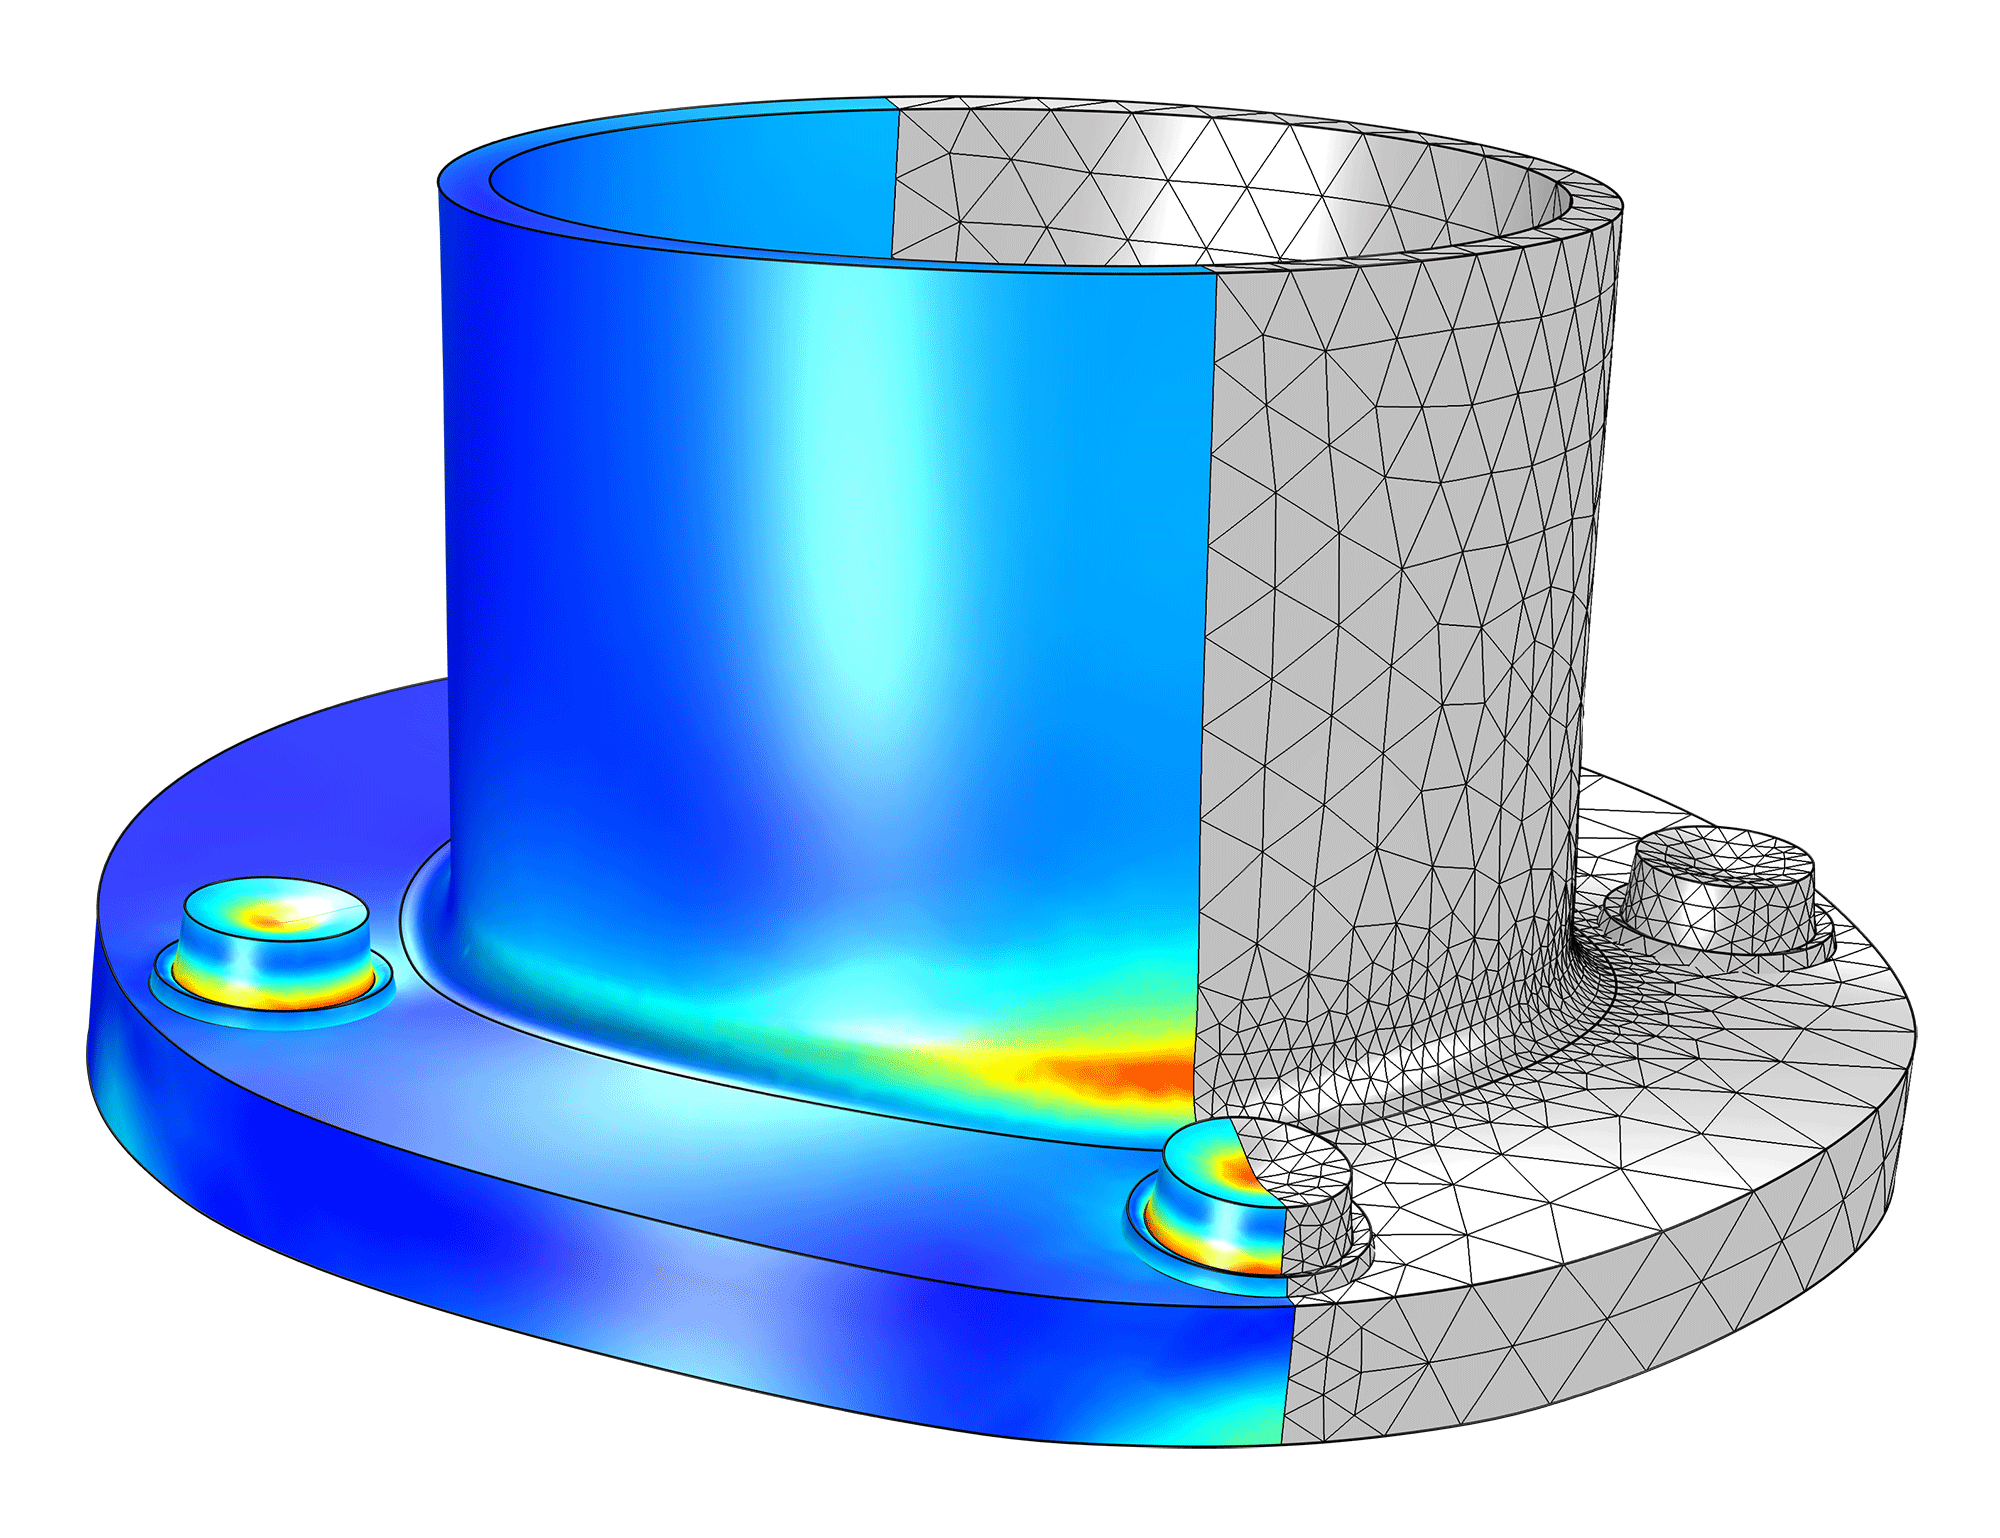
\includegraphics[scale=0.23]{pictures/tube-connection}
  \vfill
  \noindent
  \raggedleft{\Huge {ME 310: Mechanical Design I}}
  \vskip\baselineskip
  \noindent
  {\Large {Sappinandana Akamphon}}
\end{titlepage}
\restoregeometry % restores the geometry
\nopagecolor% Use this to restore the color pages to white

\chapter*{Preface}

The materials accumulated herein is intended for use as a reading and teaching references for ME 310: Mechanical Design I. The main objective of the class is to introduce students to the concepts of mechanical design by applying knowledge obtained in ME 210: Mechanics of Materials, coupled with the concept of basic load-bearing component design in this class.

In this textbook, students will be introduced to engineering design process and fundamental decisions that are involvd.  Basic review of engineering materials and its application in mechanical design is the next topic, with additional focus on material selection.

After the previous two chapter to introduce the design process, we brush up on important materials covered in Mechanics of Materials: axially loaded members, torsion, bending, and multiaxial stress analysis. This links to the next chapter, theories of failure, which completes all the theoretical knowledge required to tackle component design.

Component design is divided into load-bearing components (beams, shafts, columns, and mechanical springs) and joints (bolted and welded). Finally we step back and look at a bigger picture of component interaction and how design of one component can affect the design of another.

Lastly, the text cover a longstanding and ever-growing trend of computer-aided design by discussing the its basics and employing Solidworks as a reference software for basic finite element analysis and design tool.

\vspace{2cm}\hspace{10cm} Sappinandana Akamphon


\chapter*{Revisions}

\paragraph{July 2014}
Initial complete contents of Chapters 1 - 7.

\paragraph{March 2015}
Added Chapter 8.

\paragraph{August 2015}
Added Chapter 9.

\paragraph{April 2016}
Added Exercises in Chapters 1 - 2.

\paragraph{September 2016}
Added Chapters 10 and 11. Added exercises in Chapters 6 - 11.

\paragraph{February 2017}
Migrated to \LaTeX\ from Microsoft Word. Added original graphics for Chapters 3 - 10.

\paragraph{March 2018}
Converted examples to Python\TeX\ to prevent any miscalculations. Add appendices on sectional properties of structural steels and moments of inertia.

\tableofcontents

\listoffigures

\listoftables

\mainmatter

\part{The Preparations}

%%%%%%%%%%%%%%%%%%%%%%%%%%%%%%%%%%%%%%%%%%%%%%%%%%%%%%%%%%%%%%%%%%%%%%%%%%%%%%%%%%%%%%%%%%%%%%%%%%%%%%%%%%%%%%%%%%%%%%%%%%%%%%%%%%%%%%%%%%%%%%%%%%%%%%%%%%%%%%%%%%%%%%%%%%%%%%%%%%%%%%%%%%%%%%%%%%%%%%%

\chapter{Introduction to Engineering Design}

Engineering design is a process of applying science and engineering methods to define a structure or system in detail so that it can be made. The main objective of our contribution as mechanical engineers—mechanical design—includes determination of proper materials, dimensions, and shapes of the components so that they will support given loads and function properly.

A good design meets performance, cost, and safety requirements. An optimum design is the best solution to a design problem within given constraints. The objective function to optimize may be minimum weight, minimum volume, minimum cost, or other appropriate criteria. A typical design procedure involves

\begin{enumerate}
  \item Evaluate the mode of possible failure of components.
  \item Determine the relationship between the applied load and the resulting effect such as stress and deformation.
  \item Determine the maximum usable value of a significant quantity such as stress or deformation that may cause failure. Using this value together with equation(s) obtained from part 2 to determine allowable loads.
    \item Select the safety factor.
\end{enumerate}
        
The preceding procedure must be adjusted to each individual case, as certain steps may be unnecessary or obvious. No two design problems are exactly the same, and no two design solutions should be the same.

\section{Engineering Design Processes}

Solutions to design problems start at the very first with the recognition of problems or needs for a part, machine, or system. The problems or needs are then formulated into sets of requirements and constraints. In design problems, there are usually more than one right answer. Design considerations often require a trial-and-error process, as illustrated by \cref{fig: engineering design processes}.

\begin{figure}[h]
  \centering
  \smartdiagram[circular diagram:clockwise]{Ask, Research, Imagine, Plan, Create, Test, Improve}
  % 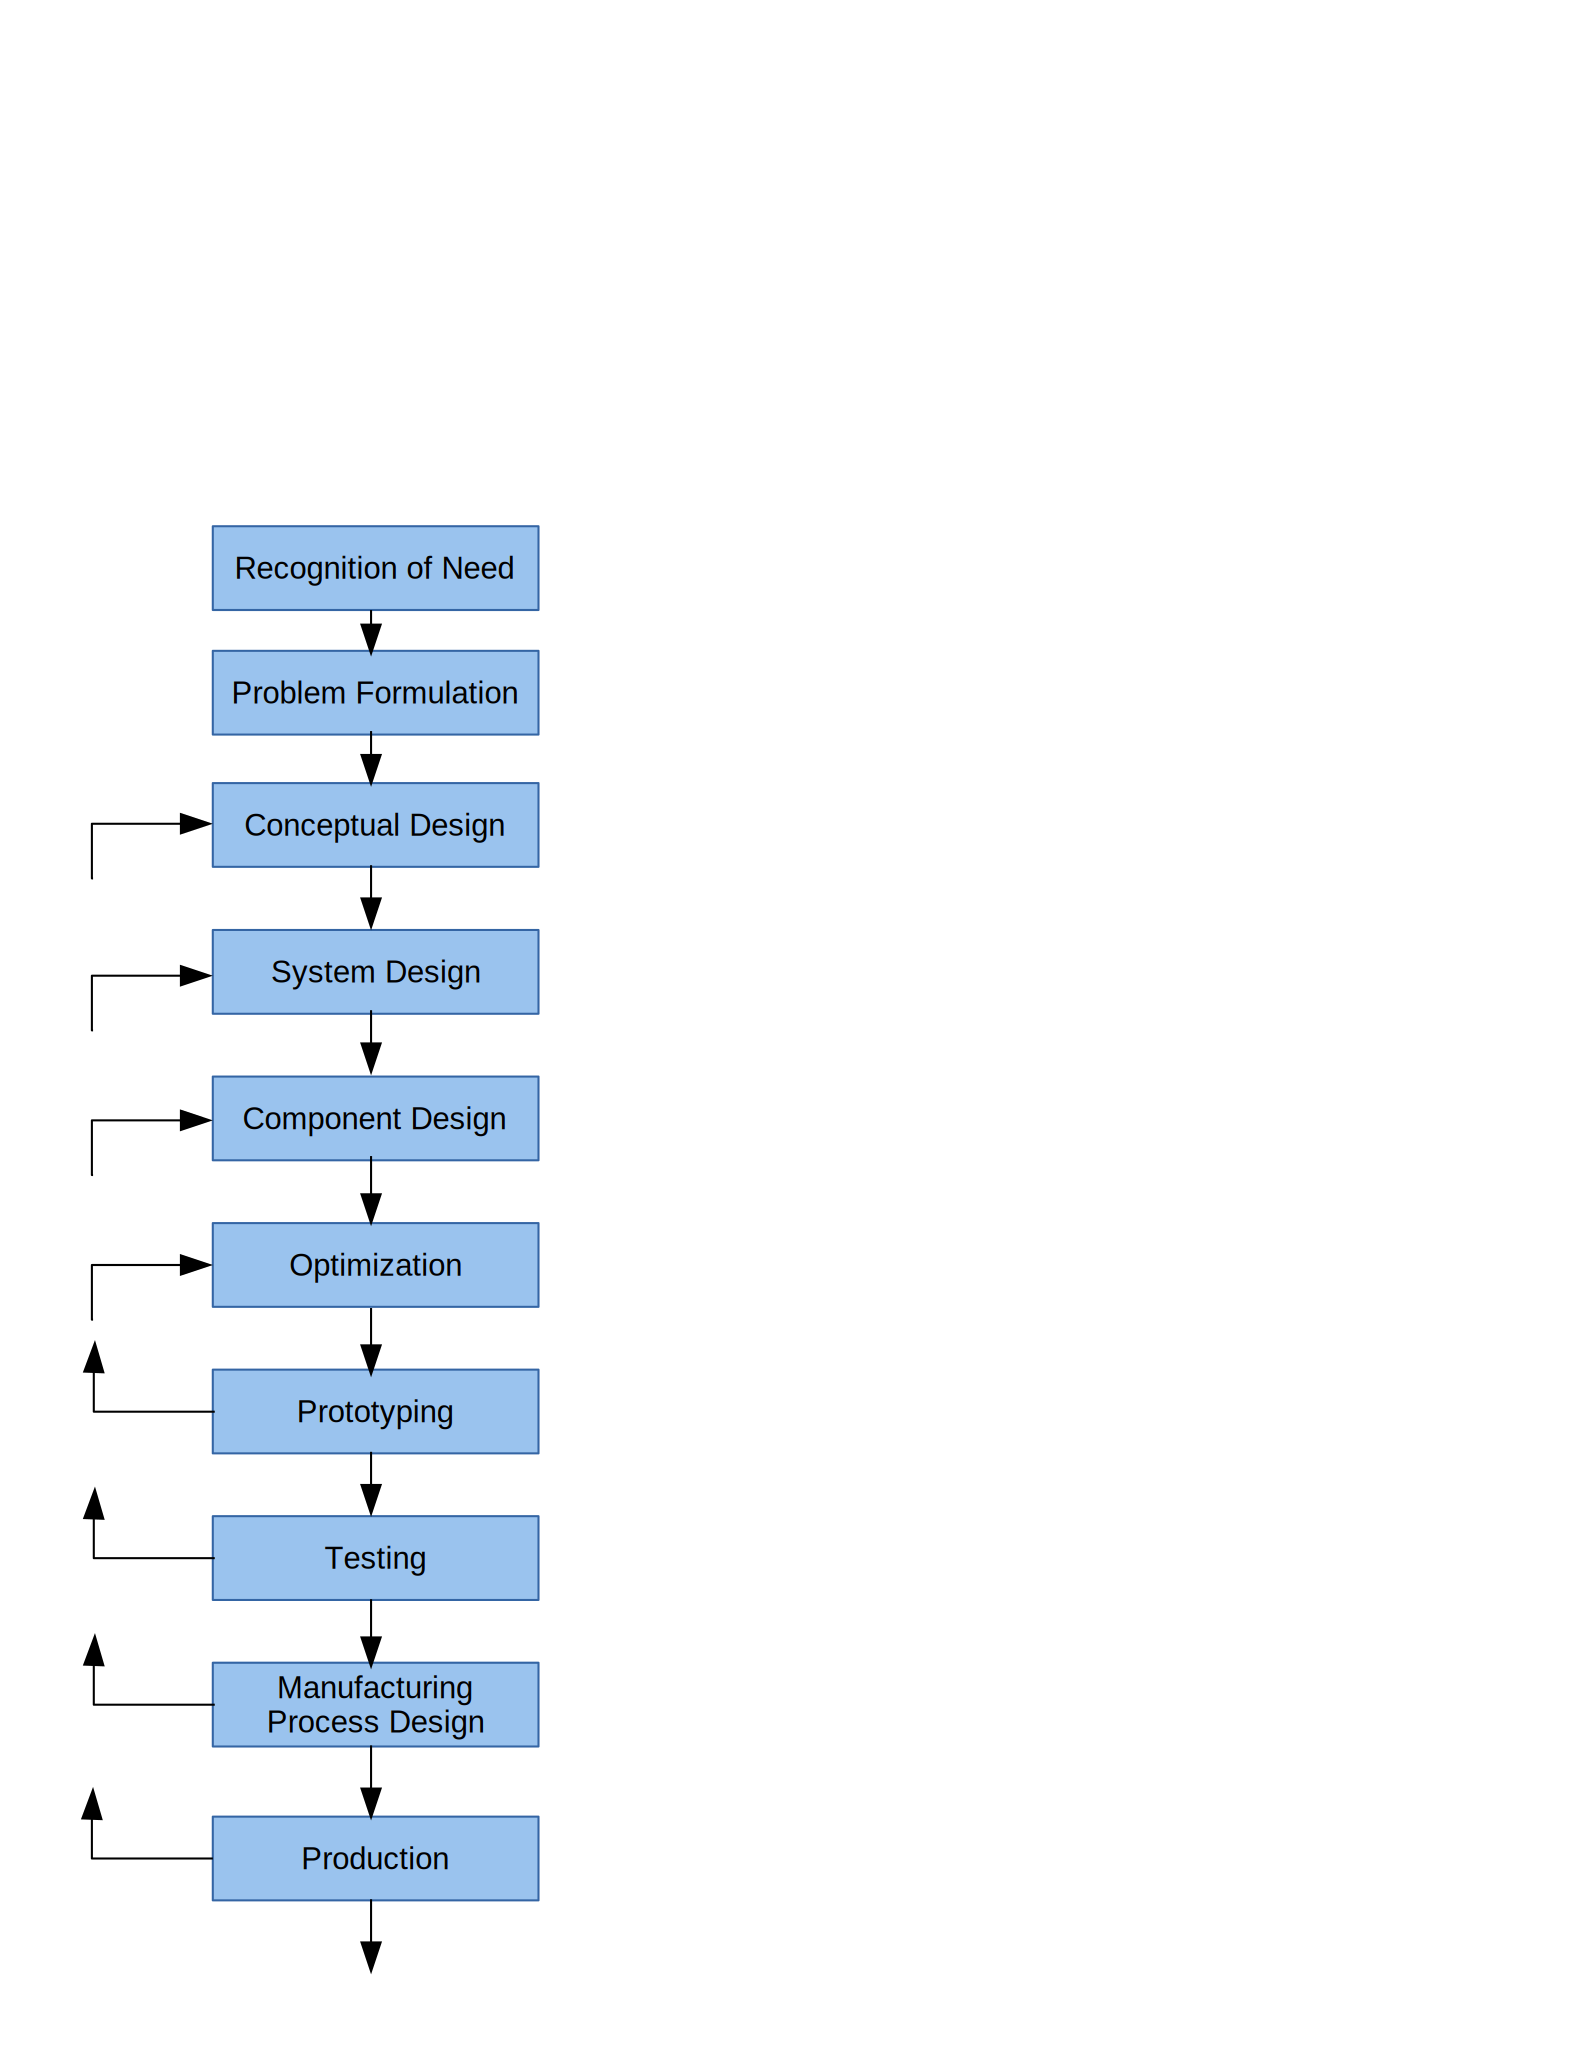
\includegraphics[scale=0.75]{pictures/intro-eng-design/eng-design-process}
  \caption{Flowchart of typical engineering design processes}
  \label{fig: engineering design processes}
\end{figure}

Product realization and production involve multiple, recursive, and sometimes, concurrent processes. There are also many possible backward loops where corrections need to be made in earlier stages of design. For example, during the prototyping period, it is found that two parts that are intended to mate do not fit together because they shrink during cooling. It may not be at all possible to change the manufacturing processes, in which case the components have to be redesigned to factor in the thermal shrinkage.

In this class, our efforts will be mainly focused on problem formulation, conceptual, system, and component design. Design optimization will also be discussed, though only in limited details.

To help facilitate the processes of problem formulation and conceptual design, a systematic method of determining and addressing requirements (both functional and mechanical) is needed. Constructing a FRDPARRC chart is one such method.

FRDPARRC (pronounced FRED-PARK) are initials of columns on a design chart to help designers tabulate various design considerations. The initials stand for FR (Functional Requirements), DP (Design Parameters), A (Analyses), R (References), R (Risks), and C (Countermeasures).

\begin{enumerate}
\item Functional Requirements: a list of independent functions that the design is to accomplish.
\item Design Parameters: ideally independent means to accomplish each functional requirement. A functional requirement can have multiple potential design parameters. The best one must eventually be selected.
\item Analyses: each potential design parameter’s feasibility must be proven by physical equations, finite element analysis, or experiments.
\item References: books, contacts, patents, or websites that can be used to verify and help develop the analyses.
\item Risks: possible complications and issues for each design parameters, ranked from high to low with explanations.
\item Countermeasures. ideas or plans to mitigate each risk whether original or off-the-shelf solutions.
\end{enumerate}

To use the chart, create one sheet to each functional requirement/design parameter pair. Map out all of the required analyses, references, risks, and countermeasures. Compare all of the potential design parameters and decide on the optimal one.

\begin{example}
  FRDPARRC sheet for a coconut meat extraction machine

  Design considerations for a coconut meat extraction machine for
  coconut milk production.
\end{example}

\begin{solution}
  Given that the final goal is to make coconut milk, which definitely will involve squeezing ground coconut meat, we will assume that leaving the meat on the shell does not affect the taste or quantity of coconut milk obtained. This opens up at least two possibilities to obtain ground coconut meat. The first is to scrape it off the shell, and the second is to grind the meat together with the shell. There may be other possible methods, but in this example we will only consider these two.
  \begin{center}
    \begin{tabular}{ L{4.5cm} L{4.5cm} L{4.5cm} }
      \toprule
      Functional Requirement & \multicolumn{2}{c}{Get coconut meat from hard shell and mince it} \\
      \midrule
      Design Parameters &  Scraping coconut meat &  Grinding coconut meat \\
      \midrule
      Analysis & Strength of meat \vfill Beam bending & Strength of shell \vfill Grinding teeth strength \\
      \midrule
      References &  Mechanics of Material &  Mechanics of Material \\
      \midrule
      Risks & Broken scraper &  Broken grinder teeth \vfill Stuck grinder blade \\
      \midrule
      Countermeasures & Strong material \vfill Safety factor  & Safety factor \vfill Allow proper clearance \\
      \bottomrule
    \end{tabular}
  \end{center}
\end{solution}

\begin{example} Design of a Lawn Mower

  Ahh.. Grass lawn maintenance. Very possibly one of the most budget consuming activities in Thailand household landscaping business considering how our greenspace tends to be mainly filled by small bushes and shrubs and square miles upon square miles of grass lawns. Keeping these laws nice and trimmed will be very time consuming without proper equipment. In the olden days, we may have two main options: a pair of grass shears (scissors) or a lawn mower.

  \begin{figure}[H]
    \centering
    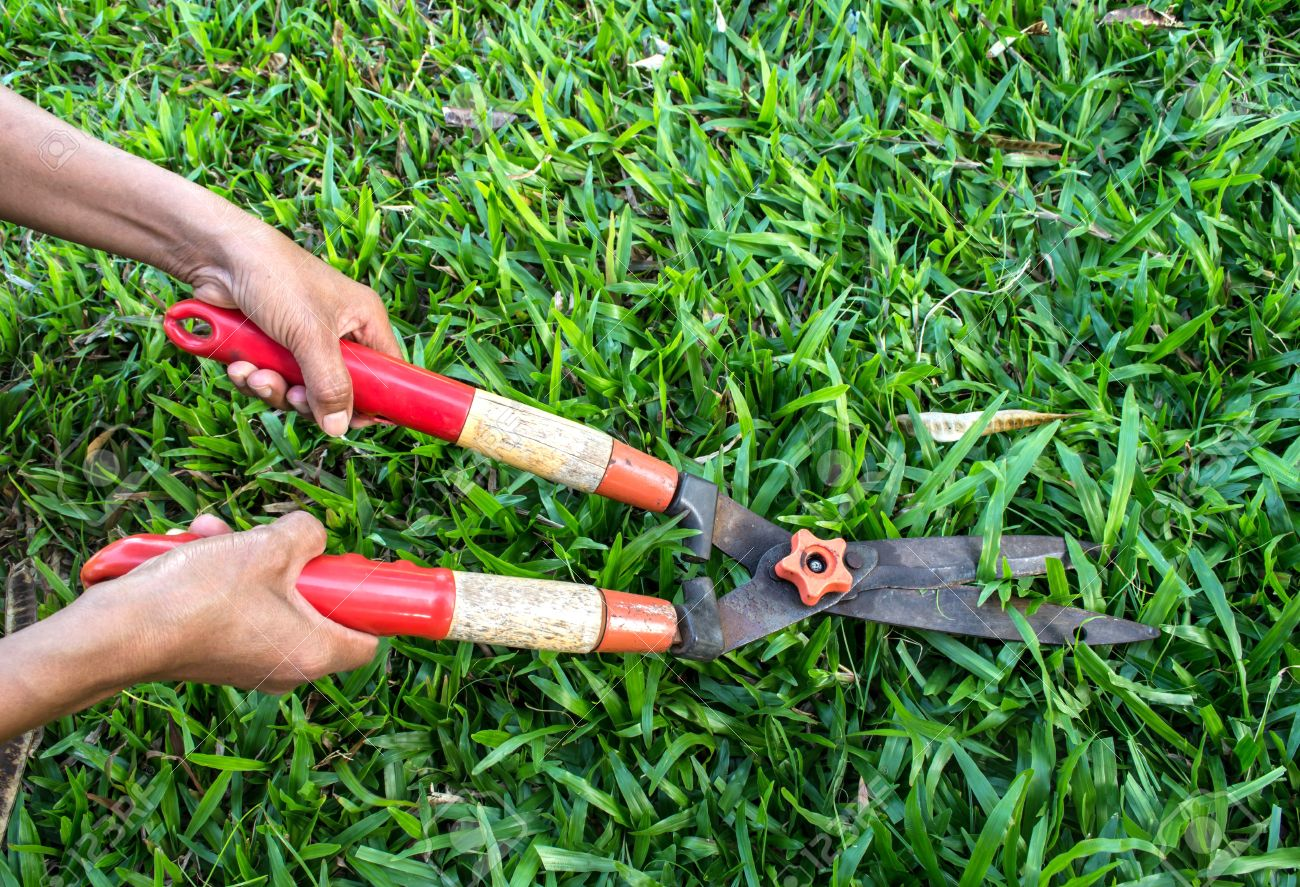
\includegraphics[width=0.4\textwidth]{pictures/intro-eng-design/grass-shears}
    \hspace{1cm}
    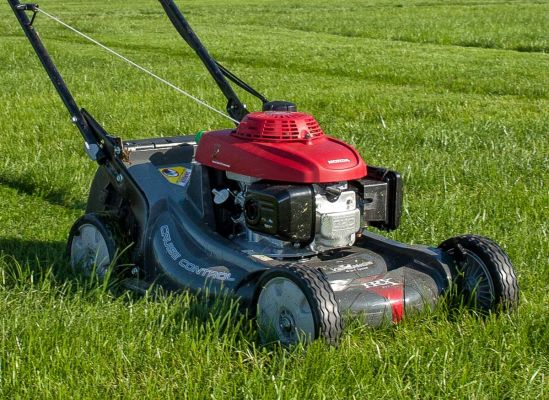
\includegraphics[width=0.4\textwidth]{pictures/intro-eng-design/lawn-mower}
  \end{figure}
  
  Now, each does have its own strength and weaknesses. Shears are very portable, but very slow. Mower, on the other hand, is very fast, but also very heavy. By \emph{recognizing} this gap between the two available solutions, we can start to \emph{formulate} the requirements to fill that void.
  
  \begin{figure}[H]
    \centering
    \begin{tikzpicture}
     \draw[->] (0,0) --++ (90:5) node[above left]{Speed};
     \draw[->] (0,0) --++ (0:5) node[above right]{Portability};
     \node at (1,3.5) [draw, circle, fill=LightGreen, minimum width=1.5cm, text width=1.5cm, align=center]{Lawn Mower};
     \node at (3.5,1) [draw, circle, fill=LightGreen, minimum width=1.5cm, text width=1.5cm, align=center]{Grass Shear};
     \node at (2.25,2.25) [draw, circle, fill=LightGreen, minimum width=1.5cm, text width=1.5cm, align=center]{??};
    \end{tikzpicture}
  \end{figure}

  Note that, obviously, there may be other factors that a customer considers in his grass cutting endeavor. For the purpose of this example, however, we will only consider speed and portability.

  The main component of a grass cutting tool is the cutting component. Both the shears and the mower use steel blades. The mower blade spins at high velocity, while grass shears rely on shearing (duh!). To increase portability, we must reduce the weight and load generated by the spinning steel blades.

  Grass is not terribly hard, we don't need thick steel to generate enough shear force to cut it. A spinning tough plastic wire will do that for a much smaller centrifugal load and weight.

  The final product is this.

  \begin{figure}[H]
    \centering
    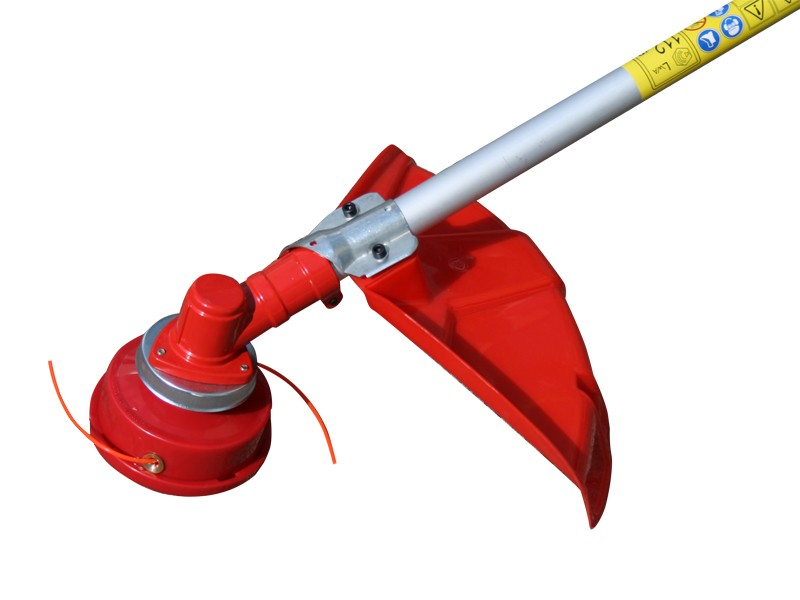
\includegraphics[width=0.5\textwidth]{pictures/intro-eng-design/cutter-wire}
  \end{figure}

  There are plenty of additional benefits to switching to wire cutting. Wires don't send rocks, pebbles, or dirt flying. Lighter cutting mechanism also means smaller motor and smaller energy source, further reducing the weight of the system.
\end{example}

\section{Safety Factor}

Occasionally, it is difficult to determine the numerous factors involved in various aspects of analysis and design of structures. A significant area of uncertainty is connected to the assumptions made in stress and deformation analyses. An equally important item is the nature of material failure. Added to the uncertainty of any problems are exogenous factors like types of loads, environmental effects, variations in material properties, consequences of failure, human safety and economics, and other considerations.

\subsection{Definition of Safety Factor}

Engineers use a safety factor to ensure against uncertainties involving strength and loading. This factor is employed to provide guarantee that the load applied to a component does not exceed the largest load it can support. The safety factor $N_s$ is therefore the ratio of the maximum load that produces failure of the member to the load allowed under service conditions.

\begin{equation}
  N_s = \frac{\text{failure load}}{\text{allowable load}}
\end{equation}

The allowable load is also called the service load or working load. This is the basic definition of the safety factor. This ratio must always be greater than 1 so that a designed component can just sustain the maximum load at failure.
A common approach to design is to use a safety factor with respect to the strength of the member. In most cases, the applied load and the stress produced with in the member are linearly related, if that is the case, the safety factor may also be defined by

\begin{equation}
  N_s = \frac{\text{material strength}}{\text{applied stress}}
\end{equation}

Here, the material strength is either a static or a dynamic property. When loading is static, the material strength represents either the yield strength of the ultimate strength, which will be discussed in Section 4.1. For repeated or dynamic loading, the material strength may be based on the endurance limit, discussed in Section 4.2. These definitions of safety factor are applicable for any type of member and loading condition. In some cases, more than one value of safety factor can exist because there may be more than one potential mode of failure for a member—one safety factor for each mode of failure. The smallest value of safety factor for any component is of the greatest concern because it is the most likely mode of failure.

\subsection{Selection of Safety Factors}

Choosing an appropriate safety factor to be used for a variety of applications is one of the most important engineering tasks. The selection of an appropriate value of safety factor is based primarily on the following five factors.

\begin{enumerate}
\item Degree of uncertainty about loading. In some situations, load can be determined with virtual certainty. The loads acting on an engine valve spring are definitely established by the valve open and valve close positions. But what loads should be used for the design of automotive suspension components, whose loads can vary tremendously depending on the severity of use?
\item Degree of uncertainty about material strength. Ideally, the engineer would have extensive data pertaining to the strength of the material as fabricated into the actual parts, and tested at temperatures and in environments similar to those actually encountered. But this is hardly ever the case. More often, available material strength data pertain to samples smaller in size, which has only tested at normal room temperature and has not been assembled. Even the available data itself is not a single value but more of a scatter.
\item Uncertainties in relating applied loads to material strength via stress analysis. Various assumptions involved with stress analysis from stress concentration to validity of failure theories may give rise to errors in the calculations.
\item Consequences of failure—human safety and economics. If the consequences of failure are catastrophic, relatively large safety factors much be used. Furthermore, if the failure of some relatively inexpensive part could cause extensive shutdown of a major assembly line, economics dictates increasing the cost of the part as much as necessary to virtually eliminate the possibility of failure.
\item Cost of providing a large safety factor. This cost involves a monetary consideration and may also involve important consumption of resources. In some cases, a safety factor larger than needed may have a serious consequences. A dramatic example is an aircraft with excessive safety factors, making it too heavy to fly. Another example is that it is possible to design an automobile that is so safe and strong that even a ‘crazy’ driver trying to wreck the car would barely cause a scratch. But in doing so, the designer would penalize ‘good’ drivers by making them pay for much too strong components than they need. The prohibitive price certainly would motivate them to buy competitor’s cars.
\item A key point in safety factor selection is balance. All parts of a machine or system should have consistent safety factors. Components that might possibly cause human injury or entail major costs should have the greatest safety factors; components that are comparable in these respects should generally have about the same safety factor, and so on.
\end{enumerate}

\subsection{Recommended Values for Safety Factors}

Keep in mind that this is by no means an absolute rule to follow--more of a general guideline for safety factor selection. After all, different applications and different impact failures will require that the designer reconsider the proper safety factor for a component. These factors are based on yield strength.

\begin{table}[h]
  \centering
  \caption{A guideline for appropriate selection of safety factor value.}
  \label{table: safety factor guideline}
  {\renewcommand{\arraystretch}{1.5}
  \begin{tabular}{ L{7cm} C{5cm} }
    \toprule
    \rowcolor{LightSkyBlue!70} Conditions & $N_{s\text{, cond}}$ \\
    \midrule
    Exceptionally reliable materials, controllable conditions, controlled loading (low weight a priority) & 1.25 – 1.5 \\
    \rowcolor{LightSkyBlue!50} Well-known materials, reasonably constant conditions, reliable loading & 1.5 – 2 \\
    Average materials, ordinary environments, determinable loading & 2 – 2.5 \\
    \rowcolor{LightSkyBlue!50} Lesser-known or brittle materials, average environment, determinable loading & 2.5 – 3 \\
    Untried materials under average conditions or known materials under uncertain environments and loading & 3 - 4 \\
    \rowcolor{LightSkyBlue!50} Repeated loading & Switch from yield to endurance limit \\
    Impact forces & Include impact factor \\
    \rowcolor{LightSkyBlue!50} Brittle materials (safety factor based on ultimate strength) & Double the safety factor \\
    \bottomrule
  \end{tabular}}
\end{table}

Note that this table mainly focuses on only the `cause' side of a mechanical failure--protecting against uncertainty from loading conditions, quality of design, and craftsmanship. However, as mentioned in 4) in selection criteria for safety factors, the cost of failure both to human safety and economics (the `result' side of a failure) should receive as much attention. ... presents the following guideline to consider additional safety factors based on the cost of mechanical falure.

\begin{table}[h]
  \centering
  \begin{tabular}{llccc}
    \toprule
    \multicolumn{2}{l}{\multirow{2}{2cm}{Characteristics}} & \multicolumn{3}{c}{Danger to Personnel} \\
    \cmidrule{3-5}
                                       &          & mild & moderate & severe \\
    \midrule
    \multirow{3}{3cm}{Economic Impact} & mild     & 1.0  & 1.2      & 1.4    \\
                                       & moderate & 1.0  & 1.3      & 1.5    \\
                                       & severe   & 1.2  & 1.4      & 1.6    \\
    \bottomrule
  \end{tabular}
  \caption{Safety factor consideration for human safety and economic impact}
  \label{tab: safety factor safety econ}
\end{table}

The total safety factor when considering both the design and operating conditions ($N_{s\text{, cond}}$) and the cost to human safety and economy ($N_{s\text{, cost}}$) is simply the product of the two individual factors.

\begin{equation}
  \label{eq: total safety factor}
  N_s = N_{s\text{, cond}} N_{s\text{, cost}}
\end{equation}

\begin{example}{Safety factor for a training bicycle for toddlers}

  We want to approximate a proper safety factor for a bicycle for toddlers (small children). Let us take a balance bike as shown in the figure below as an example.

  \begin{figure}[H]
    \centering
    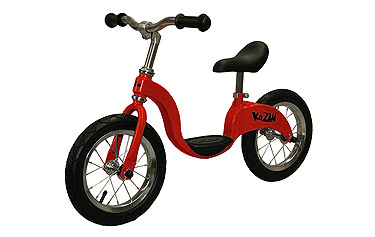
\includegraphics[width=0.5\textwidth]{pictures/intro-eng-design/balance-bike}
  \end{figure}
\end{example}
\begin{solution}

  While individual safety factors may require knowledge of materials and requirements for each component, we can discuss the safety factor of the \emph{system}. Referring to \cref{table: safety factor guideline}, this bicycle probably will be using common materials whose properties are well known and understood. However, being a children's toy, it can be subjected to some unexpected `operating conditions'. (You know, kids being kids, they will invent some ridiculous ways to play with their toys.) If we already expect this unexpected operating conditions, we can simply increase the loading requirement and file this under `reasonably constant conditions.' Combining the two, the safety factor from the design and operating conditions should fall between 1.5 - 2.

  Now, considerting safety and economic impact. This is a bike for toddler so accidents are likely to happen. Also toddlers are still small and weak so failure could have disastrous repercussions (severe). The cost of fixing the failure should be relatively low (mild), however, so the combined safety factor for human safety and economic impact is 1.4.
\end{solution}

\section*{Summary}

Engineering design is a process that combines technical knowledge with creativity. It is almost in equal parts science and imagination. Unlike many mathematical equations, design problems usually have multiple possible answers being equally right.

To design an object, one must first start off by observing and realizing the need for such objects. Several concepts are then developed and the best candidate is picked using basic analysis. Once that has been done, each components should be thoroughly analyzed and optimized for the design purpose. This part must be done while considering many factors such as required strength, ergonomics, and material availability. The designer must all so consider the manufacturing processes and assembly involved, gauging their feasibility. Prototyping and testing follow, though there are at times corrections and modifications that must be addressed.

Designing is multidisciplinary, requiring various branches of engineering. A good design must properly deal with uncertainty and variability from the designer, supplier, manufacturer, and end user sides. To do so, proper calculation techniques and safety factors must be incorporated. A good design satisfies all required, nonnegotiable constraints while optimizes negotiable ones.

\section*{Exercises}

\begin{exercises}
  
  \exercise Consider the problem of portable personal transportation (transportation options for one passenger). Determine some of the basic required functions. Draw a FRDPARRC sheet of the problem and fill them out for with at least 2 conceptual designs.

  \exercise What would be proper safety factors of the following components?
  \begin{enumerate}
  \item An elevator cable
  \item Mobile phone case
  \item Umbrella shaft
  \item Passenger car front bumper
  \item Airplane fuselage
  \end{enumerate}
  Elaborate on your reasoning. Think about the materials will you choose for the components and their operating conditions. Factor those into your ‘proper’ safety factor.

\end{exercises}

%%%%%%%%%%%%%%%%%%%%%%%%%%%%%%%%%%%%%%%%%%%%%%%%%%%%%%%%%%%%%%%%%%%%%%%%%%%%%%%%%%%%%%%%%%%%%%%%%%%%%%%%%%%%%%%%%%%%%%%%%%%%%%%%%%%%%%%%%%%%%%%%%%%%%%%%%%%%%%%%%%%%%%%%%%%%%%%%%%%%%%%%%%%%%%%%%%%%%%%%%%%%%%%%%%%%%%%%%%%%%%%%%
 
\chapter{Material Selection}

The selection of materials and the processes used in manufacturing are important in the design of any machine component. Strength and stiffness are typically two key factors considered in the selection of a material. In recent years, choices of materials have been increasingly influenced by recyclability, energy requirements, and environmental pollution. Additionally, cost and availability are also important. When considering cost, simply considering the material cost is sufficient. Material choices tend to dictate manufacturing processes involved, which in turn influence the total cost of a fabricated part. With new materials emerging constantly, designers are often required to consider the tradeoffs between overall performance and total cost.

This chapter attempts to summarize some of the basic information and to emphasize the increasing importance of a rational approach to the use of empirical material properties data. A material property database is available at \url{http://www.matweb.com}. The database includes information on steel, aluminum, titanium, and zinc alloys, superalloys, ceramics, thermoplastics, and thermoset polymers. Another site \url{http://www.machinedesign.com} presents general information on plastics, composites, elastomers, nonferrous metals, ferrous metals, and ceramics.

\section{Cast Iron}

Cast iron is a four-element alloy containing iron, carbon, silicon, and manganese. Additional alloying elements are sometimes added. The physical properties of a cast iron are strongly influenced by its cooling rate during solidification. This depends on the size and shape of the casting and on details of foundry practice. Because of this, cast iron is usually specified by its mechanical properties rather than by chemical analysis.

The distinctive properties of cast iron result from its carbon content. High carbon content makes molten iron very fluid and easy to be poured into complex shapes. The precipitation of carbon during solidification reduces shrinkage normally found in other materials. The presence of graphite in the metal provides excellent machinability even at extreme hardness level, reduces vibration, and lubricates wearing surfaces. When the heat is removed rapidly, most of the carbon at the surface remains combined as iron carbides, which are extremely hard and wear-resistant.

\subsection{Grey Iron}

The appearance of gray iron comes from precipitated carbon in the form of graphite. Gray iron has good wear resistance. Even stronger resistance can be obtained through various foundry techniques, heat treatment, or additional alloying elements. While graphite can significantly weaken cast iron in tension, it can improve the compressive strength markedly. This advantage is very useful in construction of members under bending.

Typical applications of gray iron include engine blocks, machine bases and frames, gears, flywheels, and brake disks and drums.

\subsection{Ductile (Nodular) Iron}

Ductile iron is alloyed with magnesium, which causes excess carbon to precipitate in the form of small spheres or nodules. These nodules do not disrupt the structure as much as graphite flakes in gray iron do, thus giving good ductility along with improved tensile strength, stiffness, and impact resistance. Ductile iron is specified by three numbers, as 60 – 40 – 18, which denote tensile strength (60 ksi), yield strength (40 ksi), and elongation (18 percent).

Typical applications include engine crankshafts, heavy-duty gears, and hardware items such as automobile door hinges.

\subsection{White Iron}

White iron (based on their white appearances of fracture surfaces) is produced in outer portion of gray and ductile iron castings by chilling selected surfaces of the mold, thereby denying time for carbon precipitation. The resulting structure is extremely hard, wear-resistant, and brittle.

Typical applications are found in ball mills, extrusion dies, cement mixer liners, railroad brake shoes, rolling mill rolls, crushers, and pulverizers.

\subsection{Malleable Iron}

Typical uses are for heavy-duty parts having bearing surfaces, which are needed in trucks, railroad equipment, construction machinery, and farm equipment.

Mechanical properties and qualities of selected cast irons are tabulated in \cref{tab: cast iron quals} and \cref{tab: cast iron props}, respectively.

\begin{table}[H]
  \centering
  \begin{tabular}{lll}
    \toprule
    \multirow{2}{2cm}{Name} & Nominal composition & \multirow{2}{3.5cm}{Form and condition} \\
                            & {[}\% by weight{]} & \\
    \midrule
    Grey cast iron (ASTM A48) & C 3.4, Si 1.8, Mn 0.5                  & Cast \\
    White cast iron           & C 3.4, Si 0.7, Mn 0.6                  & Cast (as cast) \\
    Malleable iron (ASTM A47) & C 2.5, Si 1.0, Mn 0.55                 & Cast (annealed) \\
    Nodular iron              & C 3.4, P 0.1, Mn 0.4, Ni 1.0, Mg 0.06  & Cast \\
    Nodular iron (ASTM A339)  & —                                      & cast (quench tempered) \\
    Ni-hard type 2            & C 2.7, Si 0.6, Mn 0.5, Ni 4.5, Cr 2.0  & Sand-cast \\
    Ni-resist type 2          & C 3.0, Si 2.0, Mn 1.0, Ni 20.0, Cr 2.5 & Cast \\
    \bottomrule
  \end{tabular}
  \caption{Comparative qualities of cast irons \cite*{plisga2017standard}}
  \label{tab: cast iron quals}
\end{table}

\begin{table}[H]
  \centering
  \begin{tabular}{lcccc}
    \toprule
    \multirow{2}{2cm}{Name} & Yield strength & Tensile strength & Elongation & Hardness \\
                            & {[}ksi{]} & {[}ksi{]} & {[}\% (in 2 inches){]} & {[}Brinell scale{]} \\
    \midrule
    Grey cast iron (ASTM A48) & — & 50 & 0.5 & 260 \\
    White cast iron & — & 25 & 0 & 450 \\
    Malleable iron (ASTM A47) & 33 & 52 & 12 & 130 \\
    Nodular iron & 53 & 70 & 18 & 170 \\
    Nodular iron (ASTM A339) & 108 & 135 & 5 & 310 \\
    Ni-hard type 2 & — & 55 & — & 550 \\
    Ni-resist type 2 & — & 27 & 2 & 140 \\
    \bottomrule
  \end{tabular}
  \caption{Comparative mechanical properties of cast irons \cite{plisga2017standard}}
  \label{tab: cast iron props}
\end{table}

\section{Steel}

Steel is the most extensively used material for machine components. By varying the composition, thermal treatment, and mechanical treatment, manufacturers can obtain a wide range of mechanical properties. Three basic relationships are fundamental to the appropriate selection of steel composition.

\begin{enumerate}
\item All steels have essentially the same Young’s moduli. Therefore, if the main concern is the stiffness or rigidity of the component, all steels should perform equally well and the least costly in terms of both material and fabrication costs should be selected.
\item Carbon content mainly determines the hardness of steel. Maximum hardness increases with carbon content up to about 0.7\%, so small and regularly shaped parts can be heat-treated to give almost identical hardness and strength with plain carbon steel as with more expensive alloy steels.
\item Alloying elements (manganese, molybdenum, chromium, nickel, and others) improve the ease with which steel can be hardened. With these alloys, the potential hardness and strength can be realized with less extreme heat treatments. This means that parts with large sections can achieve higher hardnesses in the core of the section and that irregularly shaped parts can achieve desired hardness from a more moderate heat treatment with lower risk from warpage from extreme temperatures.
\end{enumerate}

Through efforts to standardize a numbering system by the American Iron and Steel Institute (AISI) and the Society of Automotive Engineers (SAE), the AISI/SAE steel grades were established and since 1995 the future maintenance of the system was turned over to SAE. According to the grades, Carbon steels and alloy steels are designated a four digit number, whereby the first digit indicates the main alloying elements, the second digit indicates top grade elements, and the last two digits indicate the amount of carbon in hundredths of a percent by weight. An ``H'' suffix can be added to any designation to denote hardenability is a major requirement.

\begin{table}[h]
  \centering
  \begin{tabular}{rl}
    \toprule
    SAE designation & \multicolumn{1}{c}{Type} \\
    \midrule
    1xxx & Carbon steels \\
    2xxx & Nickel steels \\
    3xxx & Nickel-chromium steels \\
    4xxx & Molybdenum steels \\
    5xxx & Chromium steels \\
    6xxx & Chromium-vanadium steels \\
    7xxx & Tungsten steels \\
    8xxx & Nickel-chromium-molybdenum steels \\
    9xxx & Silicon-manganese steels \\ 
    \bottomrule
  \end{tabular}
  \caption{Major classifications of steel \cite{jeffus2011welding}}
  \label{tab: major class of steel}
\end{table}

\subsection{Plain Carbon Steels}

Plain carbon steels contain only carbon as a significant alloying element. Low-carbon steels have less than 0.3 percent carbon, medium-carbon steels have 0.3 – 0.5 percent, and high-carbon steels have above 0.5 percent.

\begin{table}[h]
  \centering
  \begin{tabular}{clp{8cm}}
    \toprule
    \% carbon & Classification & Typical Uses \\
    \midrule
    0.05 & Dead mild steel & Sheet and strip for presswork, car bodies, tin plate; wire, rod, and tubes \\
    0.08 - 0.15 & Mild steel & Sheet and strip for presswork; wire and rod for nails, screws, concrete reinforcement bar \\
    0.15 & Mild steel & Case carburising quality \\
    0.1 - 0.3 & Mild steel & Steel plate and sections, for structural work \\
    0.25 - 0.4 & Medium carbon steel & Bright drawn bar \\
    0.3 - 0.45 & Medium carbon steel & Shafts and high-tensile tubing \\
    0.4 - 0.5 & Medium carbon steel & Shafts, gears, railway tyres \\
    0.55 - 0.65 & High carbon steel & Forging dies, railway rails, springs \\
    0.65 - 0.75 & High carbon steel & Hammers, saws, cylinder linings \\
    0.75 - 0.85 & High carbon steel & Cold chisels, forging die blocks \\
    0.85 - 0.95 & High carbon steel & Punches, shear blades, high-tensile wire \\
    0.95 - 1.1 & High carbon steel & Knives, axes, picks, screwing dies and taps, milling cutters \\
    1.1 - 1.4 & High carbon steel & Ball bearings, drills, wood-cutting and metal-cutting tools, razors \\
    \bottomrule
  \end{tabular}
  \caption{Carbon steel classification and uses by carbon content}
  \label{tab: carbon steel classification}
\end{table}

\subsection{Alloy Steels}

Addition of alloying elements to steel is done to increase strength or hardenability, or achieving a special properties such as corrosion resisntance or extreme temperature stability.

In the case of increasing hardenability, \Cref{table: effective alloys} represents the results of a study by \citeauthor{datsko1977materials} of the relative effectiveness of various alloying elements in increasing hardenability to steel. The equations give a relative hardenability factor $f$ as a function of the concentration of the element used. 

\begin{table}[h]
  \centering
  \caption{Relative effectiveness of various alloying elements \cite{datsko1977materials}}
  \label{table: effective alloys}
  {\renewcommand{\arraystretch}{1.4}
    \begin{tabular}{lll}
      \toprule
      Alloying Element & Concentration & Relative Effectiveness \\
      \midrule
      Boron & $B < 0.002$ & $f_B = 17.23B^{0.0268}$\\
      Manganese & $Mn < 1.2$ & $f_{Mn} = 3.46Mn + 1$ \\
      Manganese & $1.2 < M\!n < 2.0$ & $f_{Mn} = 5.125M\!n - 1$ \\
      Molybdenum & $M\!o < 1.0$ & $f_{Mo} = 3.0M\!o + 1$ \\
      Chromium & $Cr < 2.0$ & $f_{Cr} = 2.18Cr + 1$ \\
      Silicon & $Si < 2.0$ & $f_{Si} = 0.7Si + 1$ \\
      Nickel & $Ni < 2.0$ & $f_{Ni} = 0.4Ni + 1$ \\
    \bottomrule
  \end{tabular}}
\end{table}

\subsection{HSLA Steels}

High-strength low-alloy (HSLA) steels were developed to provide better mechanical properties and/or greater corrosion resistance than carbon steels. They also differ from other steels in that they are not made to meet a specific chemical composition, but rather to a specific mechanical properties. They have carbon content between 0.05 - 0.25\% to retain formability and weldability. There can be other alloying elements including up to 2\% manganese and small quantities of copper, nickel, chromium, molybdenum, etc.

In many applications, their greater strength compared to plain carbon steel allows a considerable weight reduction with relatively small increase in total cost of the part. Their main use nowadays still remains in the automotive industry.

\subsection{Case-Hardening Steels}

Case hardening is a hardening of only the surface material (the case). It is usually accomplished by carburizing, cyaniding, nitriding, induction hardening, or flame hardening.

Carburizing is a process that introduces additional carbon into the surface of a low-carbon steel and then heat-treats it to obtain a high surface hardness.

Cyaniding is a similar process that adds nitrogen as well as carbon to the surfaces of low- and medium-carbon steels.

Nitriding adds nitrogen to an already machined and heat-treated part. The temperature of the process is 1000$^{\circ}$F (538$^{\circ}$C) or less, and no quenching is involved. This feature eliminates possible distortion problems. For maximum case hardness, special “nitralloy” steels (containing aluminum as an alloy) are often used. Medium-carbon alloy steels (notably 4340) are also nitrided. Induction hardening and flame hardening heat only the surfaces of parts made of medium-carbon and alloy steels, then quenching and tempering.

Induction hardening and flame hardening heat only the surfaces of parts made of medium-carbon and alloy steels, then quenching and tempering.

\subsection{Stainless Steels}

Stainless steels contain, by definition, a minimum of 10.5 percent chromium. Wrought stainless steels are austenitic, ferritic, martensitic, or precipitation hardening. Cast stainless steels are usually classed as heat-resistant or corrosion-resistant.

\subsection{Iron-Based Superalloys}

Iron-based superalloys are used primarily for elevated temperature applications, as in turbines. Some authorities consider only the austenitic materials to be true superalloys. In general, they are used at temperatures above 1000$^{\circ}$F (538$^{\circ}$C), and the martensitic materials are used at lower temperatures. Significant properties of superalloys include at high temperatures strength and resistance to creep, oxidation, corrosion, and wear. Typical uses are for parts (including bolts) of gas turbines, jet engines, heat exchangers, and furnaces.

\section{Nonferrous Alloys}

\subsection{Aluminum Alloys}

Literally hundreds of aluminum alloys are available, in both wrought and cast forms. The chemical composition of aluminum alloys is designated by four digits for wrought forms and by three digits for cast alloys. Thermal treatment, mechanical treatment, or both are indicated by a temper designation that follows the alloy identification number. The heat treatment of aluminum alloys to increase hardness and strength is quite different from the heat treatment of steel. Aluminum alloys are first held at an elevated temperature long enough to bring the hardening constituents (as Cu, Mg, Mn, Si, Ni) into solution, then quenched, and finally age-hardened. The latter causes some of the hardening elements to precipitate throughout the structure. Some alloys precipitate at room temperature; others require an elevated temperature (artificial aging). Although aluminum is a readily castable metal serving a host of useful applications, casting problems do exist. Shrinkage during casting is relatively large (3.5 to 8.5 percent by volume), and there is no mechanism analogous to the beneficial carbon precipitation in cast iron to counteract shrinkage. Hot shortness and gas absorption can be problems unless details of appropriate foundry practice are specified and controlled.

\subsection{Copper Alloys}

Copper alloys include a variety of brasses, alloys made principally of copper and zinc, and bronzes, alloys made principally of copper and tin. As a class, copper alloys have good electrical conductivity, thermal conductivity, and resistance to corrosion, but relatively low ratios of strength to weight. They can be hot- or cold-worked, but they strain-harden in the process. Ductility can be restored by annealing or by heat associated with welding or brazing. Specific desired properties, such as greater strength, resistance to heat softening, and machinability, can often be markedly improved by adding small amounts of additional alloying agents.

\subsection{Magnesium Alloys}

Magnesium alloys are the lightest engineering metals. They are designated by a system established by the American Society for Testing and Materials (ASTM), which covers both chemical composition and tempers. The designation begins with two letters representing alloying elements of the greatest and second greatest concentration. The letter designations are

\begin{table}[h]
  \centering
  \begin{tabular}{ C{3cm} C{3cm} C{3cm} }
    \hline
    A – Aluminum & K – Zirconium & Q – Silver \\
    E – Rare earths & L – Lithium & S – Silicon \\
    H – Thorium & M – Manganese & Z – Zinc \\
    \hline
  \end{tabular}
\end{table}

Next are two digits that represent the respective percentages of these two elements, rounded off to whole numbers. Following these digits is a serial letter that indicates some variation in composition or minor alloying constituents or impurities. For example, alloy AZ31B-H24 contains 3 percent aluminum, 1 percent zinc, and is strain-hardened.

\subsection{Nickel Alloys and Nickel-Based Superalloys}

Nickel alloys are used in a variety of structural applications that usually require specific corrosion resistance, and strength and toughness at temperature extremes as great as 2000$^{\circ}$F (1093$^{\circ}$C) and as low as -400$^{\circ}$F (-240$^{\circ}$C). Typical physical properties are given in Appendix C-15. The nickel and Duranickel alloys contain over 94 percent nickel. Monel represents a series of nickel–copper alloys, based on the mutual solubility of these two elements in all proportions. They are strong and tough at subzero temperatures, and especially resistant to stress corrosion cracking. Hastelloy designates a series of Ni–Mo and Ni–Mo–Cr superalloys. Several Hastelloys resist oxidation and maintain useful strength and creep properties in the range of 2000$^{\circ}$F (1093$^{\circ}$C). The Inconel, Incoloy, Rene, and Udimet alloys are Ni–Cr and Ni–Cr–Fe alloys. 

\subsection{Titanium Alloys}

Titanium alloys are nonmagnetic and extremely corrosion-resistant, have low thermal conductivity, and have outstanding strength-weight ratios. On the negative side, they are very expensive and difficult to machine. 

\subsection{Zinc Alloys}

Zinc is a relatively inexpensive metal with moderate strength. It has a low melting temperature and so is readily and economically die-cast. Typical zinc die castings include automotive parts, building hardware, office machine components, and toys. Limited use is made of the metal in other forms.

\section{Plastics}

Plastics constitute a large and varied group of synthetic organic materials. The basic chemical units of plastic materials are monomers. Under appropriate conditions, usually involving heat, pressure, or both, polymerization takes place, combining monomers into polymers. Typical monomers and their corresponding repeating polymer units are shown in \cref{fig: polymers and repeating units}.

\begin{figure}[h]
  \centering
  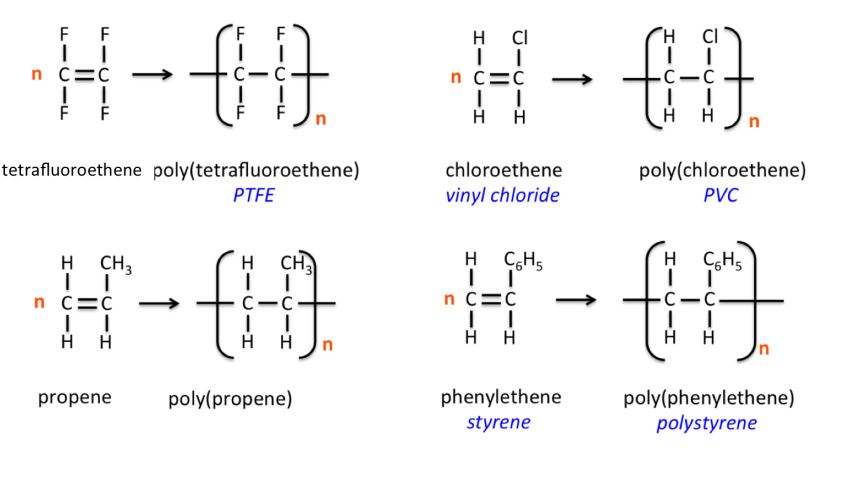
\includegraphics[scale=0.5]{pictures/Material-selection/polymer}
  \caption{Monomers and repeating polymer units of common polymers. \cite{secondaryscience4all}}
  \label{fig: polymers and repeating units}
\end{figure}
 
The addition of more and more monomers to form longer and longer polymer chains increases molecular weight and vastly alters physical properties. For example, Figure 3.10 shows $\text{CH}_4$, which is methane gas. Adding one $\text{CH}_2$ unit gives heavier ethane gas (C$_2$H$_6$). Continued addition of $\text{CH}_2$ units gives pentane, a liquid ($\text{C}_5\text{H}_{12}$), and paraffin wax ($\text{C}_{18}\text{H}_{38}$). At approximately $\text{C}_{100}\text{H}_{202}$, the material is tough enough to be a useful plastic, known as low-molecular-weight polyethylene. The toughest polyethylene, called high-molecular-weight polyethylene, contains nearly a half-million $\text{CH}_2$ units in a single polymer chain.

Polymer chain structures can incorporate side branching, also shown in Figure 2.2. The degree of branching influences the closeness with which the chains fit together. This, in turn, influences physical properties. Minimal branching promotes tight packing of the polymer chains (hence, strong intermolecular attractive forces), giving relatively high density, rigid crystalline structures, and also relatively extensive mold shrinkage. Extensive branching produces a more flexible, amorphous material with less mold shrinkage and distortion. Physical properties of the finished plastic can also be altered by copolymerization, the building of polymer chains with two monomers, and by alloying, a strictly mechanical mixing or blending of constituents which does not involve chemical bonds. 
 
Plastics have traditionally been designated as thermoplastic, softening with heat, and thermosetting, not softening with heat. A preferred designation is linear and cross-linked. The polymer chains in linear plastics remain linear and separate after molding. The chains in cross-linked plastics are initially linear but become joined irreversibly during molding into an interconnected molecular network.

Cross-linking can be initiated by heat, chemical agents, irradiation, or a combination of these. Some plastics can be either cross-linked or linear. The cross-linked form is more resistant to heat, chemical attack, and creep (better dimensional stability). On the other hand, the linear form is less brittle (more impact-resistant), more easily processed, and better adapted to complex shapes.

Recall that thermoplastics are generally impact resistant; thermosets are generally heat resistant.

\subsection{Thermoplastics}

\begin{itemize}[label=\scriptsize$\square$]

\item ABS (acrylonitrile–butadiene–styrene): Very tough, yet hard and rigid; fair chemical resistance; little water absorption, hence good dimensional stability; high abrasion resistance; easily electroplated.

\item Acetal: Very strong, stiff engineering plastic with exceptional dimensional stability and resistance to creep and vibration fatigue; low coefficient of friction; high resistance to abrasion and chemicals; retains most properties when immersed in hot water; little tendency to stress-crack.

\item Acrylic: High optical clarity; excellent resistance to outdoor weathering; hard, glossy surface; excellent electrical properties, fair chemical resistance; available in brilliant, transparent colors.

\item Cellulosics: Family of tough, hard materials; cellulose acetate, propionate, butyrate, and ethyl cellulose. Property ranges are broad because of compounding; available with various degrees of weather, moisture, and chemical resistance; fair to poor dimensional stability; brilliant colors.

\item Fluoroplastics: Large family (PTFE, FEP, PFA, CTFE, ECTFE, ETFE, and PVDF) of materials characterized by excellent electrical and chemical resistance, low friction, and outstanding stability at high temperatures; strength is low to moderate; cost is high.

\item Nylon (polyamide): Family of engineering resins having outstanding toughness and wear resistance; low coefficient of friction, and excellent electrical properties and chemical resistance. Resins are hygroscopic; dimensional stability is poorer than that of most other engineering plastics. 

\item Phenylene Oxide: Excellent dimensional stability (very little moisture absorption); superior mechanical and electrical properties over a wide temperature range. Resists most chemicals but is attacked by some hydrocarbons.

\item Polycarbonate: Highest impact resistance of any rigid, transparent plastic; excellent outdoor stability and resistance to creep under load; fair chemical resistance; some aromatic solvents cause stress cracking.

\item Polyester: Excellent dimensional stability, electrical properties, toughness, and chemical resistance, except to strong acids or bases; notch-sensitive; not suitable for outdoor use or for service in hot water; also available in thermosetting formulations.

\item Polyethylene: Wide variety of grades: low-, medium-, and high-density formulations. LD types are flexible and tough. MD and HD types are stronger, harder, and more rigid; all are lightweight, easy-to-process, low-cost materials; poor dimensional stability and heat resistance; excellent chemical resistance and electrical properties. Also available in ultrahigh-molecular-weight grades.

\item Polyimide: Outstanding resistance to heat (500 F continuous, 900 F intermittent) and to heat aging. High impact strength and wear resistance; low coefficient of thermal expansion; excellent electrical properties; difficult to process by conventional methods; high cost.

\item Polyphenylene Sulfide: Outstanding chemical and heat resistance (450 F continuous); excellent low-temperature strength; inert to most chemicals over a wide temperature range; inherently flame-retardant; requires high processing temperature.

\item Polypropylene: Outstanding resistance to flex and stress cracking; excellent chemical resistance and electrical properties; good impact strength above 15 F; good thermal stability; light weight, low cost, can be electroplated.

\item Polystyrene: Low-cost, easy-to-process, rigid, crystal-clear, brittle material; little moisture absorption, low heat resistance, poor outdoor stability; often modified to improve heat or impact resistance.

\item Polysulfone: Highest heat deflection temperature of melt-processible thermoplastics; requires high processing temperature; tough (but notch-sensitive), strong, and stiff; excellent electrical properties and dimensional stability, even at high temperature; can be electroplated; high cost.

\item Polyurethane: Tough, extremely abrasion-resistant and impact-resistant material; good electrical properties and chemical resistance; can be made into films, solid moldings, or flexible foams; ultraviolet exposure produces brittleness, lower properties, and yellowing; also made in thermoset formulations.

\item Polyvinyl Chloride (PVC): Many formulations available; rigid grades are hard, tough, and have excellent electrical properties, outdoor stability, and resistance to moisture and chemicals; flexible grades are easier to process but have lower properties; heat resistance is low to moderate for most types of PVC; low cost.

\end{itemize}

\subsection{Thermosets}

\begin{itemize}[label=\scriptsize$\square$]
\item Alkyd: Excellent electrical properties and heat resistance; easier and faster to mold than most thermosets; no volatile by-products.

\item Allyl (diallyl phthalate): Outstanding dimensional stability and electrical properties; easy to mold; excellent resistance to moisture and chemicals at high temperatures. 

\item Amino (urea, melamine): Abrasion-resistant and chip-resistant; good solvent resistance; urea molds faster and costs less than melamine; melamine has harder surface and higher heat and chemical resistance.

\item Epoxy: Exceptional mechanical strength, electrical properties, and adhesion to most materials; little mold shrinkage; some formulations can be cured without heat or pressure. 

\item Phenolic: Low-cost material with good balance of mechanical, electrical, and thermal properties; limited in color to black and brown.

\item Polyester: Excellent balance of properties; unlimited colors, transparent or opaque; gives off no volatiles during curing,but mold shrinkage is considerable; can use low-cost molds without heat or pressure; widely used with glass reinforcement to produce “fiber-glass” components; also available in thermoplastic formulations.

\item Polyurethane: Can be flexible or rigid, depending on formulation; outstanding toughness and resistance to abrasion and impact; particularly suitable for large foamed parts, in either rigid or flexible types; also produced in thermoplastic formulations.

\item Silicone: Outstanding heat resistance (from -100 to +500 F), electrical properties, and compatibility with body tissue; cures by a variety of mechanisms; high cost; available in many forms; laminating resins, molding resins, coatings, casting or potting resins, and sealants.
\end{itemize}

\section{Composites}

A composite is composed or formed from two or more materials each having different properties. Within the composite, the materials remain distinct and separate on a macroscopic level. Composite materials are not uniform throughout the matrix and are not macroscopically homogeneous. Composite materials are therefore not isotropic (in other words, their material properties are not consistent along different material orientations) nor do they possess uniform directional properties like metals.

Since a composite is made from combinations of materials they can be designed to improve thermal and mechanical properties. One major advantage of some composites is their high strength-to-weight ratio, which can be four times that of high-strength metals. The stiffness-to-weight ratios can be seven times that of high-strength metal.

\begin{figure}[h]
  \centering
  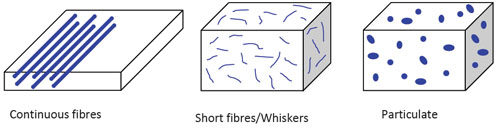
\includegraphics[scale=0.8]{pictures/Material-selection/composite-types}
  \begin{tikzpicture}
  \end{tikzpicture}
  \caption{Different types of engineering composites.}
\end{figure}

As common examples, engineering composites are combinations of strong fibers such as glass, carbon, and boron bonded together in a material like nylon, epoxy, or polyester. The constituents of a composite material are comprised of (1) matrix materials and (2) reinforcement materials. Various plastic resins and sometimes even metals are used as matrix materials. Common reinforcement materials are (a) glass, (b) carbon, (c) SiC, and (d) Kevlar (aramid), which can be in the form of (i) short fibers, (ii) long fibers, (iii) continuous fibers, (iv) randomly oriented fibers, (v) woven fibers (cloth), or (vi) particulates (fillers). Particulates (fillers) can act as reinforcement although they are usually added to a matrix to reduce costs or achieve specific material properties. Examples would be glass beads added to a thermoplastic matrix to reduce cost or mica added to a phenolic matrix to improve electrical properties and/or material processing. As the names suggest, reinforcement materials provide improved physical and mechanical properties—strength and stiffness—and the matrix material supports, surrounds and maintains the position of and transfers load to the reinforcement material.

Because reinforcing material is often made from fibers of larger pieces of the material, the composite benefits from the size effect. The fibers of smaller diameter have higher tensile strengths than the parent material. Glass, for example, has a relatively low tensile strength, yet the glass fiber has a much higher strength than glass in sheet form. The directionality and orientation of the composite material determines its properties and behavior. The orientation of reinforcement fibers within the composite such as (a) parallel, (b) woven, (c) random, (d) wound, and (e) angled can be used to take best advantage of the directional properties of the material. Where a ply (single layer) has strong directionality properties, structures of multiple plies or laminates are employed where each ply is arranged to provide improved strength and stiffness.

Glass fiber reinforcement improves the strength of plastics by a factor of two or more. At substantially increased cost, a further improvement is obtainable by carbon fiber reinforcement. These relatively new materials (with 10 to 40 percent carbon) have tensile strengths as high as 275 MPa. Compared to glass-reinforced resins, they have less mold shrinkage, lower coefficients of expansion, and improved creep resistance, wear resistance, and toughness. The new fiber-reinforced plastics are being increasingly used for machine and structural components requiring light weight and high strength-to-weight ratios.

Thermosetting plastics benefit similarly from glass reinforcement, the most commercially important being polyester and epoxy resins. In using tables giving properties of plastics, it is important as well to recall pitfalls in the use of such handbook data on the properties of materials. These pitfalls are particularly true for the data on plastics. Published values reflect values obtained from standardized molding conditions that are simple, economical, and readily reproduced. Strength values corresponding to actual molding conditions may differ significantly. Furthermore, temperature and rate of loading influence the strength of plastics to a greater extent than they do the strength of metals, thus requiring additional effort for the proper selection of a plastic.

In general, because of the influence of directionality of the composite material, a minimum of at least two Young’s moduli, a shear modulus, and a Poisson ratio are needed for the analysis of stiffness. Figure 2.3, 2.4, and 2.5 provide additional information for composite materials with respect to strength vs. modulus, strength vs. density, and strength vs. temperature, respectively. Types of composite materials identified include carbon-fiber-reinforced polymers (CFRP), glass-fiber-reinforced polymers (GFRP), SiC-reinforced aluminum (Al-SiC), and Kevlar-fiber-reinforced polymers (KFRP). Additional technical information including applications of polymer matrix composites (PMC), metal matrix composites (MMC) and ceramic matrix composites (CMC) is provided in references [17], [18], and [19]

\subsection{Fibers}

Fibers consist of thousands of filaments, each sufficiently small so that they can be manufactured using textile machines. The fibers are typically sold as as either

\begin{itemize}
\item Short fibers, with lengths of a few centimeters or millimeters are felts, mats, and short fibers used in injection molding.
\item Long fibers which can be cut during fabrication time are used as is or woven.
\end{itemize}

Main principal fiber materials are

\begin{enumerate}
\item Glass fiber: obtained by pulling glass (silicon + sodium carbonate and calcium carbonate) at $T > 1000^{\circ}$C through small orifices.
\item Kevlar fiber: This is an aramid fiber, yellowish in color. These are aromatic polyamides obained by synthesis at $-10^{\circ}$C, then fibrillated and drawn to obtain high modulus of elasticity.
\item Carbon fiber: filaments of polyacrilonitrile or pitch are oxidized at $T > 300^{\circ}$C, then heated further to $1500^{\circ}$C in a notrogen atmosphere. Then only the hexagonal carbon chains remain. High modulus of elasticity is obtained by drawing at high temperature.
\item Boron fiber: tungsten filament serves to catalize the reation between boron chloride and hidrogen at 1200$^{\circ}$C. The boron fiber obtained have a diameter of about 100 $\mu$m.
\item Silicon carbide: the principle of fabrication is analogous to that of boron fiber: chemical vapor deposition of methyl trichlorosilane mixed with hydrogen.
\end{enumerate}

\subsection{Matrix Materials}

The materials used as matrix in composite materials are

\begin{itemize}
\item Polymeric matrix: thermoplastic resins (polypropylene, polyphenylene sulfone, polyamide, etc.) and thermoset resins (polyesters, phenolics, melamines, silicones, and epoxies).
\item Mineral matrix: silicon carbide, carbon. They can be used at high temperatures.
\item Metallic matrix: aluminum alloys, titanium alloys.
\end{itemize}

\subsection{Properties of Composite Materials}

The characteristics of composite materials resulting from the combination of reinforcement and matrix depend on

\begin{itemize}
\item the proportions of reinforcements and matrix
\item the form of the reinforcement
\item the fabrication process
\end{itemize}

These characteristics maybe observed in ... {\color{Red}Figure...} which shows the tensile strength for different fiber fractions and different forms of reinforcement for the case of glass/resin composite, and {\color{Red}Figure 1.6} which gives an interesting view on the specific resistance of the principal composites as a function of temperature.

Other remarkable properties of these materials include the following:

\begin{itemize}
\item Composite materials \emph{do not yield} (their elastic limits correspond to the rupture limit).
\item Composite materials are very fatigue resistant.
\item Composite materials \emph{age} subject to humidity and heat.
\item Composite materials do not corrode.
\item Composite materials are not sensitive to common chemicals used in engines like crease, oils, paints, solvents. Paint thinners attact epoxy resins, however.
\item Composite materials have medium to low level impact resistance, inferior to that of metallic materails.
\item Composite materials have excellent fire resistance as compared with the light alloys with identical thicknesses. However, smokes from the combustion of certain metrices can be toxic.
\end{itemize}

Properties of some of the commonly used resins and reinforcements are listed in
\cref{tab: resin props} and \cref{tab: reinforcement props}.

\begin{table}[h]
  \centering
  \begin{tabular}{lcccccc}
    \toprule
          & $\rho$         & $E$ & $G$ & $\nu$ & $S_{ut}$ & Elongation \\
    Resins & {[}kg/m$^3${]} & {[}GPa{]} & {[}GPa{]} &       & {[}MPa{]}      & $E\%$ \\
    \midrule
    \multicolumn{7}{c}{\emph{Thermosets}} \\
    Epoxy         & 1200 & 4.5          & 1.6 & 0.4  & 130 & 2 (100$^{\circ}$C) \\
    Phenolic      & 1300 & 3.0          & 1.1 & 0.4  & 80  & 2.5 \\
    Polyester     & 1200 & 4.0          & 1.4 & 0.4  & 80  & 2.5 \\
    Polycarbonate & 1200 & 2.4          &     & 0.35 & 60  & \\
    Vinylester    & 1150 & 3.3          &     &      & 75  & 4 \\
    Silicone      & 1100 & 2.2          &     & 0.5  & 35  & \\
    Urethane      & 1100 & 0.7 - 7.0    &     &      & 30  & 100 \\
    Polyimide     & 1400 & 4.0 - 19     & 1.1 & 0.35 & 70  & 1 \\
    \multicolumn{7}{c}{\emph{Thermoplastics}} \\
    Polypropylene          & 900  & 1.2 & & 0.4  & 30  & 20 - 400 \\
    Polyphenylene sulfone  & 1300 & 4.0 & &      & 65  & 100 \\
    Polyamide              & 1100 & 2.0 & & 0.35 & 70  & 200 \\
    Polyether sulfone      & 1350 & 3.0 & &      & 85  & 60 \\
    Polyetherimide         & 1250 & 3.5 & &      & 105 & 60 \\
    Polyether-ether-ketone & 1300 & 4.0 & &      & 90  & 50 \\
    \bottomrule
  \end{tabular}
  \caption{Properties of commonly used resins \cite{gay2014composite}}
  \label{tab: resin props}
\end{table}

\begin{table}[h]
  \centering
  \begin{tabular}{lcccccc}
    \toprule
                   & $\rho$         & $E$ & $G$       & $\nu$ & $S_{ut}$  & Elongation \\
    Reinforcements & {[}kg/m$^3${]} & {[}GPa{]} & {[}GPa{]} &       & {[}GPa{]} & $E\%$ \\
    \midrule
    ``R'' glass                 & 2500 & 86  &     & 0.2  & 3.2 & 4 \\
    ``E'' glass                 & 2600 & 74  & 30  & 0.25 & 2.5 & 3.5 \\
    Kevlar 49                   & 1450 & 130 & 12  & 0.4  & 2.9 & 2.3 \\
    HT (high-strength) graphite & 1750 & 230 & 50  & 0.3  & 3.2 & 1.3 \\
    HM (high-modulus) graphite  & 1800 & 390 & 120 & 0.35 & 2.5 & 0.6 \\
    Boron                       & 2600 & 400 &     &      & 3.4 & 0.8 \\
    Aluminum                    & 3700 & 380 &     &      & 1.4 & 0.4 \\
    Aluminum silicate           & 2600 & 200 &     &      & 3.0 & 1.5 \\
    Silicon carbide             & 2550 & 200 &     &      & 2.8 & 1.3 \\
    Polyethylene                & 960  & 100 &     &      & 3.0 & \\
    \bottomrule
  \end{tabular}
  \caption{Properties of commonly used reinforcements \cite{gay2014composite}}
  \label{tab: reinforcement props}
\end{table}

\section{Engineering Material Selection Process}

The selection of materials and the processes used in manufacturing a machine component always influence one another, which in turns influences the cost of the component. This section introduces the student to a complex process of materials selection for machine components. Although actual material selection is based on experience and specific technical knowledge, this section attempts to provide a rational basis for the process.

During the design process, overall machine performance is established, after which components are selected and their specifications are developed to fit with the previously set machine performance. The material selection process typically takes place when the detailed dimensions of the components are determined.

The material selection process usually requires satisfying more than one constraint, for example, load and thermal or cost and power. This can be done by mapping the constraints to the material properties that influence those constraints. The constraints can then be transformed into the required ranges of material properties, which helps narrowing down the qualified materials. Cost and availability considerations are also added to finalize the group of candidate materials.

\subsection{Material Selection Factors}

Important material selection factors to fulfill design requirements are:
\begin{enumerate}
\item Availability: The availability of a material refer to the ease and cost of procuring the amount of material required for the component. The designer must also assess the risk of the availability and consider if there are any special treatments needed when obtaining and processing the material.
\item Cost: Cost should definitely be one of the first factors to be considered. However, actual material-related costs can vary depending on the design. These material-related costs are the raw material cost, cost of processing and manufacturing, cost of installation, and cost of operation and maintenance. It is also important to consider other lifecycle costs such as service life, transportation, recycling, and disposal.
\item Material Properties: The designer must understand the strengths and weaknesses of materials in consideration.
\item Manufacturing Processes: It is important to understand the links among chosen materials, the manufacturing process, and the material properties. Forming, joining, or fastening materials in certain ways limit the choice of materials; a given material may also limit the choice of manufacturing processes. And both the choice of materials and manufacturing processes will limit the range of obtainable material properties.
\item Formability and Joinability: A chosen material must be able to be formed into desired shape and/or join with other required components.
\item Finishing and Coatings: The choice of finishing or coating can be an inexpensive method to enhance material properties without switching to a stronger, more expensive material.
\end{enumerate}

\subsection{Materials Selection Charts}

Browsing through materials whose properties fit within the require ranges can be a daunting task. As such, Ashby’s materials selection charts, which graphically present material properties in a short and informative way, can be immensely helpful in facilitating the process of materials selection. It is important to note that the information contained in the charts is for rough calculations and not for final design. After a set of possible candidate materials have been selected, actual properties of selected materials should be used in the final design, followed by additional experimental verification and testing.

Some of the most useful charts for mechanical design are illustrated and discussed here.

\subsubsection{Strength-Stiffness Chart}

For design requirements that are controlled by elastic design or a ratio of strength versus Young’s modulus, the proper materials can be selected or compared by (1) energy storage per volume as in springs, $S^2/E = C$; (2) radius of bending as in elastic hinges, $S/E = C$; or (3) deflection under load as in diaphragm design, $S^{3/2}/E = C$. For example, if we want to maximize energy storage per volume before failure, we want to maximize the value of $S^2/E = C$. Without other design limitations, inspection of the chart shows that engineering ceramics have the highest allowable $S^2/E$, followed by elastomers, engineering alloys (steels), engineering composites, engineering polymers, woods, and polymer foams having decreased values

\begin{figure}[h]
  \centering
  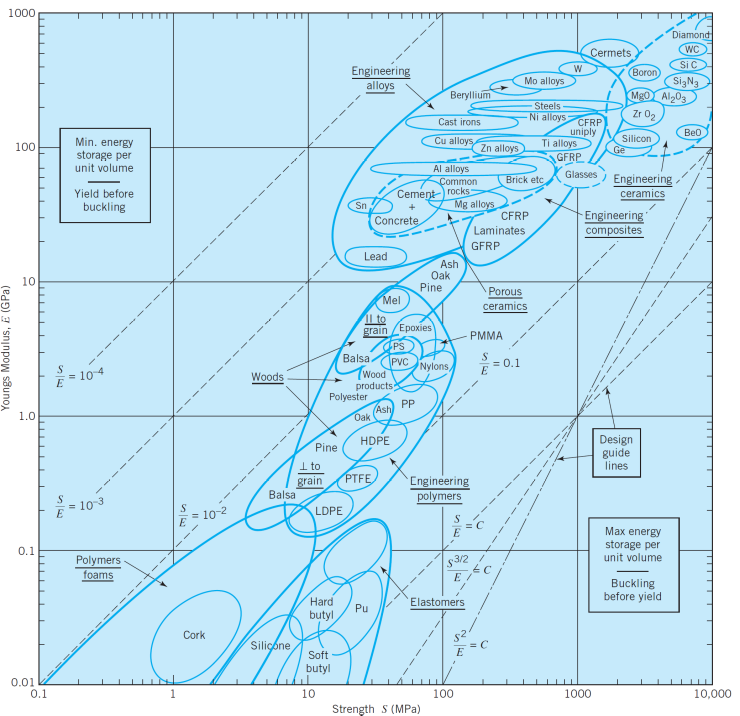
\includegraphics[scale=0.82]{pictures/Material-selection/strength-stiffness-diagram}
  \caption{Material strength, $S$, versus modulus, $E$, chart. \cite{ashby2010materials}}
  \label{fig: strength stiffness diagram}
\end{figure}

\subsubsection{Strength-Density Chart}
This chart is used for minimum weight design. By using the guidelines of constant $S/\rho = C$,
$S^{2/3}/\rho = C$, and $S^{1/2}/\rho = C$, a material that provide minimum weight design for rotating disks, beams, and plates, respectively can be determined.


\begin{figure}[h]
  \centering
  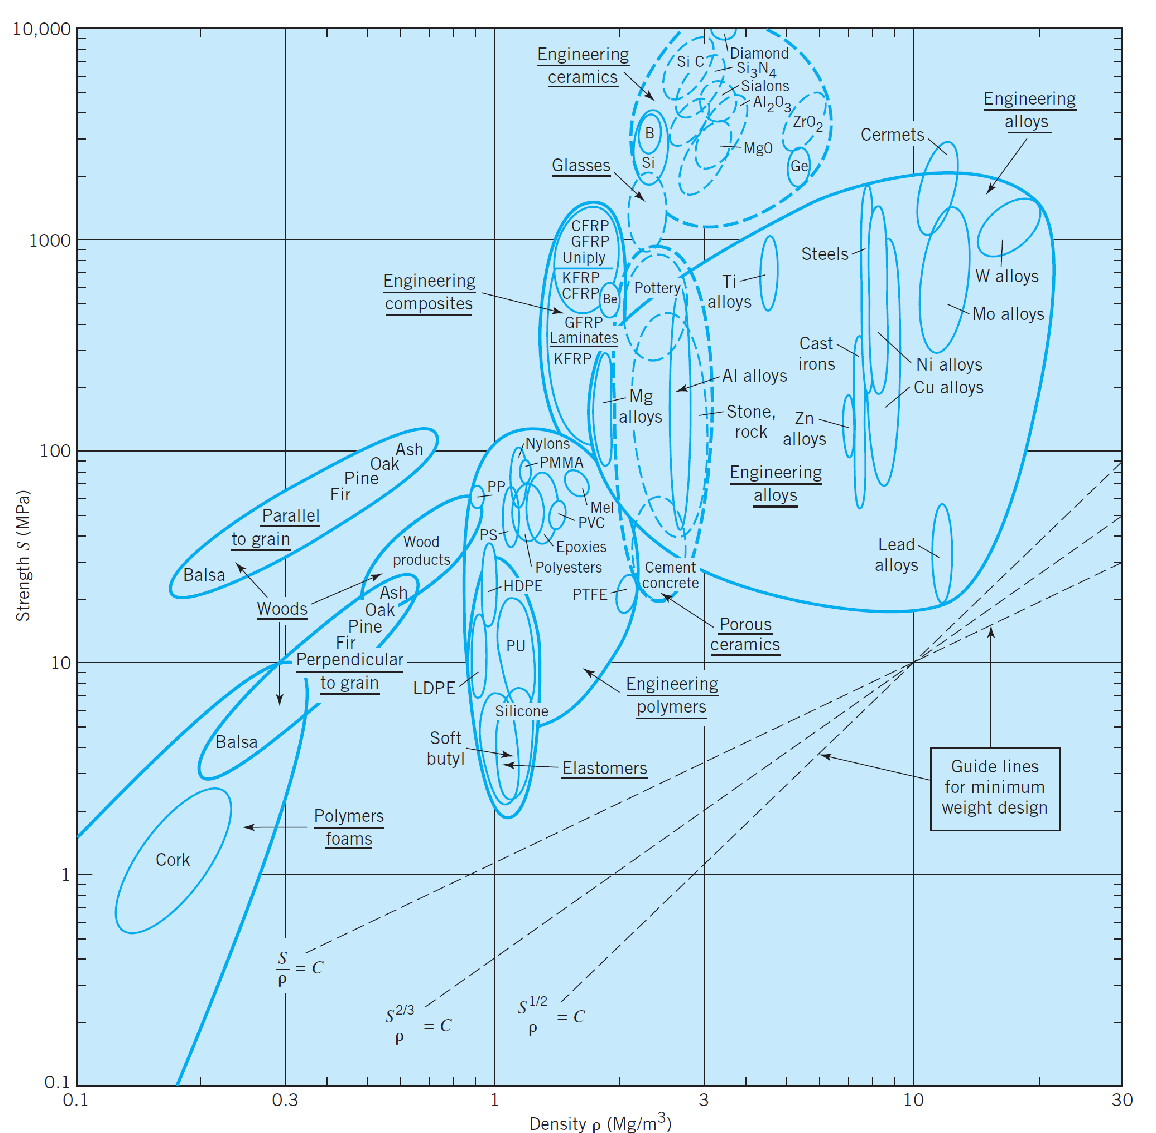
\includegraphics[scale=0.82]{pictures/Material-selection/strength-density-diagram}
  \caption{Material strength, $S$, versus density, $\rho$, chart. \cite{ashby2010materials}}
  \label{fig: strength density diagram}
\end{figure}

\subsubsection{Strength-Temperature Chart}

Strength-temperature relationship is used to determine suitable materials for designs that require strength at higher temperature. Notice that only ceramics have strength beyond 1000$^{\circ}$C, while alloys and polymers have strength up to only 800$^{\circ}$C and 300$^{\circ}$C, respectively.

\begin{figure}[h]
  \centering
  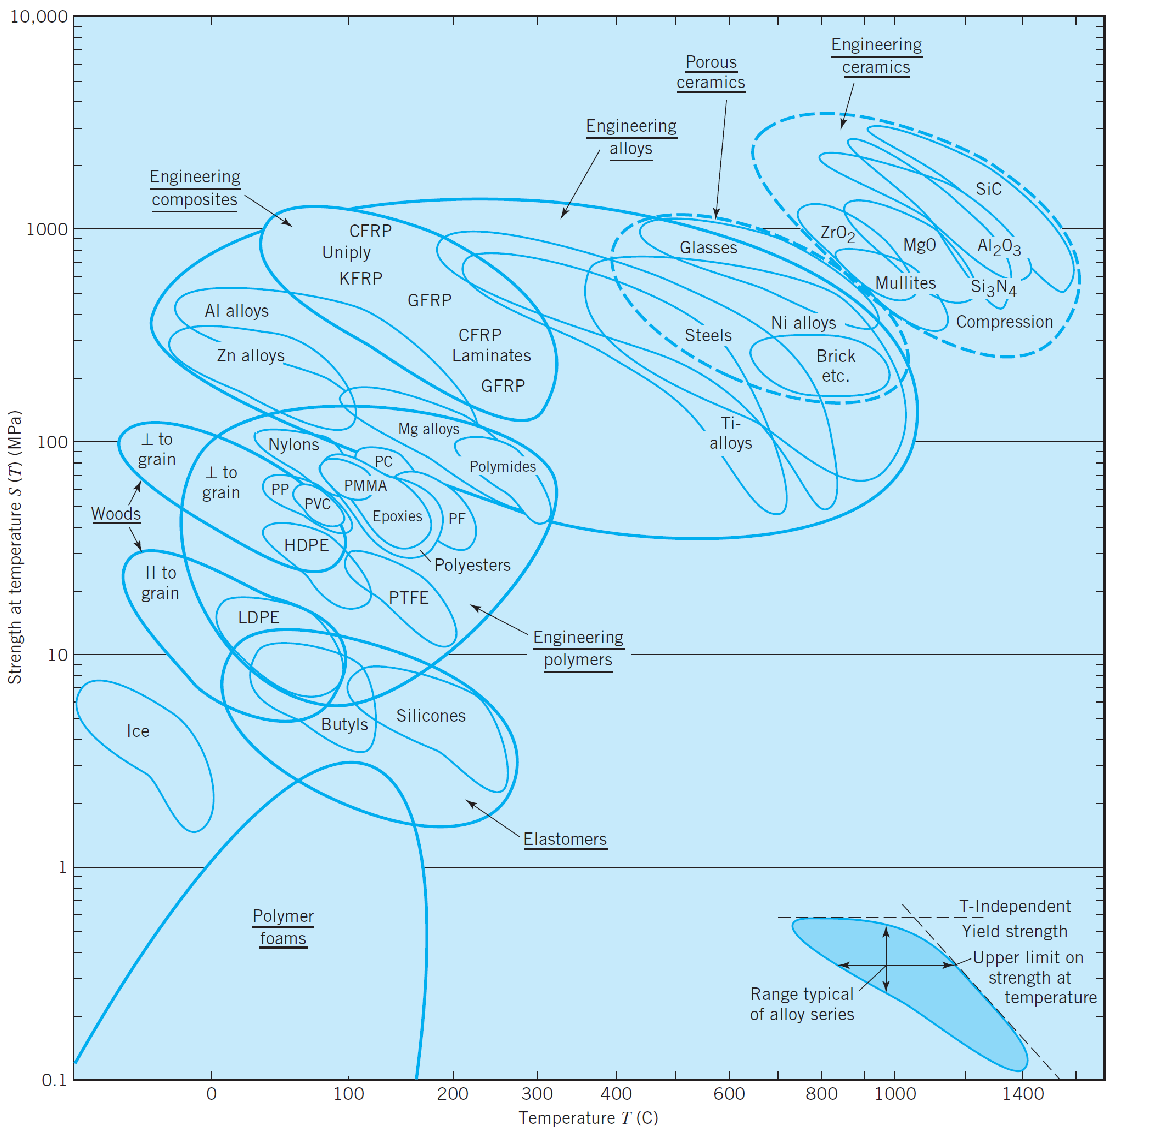
\includegraphics[scale=0.82]{pictures/Material-selection/strength-temperature-diagram}
  \caption{Material strength at different temperatures, $S(T)$, versus temperature, $T$, chart. \cite{ashby2010materials}}
  \label{fig: strength temperature diagram}
\end{figure}

\begin{example} Material selection for a gas turbine transmission shaft.

  An engineer is aiming to design a new transmission shaft for a luxury car. He wants the shaft to be as light as possible and to withstand the temperature of at least 300 C. Cost is not a main concern.

\end{example}
\begin{solution}
  There are obviously two criteria for consideration here. We will first tackle the temperature limit.

  In order for the shaft to still operate above 300 C, the shaft \emph{must} have strength above that temperature. This is where the strength-temperature chart is very useful.

  According to \cref{fig: strength temperature diagram}, we can draw a vertical line at 300 C. Materials that fall to the left side do not qualify as they do not possess sufficient strength above 300 C. That means all engineering composites, plastics, foams, along with aluminum, zinc, and magnesium alloys do not pass this requirement.

  For the minimum weight design, we refer to the strength-density chart. For shaft, the index $S^{1/2}/\rho$ is used to determine a proper material. The material (or group of materials) with the highest index will yield the minimum weight for a given torque requirement. From \cref{fig: strength density diagram}, the possible candidates are metal alloys. Combining this with the elimination we have made for the temperature requirement, the qualified materials are steels, titanium alloys, and Ni alloys. 

\end{solution}
\subsection{Material Selection Procedure}

Just like mechanical design problems, material selection tends to involve making decisions with neither complete nor accurate information about the functional requirements of the design. A simple methodology for materials selection is based on the performance, the importance, and the availability and final cost of the component.

Though the actual materials selection process can be iterative, requiring rethinking and decision-changing, when the designer has a description of the part, the typical selection process typically follows this path:

\begin{enumerate}

\item \emph{Establish required service performances}: Determine the operational conditions of the component, and translate those conditions into related material properties. For example, a beam that is to withstand repeated loadings at high temperature will require a different material than the one to withstand a static loading at room temperature.

\item \emph{Select a suitable material}: After the required performances and corresponding material properties have been identified, the designer can employ material selection charts to help screen suitable materials. Once the first round of suitable materials are obtained, reconsider formability, availability, cost, and other critical properties to obtain final candidates

\item \emph{Make a final evaluation}: Select the best material for the application. ‘Best’ is the material with the best value, defined as the ratio of overall performance over total cost, or as the material selection index (SI) where

  $$ SI = \frac{(\text{availability})(\text{performance})}{\text{total cost}} $$

\item \emph{Test, a lot of tests}: Perform test of the chosen material in operating conditions. Determine if an extensive testing of the final product is required. Reevaluate the risk and uncertainty of chosen material, for example, cost of product failure.

\end{enumerate}

\section*{Summary}

Material selection process is as challenging as other mechanical design processes. It involves analysis of the requirements, identification of materials, evaluation of candidate materials, and testing and verification. The important step is the translation of key functional requirements to required material properties, but also the inclusion of risk, economic, and process analysis.

\section*{Exercises}

\begin{exercises}

  \exercise Choose a proper plastic for a 2-liter cylindrical water container so that the final wall thickness will be no larger than 1 mm.

  \exercise Explain the reason steel-reinforced concrete is very strong.

  \exercise Why do racing cars employ carbon fiber reinforced polymer (CFRP) for their bodies rather than high strength steel even though CFRP is not as strong and more expensive?

  \exercise Select a proper material for an engine shaft. It should be able to withstand the torque of at least 200 N-m and not weigh more than 5 kg.

  \exercise Select a proper bolt material for a steel bolt so that the weight is minimized. Its ultimate tensile strength should be at least 400 MPa.

\end{exercises}

%%%%%%%%%%%%%%%%%%%%%%%%%%%%%%%%%%%%%%%%%%%%%%%%%%%%%%%%%%%%%%%%%%%%%%%%%%%%%%%%%%%%%%%%%%%%%%%%%%%%%%%%%%%%%%%%%%%%%%%%%%%%%%%%%%%%%%%%%%%%%%%%%%%%%%%%%%%%%%%%%%%%%%%%%%%%%%%%%%%%%%%%%%%%%%%%%%%%%%%%%%%%%%%%%%%%%%%%%%%%%%%%%

 
\chapter{Static Body Load Analysis}

In this chapter, topics covered in Mechanics of Materials that are directly related to Mechanical Design are reviewed. Mechanics of Materials is an important building block on which Mechanical Design is built upon; an engineer cannot effectively and properly design a component without understanding the type of loadings, supports, and stresses applied to the part.

\section{Stress, strain, and stress-strain relationship}

In engineering, the deformation of a body is specified using the concept of normal and shear strain. We will look at how stress deforms a body and how the deformation is quantified.

When a force is applied to a body, it will cause a body to change shape and size. These changes are called deformation. Note that deformation may not be uniform throughout the body. For example, one part of the body may contract while the other may expand.

The main interest in engineering mechanics of solids is to study the internal resistance of a body under externally applied forces. In earlier statics or dynamics courses, we study the effect of forces on rigid bodies. We may study how they move or how the forces distribute among many members of a structure, but we never study how the force affects each member. In reality, most bodies are deformable, the degrees of which depends on their material properties. In this case, we can still use the equation of equilibrium to determine the internal force acting inside the body.

$$ \sum F = 0 $$
$$ \sum M = 0 $$

\subsection{Concepts of Load}

Considering a surface cutting through the body, there can be 2 types of forces and 2 types of moments acting on the surface

\begin{itemize}
\item Normal force ($F$) acts perpendicular to the surface. This force is developed when there is an external loads pushing or pulling on the surface of the body.
\item Shear force ($V$) acts in the plane of the surface. It developed when the external forces tends to cause the surface to slide sideways.
\item Torsional moment or torque ($T$) is developed when the loads tend to twist the segment with respect to another.
\item Bending moment ($M$) is developed when the loads tend to bend the body about an axis lying within the plane of the surface.
\end{itemize}

\subsection{Definition of Stress}

By definition, stress is the force per unit cross sectional area that it is acting upon. There are two types of stress, depending on the direction the force is acting on the surface

\begin{enumerate}

\item Normal stress: force per unit area acting normal to the surface. It can be expressed mathematically as

\begin{equation}
\sigma  = \mathop {\lim }\limits_{A \to 0} \frac{F}{A}
\end{equation}

\item Shear stress: force per unit area acting tangent to the surface. This component can be expressed mathematically as

  \begin{equation}
    \tau  = \mathop {\lim }\limits_{A \to 0} \frac{V}{A}
  \end{equation}
\end{enumerate}

In the case of shear stress, we can further specify the direction of stress into rectangular components using $x$, $y$, $z$ coordinate axes, with $x$ and $y$ axes in the direction of the in-plane surface and $z$ axis normal to the surface. We can now express the normal stress components as

\begin{equation}
  \sigma _{zz} = \sigma _z = \mathop {\lim }\limits_{A \to 0} \frac{F_z}{A}
\end{equation}

and the two shear stress components as

\begin{equation}
  \arraycolsep=1.4pt\def\arraystretch{2.2}
  \begin{array}{l}
    \tau _{zx} = \mathop {\lim }\limits_{A \to 0} \dfrac{F_x}{A} \\
    \tau _{zy} = \mathop {\lim }\limits_{A \to 0} \dfrac{F_y}{A}
  \end{array}
\end{equation}

\subsection{Equilibrium Requirement}

Consider an infinitesimal cubic element, illustrated in \cref{fig: 3d-stress-element}, with external forces applied, each of the six faces of the cube will have three components of stress acting on it. If the stress around the point is constant, then we can use equilibrium equation to relate some of the stress components.

\begin{figure}[h]
  \centering
  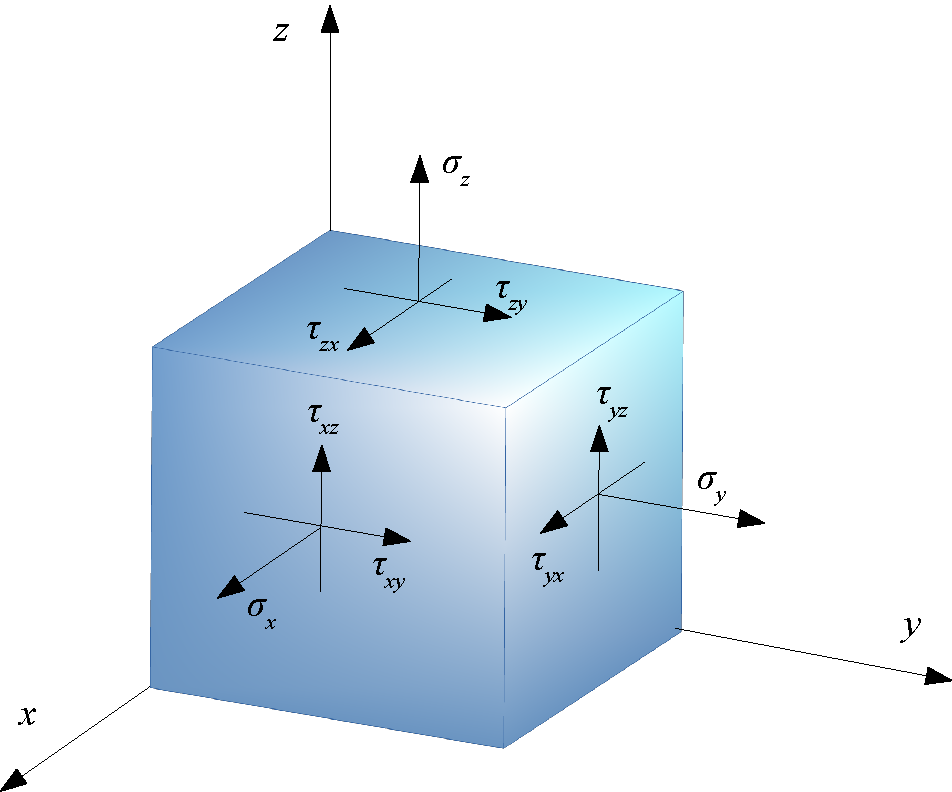
\includegraphics[scale=0.6]{pictures/Static-body-load-analysis/3d-element-stress}
  \caption{Stresses on a three-dimensional element when considering a static equilibrium}
  \label{fig: 3d-stress-element}
\end{figure}
  
\subsubsection{Normal Stress Components}

If we apply the equation of force equilibrium in the $x$ direction, then

\begin{equation}
  \arraycolsep=1.4pt\def\arraystretch{1.5}
  \begin{array}{c}
    \sigma _x(\Delta y\Delta z) + \sigma_x'(\Delta y\Delta z) = 0\\
    \sigma _x =  - \sigma_x'
  \end{array}
\end{equation}

We can similarly prove that $\sigma_y = \sigma_{y’}$ and $\sigma_z = \sigma_z’$. Therefore, for a constant state of stress, each of the three normal stress components must be equal in magnitude but opposite in direction.

\subsubsection{Shear Stress Components}

In similar fashion, the shear stresses on opposite faces are of the same magnitude but in opposite direction.
The force equilibrium in the $x$ direction gives

\begin{equation}
  \arraycolsep=1.4pt\def\arraystretch{1.5}
  \begin{array}{c}
    \tau _{yx}(\Delta y\Delta z) + \tau_{yx}'(\Delta y\Delta z) = 0\\
    \tau _{yx} =  - \tau_{yx}'
  \end{array}
\end{equation}

If we consider a pair of shear stresses loading on the element, the moment equilibrium about the z direction gives

\begin{equation}
  \arraycolsep=1.4pt\def\arraystretch{1.5}
  \begin{array}{c}
    \tau _{xy}(\Delta y\Delta z)\Delta x - \tau _{yx}(\Delta x\Delta z)\Delta y = 0\\
    \tau _{xy} = \tau _{yx}
  \end{array}
\end{equation}

\subsection{Deformation and Strain}

In order to describe deformation by changes in the length or by the changes in angles of the element, we will need to develop the concept of strain. As in stresses, there are two types of strain.

\subsubsection{Normal strain}

The change in the length of a line segment per unit length, whether elongation or contraction, is called normal strain. For example, consider the line AB which is contained within an undeformed body with length $s$. During its deformation, points A and B move to point A’ and B’ and the line becomes a curve having the length $s’$. The average normal strain becomes

\begin{equation}
  \varepsilon _{avg} = \frac{s' - s}{s}
\end{equation}

If the normal strain is known, we can use this equation to find the final length of the line segment after it is deformed. We have

\begin{equation}
  s' = (1 + \varepsilon_{avg})s
\end{equation}

Therefore, strain is positive when the line elongates and is negative when the line contracts.

\subsubsection{Shear Strain}

The change in angle that occurs between two line segments that were originally perpendicular is referred to as shear strain. This angle is denoted by and is measured in radians. Consider the same cubic element with shear stress couple applied in the $xy$-plane. The angle made by the original $x$ and $y$ axes is $90^{\circ}$. After the deformation, the angle is changed by $\theta$. The shear strain in the plane, $\gamma_{xy}$, can be defined as 

\begin{figure}
  \centering
  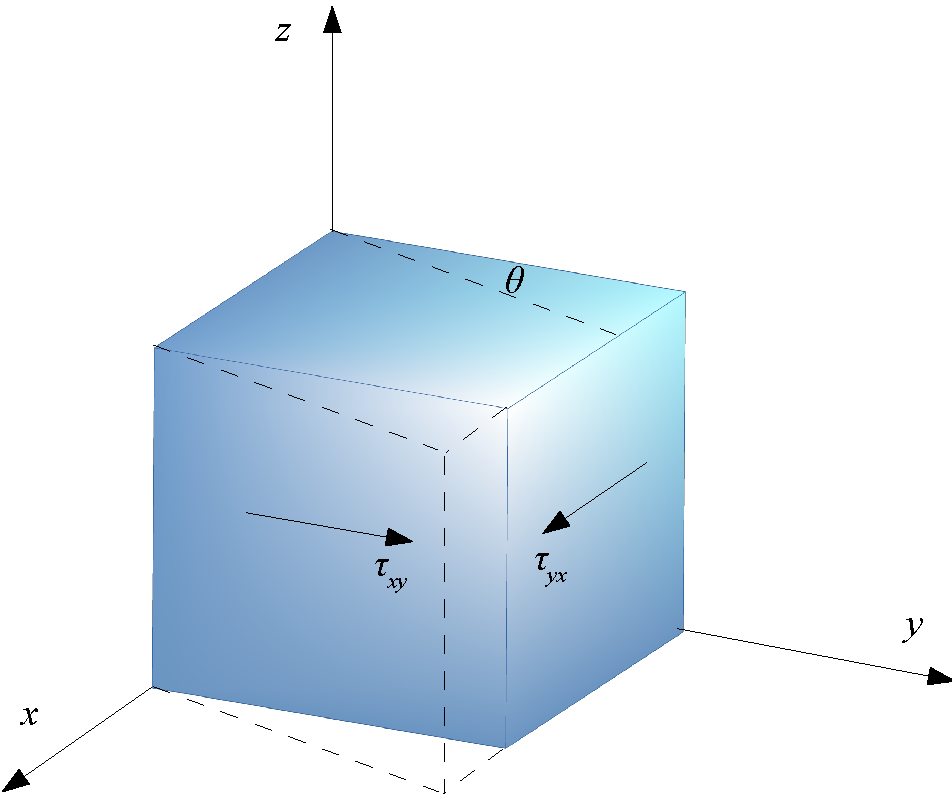
\includegraphics[scale=0.6]{pictures/Static-body-load-analysis/3d-shear-deformation}
  \caption{3-dimensional element under shear deformation.}
  \label{fig: 3d shear deformation}
\end{figure}

\begin{equation}
  \gamma _{xy} = \mathop {\lim }\limits_{y \to 0} \frac{dx}{y} = \tan \theta  \approx \theta
\end{equation}
 
\subsubsection{Cartesian Strain Components}

Using the above definition of normal and shear strains, we will now show how it can be used to describe the deformation in a body. Consider an infinitesimal element of dimension that is located near a point in the body. The deformed shape of the element is a parallelepiped, assuming that very small line segments will remain relatively straight after the deformation. The approximate lengths of the sides of the parallelepiped are  $(1 + \varepsilon_x)\Delta x$, $(1 + \varepsilon_y)\Delta y$, and $(1 + \varepsilon_z)\Delta z$ and the approximate angles between the sides are $(\pi /2) - \gamma_{xy}$, $(\pi /2) - \gamma_{yz}$, and $(\pi /2) - \gamma _{zx}$. Notice that the normal strains cause a change in the volume of the element, while the shear strains cause a change in its shape.

\subsection{Hooke’s Law in One Dimension}

Since the stress-strain relationship for most engineering materials exhibit a linear relationship between stress and strain within the elastic regime, an increase in stress causes a proportional increase in strain. This fact was discovered by Robert Hooke in 1676 and is known as Hooke’s law. It can be expressed mathematically as

\begin{equation}
  \sigma  = E\varepsilon
\end{equation}

Here $E$ represents the constant of proportionality, which is called the modulus of elasticity or Young’s modulus.

\subsection{Poisson’s Ratio}

When a deformable body is subjected to an axial tensile force, not only does it elongate but it also contracts laterally. A French scientist S. D. Poisson found that the ratio between lateral and the longitudinal strains are always constant in the elastic regime. This constant is referred to as Poisson’s ratio, $\nu$, defined as

\begin{figure}[h]
  \centering
  \begin{tikzpicture}
    \node [draw, rectangle, minimum height=2cm, minimum width=2cm, fill=LightBlue, inner sep=0](A){};
    \node [draw, dashed, rectangle, minimum height=1.8cm, minimum width=2.4cm, fill=LightBlue, fill opacity=0.5, inner sep=0](B){};
    \foreach \x in {1,...,8} {
      \draw [->] (1.2, 0.9-0.2*\x) --++ (0:0.5);
      \draw [->] (-1.2, 0.9-0.2*\x) --++ (180:0.5);
    }

    \node at (A.west) [yshift=-1.5cm](C){};
    \node at (A.east) [yshift=-1.5cm](D){};

    \node at (B.west) [yshift=-2cm](E){};
    \node at (B.east) [yshift=-2cm](F){};

    \draw [|<->|] (C.center) -- (D.center) node[midway,above]{$L$};
    \draw [|<->|] (E.center) -- (F.center) node[midway,below]{$L(1+\varepsilon_{long})$};

    \node at (A.north) [xshift=-2cm](G){};
    \node at (A.south) [xshift=-2cm](H){};

    \node at (B.north) [xshift=-3cm](I){};
    \node at (B.south) [xshift=-3cm](J){};

    \draw [|<->|] (G.center) -- (H.center) node[midway,left]{$L$};
    \draw [|<->|] (I.center) -- (J.center) node[text width=2.7cm,midway,left]{$L(1+\varepsilon_{lat})$ \\
      $= L(1-\nu\varepsilon_{long})$};
  \end{tikzpicture}
\end{figure}

\begin{equation}
  \nu  =  - \frac{\varepsilon _{lat}}{\varepsilon _{long}}
\end{equation}
  
Notice the negative sign here since longitudinal elongation causes lateral contraction, and vice versa. Poisson’s ratio has no unit, or dimensionless, and for most nonporous material it has a value between 0.25 and 0.33.

\subsection{Shear stress-shear strain relationship}

Much like the way there is a relationship between normal stress and normal strain in most engineering materials, shear stress and shear strain are also related linearly by the equation

\begin{equation}
  \tau  = G\gamma
\end{equation}

$G$ is called the shear modulus of elasticity and has the same unit as Young’s modulus

\section{Thermal effect}

A change in temperature can cause a material to change its dimensions. If the temperature increases, generally a material expands, whereas if the temperature decreases, the material will contract. Ordinarily this expansion or contraction is linearly related to the temperature increase or decrease that occurs. If the material is homogeneous and isotropic, it has been found that the deformation of a part having length $L$ can be calculated using the formula

\begin{equation}
  \delta _T = \alpha \Delta TL
\end{equation}

where $\alpha$ is a property of a material, referred to as the linear coefficient of thermal expansion, measuring strain per degree temperature, $\Delta T$ is the change in temperature of the part, $L$ is the original length of the member, and $\delta T$ is the change in length of the part.

However, if the change in temperature varies throughout the length of the part so that or if varies along the length, then the equation becomes

\begin{equation}
  \delta _T = \int_0^L \alpha \Delta Tdx
\end{equation}

Without any constraint, the change in length of the part can be computed using the given equations. However, if the expansion or contraction is restrained by supports, it will produce thermal stress in the part because it cannot deform freely.
  
\begin{example}
  
  A rubber bar of original length $L$ is stretched and glued between two walls. After that the bar is heated from its initial temperature $T_0$ to $T$ at which point there is no longer any remaining stress inside the bar. What is the distance between the two walls? Assume the material has modulus of elasticity $E$ and coefficient of thermal expansion $\alpha$.
  
  \begin{figure}[H]
    \centering
    \begin{tikzpicture}
      \path[fill=white] (-5,-2) rectangle (5,2);
      \node [draw, fill=SkyBlue, minimum height=4mm, minimum width=8cm](beam){};
      \node at (beam.west) [anchor=east, draw, fill=LightGrey, pattern=north west lines, minimum height=2cm, minimum width=5mm](left){};
      \node at (beam.east) [anchor=west, draw, fill=LightGrey, pattern=north west lines, minimum height=2cm, minimum width=5mm](right){};
      \draw[|<->|] (left.south east) ++ (-90:0.5) --++ (0:8) node[midway, fill=white]{$L$};
      \draw (0,0.5) node{$T_0 \rightarrow T$};
    \end{tikzpicture}
  \end{figure}
  
\end{example}
\begin{solution}
  Assume the distance between the two walls is $D$. Since there is no stress in the bar, which means thermal expansion has caused the bar to expand from original length $L$ to length $D$. Therefore,
  
\[\begin{gathered}
  D - L = \alpha (T - T_0)L \hfill \\
  D = L[1 + \alpha (T - T_0)] \hfill \\ 
\end{gathered}\]
	
\end{solution}

\begin{example} Heated Steel Bar

  A 50-cm long steel cylindrical bar is heated on one end by a bunsen burner until it reaches a steady state. Initially, the bar has a constant temperature of 20 $^{\circ}$C. Due to the effects of convection and conduction, the temperature profile of the steel along its length is dependent on the distance from the burner $x$

  \begin{figure}[H]
    \centering
    \begin{tikzpicture}
      \node [fill=white, minimum height=4cm, minimum width=12cm]{};
      \node [draw, rectangle, left color=LightSkyBlue, right color=Red!40, middle color=Yellow!30, minimum height=5mm, minimum width=8cm](bar){};
      \node at (bar.south east)[anchor=north, draw, ellipse, minimum height=1cm, minimum width=4mm, fill=Red](outflame){};
      \node at (outflame.south)[anchor=south, draw, ellipse, minimum height=6mm, minimum width=2mm, fill=Yellow](inflame){};
      \node at (outflame.south)[anchor=north, draw, rectangle, left color=Grey, right color=Grey, middle color=LightGrey, minimum height=0.5cm, minimum width=2cm](burner){};
      \node at (bar.north) [above]{$T(x) =  100x^2 - 200 x + 400$};
      \draw [->] (bar.north east) ++ (90:0.3) --++ (180:1) node[midway, fill=White]{$x$}; 
    \end{tikzpicture}
  \end{figure}
  
  Determine the change in length of the beam at steady state, given that the steel bar has $\alpha = 13 \times 10^{-6}$ /$^{\circ}$C
\end{example}
\begin{solution}

  Since the temperature is given as a function, we simply need to integrate the expression to determine the change in length

  \begin{align*}
    \delta_T &= \int_0^L \alpha \Delta T dx \\
             &= \int_0^{0.5} 13 \times 10^{-6} (100x^2 - 200x + 400 - 20) dx \\
             &= 13 \times 10^{-6} \left. \left( \frac{100}{3} x^3 - 100 x^2 + 380 x \right) \right|_0^{0.5} \\
             &= 2.2 \times 10^{-3} \text{ m}
  \end{align*}
\end{solution}
  
\section{Axially loaded members}

The main concern here will be the stresses and associated deformations due to axial loadings. It is often necessary to determine not only the stresses in an axially loaded member but the deflections as well, The latter, for example, may have to be kept within limits so that certain clearances are maintained.
This section deals with the elongation or contraction of slender homogeneous members under axial loading. The axial stress in these cases is assumed not to exceed the yield strength of the material. The definition of normal stress, normal strain, and the relationship between the two given by Hooke’s law are employed.

\subsection{Prismatic bars}

When determining the changes in length of axially loaded members, it is convenient to begin with a coil spring. When a load is applied along the axis of a spring, the spring gets shorter or longer depending on the direction of the load.

Similarly, in the case of axially loaded members, they elongate or shorten depend on the direction of the load. If the load acts toward the member, it is in compression. If the load acts away from the member, it is in tension. It is also important to note its natural length L, also called its free length or relaxed length. Once the member is loaded, supposedly in tension, it will lengthen by an amount $\delta$ and its final length becomes $L + \delta$. If the material of the spring is linearly elastic, the load and elongation will be proportional, following Hooke’s law that

\begin{figure}[h]
  \centering
  \begin{tikzpicture}
    \draw[fill=Grey] (-1,-1) rectangle (0,2);
    \draw[fill=SkyBlue] (0,0) rectangle (5,1);
    \draw[fill=SkyBlue, fill opacity=0.5, dashed] (0,0) rectangle (5.5,1);
    \draw[->,ultra thick] (5.5,0.5) -- (6.5,0.5) node[right]{$P$};
    \draw[<->] (0,-0.5) -- (2.5,-0.5) node[above]{$L$} -- (5,-0.5);
    \draw[<->] (5,-0.5)-- (5.25,-0.5) node[above]{$\delta$} -- (5.5,-0.5);
    \draw[<->] (1,0) -- (1, 0.5) node[right]{$A$} -- (1,1);
  \end{tikzpicture}
  \caption{Deformation of a axially loaded constant cross-sectioned member.}
\end{figure}

\[\arraycolsep=1.4pt\def\arraystretch{2.2}
  \begin{array}{l}
    \sigma  = \dfrac{P}{A}\\
    \varepsilon  = \dfrac{\delta }{L}\\
    \sigma  = E\varepsilon 
  \end{array}\]

And therefore we can derive for these relationships that

\begin{equation}
  \delta  = \frac{PL}{AE}
\end{equation}

This equation shows that the elongation is directly proportional to the load $P$ and the member length $L$, and inversely proportional to the modulus of elasticity $E$ and the cross-sectional area $A$. This equation works assuming that the bar has a uniform cross section.

\subsection{Nonprismatic bars}

However, if the bar is loaded by different axial loads, bar made of different materials, or its cross sectional area varies throughout its length, the stress throughout the bar varies. To solve for the total change in length of this type of problem, we must 1) identify the segments of the bar, 2) determine the axial forces in the segments from the free body diagrams, 3) applies the equation to all segments. The total change in length is the sum of the changes in length in all segments, or

\begin{figure}[h]
  \centering
  \begin{tikzpicture}
    %members
    \draw[fill=SkyBlue] (0,0) rectangle (3,1) ;
    \draw[fill=SkyBlue] (3,-0.5) rectangle (5,1.5);
    \draw[fill=SkyBlue] (5,-0.25) rectangle (7.5,1.25);
    % extended members
    \draw[fill=SkyBlue, fill opacity=0.5, dashed] (0,0) rectangle (3.1,1) ;
    \draw[fill=SkyBlue, fill opacity=0.5, dashed] (3.1,-0.5) rectangle (5.2,1.5);
    \draw[fill=SkyBlue, fill opacity=0.5, dashed] (5.2,-0.25) rectangle (7.8,1.25);
    %force
    \draw[->,ultra thick] (7.8,0.5) -- (8.8,0.5) node[right]{$P$};
    \draw[<-,ultra thick] (-1,0.5) node[left]{$P$} -- (0,0.5);
    %lengths
    \draw[|<->|] (0,-1.5) -- (1.5,-1.5) node[above]{$L_1$} -- (3,-1.5);
    \draw[|<->|] (3,-1.5)-- (4,-1.5) node[above]{$L_2$} -- (5,-1.5);
    \draw[|<->|] (5,-1.5)-- (6.25,-1.5) node[above]{$L_3$} -- (7.5,-1.5);
  %areas
    \draw[<->] (1,0) -- (1, 0.5) node[right]{$A_1$} -- (1,1);
    \draw[<->] (4,-0.5) -- (4, 0.5) node[right]{$A_2$} -- (4,1.5);
    \draw[<->] (6,-0.25) -- (6, 0.5) node[right]{$A_3$} -- (6,1.25);
  \end{tikzpicture}
  \caption{Nonprismatic bar with segments of constant cross sections under axial load.}
\end{figure}

\begin{equation}
  \delta  = \sum\limits_{i = 1}^n \frac{P_iL_i}{E_iA_i}
\end{equation}

In which $i$ is the index of various segments of the bar and $n$ is the total number of segments. Note that the force $P_i$ is the internal axial force in the segment $i$, not the external force.

Some other times, the axial force $P$ and the cross-sectional area $A$ vary continuously along the axis of a bar. In this case, instead of using an algebraic sum, we must integrate the small changes along the length of a bar to calculate the total change in length.

Consider a small slither of the bar that has length $dx$ and cross-sectional area $A(x)$ locating at a distance $x$ from one end of the bar. Assume the internal force acting on the slither of the bar follows the function $P(x)$. The change in length of the slither is simply

\begin{figure}[h]
  \centering
  \begin{tikzpicture}
    \draw[fill=Grey] (-1,-1) rectangle (0,2);
    \draw[fill=SkyBlue] (0,-0.5) -- (5,0) -- (5,1) -- (0,1.5);
    \draw[fill=SkyBlue, fill opacity=0.5, dashed] (0,-0.5) -- (5.5,0) -- (5.5,1) -- (0,1.5);
    \draw[->,ultra thick] (5.5,0.5) -- (6.5,0.5) node[right]{$P$};
    \draw[<->] (0,-1) -- (2.5,-1) node[above]{$L$} -- (5,-1);
    \draw[<->] (5,-1)-- (5.25,-1) node[above]{$\delta$} -- (5.5,-1);
    \draw[<->] (1,-0.4) -- (1, 0.5) node[right]{$A(x)$} -- (1,1.4);

    \draw[fill=SkyBlue] (8,-0.4) rectangle (8.2,1.4);
    \draw[fill=SkyBlue, fill opacity=0.5, dashed] (8,-0.4) rectangle (8.3,1.4);
    \draw[->|] (7.8,-1) node[left]{$dx$}  to (8,-1);
    \draw[|<-] (8.2,-1) to (8.4,-1);
    \draw[->|] (8,-0.7) to (8.2,-0.7);
    \draw[|<-] (8.3,-0.7) to (8.5,-0.7) node[right]{$d\delta$};
  \end{tikzpicture}
  \caption{Deformation of an axially loaded continuously variable cross-sectioned member.}
\end{figure}

  \[d\delta  = \frac{P(x)dx}{EA(x)}\]

And the total elongation of the entire bar is

\begin{equation}
  \delta  = \int_0^L {d\delta }  = \int_0^L \frac{P(x)dx}{EA(x)}
\end{equation}


\section{Torsion}

Torsion is a twist of a straight bar when loaded by moments that tend to produce rotation about the longitudinal axis of the bar.

The convention for the moment, also called twisting moment, follows the right hand rule. In this chapter, we begin by developing formulas for the deformations and stresses in circular bars under torsion. We then analyze the rotating shafts and determine the power they transmit. Finally, we cover several additional topics related to torsion such as statically indeterminate members, strain energy, thin-walled tubes, and nonlinear torsion behavior.

\subsection{Simple torsion}

Simple torsion is the case where the cross-sectional area and the torque throughout the length of the material are constant. The understanding of simple torsion and its conditions can be applied to other more complex torsion in upcoming sections.

When a circular bar is twisted by torques $T$ at the ends, every cross section of the bar is still identical and is subjected to the same internal torque $T$, we say that the bar is in pure torsion. From consideration of symmetry, it can be proved that cross sections of the bar do not change in shape as they rotate about the longitudinal axis. Furthermore, if the angle of rotation between one end of the bar and the other is small, neither the length of the bar nor its radius will change.

\begin{figure}[h]
  \centering
  \begin{tikzpicture}
    \draw [->, thick] (0,0) --++ (90:3) node[right]{$z$};
    \node at (0,0) [anchor=west, xshift=-8mm, draw, top color=LightSkyBlue, bottom color=LightSkyBlue, middle color=LightSkyBlue!40, cylinder, minimum height=8cm, minimum width=3cm, inner sep=0.8cm](cyl){};
    \draw [->>, ultra thick] (cyl.east) ++ (180:0.8) node(O){} --++ (0:2) node[above]{$T$};
    \draw [very thin] (O.center) --++ (120:1.19) --++ (180:6.4) node(A){};
    \draw [very thin] (O.center) --++ (200:0.86) node(B){};
    \draw [very thin, dashed] (B.center) -- (A.center);
    \node at (O.center) [left, yshift=1mm, xshift=-1mm] {$\phi$};
  \end{tikzpicture}
  % 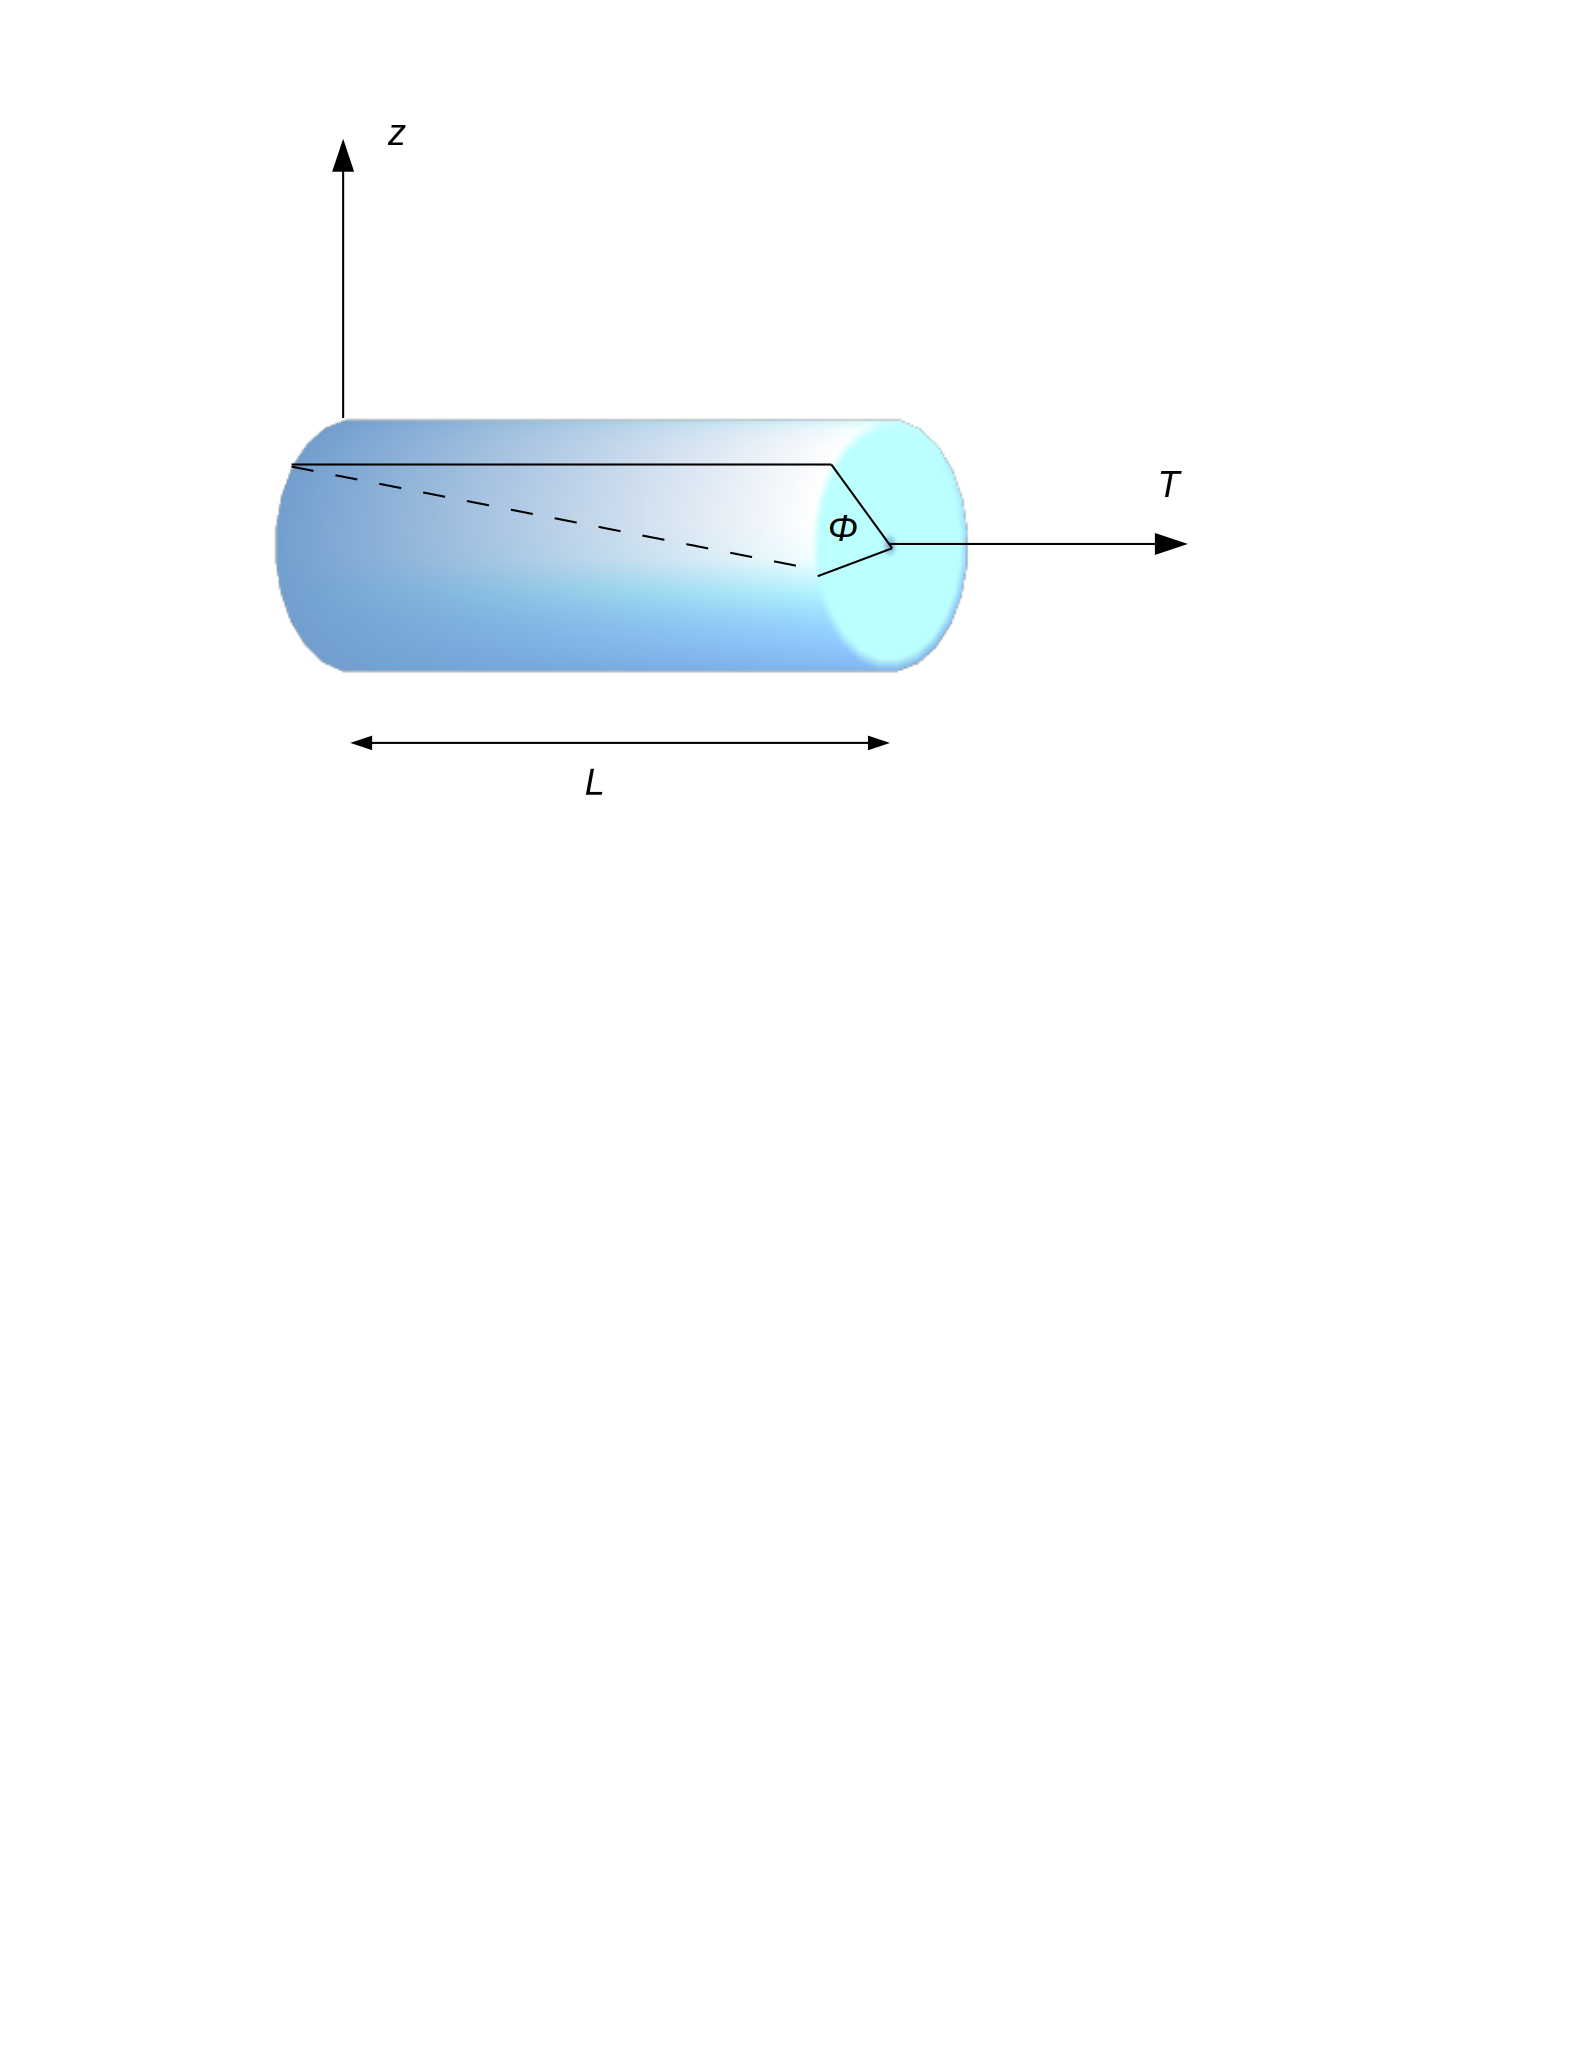
\includegraphics[scale=0.8]{pictures/Static-body-load-analysis/3d-torsion}
  \caption{A circular bar under torsion. The figure shows the torque and deformation on the cross section.}
  \label{fig: 3d torsional deformation}
\end{figure}

Consider a circular bar under torsion in \cref{fig: 3d torsional deformation}. Under the action of torque $T$, if the left-hand end is fixed, the right-hand end will rotate through a small angle $\phi$, known as the angle of twist. The angle of twist changes along the axis of the bar, and at intermediate cross sections it will have a value $\phi(x)$, which we can prove varies linearly between the ends.

The shear strain in an element of length $dx$ is simply the change in the orientation of the originally straight longitudinal line. The change in the orientation can be defined by the angle of change along the length, which is

\begin{equation} \label{eqn: strain and angle of twist}
  \gamma _{\max } = \frac{rd\phi }{dx} = r\theta  = \frac{r\phi }{L}
\end{equation}

where $\theta$ is defined as the angle of twist per unit length, or rate of twist, and $r$ is the radius of the cross-section. Due to symmetry and our assumption that the cross section remains unchanged during the rotation, the radius of the cross section remains undistorted during this time as well, and therefore the shear strain within the interior of the bar radius away from the center is

\begin{equation} \label{eqn: strain and radius}
  \gamma  = \rho \theta  = \frac{\rho }{r}\gamma _{\max }
\end{equation}

Since the bar is in pure shear, we can apply Hooke’s law in shear to analyze the state of stress of the bar in torsion. We have

$$\tau  = G\gamma $$

in which $G$ is the shear modulus of elasticity. We can combine this equation with \cref{eqn: strain and angle of twist} and \cref{eqn: strain and radius} to get

\begin{equation}
  \begin{gathered}
    \tau _{\max } = Gr\theta  \hfill \\
    \tau (\rho ) = G\rho \theta  = \dfrac{\rho }{r}\tau _{\max } \hfill \\ 
  \end{gathered}
\end{equation}

in which $\tau_{max}$ is the shear stress at the outer surface of the bar and $\tau$ is the shear stress at the interior point of radius $\rho$ from the center of the bar.

Now that we have figured out the stress and strain state in a circular bar under torsion, we will now go on to determine the relationship between the external load in the case of torsion, the twisting moment or torque T and the shear stress.

First we consider a small element of area $dA$ located at a radial distance $\rho$ from the center of the bar. The shear force acting on the surface would be $\tau dA$ where $\tau$ is the shear stress at radius $\rho$. The moment from the shear force is simply the force times the distance from the center, $\tau \rho dA$. We can express this small moment as

\[dM = \tau \rho dA = \frac{\tau _{\max }}{r}\rho ^2dA\]

The resultant moment is simply the sum of these small moments across the cross-sectional area

\begin{figure}[h]
  \centering
  \begin{tikzpicture}[>=latex]
    \node[draw, left color=lightblue, right color=lightblue, middle color=lightblue!40, cylinder, rotate=90, minimum width=7cm, minimum height=3cm, inner sep=40](A){};
    \draw[->>, line width=3pt] (A.top) ++ (0,-1.4) node(B){} --++ (90:2cm) node[right]{$dT = \rho \tau dA$};
    \draw[->] (B.center) --++ (-30:1.2) node(C){} node[midway, above right]{$\rho$} node[below left, yshift=-0.2cm]{$dA$};
    \node at (C) [anchor=west, draw, trapezium, trapezium left angle=60, trapezium right angle=-60, fill=LightGrey, minimum width=5mm, minimum height=5mm, rotate=-30](D){};
    \draw[-left to, thick] (D.center) ++ (-150:0.2) --++(30:0.4) node[below]{$\tau$};
    \draw[->] (D.north) -- ++ (30:0.5) node[above right]{$dF=\tau dA$};
  \end{tikzpicture}
  \caption{Torsion formula derivation.}
\end{figure}

\[T = \int_A {dT}  = \frac{\tau _{\max }}{r}\int_A \rho ^2dA  = \frac{\tau _{\max }}{r}J\]

in which $J$ is the polar moment of inertia of the circular cross section. By rearranging this equation, we obtain the maximum shear stress as a function of applied torque:

\begin{equation}
  \tau _{\max } = \frac{Tr}{J}
\end{equation}

This equation is called the torsion formula. Similar to shear strain, the shear stress at a distance $\rho$ from the center of the bar is

\begin{equation}
  \tau  = \frac{\rho }{r}\tau _{\max } = \frac{T\rho }{J}
\end{equation}

Finally, we can also relate the angle of twist of a linearly elastic bar to the applied torque T by combining Hooke’s law in shear and the torsion formula, for which we get

\[\begin{gathered}
    \tau _{\max } = Gr\theta \\
    \tau _{\max } = \frac{Tr}{J} \hfill \\
    \theta  = \frac{T}{GJ} \hfill \\ 
  \end{gathered} \]

This shows that the rate of twist is directly proportional to the torque $T$ and inversely proportional to the product $GJ$. The total angle of twist for the bar in pure torsion is

\begin{equation}
  \phi  = \theta L = \frac{TL}{GJ} = \frac{T}{k_T}
\end{equation}

where $k_T = GJ/L$ is called the torsional stiffness of the bar.

\begin{example} Statically indeterminate torsional analysis in a cylindrical shaft
  
  A circular bar is supported at both ends by ball bearing hubs, allowing them to rotate freely. Three torques are applied along the length of the bar, their magnitudes, directions, and locations are shown in the figure. The bar has diameter of 3 cm, the material it is made of has $G$ = 80 GPa. Find the maximum shear stress in each segment and angle of twist between point B and D.

  \begin{figure}[H]
    \centering
    \begin{tikzpicture}
      \node[fill=white, minimum height=4cm, minimum width=14cm]{};
      \node[draw, cylinder, top color=LightSkyBlue, bottom color=LightSkyBlue, middle color=LightSkyBlue!50, minimum height=11cm, minimum width=1cm, inner sep=2mm](bar){};
      \draw [->>, ultra thick] (bar.west) --++ (180:1) node[above]{275 N-m};
      \draw [->>, ultra thick] (bar.east) ++ (180:0.2) --++ (180:1) node[above]{175 N-m};
      \draw [->>, ultra thick] (bar.east) ++ (180:5.2) node(A){} --++ (0:1) node[above]{450 N-m};
      \draw [|<->|] (A) ++ (-90:1) --++ (180:5.7) node[midway, fill=white]{0.5 m};
      \draw [|<->|] (A) ++ (-90:1) --++ (0:5) node[midway, fill=white]{0.4 m};
    \end{tikzpicture}
    % 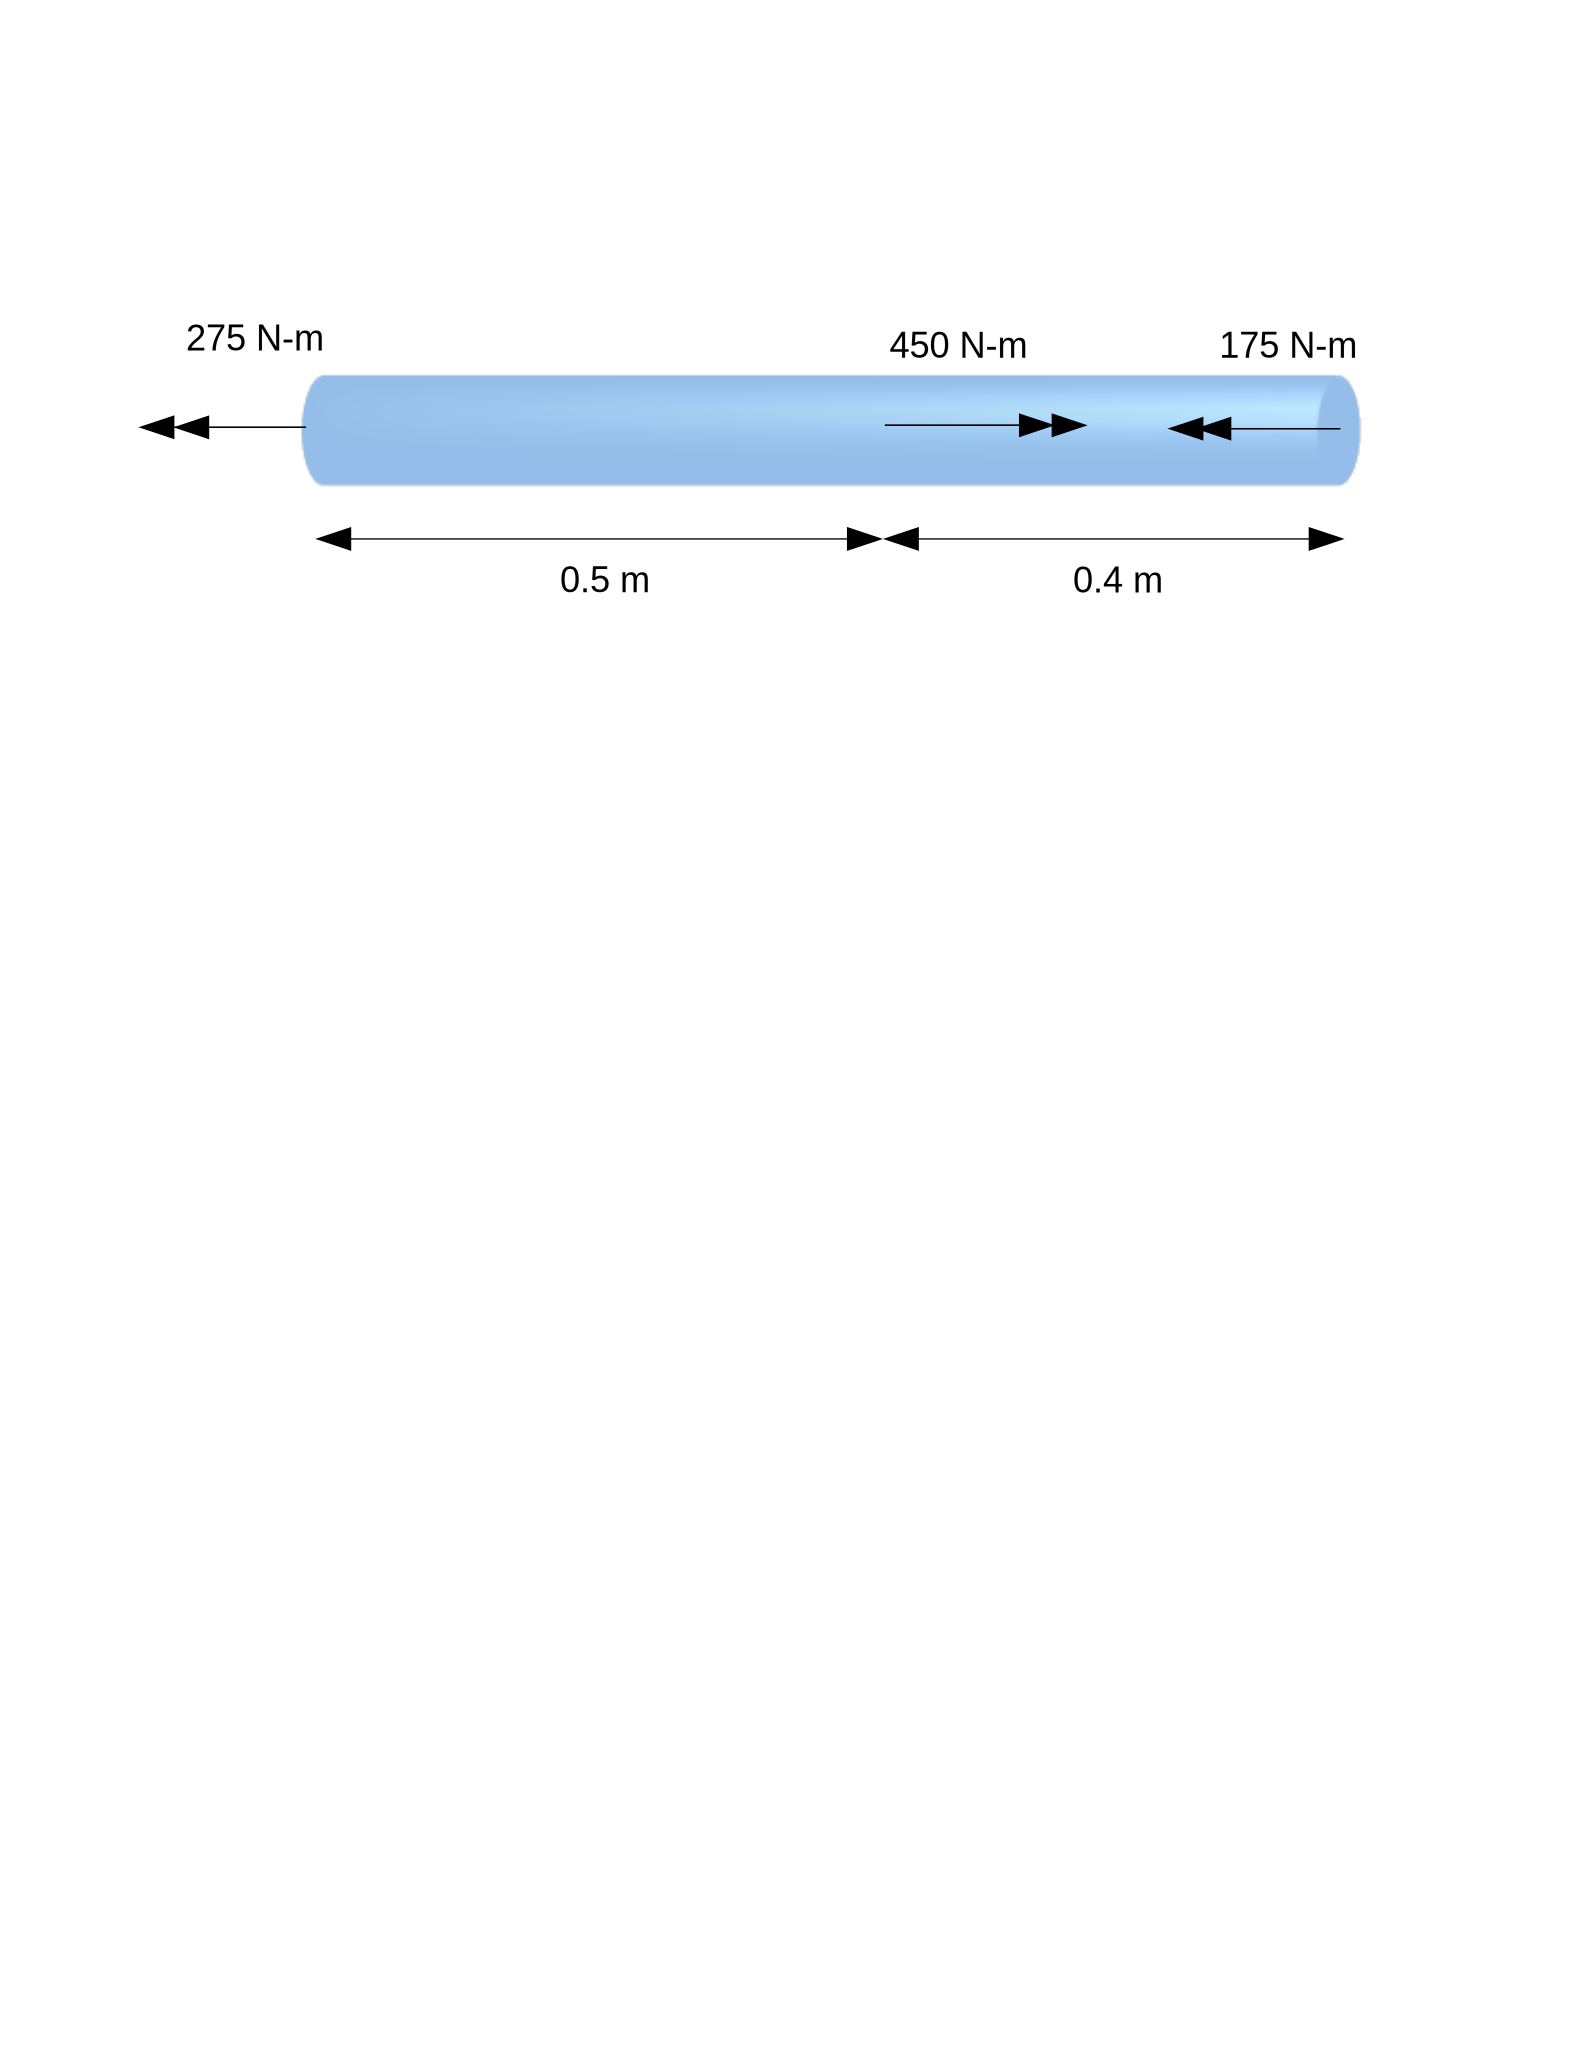
\includegraphics[scale=0.8]{pictures/Static-body-load-analysis/torsion-problem}
  \end{figure}
\end{example}
  
\begin{solution}
First, we need to find the torque in each segment. We can use equation of equilibrium to calculate just that.
Using the method of section, within segment BC,

$$T =  - T_1 =  - 275\text{ Nm}$$

Within segment CD,

\[T =  - T_3 = 175\text{ Nm}\]

The maximum shear stress in each segment is at the outer diameter. We have

\[\begin{gathered}
  \tau _{\max } = \frac{Tr}{J} = \frac{2T}{\pi r^3} \hfill \\
  (\tau _{\max })_{BC} = \frac{2(275\text{ Nm})}{\pi (1.5 \times 10^{ - 2}\text{ m})^3} = 51.9\text{ MPa} \hfill \\
  (\tau _{\max })_{CD} = \frac{2(175\text{ Nm})}{\pi (1.5 \times 10^{ - 2}\text{ m})^3} = 33\text{ MPa} \hfill \\ 
\end{gathered} \]

Angle of twist between B and D is the sum of the angles of twist in BC and CD.

\[\begin{gathered}
  \phi_{BD} = \phi _{BC} + \phi _{CD} \hfill \\
  J = \frac{\pi r^4}{2} = \frac{\pi (1.5 \times 10^{ - 2} \text{ m})^4}{2} =
  7.95 \times 10^{ - 8} \text{ m}^4 \hfill \\
  \phi_{BC} = \frac{T_{BC}L_1}{GJ} = \frac{( - 275\text{ Nm})(0.5\text{ m})}{(80\text{ GPa})(7.95 \times 10^{-8}\text{ m}^4)} =  - 0.0216\text{ rad} \hfill \\
  \phi_{CD} = \frac{T_{CD}L_2}{GJ} = \frac{(175\text{ Nm})(0.4\text{ m})}{(80\text{ GPa})(7.95 \times 10^{-8}\text{ m}^4)} = 0.0110\text{ rad} \hfill \\
  \phi_{BD} =  - 0.0216 + 0.0110 =  - 0.0106\text{ rad} \hfill \\ 
\end{gathered} \]

Therefore, the bar twisted in the same direction as $T_2$ by 0.0106 rad.
\end{solution}

\subsection{Nonuniform Torsion}

In the case of nonuniform torsion, we have loosened the restrictions previously and implicitly imposed on the previous section which are that the bar must be of constant cross section and that the torque throughout the length of the bar must be constant. In this case, we will use the method of sections and apply the principles already explained in the previous section to analyze nonuniform torsion.

To illustrate the procedure, we will divide nonuniform torsion problems into 3 cases.
\begin{enumerate}
\item Bar consisting of constant cross section segments with constant torque throughout each segment. For example, as the figure shows, the bar is made up of three constant cross segments. and throughout each cross section there is a constant torque.
  
  To analyze this problem, we simply use the method of section to determine the torque throughout each cross section. Once the internal torques is determined, we can apply the equations to find the shear stress or the angle o twist in each segment. The total angle of twist of the bar is simply the sum of the angles of twist for all segments. So we have that

    \begin{figure}[h]
    \centering
    \begin{tikzpicture}
      % members
      \draw[fill=LightBlue] (0,0) rectangle (3,1) ;
      \draw[fill=LightBlue] (3,-0.5) rectangle (5,1.5);
      \draw[fill=LightBlue] (5,-0.25) rectangle (7.5,1.25);
      \draw[->>,ultra thick] (7.5,0.5) -- (8.5,0.5) node[right]{$T$};
      \draw[->>,ultra thick] (0,0.5)  -- (-1,0.5) node[left]{$T$};
      % lengths
      \draw[|<->|] (0,-1.5) -- (1.5,-1.5) node[above]{$L_1$} -- (3,-1.5);
      \draw[|<->|] (3,-1.5)-- (4,-1.5) node[above]{$L_2$} -- (5,-1.5);
      \draw[|<->|] (5,-1.5)-- (6.25,-1.5) node[above]{$L_3$} -- (7.5,-1.5);
      % areas
      \draw[<->] (1,0) -- (1, 0.5) node[right]{$A_1$} -- (1,1);
      \draw[<->] (4,-0.5) -- (4, 0.5) node[right]{$A_2$} -- (4,1.5);
      \draw[<->] (6,-0.25) -- (6, 0.5) node[right]{$A_3$} -- (6,1.25);
    \end{tikzpicture}
    \caption{Torque-loaded member with segments of constant cross sections.}
  \end{figure}
  
  \begin{equation}
    \begin{gathered}
      \phi  = \phi_1 + \phi_2 + \phi_3 +  \ldots  \hfill \\
      \phi  = \sum\limits_{i = 1}^n \phi_i = \sum\limits_{i = 1}^n \dfrac{T_iL_i}{G_iJ_i}  \hfill \\ 
    \end{gathered}
  \end{equation}
  
  where $i$ indicates the numbering index for various segments.
  
\item Bar with continuously varying cross sections and constant torque. When the torque is constant, the maximum shear stress in a solid bar always occurs at the cross section having the smallest diameter. To find the angle of twist, we can consider an element of length $dx$ at distance $x$ from one end of the bar. The differential angle of twist $\phi$ is

  \begin{figure}[h]
    \centering
    \begin{tikzpicture}
      \draw[top color=LightSkyBlue, bottom color=LightSkyBlue, middle color=LightSkyBlue!20] (0,-0.5) -- (5,0) -- (5,1) -- (0,1.5) -- (0,-0.5);
      \draw[->>,ultra thick] (5,0.5) -- (6,0.5) node[right]{$T$};
      \draw[->>,ultra thick] (0,0.5)  -- (-1,0.5) node[left]{$T$};
      \draw[<->] (0,-1.5) -- (2.5,-1.5) node[above]{$L$} -- (5,-1.5);
      \draw[<->] (0,-1) -- (0.5,-1) node[above]{$x$} -- (1,-1);
      \draw[<->] (1,-0.4) -- (1, 0.5) node[right]{$J(x)$} -- (1,1.4);
    \end{tikzpicture}
    \caption{Deformation of a torque-loaded variable cross-sectioned member.}
  \end{figure}
  
  \[d\phi  = \frac{Tdx}{GJ(x)}\]

  in which $J(x)$ is the polar moment of inertia of cross section at distance x from the end. The angle of twist of the entire bar is the sum of the differential angles of twist:

  \begin{equation}
    \phi  = \int_0^L \frac{Tdx}{GJ(x)}
  \end{equation}

  If the expression for the polar moment of inertia is not too complex, the integral can be evaluated analytically; in other cases, however, it must be evaluated numerically.

\item Bar with continuously varying cross sections and continuously varying torque. The bar can be subjected to a distributed torque that varies along the length of an also varying cross section bar. We can use the method of sections to find the torque along the length of the bar. We also need to find the polar moment of inertia along the length of the bar. Once we know both quantities, we can use the torsion formula to determine the shear stress. The angle of twist can also be found in the same manner as case 2 except now the torque is also varying. So the equation for the total angle of twist becomes
  
  \begin{figure}[h]
    \centering
    \begin{tikzpicture}
      \draw[top color=LightSkyBlue, bottom color=LightSkyBlue, middle color=LightSkyBlue!20] (0,-0.5) -- (5,0) -- (5,1) -- (0,1.5) -- (0,-0.5);
      \draw[->>,ultra thick] (1,0.5) -- (2,0.5) node[right]{$T(x)$};
      \draw[<->] (0,-1.5) -- (2.5,-1.5) node[above]{$L$} -- (5,-1.5);
      \draw[<->] (0,-1) -- (0.5,-1) node[above]{$x$} -- (1,-1);
      \draw[<->] (1,-0.4) -- (1, 0.5) node[left]{$J(x)$} -- (1,1.4);
    \end{tikzpicture}
    \caption{Deformation of a torque-loaded variablecross-sectioned member.}
  \end{figure}
  
  \begin{equation}
    \phi  = \int_0^L \frac{T(x)dx}{GJ(x)}
  \end{equation}

  This integral usually must be evaluated numerically.
\end{enumerate}

\section{Bending} \label{section: bending}

When external load is applied perpendicular to the axis of the length of the beam, it will create a shear force and/or bending moment inside the beam. The deformation from this type of load is called deflection. In this chapter, we will analyze the relationship between the external load, the shear force, the bending moment, and the deflection of the beam.

\subsection{Pure Bending}

First we will consider the simplest case of bending where the cross section of the beam in consideration has at least one axis of symmetry, and that the applied load is in the same plane as the axis of symmetry. This will cause bending in the plane of symmetry, resulting in symmetric beam bending.

\subsection{Longitudinal strains in beams}

The longitudinal strain in a beam can be found by analyzing the curvature of the beam and the associated deformations. For this purpose, let us consider a portion of a beam in pure bending subjected to positive bending moment $M$. Under the action of the bending moments, the beam deflects in the $xy$ plane and its longitudinal axis is bent into a circular curve. Cross sections of the beam are assumed to remain plane and normal to the longitudinal axis.

\begin{figure}[h]
  \centering
  \begin{tikzpicture}
    \node at (0,0) (O){} node[right]{$O$};
    \draw [dashed] (O.center) -- ++(-120:5) node(A){};
    \draw [line width=40pt, LightSkyBlue] (A.center) arc (-120:-60:5) node(B){};
    \draw [dash dot] (A.center) arc (-120:-60:5) node[near start](y){};
    \draw [->] (y.center) --++ (75:0.3) node(C){} node[midway, left]{$y$};
    \draw [<-] (C.center) -- (O.center) node[midway, left]{$\rho - y$};
    \draw [dash dot] (A.center) ++ (60:0.3) arc (-120:-60:4.7) node(D){};
    \draw [->] (D.center) --++ (45:0.5) node[right]{$(\rho - y)d\theta$};
    \draw [->] (B.center) --++ (0:0.5) node[right]{$\rho d\theta$};
    \draw [dashed] (B.center) -- (O.center);
    % \draw [<->, black!50] (O.center) ++ (90:1) --++ (-90:8);
    \draw [<->, black!50] (O.center) ++ (-90:5) ++ (180:4) --++ (0:8) node[below, black]{$x$};
    \draw [->] (O.center) --++ (-70:5) node[midway, left]{$\rho$};
    \draw (O.center) ++ (-60:1) arc (-60:-120:1) node[midway, above]{$d\theta$};
    %\draw [dashed] (O.center) --++ (-100:5) node[midway, left, yshift=-3mm]{};
    %\draw [dashed] (O.center) --++ (-110:5);
  \end{tikzpicture}
 % 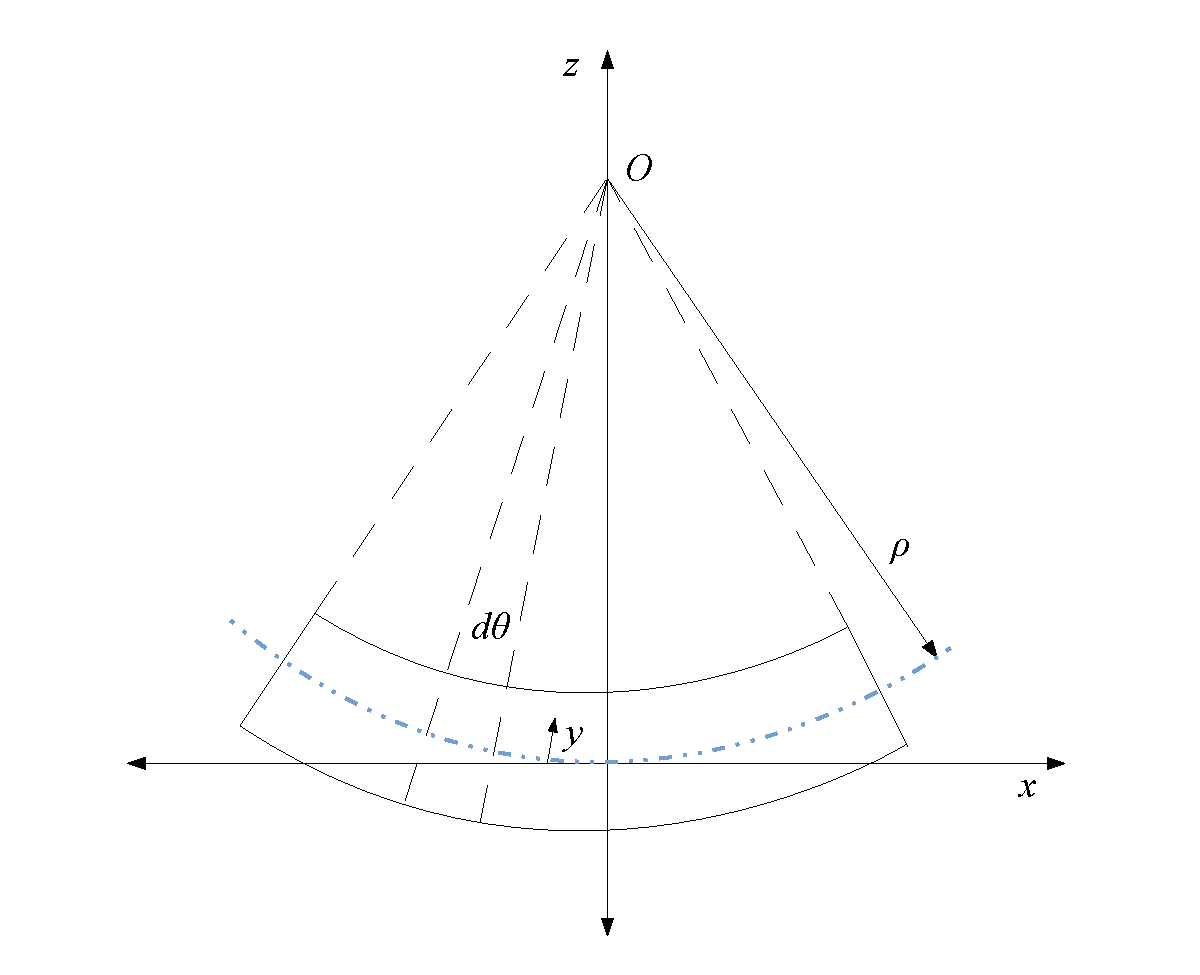
\includegraphics[scale=0.6]{pictures/Static-body-load-analysis/pure-bending}
  \caption{Deformation in pure beam bending.}
  \label{fig: pure bending}
\end{figure}


Because of the bending deformations, cross sections rotate with respect to each other about axes perpendicular to $xy$ plane. As shown in \cref{fig: pure bending}, longitudinal lines of the convex part of the beam are elongated, while those on the concave side are shortened. Therefore, the lower part of the beam is in tension while the upper part is in compression. Somewhere between the top and bottom surface there is a surface where its longitudinal lines do not change in length. This surface is called the \emph{neutral surface}. Its intersection with any cross-sectional plane is called the neutral axis of the cross section.

The planes containing cross sections intersect in a line through the center of curvature. The angle between the two planes is denoted $d\theta$ and the distance to the neutral surface is the radius of curvature $\rho$. The initial distance between the two planes is unchanged at the neutral surface and thus $\rho d \theta = dx$. However, all other lines not on the internal surface either lengthen or shorten, creating normal strains.

To evaluate the normal strains, consider a longitudinal line located at a distance y away from the neutral surface in an initially straight beam. Once the beam deflects, the neutral surface moves with the beam, but the x axis remains fixed and therefore the longitudinal line is still located at the same distance $y$ away. The new length of this longitudinal line becomes

\[(\rho  - y)d\theta  = dx - \dfrac{y}{\rho }dx\]

Therefore, the corresponding normal strain of this longitudinal line is simply the change in length divided by the original length, which is

\begin{equation}
  \varepsilon _x = \frac{dx - \dfrac{y}{\rho }dx - dx}{dx} =  - \dfrac{y}{\rho } =  - \kappa y
\end{equation}

where $\kappa$ is the curvature.

Note the negative sign in the equation; when the point of interest is above the neutral surface, the part is in compression, and vice versa.

The next step in our analysis is to find the stresses from the strains, which derive from Hooke’s law for linearly elastic materials.

\subsection{Normal stresses in beams}

Since we have established the relationship between the distance of the point of interest from the neutral surface and the normal strain in bending beam, we can now apply Hooke’s law for linearly elastic material to derive the stress in the beam.

\begin{figure}[h]
  \centering
  \begin{tikzpicture}
    \draw [fill=SkyBlue] (0,0) arc [radius=9, start angle=120, end angle=90] --
    ++(90:2) arc [radius=11, start angle=90, end angle=120] -- (0,0);
    \draw[->, thick] (-1.5,2) arc (135:250:1.5cm);
    \draw[dashed, thin] (-0.5,0.866) arc (120:90:10cm);
    \foreach \x in {0,...,10}
    \draw[->] (4.5,3.2 - 0.2*\x) -- ++(0: 1-0.2*\x);
    \draw[->, thick] (6, 3.5) arc (60:-60:1.5);
    \draw (-2.5,1) node{$M$};
    \draw (7, 2.5) node{$M$};
    \draw (5.4,3.1) node[right]{$+\sigma$};
    \draw (3.6,1.4) node[left]{$-\sigma$};
  \end{tikzpicture}
  \caption{Bending stress in uniform bending.}
\end{figure}

\begin{equation} \label{eqn: stress-strain bending}
  \sigma_x = E\varepsilon_x =  - E\frac{y}{\rho } =  - E\kappa y
\end{equation}

This equation shows that the normal stresses, just like normal strains, vary linearly with the distance $y$ from the neutral surface. For example, when the bending moment $M$ is positive and the beam bends with positive curvature, the stresses are negative (compression) above the neutral surface and positive (tension) below it.

However, in order for \cref{eqn: stress-strain bending} to be useful, we must first determine the location of the neutral axis on the cross section so that we may find the distance of the point of interest from it.

The location of the neutral axis can be determined by employing a static equilibrium equation. We know that the resultant force on any cross section of the beam is zero. We may then apply \cref{eqn: stress-strain bending} using this fact, thus we have

\[\int_A\sigma_x dA  =  - \int_A E\kappa ydA  = 0\]

Since the curvature and the modulus of elasticity are constants at any cross section of the beam, we have

\begin{equation}
  \int_A ydA = 0
\end{equation}

This equation states that the first moment of the area of the cross section, evaluated with respect to the neutral axis, is zero. In other words, the neutral axis must pass through the centroid of the cross section.

\subsection{Moment-curvature formula}

We also know that the resultant moment of the normal stresses acting over the
cross section must be equal to the bending moment at that cross section. Let us
first consider the element of force $\sigma xdA$ acting on the element of area
$dA$ is in the positive direction when $\sigma_x$ is positive. If the element $dA$ is located above the neutral axis, a positive stress would produce an
element of moment in $\sigma_xydA$ the negative direction since it tends to bend
the beam downward. Therefore, we have

\begin{figure}[h]
  \centering
  \begin{tikzpicture}
    \draw [fill=SkyBlue] (0,0) arc [radius=9, start angle=120, end angle=90] --
    ++(90:2) arc [radius=11, start angle=90, end angle=120] -- (0,0);
    \draw[dashed, thin] (-0.5,0.866) arc (120:90:10cm);
    \foreach \x in {1}
    \draw[->] (4.5,3.2 - 0.2*\x) -- ++(0: 1-0.2*\x) node(B){} node[above]{$\sigma dA$};
    \draw[->, thick] (B.east) ++ (0:0.5) arc (75:-75:0.7) node[midway, right]{$dM = \sigma y dA$};
    \draw[|<->|] (4.3,2.2) -- (4.3, 3.0) node[below left]{$y$};
  \end{tikzpicture}
  \caption{Infinitessimal bending moment $dM$ generated from force $\sigma dA$ with a distance $y$ from the neutral axis.}
\end{figure}

\[dM =  - \sigma _xydA\]

The sum of all the elemental moments of the entire cross section is simply the bending moment:

\[M =  - \int_A \sigma_xydA \]

By substituting $\sigma_x = -E\kappa y$, we have

\[M =  - \int_A \kappa Ey^2dA  =  - \kappa E\int_A y^2dA \]

which we can define as

\[\begin{gathered}
  M = \kappa EI \hfill \\
  I = \int_A y^2dA  \hfill \\ 
\end{gathered} \]

where $I$ is called the moment of inertia. We can now rearrange equation 3.43 in terms of the bending moment as

\begin{equation} \label{eqn: moment-curvature}
  \kappa  = \frac{1}{\rho } = \frac{M}{EI}
\end{equation}

This equation is known as the moment-curvature equation, showing that the curvature of the bending beam is directly proportional to the bending moment and inversely proportional to the quantity $EI$, which is called the \emph{flexural rigidity} of the beam.

\subsection{Elastic Flexure Formula}

Now that we have located the neutral axis and derived the moment-curvature relationship, we can determine the stress inside the beam from the bending moment. Substituting \cref{eqn: moment-curvature} into \cref{eqn: stress-strain bending}, we have

\begin{equation} \label{eqn: flexure formula}
  \sigma_x =  - \frac{My}{I}
\end{equation}

This equation is called the flexure formula, shows that the stresses are directly proportional to the bending moment $M$ and inversely proportional to the moment of inertial $I$. The stresses also vary linearly with the distance $y$ from the neutral axis.

\subsection{Maximum stress at a cross section}

From \cref{eqn: flexure formula}, we know that the maximum tensile stress and compressive stress on a given cross section occurs at points located the furthest away from the neutral axis. Assume the distance from the neutral axis to the extreme elements above and below to be $c_1$ and $c_2$ respectively, then the corresponding maximum normal stresses from the flexure formula are

\begin{equation} \label{eqn: section modulus}
  \begin{gathered}
    \sigma _1 =  - \frac{Mc_1}{I} =  - \frac{M}{S_1} \hfill \\
    \sigma _2 =  - \frac{Mc_2}{I} =  - \frac{M}{S_2} \hfill \\ 
  \end{gathered}
\end{equation}

in which

\[\begin{gathered}
  S_1 = \frac{I}{c_1} \hfill \\
  S_2 = \frac{I}{c_2} \hfill \\ 
\end{gathered} \]

The quantities $S_1$ and $S_2$ are known as the section moduli of the cross section.

\subsection{Shear stresses in beams}

When the beam is in pure bending, there are only bending moments and normal stresses in the cross sections. However, most beams are subjected to loads that produce both bending moments and shear forces, resulting in nonuniform bending. In this case, both normal and shear stresses are developed in the beam.

To derive the formula for the shear stresses in a rectangular beam, we instead evaluate the vertical horizontal shear stresses acting between layers of the beam due to convenience, since both have the same magnitudes.

Let us consider a beam in nonuniform bending. Take an element with two adjacent cross sections $mn$ and $m_1n_1$ with distance $dx$ apart. On the left hand face, the bending moment $M$ and shear force $V$ is applied. Since the beam is in nonuniform bending, the bending moment and shear force may change along the length of the beam, and the corresponding quantities on the right hand face are $M + dM$ and $V + dV$.

\begin{figure}[h]
  \centering
  \begin{tikzpicture}[>=latex]
    \node at (0,0) [draw, cylinder, fill=lightblue, minimum height=5cm, minimum width=3cm, inner sep=6pt](A){};
    \draw [dashed] (A.north) ++ (180:0.3) node[above]{$m$} --++ (-90:3) node[midway](p){} node[midway, left]{$p$} node[below](B){$n$};
    \draw [dashed] (A.north) ++ (0:0.3) node[above]{$m_1$} --++ (-90:3) node[midway](p1){} node[midway, right]{$p_1$} node[below](C){$n_1$};
    \draw [dashed] (p.center) -- (p1.center);
    \draw [->] (B) ++ (135:1) arc (240:120:1) node[near start, below left]{$M$};
    \draw [->] (C) ++ (45:1) arc (-60:60:1) node[near start, below right]{$M+dM$};

    % small element
    \node at (6,0) [anchor=south west, draw, rectangle, fill=lightblue, minimum height=1.5cm, minimum width=0.6cm](E){};
    \foreach \x in {0,...,4}
    \draw [<-] (E.north west) ++ (-90:0.375*\x) --++ (180:1-0.24*\x);
    \node at (E.north west) [xshift=-1.2cm, yshift=-0.8cm]{$\sigma_1$};
    \foreach \x in {0,...,4}
    \draw [<-] (E.north east) ++ (-90:0.375*\x) --++ (0:1.2-0.29*\x);
    \node at (E.north east) [xshift=1.2cm, yshift=-0.8cm]{$\sigma_2$};
    \draw [-right to, thick] (E.south west) ++ (-90:0.2) --++ (0:0.6) node[midway, below](F){$\tau$};
    \node at (E.north west) [xshift=-1.9cm, yshift=-0.8cm](left){\Large$\Bigg\{$};
    \node at (left.west) {$F_1$};
    \node at (E.north east) [xshift=1.9cm, yshift=-0.8cm](right){\Large$\Bigg\}$};
    \node at (right.east) {$F_2$};
    \node at (F.south) [rotate=90] {$\Bigg\{$};
    \node at (F.south) [yshift=-0.4cm] {$F_3$};
  \end{tikzpicture}
\end{figure}

On cross section $mn$ and $m_1n_1$, the normal stresses are

\[\begin{gathered}
  \sigma _1 =  - \frac{My}{I} \hfill \\
  \sigma _2 =  - \frac{(M + dM)y}{I} \hfill \\ 
\end{gathered} \]

Next, we separate a small subelement $mm_1pp_1$ by passing a horizontal plane through our initial element. Since the bending moments vary along the axis of the beam, the normal forces acting on the left hand and right hand sides are no longer of the same magnitude. The forces on the left $F_1$ and right side $F_2$ respectively, are

\begin{gather*}
    F_1 = \int \frac{My}{I}dA \hfill \\
    F_2 = \int \frac{(M + dM)y}{I}dA \hfill
\end{gather*}

The rest of the force must be balanced by the shear force $F_3$, which gives us

\[\begin{gathered}
  F_3 = F_2 - F_1 = \int \frac{(M + dM)y}{I}dA  - \int \frac{My}{I}dA  \\ 
   = \int \dfrac{(dM)y}{I}dA \\ 
 \end{gathered} \]

Rearranging this equation, we have

\begin{equation} \label{eqn: shear stress eval}
  F_3 = F_2 - F_1 = \frac{dM}{I}\int y dA
\end{equation}

Assuming the shear stress is evenly distributed across the width b of the beam, making the area the shear force is acting upon is $bdx$, gives us

\[F_3 = \tau bdx\]

Substitute this into \cref{eqn: shear stress eval} and solve for shear stress gives

\[\tau  = \frac{dM}{dx}\left( \frac{1}{Ib} \right) \int ydA \]

We know that the quantity $dM/dx$ is equal to the shear force $V$. The integral is evaluated over the part of the cross section that we have chosen earlier. It represent the first moment of the partial cross section with respect to the neutral axis. If we denote the first moment by $Q$, we have

\begin{equation}
  \tau  = \frac{VQ}{Ib}
\end{equation}

This equation, known as the \emph{shear formula}, can be used to determine shear stress at any point in the cross section of a rectangular beam. Note that for a specific cross section, the shear force $V$, the moment of inertia $I$, and the cross-sectional width $b$ are constant; only the first moment $Q$ changes with the distance $y$ from the neutral axis.

\subsection{Beam deflection} \label{subsection: beam deflection}

In certain engineering applications, it is more important to understand the deformation, or deflection, of a beam due to bending moment or shear force itself than the stresses generated from it. In previous sections we have developed a method to determine the normal and shear stresses in bending beams. However, we have not yet developed a method to determine the deflections themselves. In this section, we will determine the equation of the deflection curve and also find deflections at specific points along the axis of the beam.

Deflections are sometimes calculated in order to verify that they are within tolerable limits. For examples, specifications for the design of buildings usually place upper limits on the deflections, preventing cracks in ceilings and walls from large deformation. In the design of machines and aircraft, specifications may limit deflections in order to prevent undesirable vibrations.

There are mainly two methods widely used in calculating the deflection of the beam. The first method is based on using the relationship between the bending moment and the curvature in the beam. As we have discussed, the curvature of the beam is simply the second derivative of the deflection of the beam along its length and, therefore, to obtain the deflection curve, on must integrate the curvature of the beam. We will call this the \emph{direct integration approach}. The second method is based on the relationship between the strain energy in the bending beam and applied load. Therefore, this method is called the \emph{energy approach}.

\subsubsection{Direct Integration Approach}

For the purpose of discussion, we will assume that the beam has its original orientation along the x axis. The deflection, denoted with v, is the lateral deformation of the beam along the y axis at any position x along the length of the beam.

When the beam is bent, there is not only a deflection at each point along the axis but also a rotation. The angle of rotation $\theta$ of the axis of the beam is the angle between the x axis and the tangent to the deflection curve. If $\rho$ is the radius of curvature and $s$ is the length of the curve, we see

\begin{figure}[h]
  \centering
  \begin{tikzpicture}
    % entire cantilever
    \draw[pattern=north west lines] (0,-0.5) rectangle (1,2.5);
    \draw [lightblue, line width=10pt] (1,1)  node(A){} arc (90:70:20)  node[near start](B){} node[near end](C){} node(D){};
    \draw [dashed] (1,1) arc (90:70:20);
    \draw [|<->|] (A.center) ++ (90:0.5) arc (90:85:20.5) node[midway, above]{$ds$};
    \draw[->] (A.north) ++ (90:1) --++ (0:1) node[above left]{$x$};
    %\draw [->, ultra thick] (D.center) --++ (-90:1) node[below]{$P$};
    \draw [dashed] (A.center) --++ (-90:5) node(O){} node[above right, yshift=1cm, xshift=-0.1cm]{$d \theta$} -- (B.center) node[midway, right]{$\rho$};

    \draw (C.center) --++ (-90:0.53) node[midway, left]{$dv$} -- (D.center) node[midway, below]{$dx$};
    \draw [<-] (D.west) ++ (170:0.5) --++ (30:1.5) node[right]{$\theta$};
  \end{tikzpicture}
  \caption{Relationship in bending beam among radius of curvature, curve length, angle of rotation, deflection, and length.}
\end{figure}

\[ \rho d\theta  = ds \]

Therefore, the curvature $\kappa$ is given by the equation

\begin{equation} \label{eqn: deflection curve}
  \kappa  = \frac{1}{\rho } = \frac{d\theta }{ds}
\end{equation}

The slope of the deflection curve is the first derivative $dv/dx$ of the deflection curve. Since both $dv$ and $dx$ are very small, the slope $dv/dx$ is simply the tangent of the angle of rotation. Thus

\begin{equation} \label{eqn: tan approx}
  \frac{dv}{dx} = \tan \theta
\end{equation}

In similar manner, we also obtain the following relationships:

\[\cos \theta  = \frac{dx}{ds} \text{ and } \sin \theta  = \frac{dv}{ds}\]

Since these derivations are based only upon geometric considerations, they are valid for beams of any material. Furthermore, there are no restrictions on the magnitudes of the slopes and deflections.

When we assume that the beam undergo only very small deflections and angles of rotation, in this case, it is acceptable to assume that the curvature of the beam is very small. For very small angle, $\cos\theta \approx 1$, giving

\[ds \approx dx\]

And so \cref{eqn: deflection curve} becomes

\begin{equation} \label{eqn: deflection curve 2}
  \kappa  = \frac{1}{\rho } = \frac{d\theta }{dx}
\end{equation}

Also, when the angle is small $\tan\theta \approx \theta$ so we can simplify \cref{eqn: tan approx} to

\[\theta  = \frac{dv}{dx}\]

Substituting this into \cref{eqn: deflection curve 2} and we have

\[\kappa  = \frac{1}{\rho } = \frac{d^2v}{dx^2}\]

This equation is valid for a beam of any material provided the rotations are small.

If we assume that the material of a beam is linearly elastic and follows Hooke’s law, and that the curvature of the beam follows \cref{eqn: moment-curvature}, then we can derive the \emph{differential equation of the deflection curve} as

\begin{equation} \label{eqn: diff equation of deflection}
  \frac{d^2v}{dx^2} = \frac{M}{EI}
\end{equation}

This equation can be integrated to find the deflection, provided the bending moment $M$ and flexural rigidity $EI$ are known as a function of $x$.

Other equations can be obtained by replacing the bending moment $M$ with the shear force $V$ and the intensity of the distributed load $q$. We know that

\begin{equation} \label{eqn: shear force and load intensity}
  \frac{dM}{dx} = V \hspace{1cm} \frac{dV}{dx} =  - q
\end{equation}

In the case of a nonprismatic beam, the flexural rigidity $EI$ is varying along the length of the beam. We write \cref{eqn: diff equation of deflection} in the form

\[EI\frac{d^2v}{dx^2} = M\]

Differentiating both sides of this equation and substitute values from \cref{eqn: shear force and load intensity} gives

\begin{equation}
  \begin{gathered}
    \frac{d}{dx}\left( EI\frac{d^2v}{dx^2} \right) = V \hfill \\
    \frac{d^2}{dx^2}\left( EI\frac{d^2v}{dx^2} \right) = \frac{dV}{dx} =  -q \hfill \\ 
  \end{gathered}
\end{equation}

In the case of a prismatic beam, the differential equation reduces to

\begin{align}
  EI\frac{d^2v}{dx^2} &= M \nonumber \\
  EI\frac{d^3v}{dx^3} &= V \nonumber \\
  EI\frac{d^4v}{dx^4} &=  - q 
\end{align}

Each time we integrate produces one constant of integration. These constants can be solved for by imposing known conditions regarding the slopes and deflections. The conditions fall into one of these three categories: 1) boundary conditions, 2) continuity conditions, and 3) symmetry conditions.

\emph{Boundary conditions} pertain to the deflections and slopes at the supports of the beam. For example, a simple support keeps the deflection at zero, and at a fixed support both the deflection and slope are zero.

\emph{Continuity conditions} occur where the regions of integration meet. Since the beam is not `broken,' its deflection, slope, and curvature must be continuous through out its length. We can then impose these conditions on the points where the bending moment function changes.

\emph{Symmetry conditions} may be available where supports and loading are symmetric. For example, if a simple beam supports a uniform load throughout its length, the beam's deflection must be symmetric. It can then be deduced that the slope of the deflection at the middle must be zero.

\begin{example}
  If we have a prismatic beam fixed on one end and a vertical load $P$ applied on the other end. What is the deflection curve of the beam and what is the maximum deflection if the beam has properties $E$ and $I$ throughout its length?

  \begin{figure}[H]
    \centering
    \begin{tikzpicture}
      \draw[pattern=north west lines] (0,-0.5) rectangle (1,2.5);
      \draw[fill=SkyBlue] (1,0.75) rectangle (7,1.25);
      \draw[<-, ultra thick] (7,1.25) -- ++(90:1) node[above]{$P$};
      \draw[|<->|] (1, 0.25) -- (4,0.25) node[below]{$L$} --  (7, 0.25);
      \draw (4,1.75) node{$EI$};
      \draw[->] (1,1.75) -- (2,1.75) node[above left]{$x$};
    \end{tikzpicture}
  \end{figure}
  
\end{example}
\begin{solution}
First we must determine the bending moments inside the cross section along the length. Using the method of sections, we can determine that

\[M(x) =  - P(L - x)\]	

We can determine the deflection curve by integrating twice on the equation and apply boundary conditions on the fixed end

\[\begin{gathered}
  EI\frac{d^2v}{dx^2} = M(x) =  - P(L - x) \hfill \\
  EI\frac{dv}{dx} = \frac{P}{2}(L - x)^2 + C_1 \hfill \\
  \frac{dv}{dx} = 0\text{ at }x = 0 \hfill \\
  C_1 =  -\frac{PL^2}{2} \hfill \\
  EI\frac{dv}{dx} = \frac{P}{2}(L - x)^2 - \frac{PL^2}{2} \hfill \\
  EIv =  -\frac{P}{6}(L - x)^3 -\frac{PL^2x}{2} + C_2 \hfill \\
  v = 0\text{ at }x = 0 \hfill \\
  C_2 = \frac{PL^3}{6} \hfill \\
  v =  -\frac{P}{6EI}(L - x)^3 -\frac{PL^2x}{2EI} + \frac{PL^3}{6EI} \hfill \\ 
\end{gathered} \]

The maximum deflection, naturally, is at the free end. Its value is

\[v(L) =  - \frac{PL^3}{2EI} + \frac{PL^3}{6EI} =  - \frac{PL^3}{3EI}\]

Note that the negative sign means the deflection is downward.
\end{solution}

\begin{example} A simply supported beam under a midpoint load.

  A prismatic beam with simply supported ends is loaded with a downward force $P$ in the middle. Determine the deflection curve of the beam and its maximum deflection. Assume that the beam has a flexural stiffness of $EI$.

  \begin{figure}[H]
    \centering
    \begin{tikzpicture}
      \node[draw, rectangle, fill=SkyBlue, minimum height=0.4cm, minimum width=7cm](beam){};
      \node at (beam.south west) [anchor=north, draw, regular polygon, regular polygon sides=3, fill=gray, minimum height=0.5cm, inner sep=0]{};
      \node at (beam.south east) [anchor=north, draw, circle, minimum height=0.3cm, fill=gray, minimum width=0.3cm]{};
      \node at (beam.south) [yshift=-0.3cm] {$EI$};
      \draw[<-, ultra thick] (beam.north) -- ++(90:1) node[above]{$P$};
      \draw[|<->|] (beam.south west) ++ (-90:1) --++ (0:7) node[midway, below]{$L$};
      \draw[->] (beam.north west) ++ (90:0.3) --++ (0:1) node[midway, above]{$x$};
    \end{tikzpicture}
  \end{figure}
  
\end{example}
\begin{solution}

  We first need to determine the bending moment function of the beam along its length. Employing the method of section and replacing each end support by a support force of $P/2$, we proceed to cut the beam from the left side, for which we have

  \begin{align*}
    M(x) &= P\frac{x}{2}
  \end{align*}

  This function, however, true only up to the length $x = L/2$. Beyond this point, we will have to take into account the bending moment generated by the downward for $P$.

  \begin{align*}
    M(x) &= P\frac{x}{2} - P(x-\frac{L}{2}) \\
         &= \frac{P}{2}(L-x)
  \end{align*}

  In summary, the bending moment function along the length of the beam is

  \begin{equation*}
    M(x) = \left\{
      \begin{array}{l l l}
        P\dfrac{x}{2} & & x \leqslant \dfrac{L}{2} \\[1em]
        \dfrac{P}{2}(L-x) & & x \geqslant \dfrac{L}{2}
      \end{array} \right.
  \end{equation*}

  Notice that by substituting $x = L/2$ in either equation yield the same bending moment. 

  Now, using this expression in the direct integration method. For $x \leqslant L/2$, we have

  \begin{align*}
    EI \frac{d^4v}{dx^4} &= EIv'' = P\frac{x}{2}dx \\
    EIv' &= P (\frac{x^2}{4}) + C_1 \\
  \end{align*}

  We can use a continuous boundary condition at $x = L/2$ to solve for $C_1$ once we have obtained the functional form of the deflection curve for $x \geqslant L/2$. Preferably, we can also solve for $C_1$ by applying symmtetry condition. In other words, we know that the problem is symmetric about the axis $x = L/2$, and thus the slope of the beam in the middle \emph{must} be zero. This way, we do not need to know the functional form of the right half of the deflection curve.

  \begin{align*}
    EIv'(x= \frac{L}{2}) = 0 &= P \left( \frac{L^2}{16} \right) + C_1 \\
    C_1 &= -P \left( \frac{L^2}{16} \right) \\
    EIv' &= P \left( \frac{4x^2 - L^2}{16} \right)
  \end{align*}

  Integrating one more time to obtain the left-half curve.

  \begin{align*}
    EIv &= \frac{P}{16} \left( \frac{4}{3}x^3 - L^2x \right) + C_2
  \end{align*}

  Simple support at $x = 0$ means there is no vertical deflection at the point.

  \begin{align*}
    EIv(x=0) &= 0 = C_2
  \end{align*}

  The left-half deflection curve is

  \begin{equation*}
    v(x) = \frac{P}{16EI} \left( \frac{4}{3}x^3 - L^2x \right)
  \end{equation*}
  
  We can proceed with the right-half in similar fashion.

  \begin{align*}
    EIv'' &= \frac{P}{2}(L - x) \\
    EIv' &= \frac{P}{2}(Lx - \frac{x^2}{2}) + C_3
  \end{align*}

  Solving for zero slope in the middle.

  \begin{align*}
    EIv'(x = \frac{L}{2}) &= 0 = \frac{P}{2} \left( \frac{L^2}{2} - \frac{L^2}{8} \right) + C_3 \\
    C_3 &= -\frac{3PL^2}{16} \\
    EIv' &= \frac{P}{2} \left( Lx - \frac{x^2}{2} - \frac{3L^2}{8} \right)
  \end{align*}

  Integrate one last time to obtain the right-half curve.

  \begin{align*}
    EIv &= \frac{P}{2} \left( \frac{Lx^2}{2} - \frac{x^3}{6} - \frac{3L^2x}{8} \right) + C_4 \\
    v(x &= L) = 0 \\
    0 &= \frac{P}{2} \left( \frac{L^3}{2} - \frac{L^3}{6} - \frac{3L^3}{8} \right) + C_4 \\
    C_4 &= P \frac{L^3}{48} \\
  \end{align*}

  The right-half deflection curve is

  \begin{equation*}
    v(x) = \frac{P}{4EI} \left( Lx^2 - \frac{x^3}{3} - \frac{3L^2x}{4} + \frac{L^3}{12} \right)
  \end{equation*}

  Due to symmetry in this problem, it is relatively simple to tell that the maximum deflection occurs at $x = L/2$. In asymmetric problems, it may be necessary to rely on calculus to determine the location with the maximum deflection.

  Substitute either the left- or right-half deflection curve with $x = L/2$ to obtain the maximum deflection. In this problem, we do the right-half first.

  \begin{align*}
    &v(x = \frac{L}{2}) = \frac{P}{4EI} \left( \frac{L^3}{4} - \frac{L^3}{24} - \frac{3L^3}{8} + \frac{L^3}{12} \right) \\
    &v_{\max} = \frac{-4PL^3}{4(48)EI} = -\frac{PL^3}{48EI}
  \end{align*}

  We can also substitute $x = L/2$ into the left-hand to double-check our answer.

  \begin{align*}
    &v(x = \frac{L}{2}) = \frac{P}{16EI} \left( \frac{4L^3}{24} - \frac{L^3}{2}\right) \\
    &v_{\max} = \frac{P}{16EI} \frac{-L^3}{3} = -\frac{PL^3}{48EI}
  \end{align*}
  
\end{solution}  

\subsubsection{Energy approach (Castigliano’s theorem)} \label{subsub: energy method}

This theorem provides a method for finding the deflections of a structure from its strain energy. The theorem simply states that the derivative of the strain energy with respect the load is equal to the deflection corresponding to the load. The derivation of Castigliano’s theorem will show what the theorem physically represents.

Consider a beam subjected to $n$ number of loads $P_1, P_2, \ldots, P_n$. The deflections of the beam corresponding to the various loads are denoted $\delta_1, \delta_2, \ldots, \delta_n$. We will assume that the principle of superposition is applicable to the beam and its loads.

Now we will determine the strain energy of this beam. When the loads are applied to the beam, they gradually increase in magnitude from zero to their maximum values. Simultaneously, as the load is applied, it moves through the corresponding displacement and does work. The total work done by the loads is equal to the strain energy $U$ stored in the beam, $W = U$. Note that $W$ is a function of the loads acting on the beam.

Next, assume one of the loads, $i$th load, is increased slightly by the amount dPi while the other loads are held constant. This increase in the load will cause a small increase in strain energy of the beam $dU$. This increase may be expressed as the rate of change of $U$ with respect to $P_i$ times the small increase in $P_i$. Thus, the increase in strain energy is

\[dU = \frac{{\partial U}}{{\partial {P_i}}}d{P_i}\]

The final strain energy of the beam is

\[U + dU = U + \frac{{\partial U}}{{\partial {P_i}}}d{P_i}\]

Because the principle of superposition holds for this beam, the total strain energy is independent of the order in which the loads are applied. Therefore, assume that we first apply the load $dP_i$, it will produce the strain energy equal to one-half the product of the load and its corresponding displacement $d\delta_i$. Thus, the amount of strain energy due to the load $dP_i$ is

\[\frac{dP_id\delta _i}{2}\]

When the rest of the loads are applied, they produce the same displacement as before and do the same amount of work as before. However, during the application of these loads, the force dPi automatically moves through the displacement $\delta_i$. It therefore produces additional work equal to the product of the force and the distance (without the 1/2 factor since the full load acts throughout the displacement). Thus, the final strain energy for the second loading sequence is

\[\frac{dP_id\delta _i}{2} + U + dP_i\delta _i\]

But this quantity is the same as the strain energy from the first loading sequence, namely when the load dPi is applied last, so that

\[\frac{dP_id\delta _i}{2} + U + dP_i\delta_i = U + \frac{\partial U}{\partial P_i}dP_i\]

We discard the first term because it contains the product of two differentials and are much smaller than other quantities. We then obtain the following relationship.

\begin{equation} \label{eqn: energy method}
  \delta_i = \frac{\partial U}{\partial P_i}
\end{equation}

This equation is known as \emph{Castigliano’s second theorem}.
Castigliano’s first theorem, which states that

\begin{equation}
P_i = \frac{\partial U}{\partial \delta_i}
\end{equation}

can also be proven using a similar method.

\begin{example}
Assume again that we have the prismatic beam with bending modulus $EI$ with one end fixed and the other free. Load $P$ is applied downward at the free end. Use Castigliano’s theorem to determine its maximum deflection.
\end{example}
\begin{solution}
The maximum deflection is at the free end. We know that the bending moment at any length $x$ is

\[M(x) =  - P(L - x)\]

This allows us to compute the deflection directly by employing \cref{eqn: energy method}, thus

\begin{align*}
  \delta_i &= \int \left( \frac{M}{EI} \right) \left( \frac{\partial M}{\partial P_i} \right)dx \\ 
              &= \frac{1}{EI}\int_0^L  - P(L - x)[ - (L - x)]dx  \\ 
              &= \frac{P}{EI}\left[ L^2x - x^2L + \frac{x^3}{3} \right]_0^L \\ 
              &= \frac{PL^3}{3EI} 
\end{align*}	

Note that we have the same answer as that of the direct integration method. The only difference is the sign. Using Castigliano's theorem, positive deflections indicate that it is in the same direction as the force, which is downward.
\end{solution}

\section{Analysis of Multiaxial Stress} \label{section: multiaxial stress}

In this section, we will show how to transform the stress components that are associated with a particular coordinate system into ones associated with another coordinate system. Once the transformation equation have been established, we can use them to obtain the maximum normal and shear stress components at a point and find the orientation of the element on which they act.

\subsection{2D Stress Transformation}

Normally, the state of stress at a point in a body is defined by six independent normal and shear stresses. However, this is rarely encountered in real life, as we usually approximate and simplify so that the stress can be analyzed in a single plane. This is called plane stress. In this case, it is assumed that there is no load on the surface of a body and the corresponding stress components (both normal and shear) in the out-of-plane direction are zero. Therefore, the only three components of stress left are $\sigma_x$, $\sigma_y$, and $\tau_{xy}$ which act on the sides of the element.

The method of transforming the normal and shear stress components from the $x$, $y$ to $x’$, $y’$ coordinate axes will now be developed in a general manner and expressed as a set of stress transformation equations.

\paragraph{Sign Convention} Before the transformation equations are derived, we must first establish a sign convention for the stress components. A normal or shear stress component is positive when it acts in a positive direction on a positive face, or it acts in a negative direction on a negative face. The stress component is negative otherwise.

Given the state of plane stress, the orientation of the inclined plane on which the normal and shear stress components are to be determined will be defined using $\theta$. Note that both coordinate systems $x$-$y$ and $x’$-$y’$ must form right-handed coordinate systems, meaning the cross product $x \times y$ must give the direction of $z$.

\begin{figure}[h]
  \centering
  \begin{tikzpicture}
    \node [draw, fill=LightBlue, regular polygon, regular polygon sides=4, minimum width=4cm](A){};
    \draw [->,very thick] (A.north) --++ (90:1) node[above]{$\sigma_y$};
    \draw [->,very thick] (A.east) --++ (0:1) node[right]{$\sigma_x$};
    \draw [->,very thick] (A.west) --++ (180:1);
    \draw [->,very thick] (A.south) --++ (-90:1);
    \node at (A.north west) [yshift=3mm] (B){};
    \draw [-left to, very thick] (B) --++ (0:2.6);
    \node at (A.south east) [xshift=3mm] (C){};
    \draw [-right to, very thick] (C) --++ (90:2.6) node[above right]{$\tau_{xy}$};
    \node at (A.north west) [xshift=-3mm] (D){};
    \draw [-right to, very thick] (D) --++ (-90:2.6);
    \node at (A.south east) [yshift=-3mm] (E){};
    \draw [-left to, very thick] (E) --++ (180:2.6);
    \draw [dashed] (A.north west) ++ (-90:0.5) node(F){} ++ (135:1) --++ (-45:6);
    \node at (A.west) [above right]{$\theta$};
    %%%% cut section %%%%
    \draw [fill=LightBlue] (F) ++ (0:8) node(G){} --++ (-90:2.3) node(H){} --++ (0:2.3) node(I){} -- cycle node[midway](J){};
    \draw [->, very thick] (G.center) ++ (-90:1) --++ (180:1) node[above]{$\sigma_x$};
    \draw [->, very thick] (H.center) ++ (0:1.3) --++ (-90:1) node[right]{$\sigma_y$};
    \draw [-left to, very thick] (I.center) ++ (-135:0.5) --++ (180:1.8);
    \draw [-right to, very thick] (G.center) ++ (-135:0.5) --++ (-90:1.8) node[below]{$\tau_{xy}$};
    \draw [->, very thick] (J.center) --++ (45:1) node[above right]{$\sigma_{x'}$};
    \draw [-right to, very thick] (I.center) ++ (90:0.5) --++ (135:2.6) node[above right]{$\tau_{x'y'}$};
  \end{tikzpicture}
  % 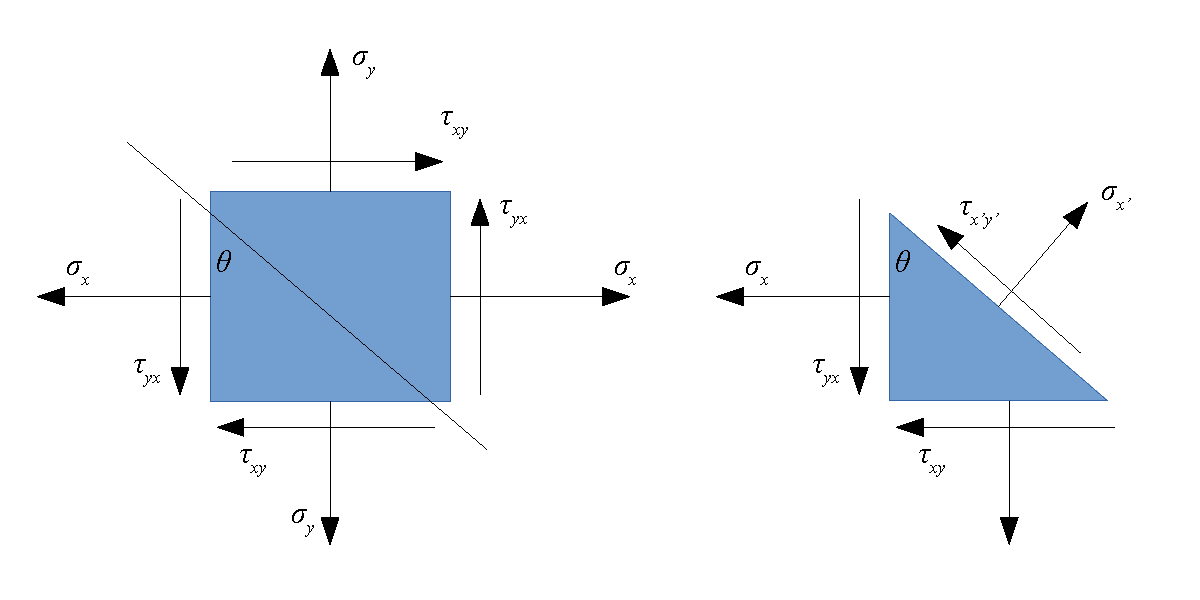
\includegraphics[scale=0.8]{pictures/Static-body-load-analysis/stress-transformation}
  \caption{Derivation of stress transformation equation by cutting element at an angle.}
  \label{fig: stress transformation}
\end{figure}

\paragraph{Normal and Shear Stress Components} The element is sectioned into a right-angle triangle with an angle of $\theta$ on the top as in the figure below. The resulting normal and shear stress on the newly sectioned side can be determined using equation of force equilibrium as

\[ \begin{gathered}
  \sum F_{x'}  = 0; \hfill \\[1em]
  \begin{split}
    \sigma_{x'}\Delta A - (\tau_{xy}\Delta A\sin \theta )\cos \theta  &- (\sigma_y\Delta A\sin \theta )\sin \theta  \\
    &- (\tau_{xy}\Delta A\cos \theta )\sin \theta  - (\sigma_x\Delta A\sin \theta )\cos \theta  = 0
  \end{split} \nonumber \\[0.5em]
  \sigma_{x'} = \sigma_x\cos^2\theta  + \sigma_y\sin^2\theta  + 2\tau_{xy}\sin \theta \cos \theta  \\[1em]
  \sum F_{y'}  = 0; \hfill \\ 
  \tau_{x'y'} = (\sigma_x - \sigma_y)\sin \theta \cos \theta  + \tau_{xy}(\cos^2\theta  - \sin ^2\theta ) \\ 
\end{gathered} \]

Once we know $\sigma_{x’}, \sigma_{y’}$ can be obtained simply by substituting $\theta$ with 90 + $\theta$

\[\sigma_{y'} = \sigma_x\sin^2\theta  + \sigma_y\cos^2\theta  - 2\tau_{xy}\sin \theta \cos \theta \]

If we know the stress components for all possible orientations of faces through a point, we say that we know the \emph{state of stress} at a point.

\subsection{Mohr’s Circle for Stress Transformation}

The stress transformation can be made easier to understand through the use of a graphical representation. However, first we have to rewrite stress transformation using double angle formulas.

\[\begin{gathered}
  \sigma_{x'} = \sigma_x\cos^2\theta  + \sigma_y\sin^2\theta  + 2\tau_{xy}\sin \theta \cos \theta  \hfill \\
  \sigma _{x'} = \frac{\sigma_x}{2}(1 + \cos 2\theta ) + \frac{\sigma_y}{2}(1 - \cos 2\theta ) + {\tau_{xy}}\sin 2\theta  \hfill \\
  \sigma_{x'} - \left( \frac{\sigma_x + \sigma_y}{2} \right) = \left( \frac{\sigma_x + \sigma_y}{2} \right)\cos 2\theta  + {\tau_{xy}}\sin 2\theta  \hfill \\ 
\end{gathered} \]

\[\begin{gathered}
  \tau_{x'y'} = (\sigma_y - \sigma_x)\sin \theta \cos \theta  + \tau_{xy}(\cos^2\theta  - \sin^2\theta ) \\
  \tau_{x'y'} = \left( \frac{\sigma_y - \sigma_x}{2} \right)\sin 2\theta  + \tau _{xy}\cos 2\theta \hfill \\ 
\end{gathered} \]

Square both expressions and add them together, we have

\[\begin{gathered}
    \left[ \sigma_{x'} - \left( \frac{\sigma_x + \sigma_y}{2} \right) \right]^2 + \tau_{x'y'}^2 = \left( \frac{\sigma_x - \sigma_y}{2} \right)^2\cos^2 2\theta  + 2\left( \frac{\sigma_x - \sigma_y}{2} \right)\tau_{xy}\cos 2\theta \sin 2\theta  + \tau_{xy}^2\sin^2 2\theta \\
    \hspace{4.7cm} + \left( \frac{\sigma_x - \sigma_y}{2} \right)^2 \sin^2 2\theta  + 2\left( \frac{\sigma_y - \sigma_x}{2} \right)\tau_{xy}\cos 2\theta \sin 2\theta  + \tau_{xy}^2\cos^2 2\theta \\ 
\end{gathered} \]

Simplifying the expression using trigonometry identities, we have

\[\left[ \sigma_{x'} - \left( \frac{\sigma_x + \sigma_y}{2} \right) \right]^2 + \tau_{x'y'}^2 = \left( \frac{\sigma_x - \sigma_y}{2} \right)^2 + \tau_{xy}^2\]

Since $\sigma_x$, $\sigma_y$, and $\tau_{xy}$ are known quantities for the problem, we can rewrite the expression as

\begin{equation}
  (\sigma_{x'} - \sigma_{avg})^2 + \tau_{x'y'}^2 = R^2
\end{equation}

Note that this equation represents a circle having radius $R$ and center on the $\sigma$ axis at point ($\sigma_{avg}$, 0).

\begin{figure}[h]
  \centering
  \begin{tikzpicture}
    \node at (-3,0) [anchor=west, draw, fill=SkyBlue, circle, minimum height=7cm](large){};
    \draw [<->] (-5,0) --++ (0:10) node[right]{$\sigma$};
    \draw [<->] (0,-5) --++ (90:10) node[above]{$\tau$};
    \node at (large.east) [below right] {$\sigma_1$};
    \node at (large.west) [below left] {$\sigma_2$};
    \draw (0,0) node[below left]{0};
    \draw [dashed](large.center) -- (large.south) node[below right](absolute){$(\tau_{x'y'})_{\max}$};
    \draw (large.center) --++ (50:3.5) node[above right]{$\sigma_x$} node(A){};
    \draw (large.center) --++ (-130:3.5) node[below left]{$\sigma_y$};
    \draw [dashed] (A.center) --++ (180:2.75) node[left]{$\tau_{xy}$};
    \draw (absolute.south) [out=-90, in=150] to ++(0.5,-0.5) node[right]{Maximum in-plane shear stress};
  \end{tikzpicture}
  % 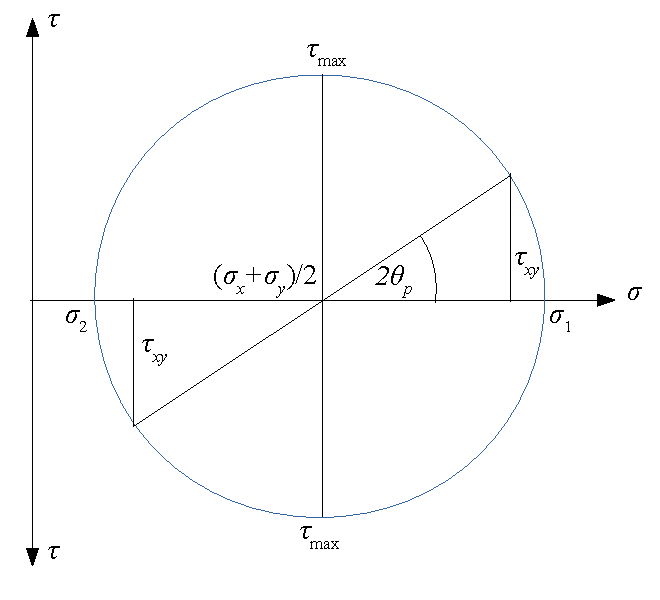
\includegraphics[scale=0.8]{pictures/Static-body-load-analysis/mohrs-circle}
  \caption{Mohr's circle and its representation of state of stress.}
  \label{fig: mohr's circle}
\end{figure}

This extremely useful graphical representation for stress transformation was developed by a German engineer Otto Mohr and is therefore called \emph{Mohr’s circle}.
The original state of stress can be determined by

\begin{equation}
  2\theta_p = \tan ^{-1}\frac{2\tau_{xy}}{\sigma_x - \sigma_y}
\end{equation}

where $\theta _p$ is called the \emph{principal direction}. And when determining the stress components in the material at angle $\alpha$ from its original coordinate system, simply draw the line from the center of the circle at angle $2\alpha$ from the original state to determine stress components at this new orientation.

\subsection{Principal stresses in 2D}

Considering the two points where the circle crosses the $\sigma$ axis, these two points are where the two normal stress components are at maximum and minimum. These two stresses are called the maximum and minimum principal stresses, respectively. We can represent them in terms of stresses in plane stress as

\begin{equation}
  \sigma_{1,2} = \frac{\sigma_x + \sigma_y}{2} \pm \sqrt {\frac{\sigma_x - \sigma_y}{2}^2 + \tau_{xy}^2}
\end{equation}

Also note that the shear stress component is zero in this orientation.

\subsection{Maximum Shear Stresses in 2D}

At the highest point of the circle represents the maximum shear stress and its orientation. We can represent the maximum shear stress in terms of stresses in plane stress as

\begin{equation} \label{eqn: max shear stress}
  \tau_{xy} = \sqrt {\left( \frac{\sigma_x - \sigma_y}{2} \right)^2 + \tau_{xy}^2}
\end{equation}

Since the angle between the principal stresses and maximum shear stress on Mohr’s circle is 90 degree, the actual angle between the principal stress plane and maximum shear stress plan is 45. Also note that the normal component stresses are equal to $\sigma_{avg}$.

\begin{example} State of stress of a plane stress element
  
  Determine the principal stresses, maximum shear stress, and the principal direction in this element 
  
  \begin{figure}[H]
    \centering
    \begin{tikzpicture}
      \node [draw, fill=LightBlue, regular polygon, regular polygon sides=4, minimum width=2cm](A){};
      \draw [->,very thick] (A.north) --++ (90:1) node[above]{$\sigma_y$ = 20 MPa};
      \draw [<-,very thick] (A.east) --++ (0:1) node[right]{$\sigma_x$ = -30 MPa};
      \draw [<-,very thick] (A.west) --++ (180:1);
      \draw [->,very thick] (A.south) --++ (-90:1);
      \node at (A.north west) [yshift=2mm] (B){};
      \draw [-left to, very thick] (B) --++ (0:1.3);
      \node at (A.south east) [xshift=2mm] (C){};
      \draw [-right to, very thick] (C) --++ (90:1.3) node[above right]{$\tau_{xy}$ = 25 MPa};
      \node at (A.north west) [xshift=-2mm] (D){};
      \draw [-right to, very thick] (D) --++ (-90:1.3);
      \node at (A.south east) [yshift=-2mm] (E){};
      \draw [-left to, very thick] (E) --++ (180:1.3) ;
    \end{tikzpicture}
    % 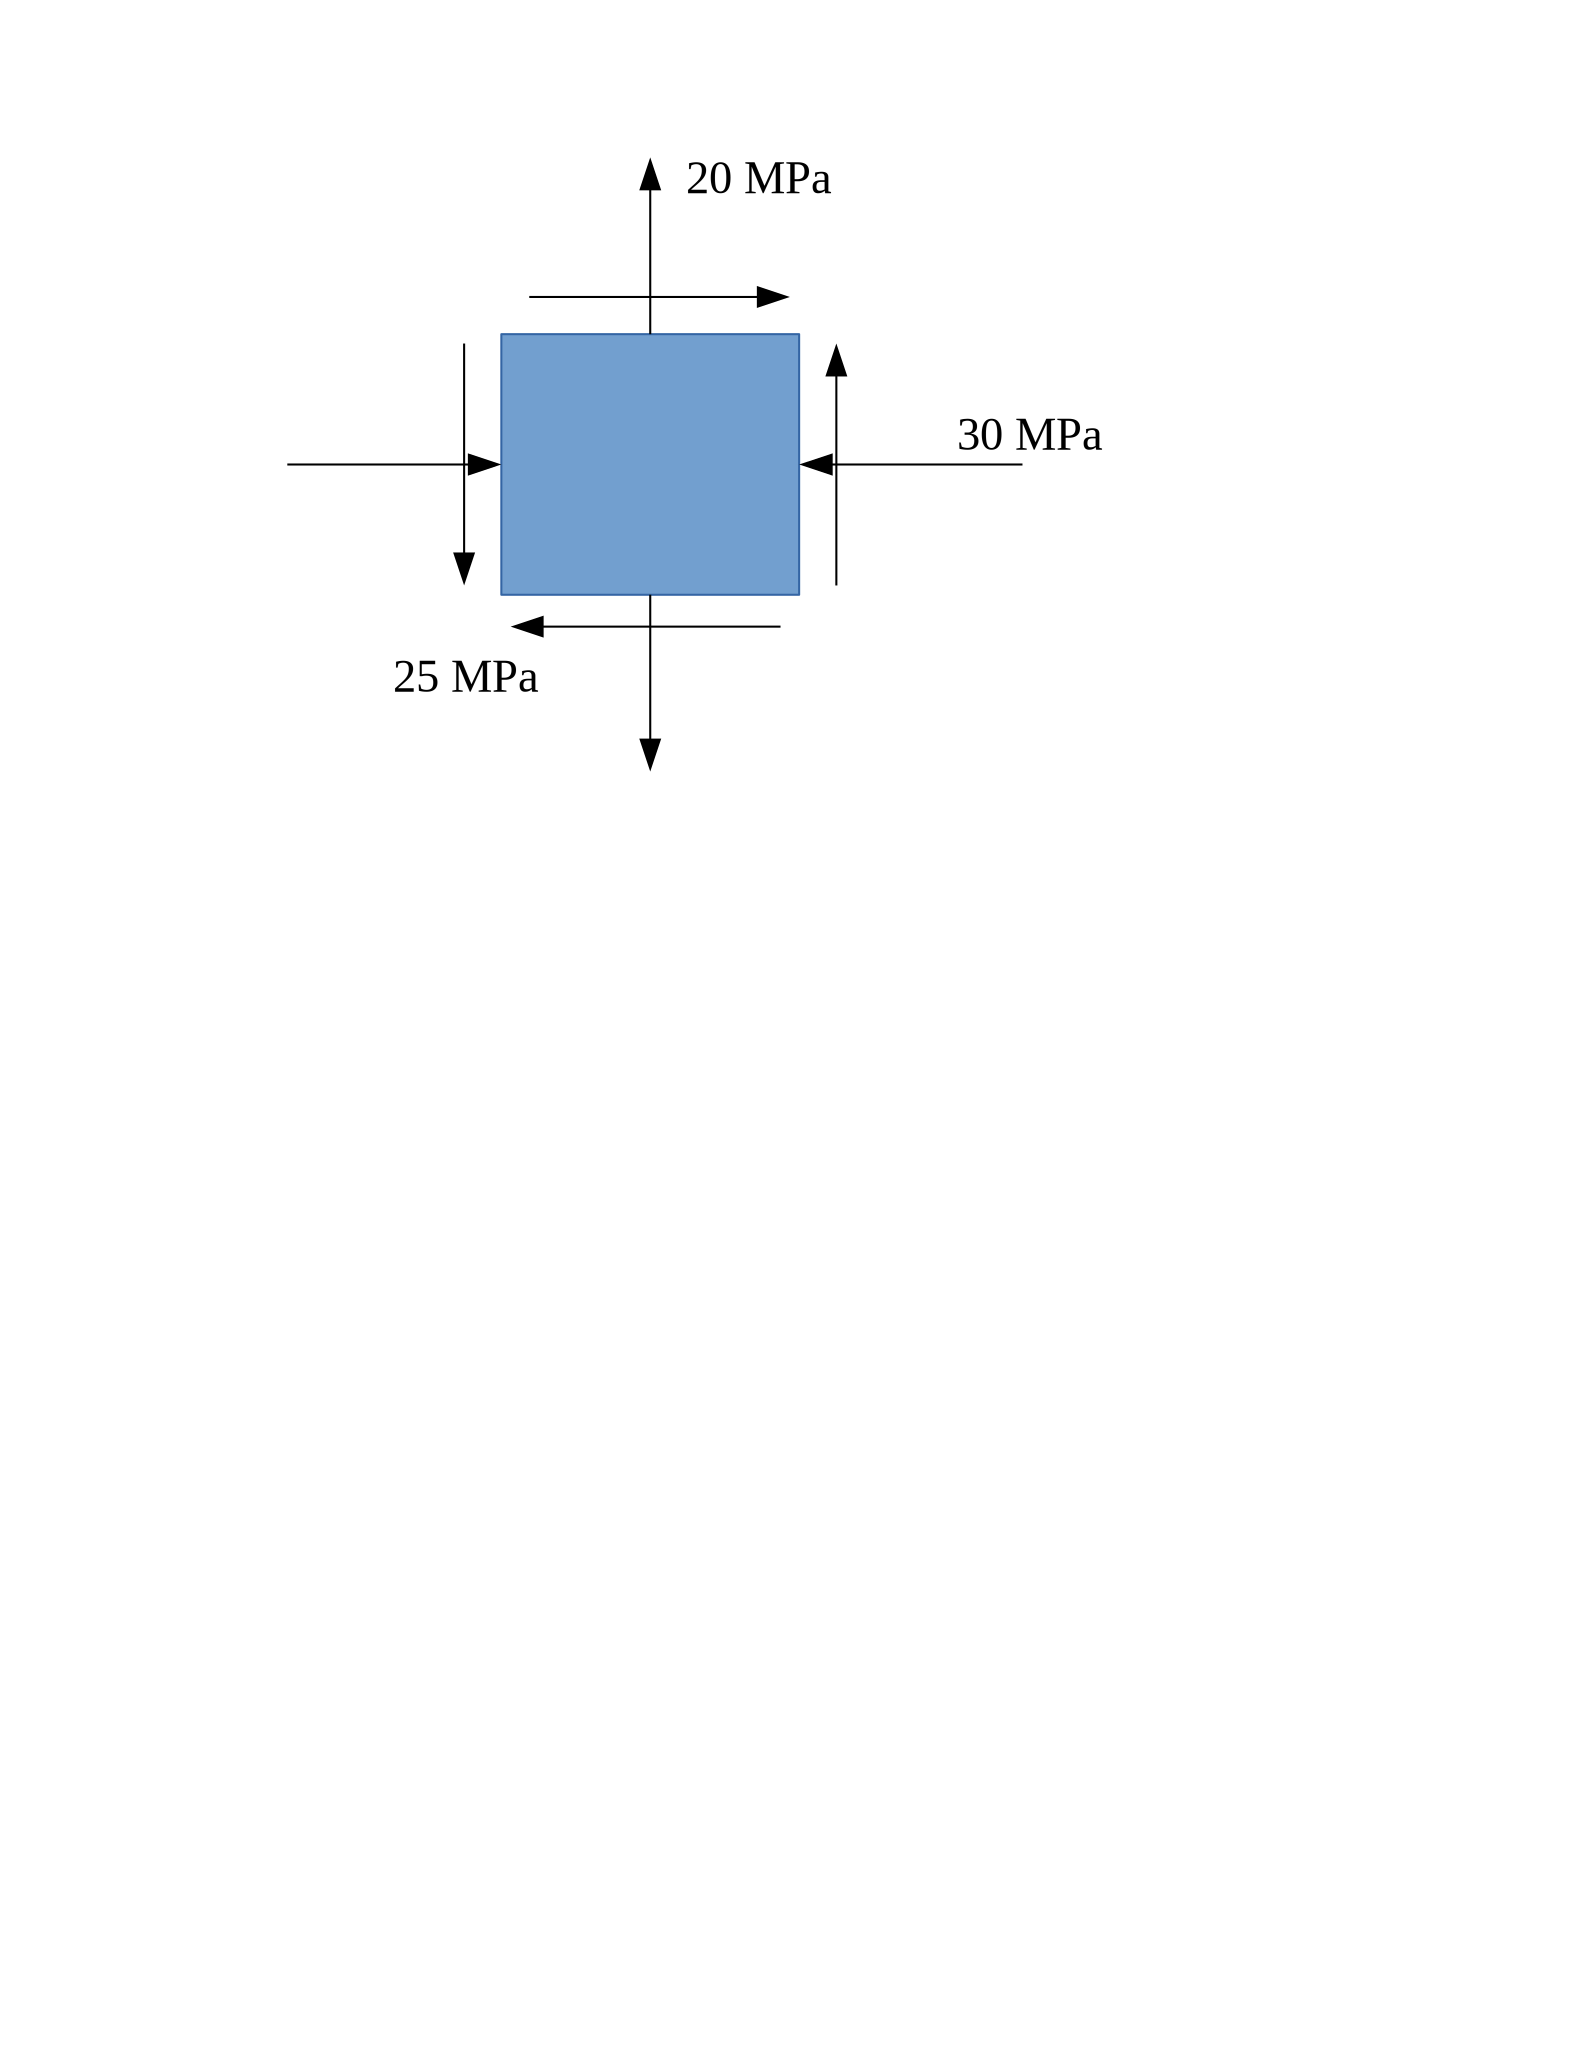
\includegraphics[scale=0.7]{pictures/Static-body-load-analysis/plane-stress-example}
  \end{figure}
\end{example}

\begin{solution}
  To determine the maximum shear stress, simply substitute the values into \cref{eqn: max shear stress} and obtain
  
  \[\begin{aligned}
      \tau_{xy} &= \sqrt {\left( \frac{\sigma_x - \sigma_y}{2} \right)^2 + \tau _{xy}^2}  \\ 
      &= \sqrt {\left( \frac{20 - ( - 30)}{2} \right)^2 + 25^2}  \\ 
      &= 35.4\text{ MPa}
    \end{aligned} \]
  
  The principal stresses are

  \[\begin{aligned}
      \sigma_{1,2} &= \frac{\sigma_x + \sigma_y}{2} \pm \sqrt {\frac{\sigma_x - \sigma_y}{2}^2 + \tau _{xy}^2}  \\ 
      &= \frac{20 - 30}{2} \pm 35.4 \\ 
      &= 30.4\text{ MPa}, \text{ } - 40.4\text{ MPa}
    \end{aligned} \]
  
  The principal direction is
  
  \[\begin{aligned}
      2\theta & = \tan^{-1}\frac{2\tau_{xy}}{\sigma_x - \sigma_y} \\ 
      &= 0.785 \\ 
      \theta  &= 0.393\text{ rad} \\ 
      &= 22.5^{\circ}
    \end{aligned} \]

\end{solution}

\begin{example} Analysis of a simply supported shaft under combined loadings.

\begin{figure}[H]
  \centering
  \begin{tikzpicture}[>=latex]
    \node [draw, top color=lightblue!60!Blue, bottom color=lightblue!60!Blue, middle color=lightblue, minimum height=6mm, minimum width=8cm](beam){};
    % supports
    \node at (beam.south east) [anchor=north, draw, fill=LightGrey, circle, minimum height=4mm, inner sep=0] (B){};
    \node at (beam.south west) [anchor=north, draw, fill=LightGrey, regular polygon, regular polygon sides=3, minimum height=5mm, inner sep=0] {};
    % dimensions
    \draw [|<->|] (beam.south west) ++ (-90:1) --++ (0:8) node[midway, above]{1 m};
    \draw [|<-] (beam.west) ++ (180:0.5) node[left, yshift=-1mm]{$r = 1$ cm} --++ (90:0.3); 
    \draw [|<-] (beam.south west) ++ (180:0.5) --++ (-90:0.3); 
    % loads
    \draw [<-, very thick] (beam.north) --++ (90:1) node[above]{1000 N};
    \draw [->, very thick] (beam.east) --++ (0:1) node[right]{10 kN};
  \end{tikzpicture}
\end{figure}

Determine the critical point location and its state of stress.
\end{example}
\begin{solution}
  It may not be obvious at first glance where the critical point on the shaft is. In that case, we may want to determine the critical point from each load and find common locations.

  For a midpoint-loaded simply-supported shaft, the critical point is in the middle ($x = 0.5$ m) on the top (compressive) and bottom (tensile) surface. The 10-kN tensile load does not provide any additional critical point as its resultant stress is uniform throughout the shaft. However, in this problem, the resultant tensile stress adds up with the tensile stress at the bottom surface and cancels with the compressive stress at the top surface. So only the top surface in the middle of the shaft is the critical point here.

  \begin{figure}[H]
    \centering
    \begin{tikzpicture}[>=latex]
      \node [draw, top color=lightblue, bottom color=lightblue, middle color=lightblue!20, minimum height=6mm, minimum width=8cm](beam){};
      % supports
      \node at (beam.south east) [anchor=north, draw, fill=LightGrey, circle, minimum height=4mm, inner sep=0] (B){};
      \node at (beam.south west) [anchor=north, draw, fill=LightGrey, regular polygon, regular polygon sides=3, minimum height=5mm, inner sep=0] {};
      \node at (beam.south) [anchor=south, draw, fill=red, rectangle, minimum height=1.5mm, minimum width=1.5mm, inner sep=0](critsouth){};
      \node at (beam.north) [anchor=north, draw, fill=red, rectangle, minimum height=1.5mm, minimum width=1.5mm, inner sep=0](critnorth){};
      \draw [<-] (critnorth.west) --++ (180:0.3);
      \draw [<-] (critnorth.east) --++ (0:0.3);
      \draw [->] (critsouth.west) --++ (180:0.3);
      \draw [->] (critsouth.east) --++ (0:0.3);
      % loads
      \draw [<-, very thick] (beam.north) --++ (90:1) node[above]{1000 N};
    \end{tikzpicture}
  \end{figure}

  \begin{figure}[H]
    \centering \hspace{2cm}
    \begin{tikzpicture}[>=latex]
      \node [draw, fill=red!80, minimum height=6mm, minimum width=8cm](beam){};
      % supports
      \node at (beam.south east) [anchor=north, draw, fill=LightGrey, circle, minimum height=4mm, inner sep=0] (B){};
      \node at (beam.south west) [anchor=north, draw, fill=LightGrey, regular polygon, regular polygon sides=3, minimum height=5mm, inner sep=0] {};
      \draw [->, very thick] (beam.east) --++ (0:1) node[right]{10 kN};
    \end{tikzpicture}
  \end{figure}

  \begin{figure}[H]
    \centering
    \begin{tikzpicture}[>=latex]
      \node [draw, top color=lightblue, bottom color=lightblue, middle color=lightblue!20, minimum height=6mm, minimum width=8cm](beam){};
      % supports
      \node at (beam.south east) [anchor=north, draw, fill=LightGrey, circle, minimum height=4mm, inner sep=0] (B){};
      \node at (beam.south west) [anchor=north, draw, fill=LightGrey, regular polygon, regular polygon sides=3, minimum height=5mm, inner sep=0] {};
      \node at (beam.south) [anchor=south, draw, fill=red, rectangle, minimum height=1.5mm, minimum width=1.5mm, inner sep=0](critsouth){};
      \node at (beam.north) [anchor=north, draw, fill=red, rectangle, minimum height=1.5mm, minimum width=1.5mm, inner sep=0](critnorth){};
      \draw [<-] (critnorth.west) --++ (180:0.3);
      \draw [->] (critnorth.west) ++ (180:0.35) --++ (180:0.2);
      \draw [<-] (critnorth.east) --++ (0:0.3);
      \draw [->] (critnorth.east) ++ (0:0.35) --++ (0:0.2);
      \draw [->] (critsouth.west) --++ (180:0.3);
      \draw [->] (critsouth.west) ++ (180:0.35) --++ (180:0.2);
      \draw [->] (critsouth.east) --++ (0:0.3);
      \draw [->] (critsouth.east) ++ (0:0.35) --++ (0:0.2);
    \end{tikzpicture}
  \end{figure}
  To determine the state of stress, we must first determine resultant stresses from axial load and bending. For axial load, we have

  \begin{align*}
    \sigma_a &= \frac{F}{A} \\
             &= \frac{10000}{\pi (0.01)^2} \\
             &= 31.8 \text{ MPa}
  \end{align*}

  For bending, we have
  \begin{align*}
    \sigma_b &= \frac{My}{I} \\
             &= \frac{1000(1)(0.01)}{4 \dfrac{\pi}{4}(0.01)^4} \\
             &= 318 \text{ MPa}
  \end{align*}

  As mentioned earlier, the directions of both of these stresses are along the length of the shaft, so we can add them up,  giving the final state of stress as 318 + 31.8 = 349.8 MPa.

\end{solution}
  
\section{Stress Concentration}

In cases where the cross section of the component under loading—axial, torsional, or bending—changes gradually, the formulas derived in previous sections still yield fairly accurate results. However, if the cross section changes abruptly, these equations cannot predict the local stress distribution near the discontinuity. Such local or peak stress is called stress concentration. This condition occurs around any discontinuities in a component’s cross section such as holes, notches, fillets, and threads. These features can lead to material failure by fracture or yield. While the stress and accompanying deformation near a discontinuity can be analyzed using the theory of elasticity, but application of either the finite element method or an experimental technique is more common. It is important to note that stress concentration is the primary cause of fatigue failures and static failures in brittle materials.

Experimental results show that the highest stress occurs in the narrowest part of the cross section close to the discontinuity, and its magnitude is significantly larger than the nominal, or average, stress. The ratio of the maximum stress to the nominal stress on the section is called the stress concentration factor, $K$, which can be expressed as

\begin{equation} \label{eqn: stress concentration}
  \sigma _{\max } = K\sigma _{nom}
\end{equation}

The factor usually depends on the geometry of the discontinuity; sharper, more sudden ones tend to cause higher stress concentration. Diagrams of readily available stress concentration factors can be found for various types of loadings (axial, torsional, and bending) and discontinuities (holes, fillets, notches, etc.). The diagrams included herein are by no means exhaustive.

It is important to remember that \cref{eqn: stress concentration} is valid as long as the values of $\sigma_{max}$ do not exceed the yield stress of the material, since the $K$s are based upon a linear stress-strain relationship. The discussion presented here is also only applicable to static loads.

\begin{figure}[H]
  \centering
  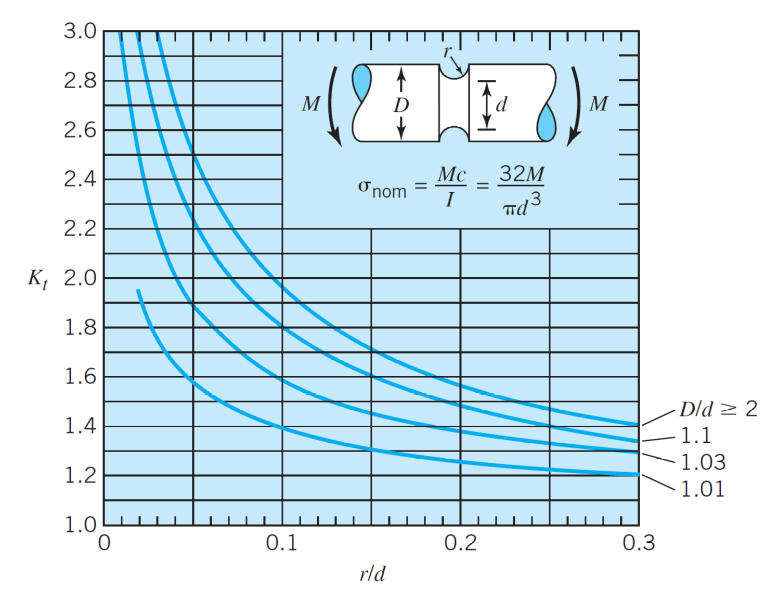
\includegraphics[scale=0.50]{pictures/Static-body-load-analysis/stress-conc-grooved-shaft}
  \caption{Stress concentration of a grooved shaft under bending \cite{juvinall2006fundamentals}}
  \label{fig: stress concentration of grooved shaft}
\end{figure}

\begin{figure}[H]
  \centering
  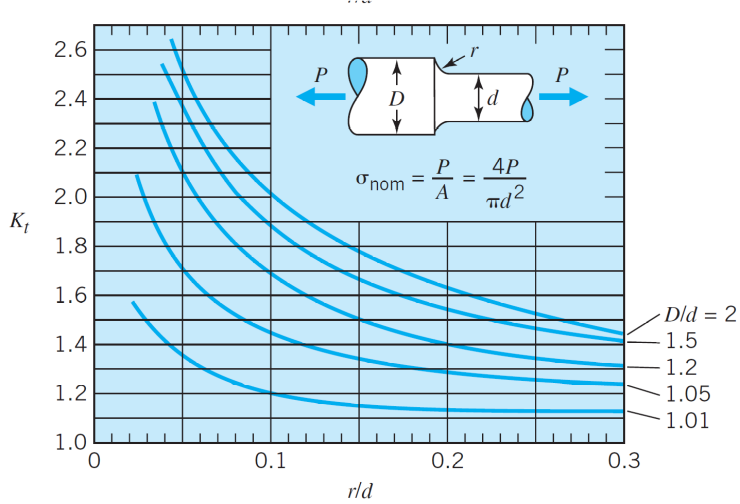
\includegraphics[scale=0.50]{pictures/Static-body-load-analysis/stress-conc-shaft-shoulder-fillet}
  \caption{Stress concentration factor of a shaft with shoulder fillet under axial loading \cite{juvinall2006fundamentals}}
  \label{fig: stress concentration of shaft with fillet}
\end{figure}

\begin{example} Determine the maximum load this multi-segment cantilever beam can take given that the beam material has $\sigma_{allow}$ = 150 MPa.

  \begin{figure}[H]
    \centering
    \begin{tikzpicture}[>=latex]
      \node [draw, top color=orange!50!white, bottom color=orange!50!white, middle color=orange!20!white, rectangle, minimum height=1.5cm, minimum width=3cm](left){};
      \draw [top color=orange!50!white, bottom color=orange!50!white, middle color=orange!20!white] (left.north east) arc (-160:-90:0.3) --++ (0:1.5) node(middle){} --++ (-90:1.1) --++ (180:1.5) arc (90:160:0.3);
      \draw [top color=orange!50!white, bottom color=orange!50!white, middle color=orange!20!white] (middle) arc (-160:-90:0.3) --++ (0:2) --++ (-90:0.7) node(force){} --++ (180:2) arc (90:160:0.3);
      \draw [->, ultra thick] (force.center) --++ (-90:1) node[right]{$P$};
      \draw [<-] (left.north east) --++ (45:0.75) node[right]{R3};
      \draw [<-] (middle.center) --++ (45:0.75) node[right]{R3};
      \node at (left.south east) [below] {A};
      \node at (left.south east) [xshift=1.7cm, below] {B};
      \node at (left.north) [above]{$\diameter 45 \times 200$};
      \node at (left.north east) [right]{$\diameter 30 \times 150$};
      \node at (middle.east) [right]{$\diameter 20 \times 250$};
    \end{tikzpicture}
  \end{figure}

  Use the following diagram for stress concentration factor.

  \begin{figure}[H]
    \centering
    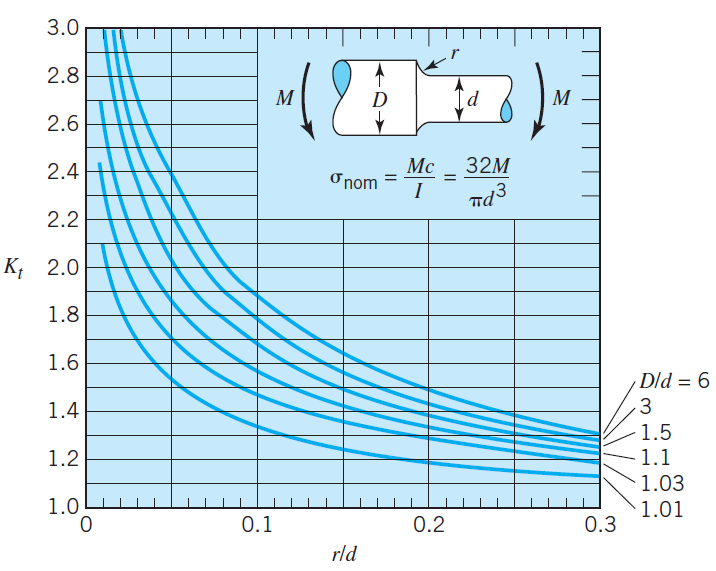
\includegraphics[scale=0.5]{pictures/Static-body-load-analysis/stress-conc-shaft-shoulder-fillet-bending}
  \end{figure}
\end{example}
\begin{solution}
  We must determine the stress at each candidate for critical point, modified by its corresponding stress concentration factor, leading to the actual critical point. Obviously, the candidates are at the corners where the change in cross-sectional area occur.

  Let us first consider the stress at point A, which is

  \begin{align*}
    \sigma_A &= K(\frac{r}{d}, \frac{D}{d}) \frac{32M}{\pi d^3} \\
             &= K(\frac{3}{30}, \frac{45}{30}) \frac{32[P(0.15 + 0.25)]}{\pi (0.03)^3} \\
             &= 1.68 \times 1.51 \times 10^5 P \\
             &= 2.54 \times 10^5 P
  \end{align*}

  A similar analysis can be done at point B.

  \begin{align*}
    \sigma_B &= K(\frac{r}{d}, \frac{D}{d}) \frac{32M}{\pi d^3} \\
             &= K(\frac{3}{20}, \frac{30}{20}) \frac{32P(0.25)}{\pi (0.02)^3} \\
             &= 1.5 \times 3.18 \times 10^5 P \\
             &= 4.77 \times 10^5 P
  \end{align*}

  Therefore, point B is the critical point of this beam. We can find the maximum applicable $P$ by setting the stress equal to the allowable stress.

  \begin{align*}
    \sigma_{allow} &= 150 \times 10^6 = 4.77 \times 10^5 P \\
    P &= 314 \text{ N}
  \end{align*}
\end{solution}

\begin{example} Analysis of De Havilland Comet Accident

  One of the most dire results of design without proper consideration for fatigue and stress concentration is the De Havilland Comet aircrafts which were in operation in 1952. While the aircraft design has many innovative features, they also influenced subsequent aircraft designers by two catastrophic failures. With some simplified calculations in this example, the sources and results of those failures can be illustrated.

  Less than two years into service, two of the Comets fell apart during ascent to cruise altitude. Investigators found that cracks started from the corner of a forward escape hatch. The figure below illustrated the location and geometry of the hatch.

  \begin{figure}[H]
    \centering
    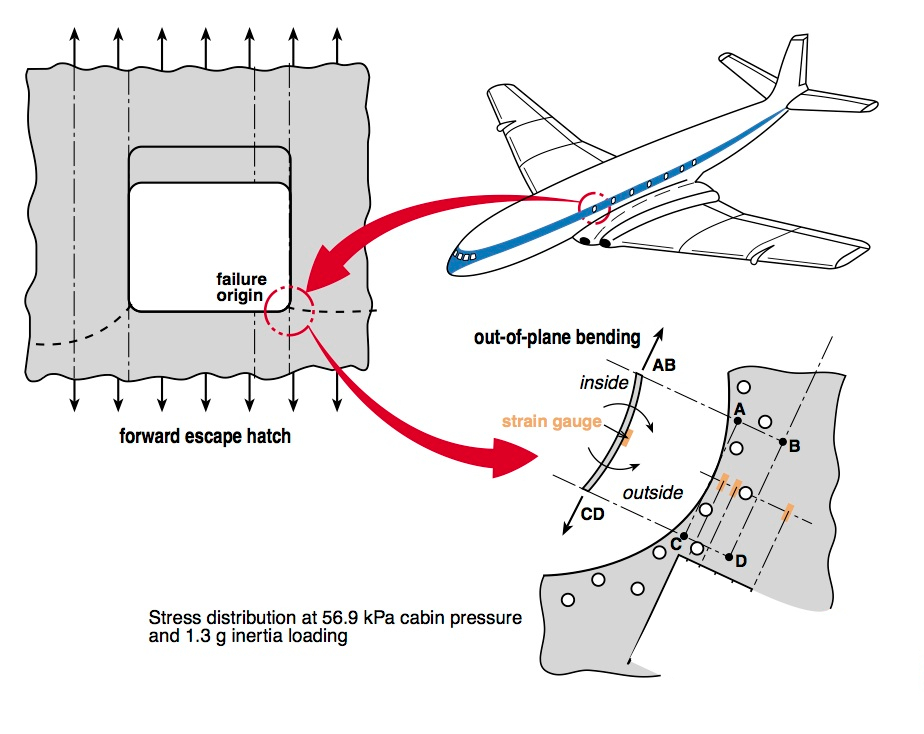
\includegraphics[width=0.7\textwidth]{pictures/Static-body-load-analysis/de-havilland-analysis}
  \end{figure}

  For simplification, assume the following material properties and geometry for the part.
  
  \begin{itemize}
  \item Fuselage: cylindrical pressure vessel thickness = 1 cm, radius = 3 m
  \item Cabin pressure: cycling between 0 and 57 kPa
  \item Radius of curvature = 5 cm
  \item Hole radius = 4 mm
  \item Wingspan = 35 m
  \item AISI1040: $S_y =$ 250 MPa, $S_{ut} =$ 400 MPa
  \item Mass at takeoff = 50000 kg
  \end{itemize}

  Use the following diagram for stress concentration factors.

  \begin{figure}[H]
    \centering
    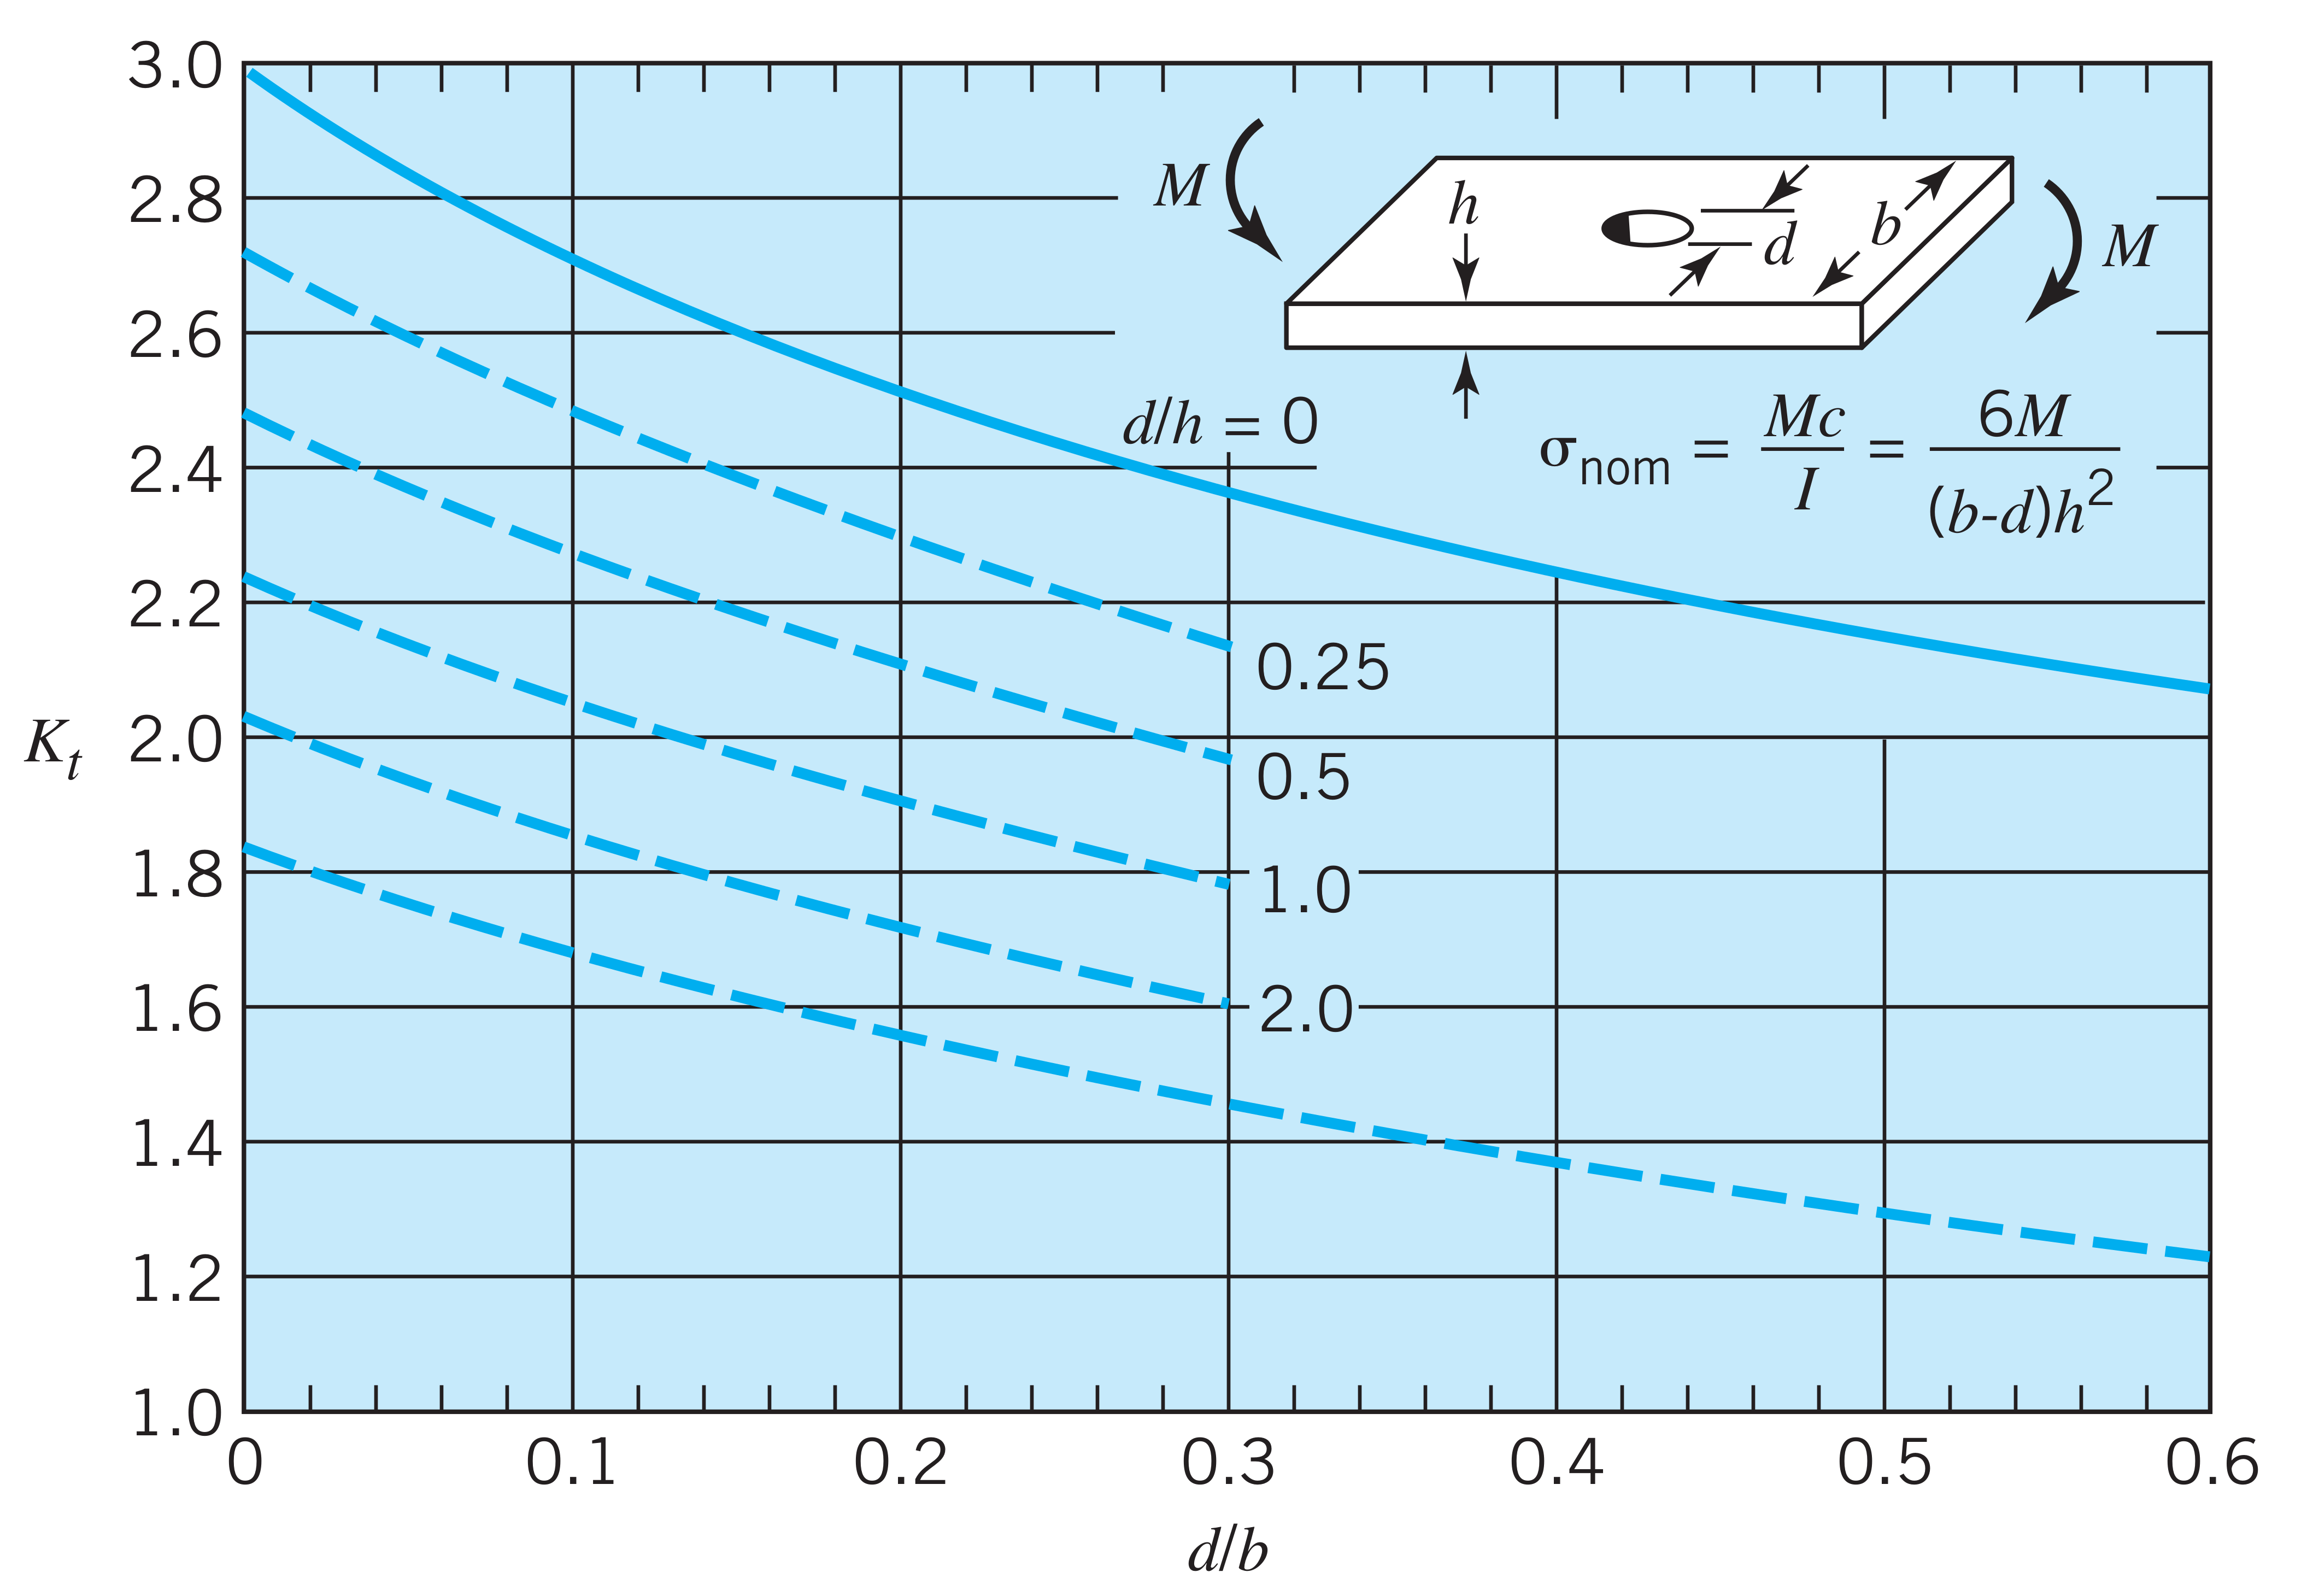
\includegraphics[width=0.6\textwidth]{pictures/Static-body-load-analysis/stress-conc-bending-plate}
  \end{figure}
  \begin{figure}[H]
    \centering
    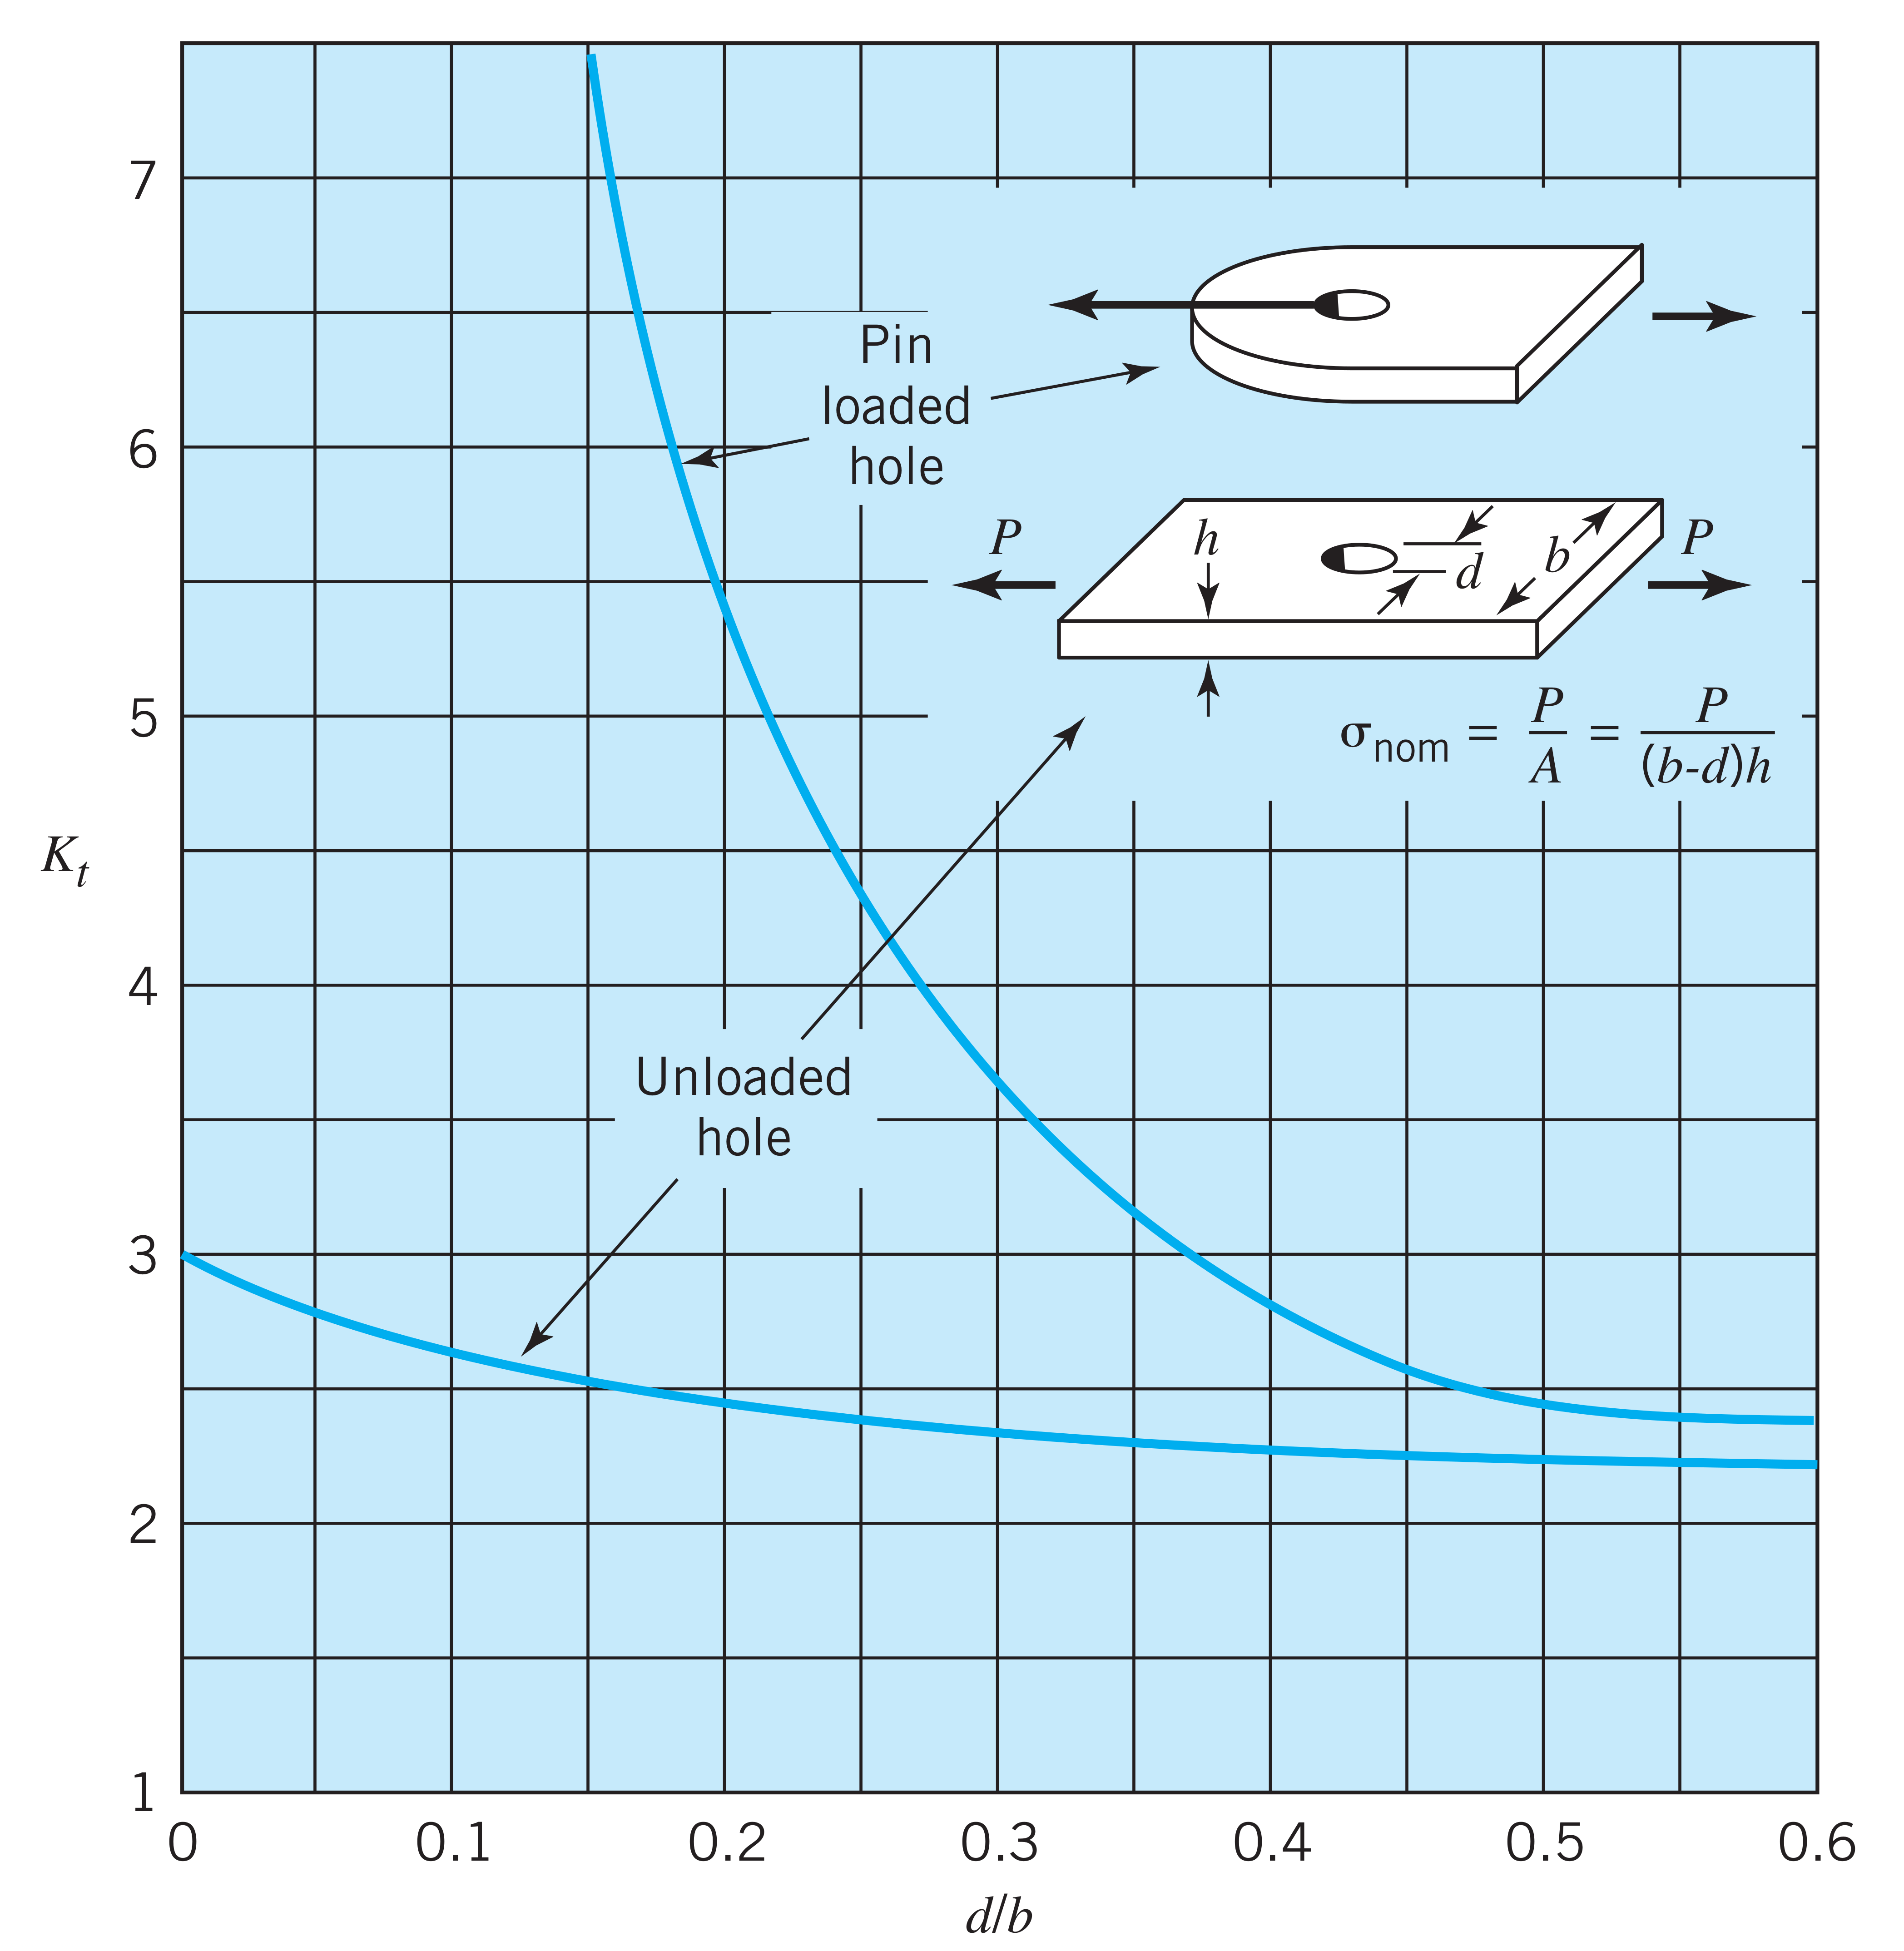
\includegraphics[width=0.6\textwidth]{pictures/Static-body-load-analysis/stress-conc-axial-plate}
  \end{figure}

  Determine the safety factor of the safety hatch at the corner.
\end{example}
\begin{solution}
  The stress is the fuselage can be considered as that of the wall of a cylindrical pressure vessel. The internal pressure during flight is 57 kPa and 0 when landed. The circumferential stress in the wall is 

  \begin{align*}
    \sigma_c &= \frac{pr}{t} \\
             &= \frac{(57 \times 10^3)(3)}{0.01} \\
             &= 17.1 \text{ MPa}
  \end{align*}

  Additionally, there is bending from the inertial load at 1.3g (1.3 times the weight). Simplify that the inertial load is divided equally between the two wings and that the divided load acts on the middle of each wing. We can subsequently calculate the bending moment at the exit hatch.

  \begin{align*}
    M &= 1.3(50000)(9.8) \left( \frac{35-3}{2} \right) \\
      &= 1.02 \times 10^7 \text{ N-m}
  \end{align*}
\end{solution}
\section*{Summary}

In this chapter, fundamentals of mechanics of materials are reviewed. To be able to analyze and properly design mechanical components, a designer must understand resultant stresses and deformations from applied loads. First, stress and deformation analysis for members under single type of loading—axial load, torsion, or bending—are discussed. Subsequently, analysis of multiaxial stress and combined loadings are detailed. Since mechanical components often have to take multiple loads simultaneously, we must understand the interactions between multiple loads and stresses.

Proficiency in these topics is crucial in the next chapter, which involves determining material failure under different loading conditions.

\section*{Exercises}

\begin{exercises}
  \exercise A compound bar consists of four brass wires of 2.5 mm diameter and one steel wire of 1.5 mm diameter. Determine
  
  \begin{figure}[H]
    \centering
    \begin{tikzpicture}
      \node at (0,0) [rectangle, fill=Grey, minimum height=0.25cm, minimum width=7cm](A){};
      \node at (A.north) [anchor=south, rectangle, fill=LightGrey, minimum height=0.25cm, minimum width=7cm](B){};
      \node at (B.north) [anchor=south, rectangle, fill=LightGrey, minimum height=0.25cm, minimum width=7cm]{};
      \node at (A.south) [anchor=north, rectangle, fill=LightGrey, minimum height=0.25cm, minimum width=7cm](C){};
      \node at (C.south) [anchor=north, rectangle, fill=LightGrey, minimum height=0.25cm, minimum width=7cm]{};
      \node at (A.west) [anchor=east, pattern=north west lines, minimum height=2cm, minimum width=1cm]{};
      \node at (A.east) [right] {$ \Bigg\}\rightarrow$ 500 N};
    \end{tikzpicture}
  \end{figure}
  
  \begin{enumerate}
  \item the stresses in each of the wires when the bar supports a load of 500 N, assuming all the wires are of equal lengths.
  \item the ‘equivalent’ or ‘combined’ modulus for the compound bar and its total extension if it is initially 0.75 m long.
  \end{enumerate}
  For brass $E_{br}$ = 100 GPa and for steel $E_{st}$ = 200 GPa.
  \exercise A compound bar is constructed from three bars 50 mm wide by 12 mm thick fastened together to form a bar 50 mm wide by 36 mm thick. The middle bar is of aluminum alloy for which $E_a$ = 70 GPa $\alpha_a$ = 23 $\times$ 10$^{-6}$ C$^{-1}$ and and the outside bars are of brass with $E_b$ = 100 GPa $\alpha_b$ = 20 $\times$ 10$^{-6}$ C$^{-1}$.

    \begin{figure}[H]
    \centering
    \begin{tikzpicture}
      \node at (0,0) [rectangle, fill=Grey, minimum height=0.25cm, minimum width=7cm](A){};
      \node at (A.north) [anchor=south, rectangle, fill=lightblue, minimum height=0.25cm, minimum width=7cm](B){};
      \node at (A.south) [anchor=north, rectangle, fill=lightblue, minimum height=0.25cm, minimum width=7cm](C){};
      \node at (A.west) [anchor=east, pattern=north west lines, minimum height=1cm, minimum width=0.2cm]{};
      \node at (A.east) [anchor=west, pattern=north west lines, minimum height=1cm, minimum width=0.2cm]{};
    \end{tikzpicture}
  \end{figure}
  
  \begin{enumerate}
  \item If the bars are initially fastened at 18 C and the temperature of the assembly is raised to 50 C, determine the stresses set up in the brass and the aluminum.
  \item What will be the changes in these stresses if an external compressive load of 15 kN is applied to the compound bar at the higher temperature?
  \end{enumerate}
  
  \exercise A solid shaft, 100 mm diameter, transmits 75 kW at 150 rev/min. Determine

    \begin{figure}[H]
    \centering
    \begin{tikzpicture}
      \node (0,0) [cylinder, draw,fill=lightblue, minimum height=8cm, minimum width=1cm]{};
      \draw[->>, very thick] (4,0) -- ++ (0:2) node[midway]{\AxisRotator[rotate=180]} node[right]{75 kW};
      \draw (5,1) node{150 rev/min};
      \draw[|<->|] (-4.2,-0.5) -- ++ (90:1) node[below left]{100 mm};
    \end{tikzpicture}
  \end{figure}
  
  \begin{enumerate}
  \item The value of the maximum shear stress in the shaft and the angle of twist per meter of the shaft length if $G$ = 80 GPa.
  \item The maximum torque the shaft could carry without exceeding the same maximum shear stress, if the shaft has now been bored so that its inner diameter is 60 mm in order to reduce weight.
  \end{enumerate}
  \exercise Determine the dimensions of a hollow shaft with a diameter ratio of 3:4 which is to transmit 60 kW at 200 rev/min. The maximum shear stress in the shaft is limited to 70 MPa and the angle of twist is 3.8 degree in a length of 4 m. The shaft material has $G$ = 80 GPa.
  \exercise A circular bar ABC, 3 m long, is rigidly fixed at its ends A and C. The portion AB is 1.8 m long and of 50 mm diameter and BC is 1.2 m long and of 25 mm diameter. If a twisting moment of 680 Nm is applied at B, determine the values of the resisting moments at A and C and the maximum stress in each section of the shaft. What will be the angle of twist of each portion? The shaft material has $G$ = 80 GPa.
  \exercise Determine the principal stresses, maximum shear stresses, and principal direction in each of these elements
  
  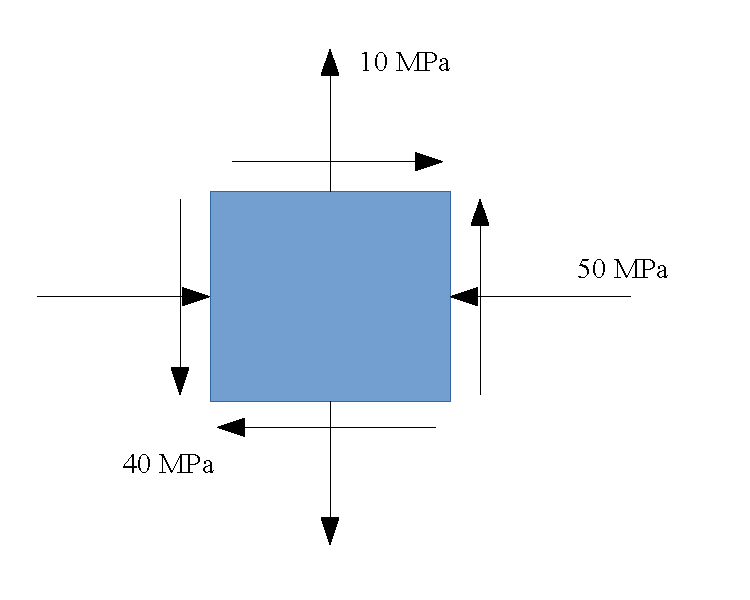
\includegraphics[scale=0.7]{pictures/Static-body-load-analysis/plane-stress-exercise1}
  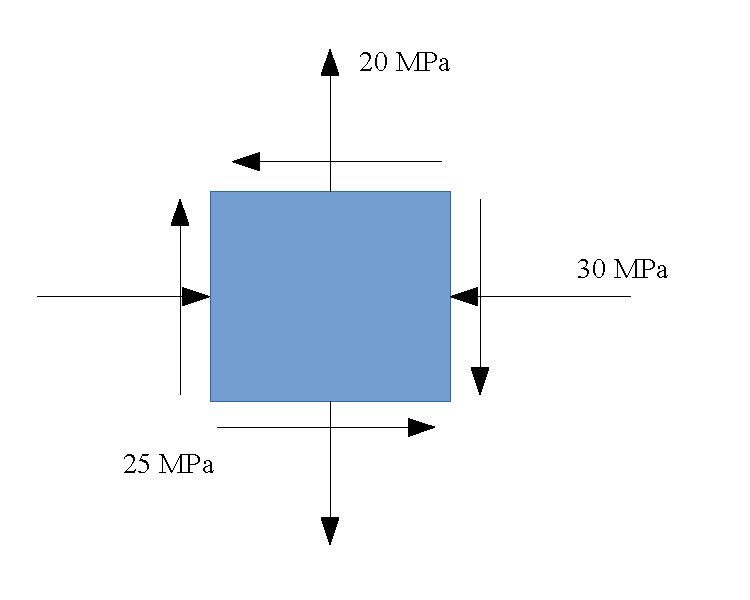
\includegraphics[scale=0.7]{pictures/Static-body-load-analysis/plane-stress-exercise2} \\
  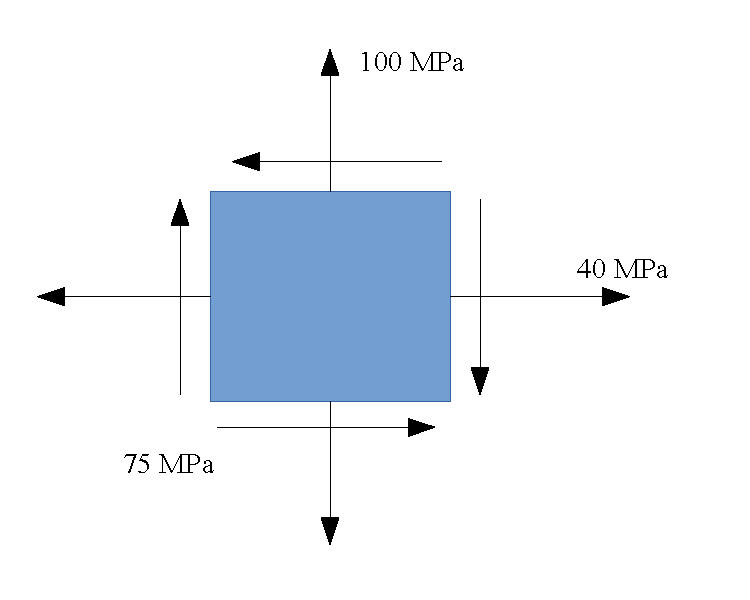
\includegraphics[scale=0.7]{pictures/Static-body-load-analysis/plane-stress-exercise3}
\end{exercises}

%%%%%%%%%%%%%%%%%%%%%%%%%%%%%%%%%%%%%%%%%%%%%%%%%%%%%%%%%%%%%%%%%%%%%%%%%%%%%%%%%%%%%%%%%%%%%%%%%%%%%%%%%%%%%%%%%%%%%%%%%%%%%%%%%%%%%%%%%%%%%%%%%%%%%%%%%%%%%%%%%%%%%%%%%%%%%%%%%%%%%%%%%%%%%%%%%%%%%%%%%%%%%%%%%%%%%%%%%%%%%%%%%

\chapter{Introduction to Theories of Failure}

Material failures occur when solid materials lose their strength due to external loads. In this section, we will discuss theories that predict the failure of materials due to multiple types of loadings—multiaxial, repeated, or compressive. These theories are used to determine the allowable stresses reported in design codes. Keep in mind that no single theory can apply to all materials under all situations, and therefore we must also be able to apply the appropriate theory to the appropriate situation.

\section{Yield and Fracture}

In uniaxial state of stress, the material behavior during yield is relatively simple and can be explained by yield stress criteria. However, more generally, we must apply failure criteria under a multiaxial state of stress. The study of the materials that yield is known as plasticity theory. We only limit ourselves to the first third of plasticity theory—the prediction of yield initiation.

A yield criterion can be any descriptive statement that defines conditions under which yielding will occur. It may be expressed in terms of specific quantities, such as stress state, the strain state, a strain energy quantity, or others. To develop a yield function, the components of the multiaxial stress state are combined into a single quantity known as the effective stress . The effective stress is then compared with the yield stress , in some appropriate form, to determine if yield has occurred.

\subsection{Maximum shear stress theory (Tresca criteria)}

The most common cause of yielding of a ductile material is slipping, which occurs due to shear stress. If we make a specimen into a highly polished thin strip and subject it to a simple tension test, we can see that the slip planes will occur approximately 45 degree with the axis of the strip. This actually coincides with the direction of maximum shear stress in a uniaxial stress loading, indicating that ductile materials yield due to shear stress. The maximum shear stress in a material that is loaded to its shear stress is $\tau_{max} = S_y / 2$ where the yield stress is determined from a simple tension test.

For application we will express the absolute maximum shear stress in terms of the principal stresses. If the two in-plane principal stresses have the same sign (both compressive or both tensile), the failure will occur out of plane and so

\begin{equation}
  \tau _{\max } = \frac{\sigma _{\max }}{2}
\end{equation}

However, if the principal stresses have opposite signs, then failure occurs in the plane and so

\begin{equation}
  \tau _{\max } = \frac{\sigma_{\max } - \sigma _{\min }}{2}
\end{equation}

Using these equations, we can express the maximum shear stress theory for plane stress for any two in-plane principal stresses by the following criteria

\begin{equation}
  \begin{array}{l l}
    \begin{gathered}
      \left| \sigma_1 \right| \leqslant S_y \hfill \\
      \left| \sigma_2 \right| \leqslant S_y \hfill \\ 
    \end{gathered}  &\text{when } \dfrac{\sigma _1}{\sigma _2} > 0  \\[20pt]
    \left| \sigma _1 - \sigma _2 \right| \leqslant S_y &\text{when } \dfrac{\sigma _1}{\sigma _2} < 0 \\ 
  \end{array}
\end{equation}

\begin{figure}[h]
  \centering
  \begin{tikzpicture}
    \draw [fill=lightblue] (0,-3) node[right]{$-S_y$} -- (3,0) node[below right]{$S_y$} -- (3,3) -- (0,3) node[left]{$S_y$} -- (-3,0) node[above left]{$-S_y$} -- (-3,-3) -- cycle;
    \draw [<->] (-4,0) --++ (0:8) node[right]{$\sigma_1$};
    \draw [<->] (0,-4) --++ (90:8) node[above]{$\sigma_2$};
    \end{tikzpicture}
  % 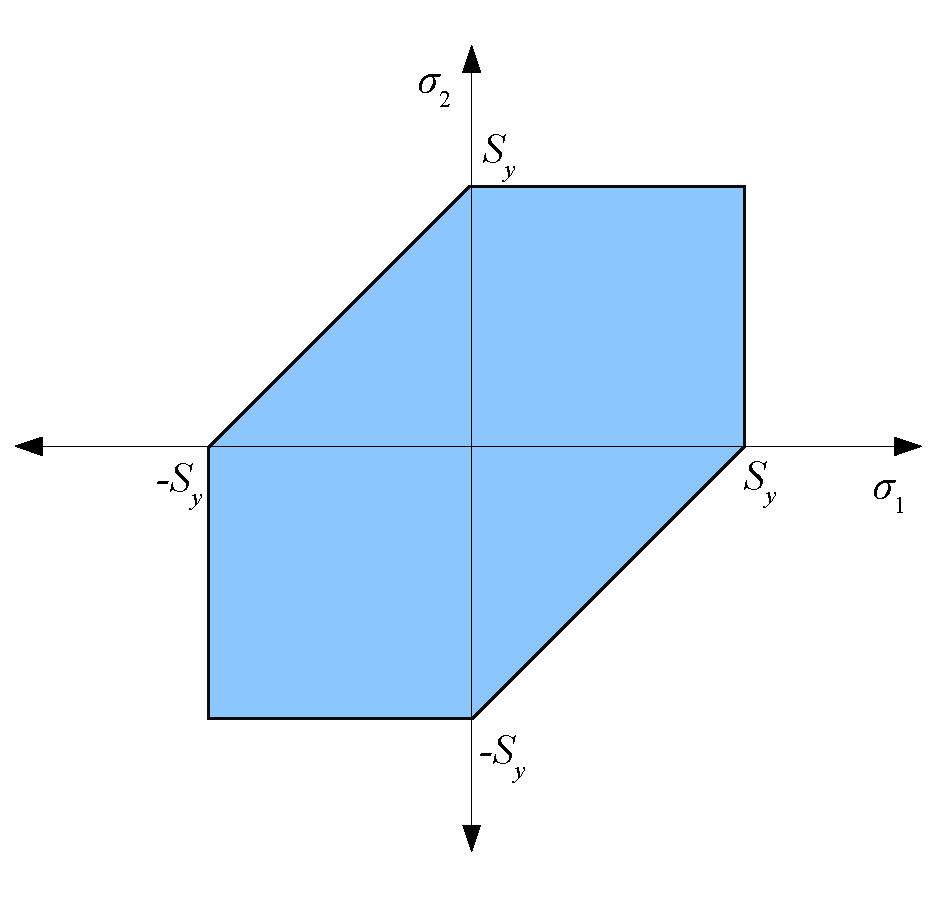
\includegraphics[scale=0.6]{pictures/Failure-theories/MSST-safe-zone}
  \caption{'Safe-zone' diagram for material under maximum shear stress criterion.}
  \label{fig: MSST safe zone}
\end{figure}

\Cref{fig: MSST safe zone} illustrates safe combinations of principal stresses under maximum shear stress criterion. Note the difference in the between the ‘safe areas’ in the first and third quadrants, which are squares, and second and fourth quadrants, which are triangles. In the first and third quadrants, the principal stresses are both tensile (first) or compressive (third). The resulting maximum in-plane shear stress is small. Therefore, the material will fail under normal stress instead of shear stress. In the second and fourth quadrants, the two principal stress signs are opposite, resulting in a large in-plane shear stress. In this case, the material is limited by the shear stress and the safe areas reflect this.

For design equations, the failure condition under MSST with safety factor Ns can be written as

\begin{equation}
  \begin{gathered}
    \begin{gathered}
        \left| \sigma_1 \right| > \frac{S_y}{N_s} \\
        \left| \sigma_2 \right| > \frac{S_y}{N_s}  \\ 
      \end{gathered}  \hspace{1.5cm} \text{when } \dfrac{\sigma _1}{\sigma _2} > 0 \\
      \left| {\sigma _1} - {\sigma _2} \right| > \frac{S_y}{N_s} \hspace{0.6cm} \text{when } \dfrac{\sigma_1}{\sigma_2} < 0
  \end{gathered}
\end{equation}

\subsection{Maximum distortion energy theory (Von Mises criteria)}

We know that when a material deforms by an external loading, it stores energy internally throughout its volume. The energy per unit volume of material is called the strain-energy density, and if the material is subjected to a uniaxial stress, the strain energy density can be written as

\[u = \frac{1}{2}\sigma \varepsilon \]

Similarly, if the material is subjected to three principal stresses then the total strain energy density becomes

\[u = \frac{1}{2}(\sigma_1\varepsilon_1 + \sigma_2\varepsilon_2 + \sigma_3\varepsilon_3)\]

If the material behaves in a linear-elastic manner, we can apply Hooke’s law, which transforms the equation to

\begin{equation} \label{eqn: distortion energy density}
  u = \frac{1}{2E}\left[\sigma_1^2 + \sigma_2^2 + \sigma_3^2 - 2\nu (\sigma_1\sigma_2 + \sigma_1\sigma_3 + \sigma_2\sigma_3)\right]
\end{equation}

This strain energy density can be considered as the sum of two parts, one part representing the energy needed to cause a volume change of the element with no change in shape, and the other representing the energy needed to distort the element. The energy stored in the form of volume change is a result of the average principal stress $\sigma_{avg} = \sigma_1 + \sigma_2 + \sigma_3$, since this stress causes equal principal strains in the material. The remaining portion of the stress $\sigma_1 - \sigma_{avg}$, $\sigma_2 - \sigma_{avg}$, $\sigma_3 - \sigma_{avg}$ causes the energy of distortion.

Experimental evidence has shown that materials do not yield when subjected to a uniform (hydrostatic) stress. M. Huber proposed that yielding in ductile material occurs when the \emph{distortion energy} per unit volume of the material equals or exceeds the distortion energy per unit volume of the same material when it is subjected to yielding in a simple tension test. This is called the \emph{maximum distortion energy theory}.
To obtain the distortion energy per unit volume, we substitute the distortion stresses into \cref{eqn: distortion energy density}. Expanding and simplifying, we have that

\[u_d = \frac{1 + \nu}{6E}\left[ (\sigma_1 - \sigma_2)^2 + (\sigma _2 - \sigma_3)^2 + (\sigma_3 - \sigma_1)^2 \right]\]

For uniaxial tension test, at yield, we have

\[(u_d)_y = \frac{1 + \nu}{3E}S_y^2\]

Since the theory requires that the distortion energy density be the same as the distortional energy from multiaxial stress state, we have

\begin{equation}
  (\sigma_1 - \sigma_2)^2 + (\sigma_2 - \sigma_3)^2 + (\sigma_3 - \sigma_1)^2 = 2S_y^2
\end{equation}

Or in the case of plane or biaxial stress, we have

\begin{equation}
  \sigma_e^2 = \sigma_1^2 - \sigma_1\sigma_2 + \sigma_2^2 = S_y^2
\end{equation}

This equation represents an elliptical curve. Once the state of stress of a material falls outside the ellipse, the material is said to have failed.
In comparison the maximum distortion energy theory is slightly more aggressive in terms of yield prediction, as shown in \cref{fig: MDET safe zone}.

\begin{figure}[h]
  \centering
  \begin{tikzpicture}
    \node [draw, ellipse, fill=lightblue, minimum width=7cm, minimum height=4.5cm, rotate=45](el){};
    \node at (el.north east)[left, xshift=-5mm]{$S_y$};
    \node at (el.south east)[below, yshift=-5mm]{$S_y$};
    \node at (el.north west)[above left, yshift=5mm]{$-S_y$};
    \node at (el.south west)[right, xshift=5mm]{$-S_y$};
    \draw [<->] (-4,0) --++ (0:8) node[right]{$\sigma_1$};
    \draw [<->] (0,-4) --++ (90:8) node[above]{$\sigma_2$};
  \end{tikzpicture}
  % 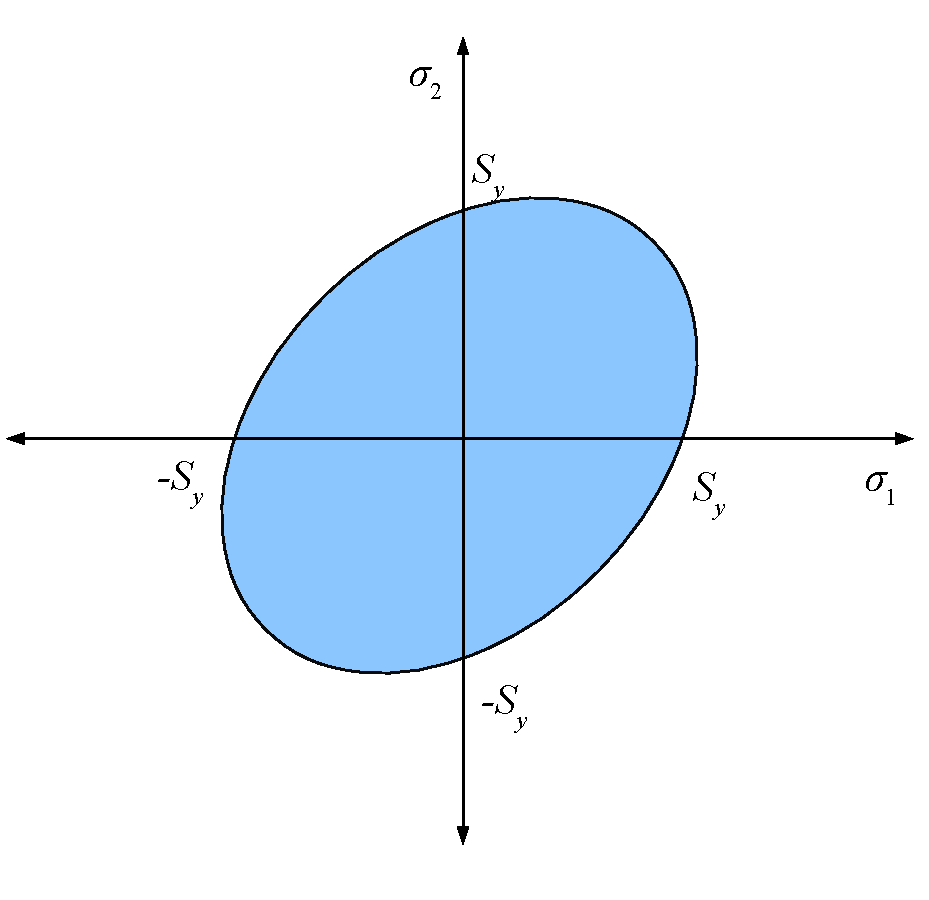
\includegraphics[scale=0.6]{pictures/Failure-theories/MDET-safe-zone}
  \caption{'Safe-zone' diagram for material under maximum distortion energy criterion.}
  \label{fig: MDET safe zone}
\end{figure}

The safety factor according to the criterion can be written as

\begin{equation}
  N_s(\text{MDET}) = \frac{S_y}{\sigma_e}
\end{equation}

\begin{example} Failure of a ductile plane-stress element

  A plane stress element having $\sigma_x = 50a$ MPa, $\sigma_y = 30a$ MPa and $\tau_{xy} =  25a$ MPa. If under uniaxial test, the material fails when the normal stress is 70 MPa, determine the maximum the value a that will cause the material to fail if it follows

  \begin{figure}[H]
    \centering
    \begin{tikzpicture}[>=latex]
      \node [draw, fill=LightBlue, regular polygon, regular polygon sides=4, minimum width=2cm](A){};
      \draw [->,very thick] (A.north) --++ (90:1) node[above]{$\sigma_y = 30a$ MPa};
      \draw [->,very thick] (A.east) --++ (0:1) node[right]{$\sigma_x = 50a$ MPa};
      \draw [->,very thick] (A.west) --++ (180:1);
      \draw [->,very thick] (A.south) --++ (-90:1);
      \node at (A.north west) [yshift=2mm] (B){};
      \draw [-left to, very thick] (B) --++ (0:1.3);
      \node at (A.south east) [xshift=2mm] (C){};
      \draw [-right to, very thick] (C) --++ (90:1.3) node[above right]{$\tau_{xy} = 25a$ MPa};
      \node at (A.north west) [xshift=-2mm] (D){};
      \draw [-right to, very thick] (D) --++ (-90:1.3);
      \node at (A.south east) [yshift=-2mm] (E){};
      \draw [-left to, very thick] (E) --++ (180:1.3) ;
    \end{tikzpicture}
  \end{figure} 

    \begin{enumerate}
  \item Maximum shear stress criterion
  \item Maximum distortion energy criterion
  \end{enumerate}
\end{example}

\begin{solution}

  First, the uniaxial test indicates the material’s yield stress, which is 70 MPa. In either case, to determine the maximum a, we have to determine the element’s principal stresses

  \[\begin{gathered}
      \sigma_{1,2} = \frac{\sigma_x + \sigma_y}{2} \pm \sqrt {\left( \frac{\sigma_x - \sigma_y}{2} \right)^2 - \tau _{xy}^2}  \\ 
      = \frac{50a + 30a}{2} \pm \sqrt {\left( \frac{50a - 30a}{2} \right)^2 + (25a)^2}  \\ 
      = a\left[ 10 \pm \sqrt {10^2 + 25^2} \right] \\ 
      = 37a \text{, } - 17a \\ 
    \end{gathered} \]
  
  \begin{enumerate}
  \item For maximum shear stress criterion, since the two principal stresses are of opposite signs, we know that the maximum stress is in-plane. We can apply equation so that
    
    \[\begin{gathered}
        \sigma_1 - \sigma_2 = S_y \hfill \\
        (37 - ( - 17))a = 70 \hfill \\
        a = 1.3 \hfill \\ 
      \end{gathered} \]
    
  \item For maximum distortion energy theory, we have that
    
    \[\begin{gathered}
        (\sigma_1 - \sigma_2)^2 + (\sigma_2 - \sigma_3)^2 + (\sigma_3 - \sigma_1)^2 = 2S_y^2 \\ 
        (37a - ( - 17a))^2 + ( - 17a)^2 + ( - 37a)^2 = 2(70)^2 \\ 
        4574a^2 = 9800 \\ 
        a = 1.46 \\ 
      \end{gathered} \]
    \end{enumerate}
\end{solution}

\subsection{Ductile Coulomb-Mohr theory}

Not all materials have the same compressive and tensile strengths. For example, the yield strengths of magnesium alloys in compression is approximately 50 percent of their yield strength in tension. The ultimate strength of grey cast irons in compression, on the other hand, can be as large as 300-400\% of their tensile strengths.

Mohr’s theory uses the results of three tests: tension, compression, and shear to construct three Mohr’s circles describing the state of stress at yield under the corresponding tests. Tangential lines connect the circles on the top and bottom of the circles to define a failure envelope of the theory.

A variation of Mohr’s theory, called the \emph{Coulomb-Mohr theory} or the \emph{internal-friction theory}, assume the tangential lines are straight. With this assumption, only the tensile and compressive strengths are necessary. Consider the conventional ordering of the principal stresses such that $\sigma_1 > \sigma_2 > \sigma_3$. The theory simply reduces to 

\[\frac{\sigma_1}{S_{ut}} - \frac{\sigma_3}{S_{uc}} = 1\]

For plane stress, when the two principal stresses $\sigma_1 > \sigma_2 > 0$, the failure condition become

\[\sigma_1 > S_{ut}\]

When  $\sigma_1 > 0 > \sigma_2$, the condition becomes

\[\frac{\sigma_1}{S_{ut}} - \frac{\sigma_2}{S_{uc}} > 1\]

When  $0 > \sigma_1 > \sigma_2$, the condition becomes

\[\sigma_2 <  - S_{uc}\]

\begin{figure}[h]
  \centering
  \begin{tikzpicture}
    \draw [fill=lightblue] (1.5,1.5) -- (1.5,0) node[below right]{$S_{ut}$}-- (0,-3) node[right]{$S_{uc}$}-- (-3,-3) -- (-3,0) node[below left]{$S_{uc}$} -- (0,1.5) node[above left]{$S_{ut}$} -- cycle;
    \draw [<->] (-5,0) --++ (0:8) node[right]{$\sigma_1$};
    \draw [<->] (0,-5) --++ (90:8) node[above]{$\sigma_2$};
  \end{tikzpicture}
 % 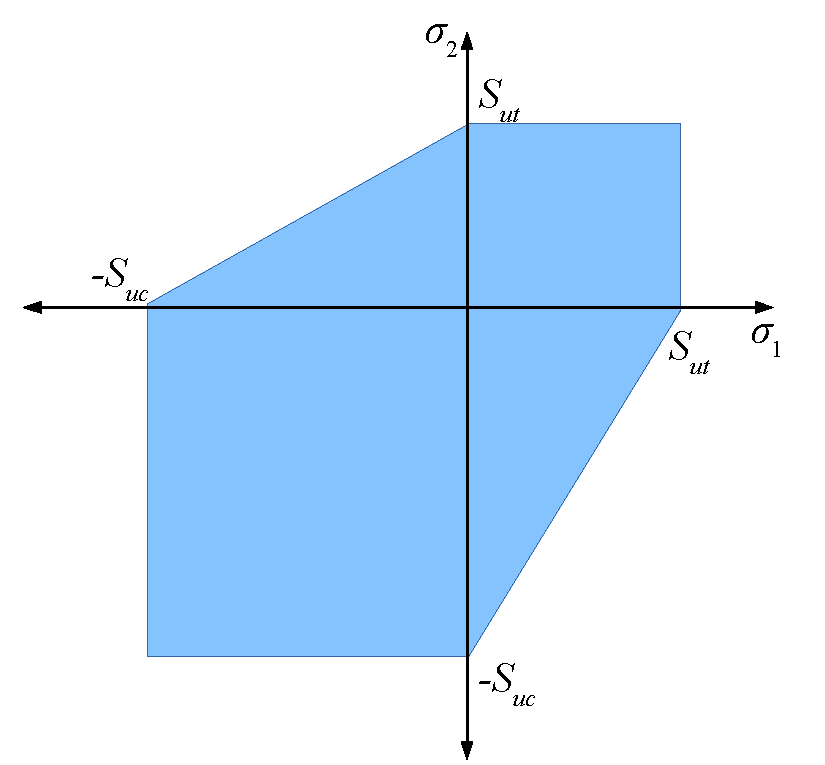
\includegraphics[scale=0.6]{pictures/Failure-theories/CM-ductile-safe-zone}
  \caption{`Safe-zone' diagram for material under ductile Coulomb-Mohr criterion.}
  \label{fig: Coulomb-Mohr ductile safe zone}
\end{figure}

For design equations, incorporating the safety factor $N_s$, simply divide all strengths by the factor.

\begin{equation}
  \begin{array}{l l l}
  \sigma_1 > \dfrac{S_{ut}}{N_s} & & \sigma_1 > \sigma_2 > 0 \\[10pt]
  \dfrac{\sigma_1}{S_{ut}} - \dfrac{\sigma_2}{S_{uc}} > \dfrac{1}{N_s} & & \sigma_1 > 0 > \sigma_2 \\[10pt]
    \sigma_2 <  -\dfrac{S_{uc}}{N_s} & & \sigma_2 < \sigma_1 < 0
  \end{array}
\end{equation}

\subsection{Maximum principal stress theory}

Also called \emph{Rankine’s criterion} or \emph{maximum normal stress criterion}, it states that yielding begins at a point in a member where the maximum principal stress reaches a value equal to the tensile yield stress $S_{ut}$. For example, assume that a nonzero principal stress acts at a point in the member. According to this criterion, yielding will occur when $\sigma_1$ or $\sigma_2$ reaches the value $S_{ut}$. If the material is subjected to plane stress, we require that

\[\begin{gathered}
    \left| \sigma _1 \right| \leqslant S_{ut} \hfill \\
    \left| \sigma _2 \right| \leqslant S_{uc} \hfill \\ 
  \end{gathered} \]

These equations are shown graphically in \cref{fig: MNST safe zone}. It is seen that if the stress coordinate at a point in the material falls on the boundary or outside the shaded area, the material is said to fracture.

\begin{figure}[h]
  \centering
  \begin{tikzpicture}
    \node [draw, rectangle, xshift=-1cm, yshift=-1cm, fill=lightblue, minimum height=6cm, minimum width=6cm](sq){};
    \draw [<->] (-5,0) --++ (0:8) node[right]{$\sigma_1$};
    \node at (sq.east) [yshift=7mm, right] {$S_{ut}$};
    \node at (sq.west) [yshift=7mm, left] {$S_{uc}$};
    \node at (sq.north) [xshift=1.3cm, above] {$S_{ut}$};
    \node at (sq.south) [xshift=7mm, below] {$S_{uc}$};
    \draw [<->] (0,-5) --++ (90:8) node[above]{$\sigma_2$};
  \end{tikzpicture}
  % 
\includegraphics[scale=0.6]{pictures/Failure-theories/MNST-safe-zone}
  \caption{'Safe-zone' diagram for material under maximum principal stress criterion.}
  \label{fig: MNST safe zone}
\end{figure}

Experimentally, the criterion has been found to be in close agreement with the behavior of brittle materials that have strain diagrams that are similar in both tension and compression. The safety factor according to the criterion can be expressed in design equations as

\begin{equation}
  \begin{array}{l l l}
  \sigma_1 > \dfrac{S_{ut}}{N_s} & & \sigma_1 > \sigma_2 > 0 \\[10pt]
  \left. \hspace{-0.23cm}
  \begin{array}{l l l}
    \sigma_1 & > & \dfrac{S_{ut}}{N_s} \\[10pt]
    \sigma_2 & < & -\dfrac{S_{uc}}{N_s}
    \end{array} \right\} & & \sigma_1 > 0 > \sigma_2 \\[10pt]
    \sigma_2 <  - \dfrac{S_{uc}}{N_s} & & \sigma _2 < \sigma _1 < 0
  \end{array}
\end{equation}

\subsection{Modified Coulomb-Mohr theory}

Over the years, various empirical theories have been proposed to modify the basic failure theories. Coulomb-Mohr theory was proposed to predict fracture in brittle materials for which compressive strength is much greater than tensile strength. The failure condition is identical to that of ductile Coulomb-Mohr theory. However, there are still discrepancies between the condition and experimental results. The theory, consequently, is slightly modified to better accommodate the results.

The modified Coulomb-Mohr theory failure condition can be expressed as

\begin{equation}
  \begin{array}{c c}
    \sigma_1 < \dfrac{S_{ut}}{N_s} &
      \begin{array}{c}
        \sigma_1 > \sigma_2 > 0 \\ 
        \sigma_1 > 0 > \sigma_2 \text{ and } \left| \dfrac{\sigma_1}{\sigma_2} \right| > 1 
      \end{array} \\[20pt]
    \dfrac{\sigma_1(S_{uc} - S_{ut})}{S_{uc}S_{ut}} - \dfrac{\sigma_2}{S_{uc}} >
      \dfrac{1}{N_s} & \sigma_1 > 0 > \sigma_2\text{ and }\left| \dfrac{\sigma_1}{\sigma_2} \right| < 1 \\[15pt]
    \sigma_2 <  -\dfrac{S_{uc}}{N_s} & \sigma_2 < \sigma_1 < 0 
  \end{array}
\end{equation} 

The failure condition diagram for the theory is illustrated in \cref{fig: MCM safe zone}

\begin{figure}[h]
  \centering
  \begin{tikzpicture}
    \draw [fill=lightblue] (1.5,1.5) -- (-1.5,1.5) -- (-4,0) -- (-4,-4) -- (0,-4) -- (1.5,-1.5) -- cycle;
    \node at (1.5,0) [below right]{$S_{ut}$};
    \node at (0,-4) [right]{$S_{uc}$};
    \node at (-4,0) [below left]{$S_{uc}$};
    \node at (0,1.5) [above right]{$S_{ut}$};
    \draw [<->] (-5.5,0) --++ (0:8) node[right]{$\sigma_1$};
    \draw [<->] (0,-5.5) --++ (90:8) node[above]{$\sigma_2$};
    \draw [dashed] (2,-2) -- (-2,2) node[left]{Shear diagonal};
  \end{tikzpicture}
  % 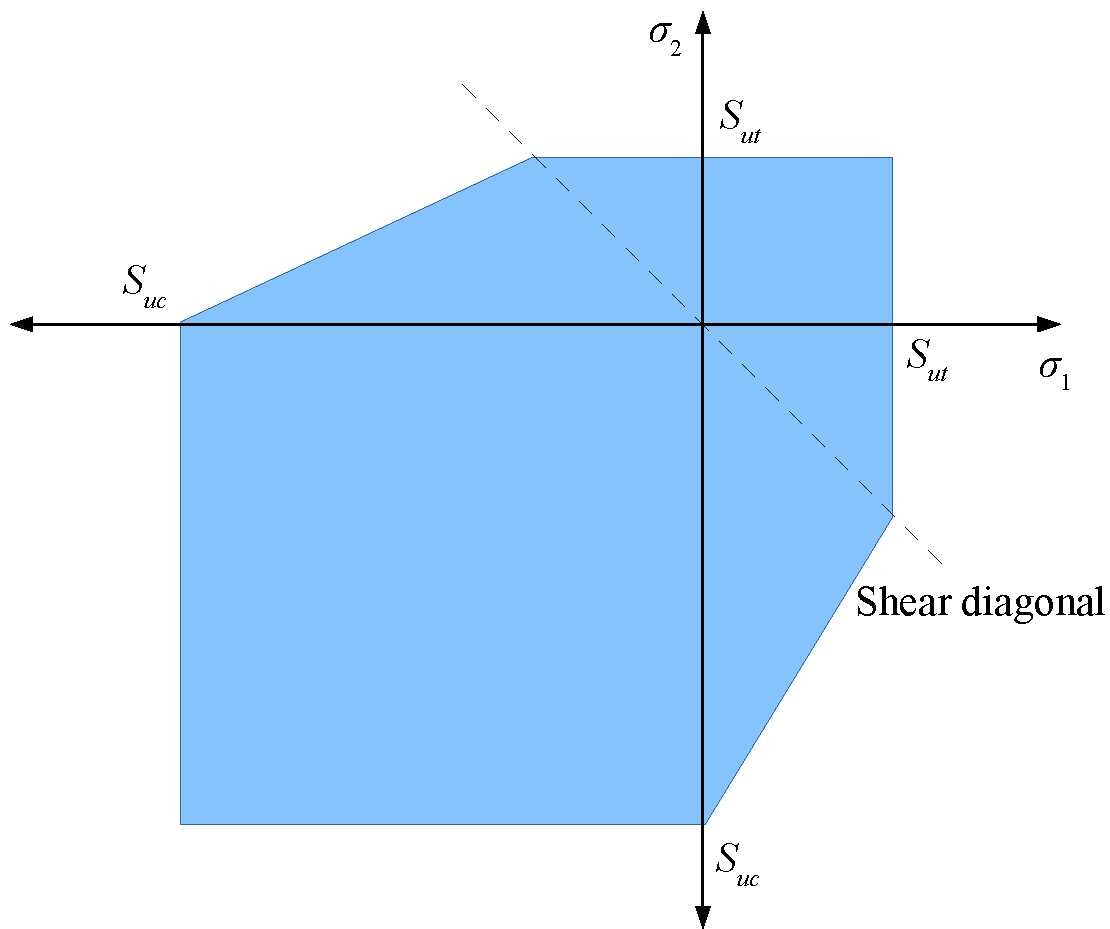
\includegraphics[scale=0.5]{pictures/Failure-theories/MCM-brittle-safe-zone}
  \caption{`Safe-zone' diagram for material under modified Coulomb-Mohr criterion.}
  \label{fig: MCM safe zone}
\end{figure}

\subsection{Criterion selection}

With an exception of a few, most ductile materials have the same tensile and compressive yield strengths. Therefore, \emph{maximum distortion energy theory} should be applicable. It is also more convenient than other maximum shear stress theory in that one mathematical expression applies to all states of stress regardless of the signs of the principal stresses.
For brittle materials, \emph{modified Coulomb-Mohr theory} shows the best fit to most experimental results and should be applied.

\section{Fatigue}

Fatigue has been defined as “the progressive localized permanent structural change that occurs in a material subjected to repeated or fluctuating strains at stresses having a maximum value less than the tensile strength of the material” (ASM, 1975). Fracture of a structural member as a result of repeated cycles of load or fluctuating loads in commonly referred to as a fatigue fracture or fatigue failure. The corresponding number of load cycles or the time during which the member is subjected to these loads before fracture occurs is referred to as the fatigue life.

The type of fatigue failure can be categorized base on the number of cycles before failure, $N$: high cycle fatigue for $N > 10^7$ cycles and low cycle fatigue for $N < 10^7$ cycles. High cycle fatigue is characterized by small elastic strains and can be captured by stress-based parameters. Low cycle fatigue, on the other hand, is characterized by large plastic strains and is captured by strain-based parameters.

To simplify the problem of fatigue failure, we can assume that the repeated loading causes the internal stress in the material to take a sinusoidal form, i.e.

\begin{figure}[h]
  \centering
  \begin{tikzpicture}[>=latex]
    \draw[<->] (-5,0) -- (5,0) node[right] {$t$}; 
    \draw[<->] (0,-1) -- (0,2) node[above] {$\sigma$};
    \draw[color=blue, domain=-4:4, samples=100]   plot (\x,{sin(3.5*\x r)+0.5})    node[right] {$\sigma = {\sigma _a}\sin 2\pi ft + {\sigma _m}$}; 
  \end{tikzpicture}
\end{figure}

\[\sigma  = \sigma _a\sin 2\pi ft + \sigma _m\]

where $f$ is the frequency of the load, $\sigma_a$ is the stress amplitude, and $\sigma_m$ is the mean stress.
When testing for material fatigue, it is common to test for the relationship between the exerted stress and the number of cycles before the specimen fails. This \emph{endurance} graph or $S-N$ graph, normally shows that as the alternating stress amplitude increases, the number of cycle the material can take before failure decreases. Some materials exhibit endurance limits--lower limits of stress amplitudes under which the materials no longer exhibit fatigue fracture. For other materials that do not exhibit endurance limits, it is customary to define the stresses to cause failure under a given number of cycle, say $N = 10^7$, as the \emph{endurance limit} or \emph{fatigue strength}, $S_e$.

\begin{figure}[h]
  \centering
  \begin{tikzpicture}[>=latex]
    %grid
    \draw[ultra thin,color=lightgray] (0,0) grid (10,6);
    %axes
    \draw[<->]  (0,6) node [left] {$\sigma_a$} -- (0,5) node[left]{$S_l$} -- (0,2) node[left]{$S_e$}
    -- (0,0) node[below] {$10^3$} --
    (2,0)  node[below]{$10^4$} -- (4,0) node[below]{$10^5$} -- (6,0) node[below]{$10^6$} --
    (8,0) node[below]{$10^7$} -- (10,0) node[right] {$N$};
    % Steel
    \draw[very thick, blue] (0,5) to (3.5,3) to [out=-28,in=-180] (8,2) node[above]{Steel} to (10,2);
    \draw[very thick, green] (0,5) to [out=-40,in=160] (6.5,1) node[below left]{Aluminum} to (9,0);
  \end{tikzpicture}
  \caption{A typical endurance diagram showing stress amplitude $\sigma_a$ vs number of cycles to failure $N$.}
  \label{fig: S-N diagram}
\end{figure}

Typically, steel exhibit this endurance limit. However, many aluminum alloys do not; there does not exist a minimum stress below which fatigue does not occur. This is why these aluminum alloys, though lighter, simply cannot replace steel in many machine design applications.

\subsection{Fatigue under zero mean stress}

When the load is completely reversed, resulting in zero mean stress ($\sigma_m = 0$), fatigue failure can mostly be described by stress amplitude. At the lower end of this spectrum where the number of cycles to failure $N = 10^3$, the stress amplitude that leads to failure is called the \emph{low cycle fatigue limit}, $S_l$, and can be approximated as

\begin{equation}
  S_l = \left\{
    \renewcommand{\arraystretch}{1.2}
    \begin{array}{ll}
      0.9 S_{ut} &\text{ for bending} \\
      0.75 S_{ut} &\text{ for axial} \\
      0.72 S_{ut} &\text{ for torsion}
    \end{array}
  \right.
\end{equation}

On the far end of the spectrum where $N = 10^7$, the stress amplitude is the \emph{endurance limit}, $S_e$, which can be approximated as

\begin{equation}
  S_e = \left\{
    \renewcommand{\arraystretch}{1.2}
    \begin{array}{ll}
      0.5 S_{ut} & \text{ for bending} \\
      0.45 S_{ut} &\text{ for axial} \\
      0.29 S_{ut} &\text{ for torsion}
    \end{array}
  \right.
\end{equation}

For stress amplitude between the two ends, the expected number of cycles, $N$, can be interpolated. The relationship between them can be written as

\begin{equation}
  \sigma_a = 10^cN^b
\end{equation}

where $c$ and $b$ are parameters that can be obtained from

\begin{align*}
  b &= - \frac{1}{3} \log \dfrac{S_l}{S_e} \\
  c &= \log \dfrac{S_l^2}{S_e}
\end{align*}

Parameter $b$ is between $-0.06$ to $-0.14$ for most metals.

\subsection{Fatigue under nonzero mean stress}

Nonzero mean stresses have a significant effect on the fatigue strength of a material. There have been several relations proposed to describe the effects of mean stress. Three of such relations are

\begin{enumerate}
\item Soderberg relation
  \begin{equation}
    \frac{\sigma_a}{S_e} + \frac{\sigma _m}{S_y} = \frac{1}{N_s}
  \end{equation}
\item Gerber relation
  \begin{equation}
    \frac{\sigma_a}{S_e} + \left( \frac{\sigma_m}{S_{ut}} \right)^2 = \frac{1}{N_s}
  \end{equation}
\item Goodman relation
  \begin{equation}
    \frac{\sigma_a}{S_e} + \frac{\sigma _m}{S_{ut}} = \frac{1}{N_s}
  \end{equation}
\end{enumerate}

where $\sigma_a$ is the stress amplitude, $S_e$ is the endurance limit, $S_y$ is the yield stress, $\sigma_m$ is the mean stress, and $S_{ut}$ is the ultimate tensile strength. For most metals, the Soderberg relation yields conservative estimates of critical stress amplitude. The Goodman relation gives reasonably good results for brittle materials, whereas it is conservative for ductile materials. The Gerber relation yields fairly good estimates for stress amplitude for ductile materials.

\begin{example} Fatigue failure of a rod under a periodic tensile load

  A cylindrical rod shall operate under a periodic tensile load as shown in the graph. Material of the rod is AISI1050 which has the following properties.
  Yield strength = 427 MPa
  Ultimate tensile strength = 748 MPa
  Modified endurance limit = 300 MPa
  Determine the suitable diameter of the rod. Use Soderberg line with $N_s$ = 3

  \begin{figure}[H]
    \centering
    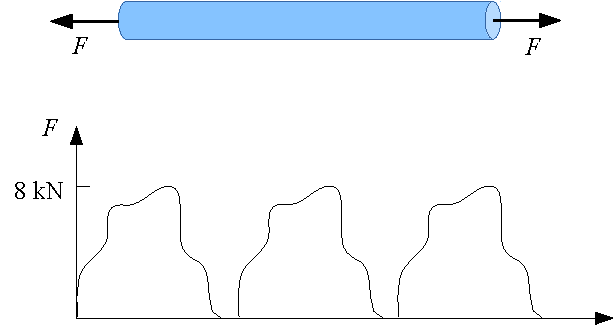
\includegraphics[scale=0.9]{pictures/Failure-theories/fatigue-example}
    % \caption{'Safe-zone' diagram for material under modified Coulomb-Mohr criterion.}
    % \label{fig: MCM safe zone}
  \end{figure}
\end{example}
\begin{solution}
    The safety factor of a member under alternate loading using the Soderberg line is as follows

    \[\frac{\sigma_a}{S_e} + \frac{\sigma_m}{S_y} = \frac{1}{N_s}\]

  The stress amplitude is simply the force amplitude divided by the cross sectional area of the rod.

  \[\sigma_a = \frac{(8000 + 0)/2}{\dfrac{\pi }{4}d^2} = \frac{16000}{\pi d^2}\]

  According to the Soderberg relation, we have

  \begin{gather*}
    \frac{\sigma_m}{S_y} + \frac{\sigma _a}{S_e} = \frac{1}{3} \\ 
    \dfrac{\dfrac{4000}{\dfrac{\pi }{4}d^2}}{427 \times 10^6} + \dfrac{\dfrac{16000}{\pi d^2}}{300 \times 10^6} = \frac{1}{3} \\[1em] 
    d^2 = 6.29 \times 10^{-5} \hfill \\
    d = 7.9 \times 10^{-3} = 7.9 \text{ mm} \hfill \\ 
  \end{gather*}
  Therefore, the rod’s diameter must be 7.9 mm.
\end{solution}

\section{Buckling} \label{section: buckling}

Whenever a member is designed, it is necessary that it satisfy specific strength, deflection, and stability requirements. The previous chapters we have discussed some of the methods used to determine the member’s strength and deflection, while assuming that the member was always in stable equilibrium. Some members, however, may be subjected to compressive loads, which, if sufficiently large, can cause the member to deflect laterally. To be more specific, long slender members subjected to an axial compressive force are called columns, and the lateral deflection that occurs is called buckling. Buckling of a column can lead to a sudden and often disastrous failure of a structure or mechanism, and therefore special attention must be given to the design of columns to prevent such problems.

The maximum axial load that a column can support is called the critical load, $P_{cr}$. Any additional loading will cause the column to buckle and therefore deflect laterally. Depending on the supports of a column, the critical load can vary.

\subsection{Ideal column with pin supports}

In this section we will determine the critical buckling load for a column that is pin-supported. The column to be considered is an \emph{ideal column}, meaning one that is perfectly straight before loading, is made of homogeneous material, and upon which the load is applied through the centroid of the cross section.
When the critical load $P_{cr}$ is reached, the column is on the verge of becoming unstable, so that a small lateral force $F$ will cause the column to remain in the deflected position when $F$ is removed. Any slight reduction in the load $P$ from Pcr will allow the column to straighten out, and any slight increase in $P$ beyond $P_{cr}$ will cause further increases in lateral deflection.
Whether or not a column will remain stable or become unstable when subjected to an axial load will depend on its ability to restore itself, which is based on its resistance to bending. Therefore, to determine the critical load and the buckled shape of the column, we will apply the equation for beam bending,

\[EI\frac{d^2v}{dx^2} = M\]

Recall that this equation assumes that the slope of the curve is small and that deflections occur only by bending. When the column is in its deflected position, the internal bending moment can be determined by using the method of sections. The bending moment in the beam is simply the product of the compressive load $P$ and the maximum deflection in the middle $v$. Note that the bending moment is negative, according to the sign convention used to establish equation so that $M = –Pv$. Thus equation becomes

  \begin{figure}[H]
    \centering
    \begin{tikzpicture}[>=latex]
      % beam and neutral axis
      \draw [lightblue, line width=10pt] (-4,0) node(A){} arc (110:70:14) node(B){};
      \draw [dashed] (-4,0) arc (110:70:14);
      % left support
      \node at (A.center) [anchor=east, draw, regular polygon, regular polygon sides=3, minimum height=4mm, inner sep=0, fill=LightGrey, shape border rotate=30](C){};
      \node at (A.center) [draw, circle, inner sep=1.5, fill=LightGrey]{};
      % right support
      \node at (B.center) [anchor=west, draw, regular polygon, regular polygon sides=3, minimum height=4mm, inner sep=0, fill=LightGrey, shape border rotate=-30](D){};
      \node at (B.center) [draw, circle, inner sep=1.5, fill=LightGrey]{};
      % wall
      \node at (D.east) [anchor=west,rectangle, pattern=north east lines, minimum height=2cm, minimum width=0.5cm]{};
      % force
      \draw [<-, line width=2pt] (C.west) -- ++ (180:1) node[left]{$P$};
      % horizontal level
      \draw [dashed] (A.center) -- (B.center);
      % vertical deflection
      \draw [<->] (A.center) ++ (3,0) --++ (90:0.75) node[midway, right]{$v$};
    \end{tikzpicture}
  \end{figure}
  
  \begin{gather*}
    EI\frac{d^2v}{dx^2} =  - Pv \\
    \frac{d^2v}{dx^2} + \left( \frac{P}{EI} \right)v = 0 
  \end{gather*}

This is a homogeneous second order linear differential equation with constant coefficients. The solution is of the form

\begin{equation} \label{eqn: gen solution}
  v = C_1\sin \left( \sqrt {\frac{P}{EI} x} \right) + C_2\cos \left( \sqrt {\frac{P}{EI}} x \right)
\end{equation}

Using the two boundary conditions that $v(x = 0) = 0$ and $v(x = L) = 0$, it can be determined that $C_2 = 0$ and

\[C_1\sin \left( \sqrt {\frac{P}{EI}} L \right) = 0\]

One way for this solution to be valid is for $C_1 = 0$, but this means that the column will remain straight since it leads to $v = 0$. This is a trivial solution and is not particularly interesting. The other, more interesting possibility is for 

\[\sin \left( \sqrt {\frac{P}{EI}} L \right) = 0\]

which is satisfied if

\begin{equation} \label{eqn: mode shape sub}
  \sqrt {\frac{P}{EI}} L = n\pi
\end{equation}

or

\begin{equation}
  P = \frac{n^2\pi^2EI}{L^2} \hspace{1cm}n = 1,2,3,...
\end{equation}

The smallest value of $P_{cr}$ is obtained when $n = 1$, so the \emph{critical load} for the column is therefore

\begin{equation}
  P_{cr} = \frac{\pi ^2EI}{L^2}
\end{equation}

This load is sometimes referred to as the \emph{Euler load}.

For the corresponding buckling mode shapes, substitute the expression in equation \cref{eqn: mode shape sub} into \cref{eqn: gen solution} along with other solved parameters, we have

\[v = C_2\sin \frac{n\pi x}{L}\]

Let us explore other buckling loads and their corresponding mode shapes. For $n = 2$, we have

$$ P = \frac{4 \pi^2 E I}{L^2} $$

and the mode shape is described by

$$ v = C_2 \sin \frac{2 \pi x}{L} $$

\begin{figure}[H]
  \centering
  \begin{tikzpicture}[>=latex]
    % beam and neutral axis
    \draw [lightblue, line width=10pt, smooth, domain=0:10] node(A){} plot (\x, {sin(2*pi*\x/10 r)}) node(B){};
    % \draw [dashed] (-4,0) arc (110:70:14);
    % left support
    \node at (A.center) [anchor=east, draw, regular polygon, regular polygon sides=3, minimum height=4mm, inner sep=0, fill=LightGrey, shape border rotate=30](C){};
    \node at (A.center) [draw, circle, inner sep=1.5, fill=LightGrey]{};
    % right support
    \node at (B.center) [anchor=west, draw, regular polygon, regular polygon sides=3, minimum height=4mm, inner sep=0, fill=LightGrey, shape border rotate=-30](D){};
    \node at (B.center) [draw, circle, inner sep=1.5, fill=LightGrey]{};
    % wall
    \node at (D.east) [anchor=west,rectangle, pattern=north east lines, minimum height=2cm, minimum width=0.5cm]{};
    % force
    \draw [<-, line width=2pt] (C.west) -- ++ (180:1) node[left]{$P$};
    % horizontal level
    \draw [dashed] (A.center) -- (B.center);
  \end{tikzpicture}
\end{figure}
  
And for $n=3$, the buckling load and corresponding mode shape are

$$ P = \frac{4 \pi^2 E I}{L^2} $$

$$ v = C_2 \sin \frac{2 \pi x}{L} $$
  
\begin{figure}[H]
  \centering
  \begin{tikzpicture}[>=latex]
    % beam and neutral axis
    \draw [lightblue, line width=10pt, smooth, domain=0:10] node(A){} plot (\x, {sin(3*pi*\x/10 r)}) node(B){};
    % \draw [dashed] (-4,0) arc (110:70:14);
    % left support
    \node at (A.center) [anchor=east, draw, regular polygon, regular polygon sides=3, minimum height=4mm, inner sep=0, fill=LightGrey, shape border rotate=30](C){};
    \node at (A.center) [draw, circle, inner sep=1.5, fill=LightGrey]{};
    % right support
    \node at (B.center) [anchor=west, draw, regular polygon, regular polygon sides=3, minimum height=4mm, inner sep=0, fill=LightGrey, shape border rotate=-30](D){};
    \node at (B.center) [draw, circle, inner sep=1.5, fill=LightGrey]{};
    % wall
    \node at (D.east) [anchor=west,rectangle, pattern=north east lines, minimum height=2cm, minimum width=0.5cm]{};
    % force
    \draw [<-, line width=2pt] (C.west) -- ++ (180:1) node[left]{$P$};
    % horizontal level
    \draw [dashed] (A.center) -- (B.center);
  \end{tikzpicture}
\end{figure}

For purposes of design, the critical load equation can also be written in a more useful form by expressing $I = Ar_g^2$, where $A$ is the cross-sectional area and $r_g$ is the \emph{radius of gyration} of the cross-sectional area. Thus,

\begin{gather*}
  P_{cr} = \frac{\pi^2EAr_g^2)}{L^2} \\ 
  \left( \frac{P}{A} \right)_{cr} = \frac{\pi ^2E}{(L/r_g)^2}
\end{gather*}

or

\begin{equation}
  \sigma_{cr} = \frac{\pi ^2E}{(L/r_g)^2}
\end{equation}

The geometric ratio $L/r_g$ is known as the \emph{slenderness ratio}. It is a measure of the column’s flexibility.

\subsection{Columns having various types of supports}

In some other cases where the columns are supported in some other way, so that the column’s ends may be restricted against rotations or deflection in different ways, determination of the buckling load on the column follows the same procedure. Take, for example, a column whose one end is fixed while the other is free. Assume that the compressive load is exerted onto the free end. The internal bending moment at an arbitrary section, whose lateral deflection is $v$, is $M = P(\delta – v)$. The differential equation for the deflection curve is

  \begin{figure}[H]
    \centering
    \begin{tikzpicture}[>=latex]
      % beam and neutral axis
      \draw [lightblue, line width=10pt] (-4,0) node(A){} arc (-110:-90:28) node[inner sep=0pt](B){};
      \draw [dashed] (-4,0) arc (-110:-90:28);
      % wall
      \node at (B.west) [anchor=west,rectangle, pattern=north east lines, minimum height=2cm, minimum width=0.5cm]{};
      % force
      \draw [<-, line width=2pt] (A.center) -- ++ (180:1) node[left]{$P$};
      % horizontal level
      \draw [dashed] (B.center) -- ++ (180:10);
      % vertical deflection and max deflection
      \draw [<->] (A.center)  --++ (-90:1.7) node[midway, right]{$\delta$};
      \draw [<->] (B.center)  ++ (-6.4,0) --++ (90:0.8) node[midway, right]{$v$};
    \end{tikzpicture}
  \end{figure}

\begin{gather*}
  EI\frac{d^2v}{dx^2} = P(\delta  - v) \\ 
  \frac{d^2v}{dx^2} + \frac{P}{EI}v = \frac{P}{EI}\delta  \\ 
\end{gather*}

Since this equation is nonhomogeneous, the solution consists of both a complementary and particular solutions.

\[v = C_1\sin \left( \sqrt {\frac{P}{EI}} x \right) + C_2\cos \left( \sqrt {\frac{P}{EI}} x \right) + \delta \]

Solving for constants of integration using $v(x = 0) = 0$ and $v(x = L) = \delta$, we have that

\[\delta \cos \left( \sqrt {\frac{P}{EI}} L \right) = 0\]

The nontrivial solution indicates that

\begin{gather*}
  \cos \left( \sqrt {\frac{P}{EI}} L \right) = 0 \\
  \sqrt {\frac{P}{EI}} L = \frac{n\pi }{2}
\end{gather*}

The smallest critical load ($n = 1$) is

\begin{equation}
  P_{cr} = \frac{\pi^2EI}{4L^2}
\end{equation}

By comparison, this critical load is a quarter of the critical load of a pin-supported column. Similar derivations can be used to determine the critical loads of those columns whose supports are different from the ones already given. For the case of a column having ends that are pinned or free to rotate, $L$ represents the unsupported distance between the points of zero moment. For other types of supports, the column’s \emph{effective length}, $L_e$, can be used to represent that length and substituted into the critical load equation so that

\begin{equation} \label{eqn: Euler's formula}
\begin{gathered}
  P_{cr} = \frac{\pi^2EI}{L_e^2} = \frac{\pi ^2EI}{(KL)^2} \hfill \\
  \sigma_{cr} = \frac{\pi ^2E}{\lambda^2} \hfill \\ 
\end{gathered}
\end{equation}

where $L_e = KL$ in which $K$ is the \emph{effective-length factor} and $KL/r_g$ is the \emph{effective-slenderness ratio}. The table of $K$ values for various end supports is given below.

\begin{table}[h]
  \centering
  \caption{Effective length factor ($K$) value for beam under various support conditions}
  {\renewcommand{\arraystretch}{1.2}
  \begin{tabular}{ lc }
    \toprule
    End Support & $K$ value \\
    \midrule
    Pinned ends & 1 \\
    Fixed and free ends & 2 \\
    Fixed ends & 0.5 \\
    Pinned and fixed ends & 0.7 \\
    \bottomrule
  \end{tabular}}
\end{table}

\begin{example}
  Before the development of proper installation technique, train track buckling problems due to thermal loads plague continuous welded rails (CWR). Let us assume that a section of a welded rail is 10 m long and its cross-sectional moment of inertia and area are 400 cm$^4$ and 73 cm$^2$. The rail is made of steel with $\alpha = 12 \times 10^-6$ C$^{-1}$ and $E = 210$ GPa. Determine the change in temperature that will lead to buckling.

  \begin{figure}[H]
    \centering
    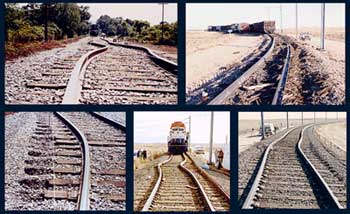
\includegraphics[scale=0.7]{pictures/Failure-theories/Rail_buckle}
    \caption{Train track buckling. (US Department of Transportation)}
  \end{figure}
\end{example}
\begin{solution}

  Buckling due to thermal load is a combination between two problems: buckling and thermal load. Assuming that rail buckling happens on a first mode ($n = 1$), we have that

  \begin{align*}
    P_{cr} &= \frac{ \pi^2 EI }{ L^2 } 
  \end{align*}

  Now we need to determine the change in temperature that will lead to that critical load. Let points A and B be the two ends of the rail. Following steps to solve a statically indeterminate problem (equilibrium equation, compabitility equation, and Hooke's law), we can write that:

  \begin{align*}
    F_A = F_B = F
  \end{align*}

  Since the two ends of the rail are supported, its length cannot change, i.e. the changes in length due to support force and thermal change must cancel out.

  \begin{align*}
    &\delta_{AB} = 0 \\
    &\delta_T + \delta_F = 0
  \end{align*}

  Applying Hooke's law and thermal elongation to the equation, we can solve for the support force $F$

  \begin{align*}
    &\alpha \Delta T L + \frac {FL}{AE} = 0 \\
    &F = -\alpha \Delta T A E
  \end{align*}

  Finally, we know that the support force $F$ must be equal to the critical load $P_{cr}$ to cause buckling. We must, however, flip the sign of $F$ because $F > 0$ is tensile load while $P_{cr}$ is always compressive.

  \begin{gather*}
    -F = P_{cr} \hfill \\
    \alpha \Delta T A E = \frac{ \pi^2 EI }{ L^2 } \hfill \\
    \begin{aligned}
      \Delta T &= \frac{ \pi^2 I }{ \alpha A L^2} = \frac{1}{\alpha} \left( \frac{ \pi r_g }{L} \right)^2 \\
      &= \frac{ \pi^2 (400 \times 10^{-8}) }{ (12 \times 10^{-6})(73 \times 10^{-4})(10^2)}\\
      &= 4.51^{\circ} \text{ C}
     \end{aligned}
  \end{gather*}

  As we can see it requires very slight temperature change to cause buckling. However, with a proper installation technique called \emph{rail stressing}, the rail is pre-stretched before installation. This technique preloads the rail in tension and thus it will be much less likely to buckle.
\end{solution}

\section*{Summary}

In this chapter, we study various ways engineering materials can fail. The first two, yield/fracture and fatigue are due to damage inflicted to the material by stress. Buckling, on the other hand, is due to the geometric instability of the structure brought upon by external compressive loads.

For yield and fracture, failure is due to static load. Yield occurs usually in ductile materials, while fracture occurs in brittle materials. The criteria introduced can be used to determine ‘equivalent’ stress to determine whether yield or fracture will occur in case of multiaxial stress.

Fatigue is due to repeated or periodic loading. The size of the load itself is not sufficiently large to cause yield or fracture to the material immediately, but after several cycles, the cumulative damage can cause failure. We have derived equations relative the stress amplitude to the number of cycles before failure, which also depends on material properties and whether the average stress is zero.

Buckling occurs because the internal bending moment in the beam is not enough to counter the external bending moment caused by the axial compressive load if a slight lateral perturbation occurs. The critical axial load depends on the dimensions of the body, material properties, and support conditions.

\section*{Exercises}

\begin{exercises}
  
  \exercise A plane stress element is under the following state of stress.  $\sigma_x = 150$ MPa, $\sigma_y = -200$ MPa , and $\tau_{xy} = 100$ MPa. The material has $S_y$ = 200 MPa, $S_{ut}$ = 250 MPa, and $S_{uc}$ = 300 MPa. Determine the safety factor under the following criteria.
  \begin{enumerate}
  \item MNST
  \item MSST
  \item MDET
  \item Modified Mohr-Coulomb theory
  \end{enumerate}

  \begin{figure}[H]
    \centering
    \begin{tikzpicture}
      \node [draw, fill=LightBlue, regular polygon, regular polygon sides=4, minimum width=2cm](A){};
      \draw [<-,very thick] (A.north) --++ (90:1) node[above]{$\sigma_y$ = -20 MPa};
      \draw [->,very thick] (A.east) --++ (0:1) node[right]{$\sigma_x$ = 150 MPa};
      \draw [->,very thick] (A.west) --++ (180:1);
      \draw [<-,very thick] (A.south) --++ (-90:1);
      \node at (A.north west) [yshift=2mm] (B){};
      \draw [-left to, very thick] (B) --++ (0:1.3);
      \node at (A.south east) [xshift=2mm] (C){};
      \draw [-right to, very thick] (C) --++ (90:1.3) node[above right]{$\tau_{xy}$ = 100 MPa};
      \node at (A.north west) [xshift=-2mm] (D){};
      \draw [-right to, very thick] (D) --++ (-90:1.3);
      \node at (A.south east) [yshift=-2mm] (E){};
      \draw [-left to, very thick] (E) --++ (180:1.3) ;
    \end{tikzpicture}
  \end{figure}
  
  \exercise A 2-m long, pinned-support prismatic steel ($E$ = 210 GPa) column is restrained in the middle. Its cross-sectional area is a circle with radius of 5 mm. Determine the safety factor of the column if it is compressed by the load of 7 MN.

  \begin{figure}[H]
    \centering
    \begin{tikzpicture}
      \node at (0,0) [anchor=south, draw, rectangle, minimum height=0.4cm, minimum width=8cm,fill=LightBlue](A){};
      \node at (A.west) [anchor=east, draw, regular polygon, regular polygon sides=3, minimum height=4mm, inner sep=0, fill=LightGrey, shape border rotate=30](C){};
      \node at (A.west) [draw, circle, inner sep=1.5, fill=LightGrey]{};
      \node at (A.east) [anchor=west, draw, regular polygon, regular polygon sides=3, minimum height=4mm, inner sep=0, fill=LightGrey, shape border rotate=-30](B){};
      \node at (A.east) [draw, circle, inner sep=1.5, fill=LightGrey]{};
      \node at (B.east) [anchor=west,rectangle, pattern=north east lines, minimum height=2cm, minimum width=0.5cm]{};
      \draw [<-, line width=2pt] (C.west) -- ++ (180:1) node[left]{$P$ = 7 MN};
      \node at (A.north) [anchor=south, draw, regular polygon, regular polygon sides=3, minimum height=4mm, inner sep=0, fill=LightGrey, shape border rotate=60]{};
      \node at (A.north) [draw, circle, inner sep=1.5, fill=LightGrey]{};
      \node at (A.south) [anchor=north, draw, regular polygon, regular polygon sides=3, minimum height=4mm, inner sep=0, fill=LightGrey, shape border rotate=0]{};
      \node at (A.south) [draw, circle, inner sep=1.5, fill=LightGrey]{};
      \node at (A.south west) [yshift=-0.8cm](D){};
      \node at (A.south east) [yshift=-0.8cm](E){};
      \draw [|<->|] (D) -- (E) node[midway, below]{2 m};
    \end{tikzpicture}
  \end{figure}
  
  \exercise A shaft made of AISI 1020 ($E$ = 210 GPa, $S_y$ = 400 MPa, and $S_{ut}$ = 600 MPa) is twisted back and forth by the torque of $T$ = [-200, 200] Nm. Size the proper shaft so that its safety factor is 3.

  \begin{figure}[H]
    \centering
    \begin{tikzpicture}
      \node at (0,0) [draw, cylinder, inner sep=5, minimum height=8cm, minimum width=1cm, fill=LightBlue](A){};
      \draw [->>, ultra thick] (A.east) ++ (180:5pt) --++(0:1) node[right]{$T$};
      \draw [->>, ultra thick] (A.west) --++(180:1) node[left]{$T$};
    \end{tikzpicture}
  \end{figure}

  \exercise You want to design a cylindrical beer can with 3 cm radius that contains a nice cold beer under 20 kPa pressure using the smallest possible thickness $t_1$. After you submitted the design to your manager, however, he told you to revise the design because when beer is shaken, it releases $\text{CO}_2$ that pressurizes the can to 60 kPa, using the smallest possible thickness $t_2$ but keeping the same 3 cm radius. If the aluminum used to manufacture the cans has a yield stress of 100 MPa, what is the difference in thickness between your second design and your first design $t_2 - t_1$? Note: use maximum distortion energy theory to determine failure.

    \begin{figure}[H]
    \centering
    \begin{tikzpicture}
      \node at (0,0) [draw, cylinder, inner sep=10, minimum height=4cm, minimum width=3cm, rotate=90, fill=LightBlue, fill opacity=0.5](E){};
      \node at (E.west) [draw, ellipse, dashed, minimum height=0.5cm, minimum width=2.8cm, yshift=10]{};
      \node at (5,0) [draw, circle, fill=LightBlue, inner sep=1cm](A){};
      \node at (5,0) [draw, circle, fill=White, inner sep=0.9cm](B){};
      \node at (A.west) [yshift=1.5cm](C){};
      \node at (A.east) [yshift=1.5cm](D){};
      \draw [|<->|] (C) -- (D) node[midway,above]{3 cm};
      \draw [|<-] (A.west) -- ++ (180:0.5) node[left]{$t$};
      \draw [|<-] (B.west) -- ++ (0:0.5);
    \end{tikzpicture}
  \end{figure}
  
\end{exercises}

%%%%%%%%%%%%%%%%%%%%%%%%%%%%%%%%%%%%%%%%%%%%%%%%%%%%%%%%%%%%%%%%%%%%%%%%%%%%%%%%%%%%%%%%%%%%%%%%%%%%%%%%%%%%%%%%%%%%%%%%%%%%%%%%%%%%%%%%%%%%%%%%%%%%%%%%%%%%%%%%%%%%%%%%%%%%%%%%%%%%%%%%%%%%%%%%%%%%%%%%%%%%%%%%%%%%%%%%%%%%%%%%%

\part{The Components}

%%%%%%%%%%%%%%%%%%%%%%%%%%%%%%%%%%%%%%%%%%%%%%%%%%%%%%%%%%%%%%%%%%%%%%%%%%%%%%%%%%%%%%%%%%%%%%%%%%%%%%%%%%%%%%%%%%%%%%%%%%%%%%%%%%%%%%%%%%%%%%%%%%%%%%%%%%%%%%%%%%%%%%%%%%%%%%%%%%%%%%%%%%%%%%%%%%%%%%%%%%%%%%%%%%%%%%%%%%%%%%%%%

\chapter{Design of Simple Load Bearing Elements}

Load bearing elements are designed to support forces, moments, or torques and transfer them to their intended destination. A beam typically supports a vertical load using its bending stiffness and transfer the load to a wall or column. A column takes a vertical load and transmit it to the foundation—as in a building or a structure. The main purpose of a shaft is to transfer torque about its longitudinal axis to a support or a rotational member.

The goal of this chapter is to develop the fundamental concepts involved in designing load bearing elements to properly resist their respective loads under given constraints.

\section{Basis for Beam Design}

Beams are often designed based on their strength so that they can resist internal bending moment and shear force developed along their length. Though it is arguable that some beams are also subjected to axial load in operation, the resultant stress from such loads are typically negligible compared to those from bending moment and shear force. It is also assumed that the beam material is homogeneous and has linear elastic behavior. We have discussed the formulas that establish the relationship between bending moment and normal stress and shear force and shear stress in \cref{section: bending}.

Although beams are mostly design for strength, they must be braced along their sides in certain cases to provide additional stability and prevent buckling. Furthermore, in some cases beams must be designed to resist a limited amount of deflection, such as when they support ceilings made of brittle materials. Methods for finding deflections are discussed in \cref{subsection: beam deflection}, and beam buckling is discussed in details in \cref{section: buckling}.

The beam bending and shear stress formulas are employed to for beam design; we will discuss the resultant stress of a cantilever beam when these two formulas are applied at various point along the length, assuming that the beam has a rectangular cross section and supports a load P at the free end.

In general, shear stress distribution in a beam takes a parabolic shape, while normal stress distribution takes a linear shape, shown in \cref{fig: stress in beam}. Notice that the top and bottom parts of the beam only take normal stress, while the middle part only takes shear stress. Any other region of the beam takes a combination of normal and shear stresses.

\begin{figure}[h]
  \centering
  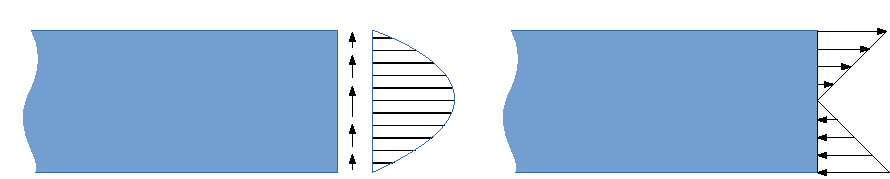
\includegraphics[scale=1]{pictures/Simple-load-bearing/stress-in-beam}
  \caption{Shear and normal stress distributions in a cantilever beam.}
  \label{fig: stress in beam}
\end{figure}

At each point, the state of stress can be transformed into principal stresses. The results are shown in \cref{fig: stress traject in beam}. Notice that on the right column, the element undergoes a counterclockwise rotation, from $0^{\circ}$ at the top, to $45^{\circ}$ in the middle, to $90^{\circ}$ at the bottom.

\begin{figure}[h]
  \centering
  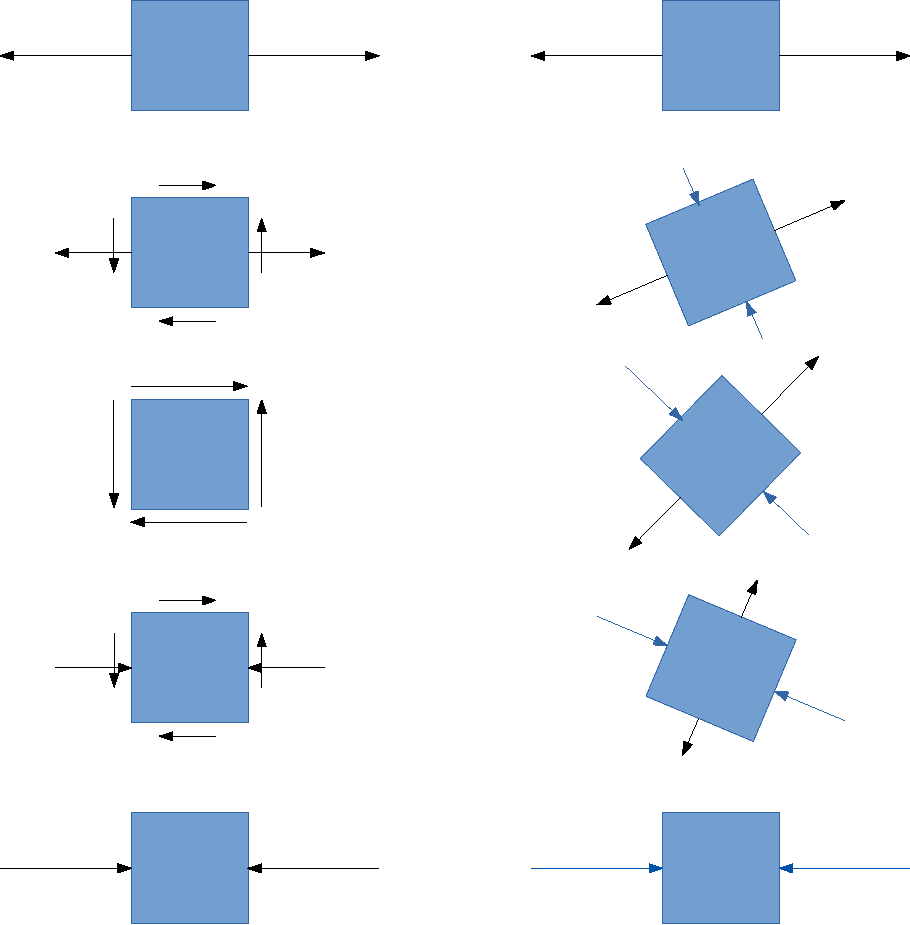
\includegraphics[scale=.6]{pictures/Simple-load-bearing/stress-traject-beam}
  \caption{State of stress and principal stresses of a cantilever beam throughout its thickness}
  \label{fig: stress traject in beam}
\end{figure}

If this analysis is expanded to other vertical cross sections throughout the length of the beam, the results can be represented by sets of curves called stress trajectories. Each of these lines represents the direction of a principal stress having a constant magnitude. Some of these trajectories are shown in Figure 5.3. In this figure, the solid lines represent the direction of the tensile principal stresses and the dashed lines represent the direction of the compressive principal stresses. The lines intersect the neutral axis at $45^{\circ}$ and the solid and dashed lines intersect at $90^{\circ}$ because principal stresses are always $90^{\circ}$ apart. Knowing these trajectories can help engineers determine where to reinforce a beam especially if the beam is made of brittle material so that it will not crack or become unstable.

\section{Prismatic Beam Design}

Most beams are made of ductile materials. When this is the case, it is generally unnecessary to plot stress trajectories. It is typically sufficient to make sure that the bending and shear stresses in the beam do not exceed allowable values. In most cases, the suspended section of the beam will be relatively long, so that the internal bending moments are large. With large bending moments, the first design concern is the normal bending stress, then shear stress. To control the normal stress, the beam must have sufficient section modulus. Following \cref{eqn: section modulus}, we have that the required section modulus of a beam with maximum bending moment $M_{\max}$ and allowable stress $\sigma_{allow}$ is

\begin{equation} \label{eqn: beam required section}
  S_{req} = \frac{M_{\max}}{\sigma_{allow}}
\end{equation}

It is important to note that the beam is assumed to be light so that its weight does not contribute significantly to the bending moment. If we do not make such assumption, the actual section modulus should be slightly larger than $S_{req}$. Once the section modulus is known, if the beam has a simple cross section like a square, a rectangle, or a circle, then its dimensions can be determined promptly since $S = I/c$. However, if the section is a complex shape or made up of several elements, there may be an infinite number of combinations that satisfy the value of $S_{req}$. In reality, engineers choose a particular beam meeting the section modulus requirement from a handbook or catalog that lists available standard shapes from manufacturers. If deflection is not a concern, then the beam with the smallest cross-sectional area (which is also the lightest and most economical) is chosen. If there is a constrain on deflection $\delta_{allow}$, however, a generalized beam deflection equation can be used to determine the required moment of inertia $I_{req}$.

\begin{equation}
  I_{req} = k \frac{FL^3}{E \delta_{allow}}
\end{equation}

where the constant $k$ depends on the location of load $F$ along the beam and support conditions.
  
Once the beam has been selected, engineers can use the shear-stress formula $\tau_{allow} = VQ/Ib$ to check for excessive shear stress. Typically this is not a problem. However, in cases where the beam is short, thick, and supporting a large concentrated load, this shear stress limitation may dictate the size of the beam. This is especially important for wooden beams as they are prone to failure along the grain due to shear.

\section{Fabricated Beams}

Since beams are often made of steel or wood, we will discuss some of the tabulated properties of beams made from these materials.

\subsection{Steel sections}
Most manufactured steel beams are made by the process of rolling hot steel into
a desired shape of cross section. These rolled shapes have properties that have
been tabulated in the American Institute of Steel Construction (AISC) manual.
The properties of wide-flange (W shape), channel (C shape), and angle members
are listed in \cref{appendix: structural steel properties}. For example, a W610
$\times$ 155 indicates a wide-flanged cross section having a depth of 610 mm and
a weight of 155 kg/m. For any given section, the weight per length, dimensions,
cross-sectional area, moment of inertia, section modulus, and the radius of
gyration are reported. Notice that in structural steel sections, the tables will
report the properties according to its neutral axis. We must use the beam
along the axis which can resist the highest stress and deflection.

\begin{figure}
  \centering
  \begin{tikzpicture}
    \draw [fill=lightblue] (0,0) ++ (0:0.2) --++ (90:1) --++ (10:1) --++ (90:0.2) --++ (180:2.2) --++ (-90:0.2) --++ (-10:1) --++ (-90:2) --++ (-170:1) --++ (-90:0.2) --++ (0:2.2) node[midway, below]{S shape} --++ (90:0.2) --++ (170:1) --cycle;
    %\draw [dashed] (0.1,-2) node[below]{2}--++ (90:4) node[above]{2};
    %\draw [dashed] (-1.5,0) node[left]{1} --++ (0:3) node[right]{1};
  \end{tikzpicture} 
  \hspace{1cm}
  \begin{tikzpicture}
    \draw [fill=lightblue] (0,0) ++ (0:0.2) --++ (90:1.1) --++ (0:1) --++ (90:0.3) --++ (180:2.2) --++ (-90:0.3) --++ (0:1) --++ (-90:2.1) --++ (180:1) --++ (-90:0.3) --++ (0:2.2) node[midway, below]{W shape} --++ (90:0.3) --++ (180:1) --cycle;
    % \draw [dashed] (0.1,-2) node[below]{2}--++ (90:4) node[above]{2};
    % \draw [dashed] (-1.5,0) node[left]{1} --++ (0:3) node[right]{1};
  \end{tikzpicture}
   \hspace{1cm}
  \begin{tikzpicture}
    \draw [fill=lightblue] (0,0) --++ (180:1) node[midway, below]{C shape} --++ (90:2.7) --++ (0:1) --++ (-90:0.3) --++ (180:0.7) --++ (-90:2.1) --++ (0:0.7) -- cycle;
  \end{tikzpicture}
  \hspace{1cm}
  \begin{tikzpicture}
    \draw [fill=lightblue] (0,0) --++ (0:2.7) node[midway, below]{L shape} --++ (90:0.3) --++ (180:2.4) --++ (90:2.4) --++ (180:0.3) -- cycle;
  \end{tikzpicture}
  \caption{Structural steel sections}
\end{figure}

To choose a proper steel section, we follow the same process as any prismatic
beam design. Determine the required section modulus $S_{req}$ and moment of
inertia $I_{req}$ from the stress and deflection requirement, respectively.
Subsequently, the optimal section can be selected on minimum weight or minimum cost criterion.

\begin{example}
  A gantry crane with 3-m span has a maximum load capacity of 3 ton. Determine a proper structural steel (S shape) so that the safety factor is 3 and the maximum deflection does not exceed 1 cm.

  \begin{figure}[H]
    \centering
    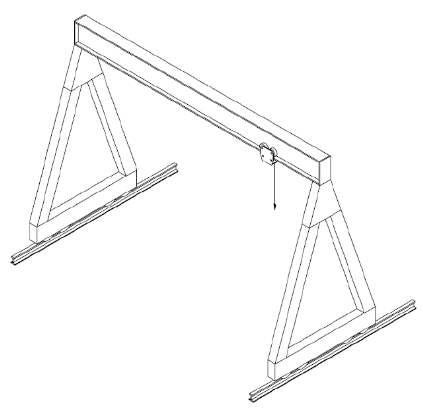
\includegraphics[scale=0.55]{pictures/Simple-load-bearing/gantry-crane}
  \end{figure}
\end{example}
\begin{solution}
  In this problem, first of all, we must make sure that the designed beam does not fail under the 3-ton load regardless of the weight position on the crane. With the beam supported on both ends, the maximum bending moment occur when the load is hoisted from the middle. The corresponding bending moment is $M = FL / 4$ and the required section modulus $S_{req}$ is

  \begin{align*}
    S_{req} &= \frac{N_s M}{S_y} \\
            &= \frac{(3)(3000)(10)(3)/4}{250 \times 10^6} \\
            &= 2.7 \times 10^{-4} \text{ m}^3 = 2.7 \times 10^5 \text{ mm}^3
  \end{align*}

  Refering to \cref{table: s-shaped sections}, the proper section is S250 $\times$ 37.8.

  The problem also specified the maximum deflection, which also occurs in the middle of the beam when there is a midpoint load. The expression for the deflection of a beam with simple supports is

  \begin{align*}
    \delta &= \frac{FL^3}{48EI_{req}} \\
    I_{req} &= \frac{30000(3^3)}{48(210 \times 10^9)(0.01)} \\
           &= 8.04 \times 10^{-6} \text{ m}^4 = 8.04 \times 10^6 \text{ mm}^4
  \end{align*}

  Using the same table, the proper section is S150 $\times$ 18.6.

  Finally, we see that the $S_{req}$ requires a larger section, and should be our designed beam.
\end{solution}

\subsection{Wood sections}

Most wooden beams have rectangular cross sections because they are easy to manufacture and handle. Manuals list the dimensions of lumber often used in beam design. Lumber is identified by its nominal dimensions, for example 2 $\times$ 4. However, its actual dimensions are smaller (1.5 $\times$ 3.5) because lumber must be further processed to obtain a smooth surface. The actual dimensions, of course, must be used when calculating stresses in a wooden beam.

\subsection{Built-up sections}

A built-up section is made from two or more parts joined together. Since the ability of a beam to resist moment depends on its section modulus, which in turn depends on its moment of inertia, beam material should be placed as far away as possible from its neutral axis. This is what makes wide-flanged beam so effective in resisting bending moment with minimal weight.

For very large loads, however, there may not be a beam with a sufficiently large section modulus. Engineers often “build up” a beam made of plates and angles. A beam with deep I-shaped cross section made from built-up plates and angles are called a plate girder where angles are either bolted or welded to plates forming I-shape, illustrated in \cref{fig: steel fabricated beam}.

\begin{figure}[h]
  \centering
  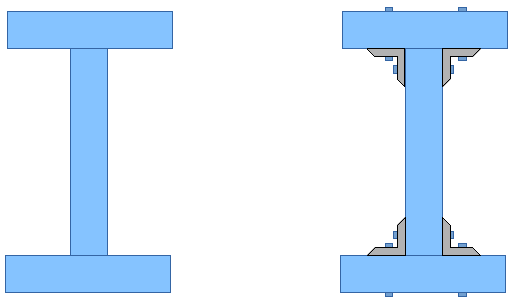
\includegraphics[scale=0.8]{pictures/Simple-load-bearing/steel-fab-beams}
  \caption{Welded and bolted steel girders each made from 3 plates and 4 angles }
  \label{fig: steel fabricated beam}
\end{figure}

Wooden beams can also be built-up, usually form a box beam section. For larger spans, glulam beams, made from glue-laminating multiple boards together to form a thick rectangular section, can be used.

Just as in the case of rolled steel or wooden sections made from a single piece, built-up beams must be checked so that their bending and shear stresses do not exceed the allowable values of any of the parts. Additionally, the stress of the fasteners (welds, bolts, or glue) must also be checked to prevent the beams from coming apart.

\section{Fully Stressed Beams}

Since the moment in a beam generally varies along its length, prismatic beams are not usually the most efficient choice for resisting moment since it is never fully stressed where the moment is smaller than the maximum moment in the beam. In order to reduce weight, engineers sometimes choose a variable cross-sectioned beam in such a way that at each cross section along the beam, the bending stress reaches its maximum allowable value. Beams having a variable cross section are called nonprismatic beams. They are often used in machines since they can be formed by casting. They can also be built-up using plates or angles to reinforce the location where the bending moment or shear force is expected to be the highest.

The stress analysis of a nonprismatic beam is typically very complicated. In most cases, analyses are carried out with a computer. The results obtained, however, does indicate that the assumptions used in the flexure formula are approximately correct for predicting bending stresses in nonprismatic beams provided that the rate of change of the cross section is not too severe. On the other hand, the shear formula cannot be used for nonprismatic beams since the results can be very misleading.

Though caution is advised when designing beams using the flexure formula, we can see that by applying \cref{eqn: flexure formula} the general shape of the beam can be determined. The only difference is that $S_{req}$ is now a function of the position along the length of the beam. A beam designed this way is called a fully stressed beam. It is important to note that only the bending stress is considered here, and shear stress must be carefully checked in its final shape, especially at the locations of concentrated loads.

\begin{example}

  Determine the cross section of a fully stressed, rectangular cross-sectioned cantilever beam with a downward load at the free end.
\end{example}

\begin{solution}
  For a cantilever beam of length $L$ that is fixed on the left end, the bending moment as a function of position along the length is

  \[M(x) = F(x-L)\]

  Assume that the base and thickness of the beam as functions of length are $b(x)$ and $h(x)$, respectively. We can rewrite \cref{eqn: beam required section} as

  \[{\renewcommand{\arraystretch}{2.5}
  \begin{array}{l}
    S_{req} = \dfrac{M(x)}{\sigma_{allow}} = \dfrac{F(x-L)}{\sigma_{allow}} \\
    \dfrac{b(x)h(x)^2}{6} = \dfrac{F(x-L)}{\sigma_{allow}} \\
    b(x)h(x)^2 = \dfrac{6F(x-L)}{\sigma_{allow}}
  \end{array}}\]

This function $bh^2 = 6F(x-L)/\sigma_{allow}$ determines the general cross-sectional shape along the beam length. Being a two-variable function, it does not provide us with the sense of what that shape is. We can, however, set one variable as a constant and obtain the shape described by the other.

First, let us set $h$ as a constant, the required base length $b$ becomes

\[b(x) = \dfrac{6F(x-L)}{h^2 \sigma_{allow}}\]

With all other variables set to constants, $b(x)$ is simply a linear function along the beam length, i.e. the beam forms a wedge.

\begin{figure}[H]
  \centering
  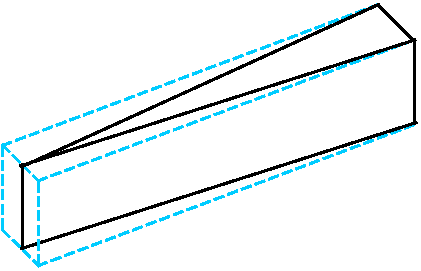
\includegraphics[scale=0.7]{pictures/Simple-load-bearing/fully-stressed-wedge}
\end{figure}

If instead, $b$ is set as a constant, the required thickness of the beam is

\[h(x) = \sqrt{\dfrac{6F(x-L)}{b \sigma_{allow}}}\]

$h$ in this case is a parabola.

\begin{figure}[H]
  \centering
  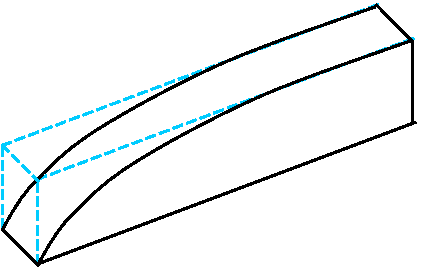
\includegraphics[scale=0.7]{pictures/Simple-load-bearing/fully-stressed-parabola}
\end{figure}
\end{solution}
\section{Shaft Design}

Shafts with circular cross sections are the staple of machine design. They are used to transfer torque and set alignment to rotational components. As such, they are usually subjected to cyclic loading and fatigue stress, caused by the torsional and bending loads they must transfer or resist. In addition to these loads, various components and features such as keys, couplings, or sudden changes in cross-sectional area of the shaft can cause stress concentrations. To properly design a shaft, all of these considerations must be taken into account.

In this section, we will discuss the important aspects of the design of shafts required for power transmission. These shafts are subjected to loads transferred from attached pulleys or gears. Since the loads applied to the shaft can come from many angles, the internal bending and torsional moments at any cross section can be determined by breaking for loads down into their Cartesian components. With that, equilibrium equations can be written from the loads in each plane, and the resultant moment can then be determined using vector addition. In addition, segments of the shaft can be subjected to different torques, which can be addressed by constructing a \emph{torque diagram}. Also, if there exist any axial loading on the shaft, either due to external load or due to attached angled worms or gears, the resultant axial stress must be incorporated in the analysis as well

Once internal bending moment, torque, and axial load along the length of the shaft have been determined, the next task is to determine the critical point in the shaft—the location where the combination of moment and torque causes the worst stress situation. Furthermore, external forces can cause shear stresses from $\tau = VQ/Ib$. In most cases, however, these shear stresses are small compared to the stresses due to bending and torsional moments. In general, the critical point is subjected to plane stress so that

\begin{figure}
  \centering
  \begin{tikzpicture}[>=latex]
    \node (0,0) [draw, cylinder, fill=lightblue, minimum height=6cm, minimum width=1cm, inner sep=4] (F) {};
    \draw [->] (F.west) ++ (90:0.1)--++ (180:1) node[above left]{$F$};
    \draw [->] (F.east) ++ (90:0.1) --++ (0:1) node[above right]{$F$};
    \draw [->>, very thick] (F.west) --++ (180:2) node[left]{$T$};
    \draw [->>, very thick] (F.east) --++ (0:2) node[right]{$T$};
    \draw [->] (F.west) ++ (90:1) node[right]{$M$} arc (135:225:1.5);
    \draw [->] (F.east) ++ (90:1) node[left]{$M$} arc (45:-45:1.5);

    \node at (F.north) [anchor=north, draw, rectangle, minimum height=1mm, minimum width=2mm, inner sep=0pt]{};
    \draw [<-] (F.north) --++ (60:0.5) node[above]{Critical point};

    % critical point element
    \node at (0,-3) [draw, fill=lightblue, regular polygon, regular polygon sides=4, minimum width=2cm](A){};
    \draw [->,very thick] (A.east) --++ (0:1) node[right]{$\sigma = \dfrac{Mr}{I} + \dfrac{F}{A}$};
    \draw [->,very thick] (A.west) --++ (180:1);
    \node at (A.north west) [yshift=2mm] (B){};
    \draw [-left to, very thick] (B) --++ (0:1.3);
    \node at (A.south east) [xshift=2mm] (C){};
    \draw [-right to, very thick] (C) --++ (90:1.3) node[above right]{$\tau = \dfrac{Tr}{J}$};
    \node at (A.north west) [xshift=-2mm] (D){};
    \draw [-right to, very thick] (D) --++ (-90:1.3);
    \node at (A.south east) [yshift=-2mm] (E){};
    \draw [-left to, very thick] (E) --++ (180:1.3) ;
  \end{tikzpicture}
  \caption{State of stress at the critical point of a shaft with multiple loadings.}
\end{figure}

\[\sigma  = \frac{Mr}{I} + \frac{F}{A} \hspace{1cm} \tau  = \frac{Tr}{J}\]

If the allowable normal or shear stress for the material is known, we can apply a corresponding theory of failure to determine the proper size of the shaft. For example, if the shaft is ductile we can apply the maximum shear stress theory, which requires that the maximum allowable shear stress be equal to the maximum shear stress in the shaft. Using stress transformation, we have that

\[\begin{gathered}
    \tau_{allow} = \tau_{\max} = \sqrt {\left( \frac{\sigma}{2} \right)^2 + {\tau ^2}}  \\ 
    = \sqrt{ \left( \frac{Mr}{2I} + \frac{F}{2A} \right)^2 + \left( \frac{Tr}{J} \right)^2}  \\ 
  \end{gathered} \]

Since $I = \pi r^4/4$ and $J = \pi r^4/2$, the above equation becomes

\begin{equation}
  \begin{gathered}
    \tau_{allow} = \sqrt{ \left( \frac{2M}{\pi r^3} + \frac{F}{2 \pi r^2} \right)^2 + \left( \frac{2T}{\pi r^3} \right)^2 } \\
    r = \left( \frac{1}{2 \pi \tau _{allow}} \sqrt {(4M + Fr)^2 + 16T^2 } \right)^{\frac{1}{3}}
  \end{gathered}
\end{equation}

If the shaft design calls for a safety factor $N_s$, then the required radius is

\begin{gather*}
  r = \left( \frac{N_s}{2 \pi \tau _{allow}} \sqrt {(4M + Fr)^2 + 16T^2} \right)^{\frac{1}{3}}
\end{gather*}

The above equation cannot be analytically solve, except when $F=0$, in which case

\begin{equation} \label{eqn: shaft radius without axial}
  r = \left( \frac{2 N_s}{\pi \tau_{allow}}\sqrt {M^2 + T^2} \right)^{\frac{1}{3}} 
\end{equation}

Note that the application of any other theories of failure or safety factor other than one will result in a different value for the radius $r$. In more complex scenarios, it may be necessary to apply this methodology to all possible candidates of a critical point to determine the largest required radius.

\begin{example} A 1-m long shaft is fitted with a pully and timing belt. The tensions on the slack and tight sides are 2000 N and 500 N respectively. The pulley radius is 5 cm. Size the proper shaft size so that it has a safety factor of 2.5. The shaft is made of AISI1023 with $S_y$ = 400 MPa.

  \begin{figure}[H]
    \centering
    \begin{tikzpicture}[>=latex]
      % left support
      \node at (0,0) [ellipse, draw, fill=LightGrey, rotate=-30, minimum height=2cm, minimum width=0.8cm](A){};
      % left shaft
      \node [anchor=west,cylinder, fill=LightBlue, draw, rotate=-30, minimum height=3.5cm, minimum width=1cm] (c){};
      % pulley
      \node at (c.east) [ellipse, draw, fill=LightGrey, rotate=-30, minimum height=3cm, minimum width=1.2cm](b){};
      % right shaft
      \node at (b) [anchor=west,cylinder, fill=LightBlue, draw, rotate=-30, minimum height=3.5cm, minimum width=1cm](d){};
      % right support
      \node at (d.east) [ellipse, draw, fill=LightGrey, rotate=-30, minimum height=2cm, minimum width=0.8cm](B){};
      \draw [->, very thick] (b.north west) -- ++(-150:4) node[below left]{2000 N};
      \draw [->, very thick] (b.south east) -- ++(-150:4) node[below left]{500 N};
      % pulley radius dimensioning
      \draw [dashed] (b.center) --++ (-150:2);
      \draw [<->] (b.center) ++ (-150:1.5) --++ (90:1.05) node[midway, left, rotate=30]{5 cm};
      % shaft length dimensioning
      \draw [|<->|] (c.west) ++ (60:1.5) --++ (-30:3.5) node[midway, above, rotate=-30]{30 cm};
      \draw [|<->|] (d.west) ++ (60:1.5) --++ (-30:3.5) node[midway, above, rotate=-30]{30 cm};
    \end{tikzpicture}
  \end{figure}
  
\end{example}

\begin{solution}
  Upon inspection, this power transmission mechanism does not have any helical or bevel gear that can exert axial load, so the shaft is subjected to only bending and torsion. What we need to do here is to determine the critical point location and corresponding stresses which should lead us to the required shaft radius.

  The shaft is supported by bearings on both sides, though it did not make any mention about whether it is a fixed or simple support. Applied torque in this problem does not depend on the type of support, while bending moment may. However, when the applied load is in the middle of the shaft like here, the type of support does not impact the bending moment either.

  We have seen bending problems with midpoint loads many times before, so we know that the critical point is in the middle at the top of bottom surface of the shaft. Shear stress from torsion is uniform on the surface. The state of stress at the critical point reduces to

  $$ \sigma = \frac{Mr}{I} $$
  $$ \tau = \frac{Tr}{J} $$

  in which case, the required shaft radius from \cref{eqn: shaft radius without axial} is

  \begin{align*}
    r &= \left( \frac{2 N_s}{\pi \tau _{allow}}\sqrt {M^2 +T^2}  \right)^{\frac{1}{3}} \\
      &= \left( \frac{2 \times 2.5}{\pi (400 \times 10^6 /2 )}\sqrt {[(2000+500)(0.6/4)]^2 +[(2000-500)(0.05)]^2}  \right)^{\frac{1}{3}} \\
      &= 1.51 \times 10^{-2} \text{ m} = 1.51 \text{ cm}
  \end{align*}

  Note that $\tau_{allow}$ is derived from maximum shear stress theory, for which $\tau_{allow} = S_y/2$.
\end{solution}

\section{Column Design}

In the previous sections, we discussed the design of members based on strength and deflection by assuming that they are always in equilibrium and stable. However, columns under axial compression can be subjected to large enough load to cause it to buckle. This can often lead to a sudden and dramatic failure of a structure or mechanism. Hence, special attention must be given to the design of columns so that they can support their intended loads without buckling.

\subsection{Design of simple columns}

Simple columns refer to prismatic columns with homogeneous materials and ideal supports. The governing equations of these columns have already been derived and discussed in details in \cref{section: buckling}. Employing \cref{eqn: Euler's formula}, we have that the critical load for a column is

\[P_{cr} = \frac{\pi ^2EI}{(KL)^2}\]

where $K$ is a constant based on the column supports. For a given column length $L$ and a given column material, its moment of inertia $I$ is

\begin{equation}
  I_{req} = \frac{P_{cr}(KL)^2}{\pi ^2E}
\end{equation}

The cross section dimensions can then be easily determined once its shape is selected. For example, considering columns with circular cross sections. The required radius is

\begin{equation}
  r_{req} = \left( \frac{4I_{req}}{\pi } \right)^{\frac{1}{4}}
\end{equation}

Similar derivations can be used to compute dimensions for columns with square or rectangular (with known width-to-height ratio) cross sections.

\subsection{Design of columns for concentric loading} \label{subsection: column concentric loading}

The theory presented in the previous section applies to columns that are perfectly straight, made of homogeneous material, and originally stress free. In reality, none of these conditions can practically be met. Also, column supports are hardly ideal, and load applications are even less so. To compensate for these imperfections, many design codes require the use of formulas based on empirical data. By performing large numbers of experiments, the results can be plotted and design formulas can be determined using curve fitting.

In order to account for the behavior of columns with different lengths, design codes usually give formulas that will best fit the data within the short, medium, and long column range. Each formula will only apply to a certain range of slenderness ratio. Examples of design formulas for steel, aluminum, and wood columns that are currently in use will be discussed. It is important to note that these formulas should not be used for the design of actual columns unless the codes from which they are referenced is used.

\subsubsection{Steel columns}

Columns made of structural steel can be designed on the basis of formulas proposed by the Structural Stability Research Council (SSRC). Safety factors have been applied to these formulas and adopted as specifications for building construction by the American Institute of Steel Construction (AISC). These specifications give two formulas for column design, which give the maximum allowable stress in the column for a specific range of slenderness ratio.

For long columns, the Euler’s formula--\cref{eqn: Euler's formula}--is proposed

\[\sigma_{\max} = \frac{\pi^2E}{\lambda^2}\]

where $\lambda = KL/r_g$ is the slenderness ratio and $r_g$ is the radius of gyration of the column cross section. The application of this formula requires the safety factor of 23/12 = 1.92 so that

\[\sigma_{allow} = \frac{12\pi^2E}{23\lambda^2} \hspace{1cm} \lambda_c \leqslant \lambda \leqslant 200\]

This equation is applicable for the slenderness ratio between 200 and $\lambda_c$. This latter value is there to prevent the material reaching inelastic region. Experiments show that compressive residual stress can exist in rolled steel sections for an upward amount of one-half of the yield strength. Therefore, if the compressive stress in the material is more than one-half the yield strength, the material will be in the inelastic region and the formulas no longer apply. The value of $\lambda_c$ is therefore

\begin{gather*}
  \frac{S_y}{2} = \frac{\pi ^2E}{\lambda_c^2} \hfill \\
  \lambda_c = \sqrt {\frac{2\pi^2E}{S_y}}  \hfill 
\end{gather*}

Columns having slenderness ratio less than $\lambda_c$ are designed on the basis of an empirical formula that has the form

$$ \sigma _{\max} = \left[ 1 - \frac{\lambda^2}{2\lambda_c^2} \right]S_y $$

There is more uncertainty for longer columns, and the safety factor must reflect this. It takes the form

$$ N_s = \frac{5}{3} + \frac{3\lambda}{8\lambda_c} - \frac{\lambda^3}{8\lambda_c^3} $$

Note that the safety factor is 5/3 = 1.67 when $\lambda$ = 0 and increases to 23/12 = 1.92 when $\lambda = \lambda_c$. Therefore, for design purpose

\begin{equation}
  \sigma_{allow} = \frac{\sigma_{\max}}{N_s} = \frac{\left[ 1 - \dfrac{\lambda^2}{2\lambda_c^2} \right] S_y }{\dfrac{5}{3} + \dfrac{ 3\lambda }{8\lambda_c} - \dfrac{\lambda^3}{8\lambda_c^3}}
\end{equation}

\begin{figure}[h]
  \centering
  \begin{tikzpicture}
    \begin{axis}[
      width=0.9\textwidth,
      height=.6\textwidth,
      xmin=0,xmax=200,
      ymin=0,ymax=1,
      axis background/.style={fill=SkyBlue!50},
      ytick distance=0.2,
      xticklabels={,,},
      xlabel={Slenderness Ratio $\lambda$},
      ylabel={$\dfrac{\sigma_{allow}}{S_y}$},
      ylabel style={rotate=-90},
      cycle list name=exotic,
      samples=100,
      no markers,
      grid=both,
      every axis plot/.append style={thick},
      ]
      \addplot [domain=0:100, DarkBlue]{(1-(x^2)/(2*100^2))/(5/3+3*x/(8*100)-x^3/(8*100^3))} node[midway, below left]{short column};
      \addplot [domain=100:200, DarkRed]{12/23*100^2/(2*x^2)} node[midway, above right]{long column};
      \addplot [domain=51:100, DarkGrey!20!Black, dashed] {12/23*100^2/(2*x^2)} node[near start, above right]{theory};
    \end{axis}
    \draw [dashed, Red] (6.3,0) --++ (90:8) node[at start, below]{$\lambda_c$};
  \end{tikzpicture}
  \caption{Ratio of designed allowable stress and yield strength as a function slenderness ratio of steel columns}
  \label{fig: steel column}
\end{figure}

\begin{example}
  Determine a proper cross section of a structural wide-flange steel beam (W-shape) for a gantry crane. The column is to take a compressive load of 50000 N and is to be 3 m tall. The safety factor of the column is 2. Consider the top part free and the bottom part fixed. Use these methods to determine the proper cross-sectional moment of inertia.
  \begin{enumerate}
  \item Ideal column assumption.
  \item AISC equation.
  \end{enumerate}
  Compare and discuss the results.
\end{example}
\begin{solution}
  For relatively long and slender columns, the only concern about choosing a proper cross-section is preventing buckling. For a fixed-free column, the effective length factor $K = 2$. In that case, we need to determine the minimum required moment of inertia $I_{req}$.

  Using ideal column assumptions, the critical load of a column is

  \begin{align*}
    P_{cr} &= \frac{\pi^2 EI}{4L^2}
  \end{align*}

  Incorporating safety factor, we can determine $I_{req}$ as
  
  \begin{align*}
    N_s &= \frac{P_{cr}}{P} \\
    I &= I_{req} = \frac{4 N_s P L^2}{\pi^2 E} \\
        &= \frac{4(2)(50000)(3^2)}{\pi^2 (210 \times 10^9)} \\
        &= 3.47 \times 10^{-6} \text{ m}^4
  \end{align*}

  Refering to the catalog for W-shape steel, the proper section is W360 $\times$ 39.

  Now, using the AISC equation, there is no analytical relationship for us to solve for the required $I$ or $r_g$. Instead, we must use the equation to calculate allowable load on each cross section. The generated allowable load data table is
  
  \begin{tabular}{ L{2.5cm} C{2cm} C{2cm} C{2cm} C{2cm} C{2cm}}
    \toprule
    W section & $r_g$ (mm) & $A$ (mm$^2$) & Slenderness Ratio & $\sigma_{allow}$ (MPa) & $P_{allow}$ (kN) \\
    \midrule
    W360 $\times$ 39 & 27.5 & 4960 & 218 & -63  & -314 \\
    W360 $\times$ 45 & 37.8 & 5710 & 159 & 32   & 183 \\
    W200 $\times$ 36 & 40.9 & 4570 & 147 & 46   & 211 \\
    W150 $\times$ 22 & 36.8 & 2860 & 163 & 26.6 & 76 \\
    \bottomrule
  \end{tabular}
  
  At first, we find that our original choice W360 $\times$ 39 does not have the proper slenderness ratio (218 was higher than 200). So we pick a next larger one, W360 $\times$ 45, but find that it can support much larger load than required. Subsequently, by process of elimination, we find the lightest section that still support sufficient compressive load is the W150 $\times$ 22.
  
\end{solution}

\subsubsection{Aluminum columns}

Column design for structural aluminum is specified by the Aluminum Association using three equations, each applicable to a specific range of slenderness ratios. Since several types of aluminum alloy exist, there is a unique set of formulas for each type. For a common alloy (2014-T6) used in building construction, the formulas are

\begin{equation}
  \sigma_{allow} = \left\{
    \begin{array}{lcc}
      1.93 \times 10^8 &&  0 \leqslant \lambda \leqslant 12 \\[20pt] 
      2.12 \times 10^8 - 1.59 \times 10^6 \lambda && 12 \leqslant \lambda \leqslant 55 \\[20pt]
      \dfrac{3.72 \times 10^{11}}{ \lambda^2 } && 55 \leqslant \lambda 
    \end{array} \right.
\end{equation}

Again, in these design equations, $\lambda = KL/r_g$. Notice that the first two parts are linear, used to model the effects of short and medium columns. The third has the same form as the Euler formula and is used for long columns.

\begin{figure}[h]
  \centering
  \begin{tikzpicture}
    \begin{axis}[
      width=0.9\textwidth,
      height=.6\textwidth,
      xmin=0,xmax=100,
      xlabel={$\lambda$},
      ylabel={$\dfrac{\sigma_{allow}}{S_{comp}}$},
      ylabel style={rotate=-90},
      cycle list name=exotic,
      samples=100,
      grid=both,
      axis background/.style={fill=SkyBlue!50},
      no markers,
      every axis plot/.append style={thick},
      ]
      \addplot [domain=0:12, DarkBlue]{1} node[midway, below]{short};
      \addplot [domain=12:55, DarkRed]{(2.12*10^8-1.59*10^6*x)/(1.93*10^8)} node[midway, above right]{medium};
      \addplot [domain=55:100, DarkGrey!20!Black] {1928/x^2} node[midway, above right]{long};
    \end{axis}
  \end{tikzpicture}
  \caption{Ratio of designed allowable stress to compressive strength for aluminum columns of various slenderness ratio}
  \label{fig: aluminum column}
\end{figure}
\subsubsection{Timber Columns}

Columns used in timber construction are designed based on formulas published by the National forest Products Association (NFPA) or the American Institute of Timber Construction (AITC). For example, the NFPA formulas for the allowable in short, intermediate, and long columns have a rectangular cross section of dimensions $b$ and $h$, where $h$ is the smallest dimension of the cross section, are

\begin{equation}
  \sigma_{allow} = \left\{
    \begin{array}{l c}
      8.27 \times 10^6 & 0 \leqslant \lambda \leqslant 11 \\ 
      8.27 \times 10^6\left[ 1 - \dfrac{1}{3} \left( \dfrac{\lambda}{26} \right)^2 \right] & 11 \leqslant \lambda \leqslant 26 \\ 
      \dfrac{3.72 \times 10^9}{\lambda^2} & 26 \leqslant \lambda \leqslant 50 
    \end{array} \right.
\end{equation}

The slenderness ratio for a timber column is $\lambda = KL/h$. The wood in this example has a Young’s modulus of 12.4 GPa and an allowable compressive stress of 8.27 MPa parallel to the grain. In particular the last equation in is simply Euler’s equation with a safety factor of 3.

\begin{figure}[h]
  \centering
  \begin{tikzpicture}
    \begin{axis}[
      width=0.9\textwidth,
      height=.6\textwidth,
      xmin=0,xmax=50,
      xlabel={$\lambda$},
      ylabel={$\dfrac{\sigma_{allow}}{S_{uc}}$},
      ylabel style={rotate=-90},
      cycle list name=exotic,
      samples=100,
      grid=both,
      axis background/.style={fill=SkyBlue!50},
      no markers,
      every axis plot/.append style={thick},
      ]
      \addplot [domain=0:11, DarkBlue]{1} node[midway, below]{short};
      \addplot [domain=11:26, DarkRed]{(1-1/3*(x/26)^2)} node[midway, above right]{medium};
      \addplot [domain=26:50, DarkGrey!20!Black] {450/x^2} node[midway, above right]{long};
    \end{axis}
  \end{tikzpicture}
  \caption{Ratio of designed allowable stress to compressive strength of timber columns of various slenderness ratios}
  \label{fig: timber columns}
\end{figure}
\subsection{Design of columns for eccentric loading}

Occasionally a column is required to support a load acting at its edge or, more generally, an off-centroid load. In this case, the load will generate a bending moment which must be accounted for when the column is designed. There are several acceptable ways this can be accomplished. We will discuss two such methods in this section.

\begin{figure}[h]
  \centering
  \begin{tikzpicture}
    \draw [fill=LightBlue] (0,0) rectangle ++ (0.5,5);
    \draw [dashed] (0.25,0) --++(90:5.5);
    \draw [<-, very thick] (0.5,5) --++ (90:1) node[right]{$P$};
    \draw [fill=LightGrey] (0.25, 0) node[circle, draw, fill=LightGrey!80, inner sep=2pt]{} --++ (-60:0.5) --++ (180:0.5) -- cycle;
  \end{tikzpicture}
  \caption{Eccentrically loaded column.}
\end{figure}

\subsubsection{Use of available column formula}

The stress distribution over the cross section of the beam can be determined by superposition of the resultant stresses: the axial stress from the compressive load and the bending stress from the bending moment. In this case, the maximum compressive stress is

\begin{equation}
  {\sigma_{\max}} = \frac{P}{A} + \frac{{My}}{I}
\end{equation}

This stress can then be compared to the allowable stress using the formulas given in section 5.6.2. The allowable stress should be calculated using the largest slenderness ratio regardless of the axis about which the column experiences bending, and should lead to a conservative design in most cases. If the maximum stress is lower than the allowable stress then the design is acceptable. If not, the cross sectional area must be increased and the stress must be re-checked. This method works well for \emph{short} and \emph{intermediate} columns.

\subsubsection{Interaction Formula}

This method takes into account the interaction between the axial and bending loads in order to design a column that would balance the two. To do this, separate contributions to column cross-sectional area by the axial force and bending moment are considered. If the allowable stress for the axial load is $(\sigma_a)_{allow}$, then the cross-sectional area required to support an axial force $P$ is

\[A_a = \frac{P}{(\sigma_a)_{allow}}\]

Similarly, if the allowable bending stress is $(\sigma_b)_{allow}$, and since $I = Ar_g^2$ the required cross-sectional area to support the bending moment $M$ is

\[A_b = \frac{My}{(\sigma _b)_{allow}r_g^2}\]

The total area $A$ required to resist both the axial load and the bending moment is

\begin{equation} \label{eqn: interaction formula}
  \begin{gathered}
    A_a + A_b = \dfrac{P}{(\sigma_a)_{allow}} + \frac{My}{(\sigma _b)_{allow}r_g^2} \leqslant A \\ 
    \text{or} \\ 
    \dfrac{P/A}{(\sigma_a)_{allow}} + \dfrac{Mc/Ar_g^2}{(\sigma_b)_{allow}} \leqslant 1 \\ 
    \dfrac{\sigma _a}{(\sigma_a)_{allow}} + \dfrac{\sigma_b}{(\sigma_b)_{allow}} \leqslant 1 \\ 
  \end{gathered}
\end{equation}

Note that $(\sigma_a)_{allow}$ is the allowable stress for compression for a specific material or design code (such as ones given in \cref{subsection: column concentric loading}) and $(\sigma_b)_{allow}$ is the allowable bending stress for a specific material or design code.

\Cref{eqn: interaction formula} shows the interaction and contribution of each type of load to the required cross sectional area. This design method requires a trial-and-error process by picking a cross section and check whether inequality is satisfied. If not, the next larger cross section is picked and the process repeats. The most economical choice is the one that gives the left side of the inequality closest to but less than 1.

This interaction method is often specified in design codes for steel, aluminum, and timber. Particularly, for allowable stress design, the AISC specifies the use of this equation only when the axial stress ratio $\sigma_a / (\sigma_a)_{allow} \leq 0.15$.

\begin{example} Design of a gantry crane column

  A gantry crane with a 4-m long horizontal beam is fixed on each end at the top of two 3-m long columns. The crane is supposed to support a maximum weight of 10 ton. Determine the proper section to use. Refer to S-shaped steel from \cref{appendix: structural steel properties}.

  \begin{pycode}
    F = 100000
    L = 4
    M = F*L/8
    Ns = 3 

    print(r'The bending moment caused by the midpoint load is %d N-m. Refering to the S-shaped steel, we can generate results using interaction formula \cref{eqn: interaction formula}.\\' %M)

    sigmaallow = 300 * 10**6 / Ns
    designation = ['S610 x 149', 'S510 x 143', 'S460 x 104', 'S380 x 74', 'S310 x 74', 'S250 x 52']
    Area = [18900*10**-6, 18200*10**-6, 13200*10**-6, 9480*10**-6, 9420*10**-6, 6650*10**-6]
    S = [3260 * 10**-6, 2700 * 10**-6, 1690*10**-6, 1060*10**-6, 829*10**-6, 482*10**-6]
    print(r'\begin{center}')
    print(r'\begin{tabular}{lccc}')
    print(r'\toprule')
    print(r'Designation & Axial Stress (MPa) & Bending Stress (MPa) & $\dfrac{\sigma _a}{(\sigma_a)_{allow}} + \dfrac{\sigma_b}{(\sigma_b)_{allow}}$ \\')
    print('\midrule')
    for i in range(6):
        print(r'%s & %.2f & %.2f & %.2f \\' %(designation[i],F/Area[i]/10**6,M/S[i]/10**6,(F/Area[i] + M/S[i])/sigmaallow))
    print(r'\bottomrule')
    print(r'\end{tabular}')
    print(r'\end{center}')
  \end{pycode}

  In this example, the proper section will give the sum of stress ratios closest to but less than 1, which is S310 x 74.
\end{example}
\begin{example} Design of a luffing crane
  
  A crane is a type of machine mainly used to lift, lower, and horizontally move heavy objects. It is immensely useful in construction works. In this problem, we will be analyzing a type of crane called a \emph{luffing crane}.
  
  \begin{figure}[H]
    \centering
    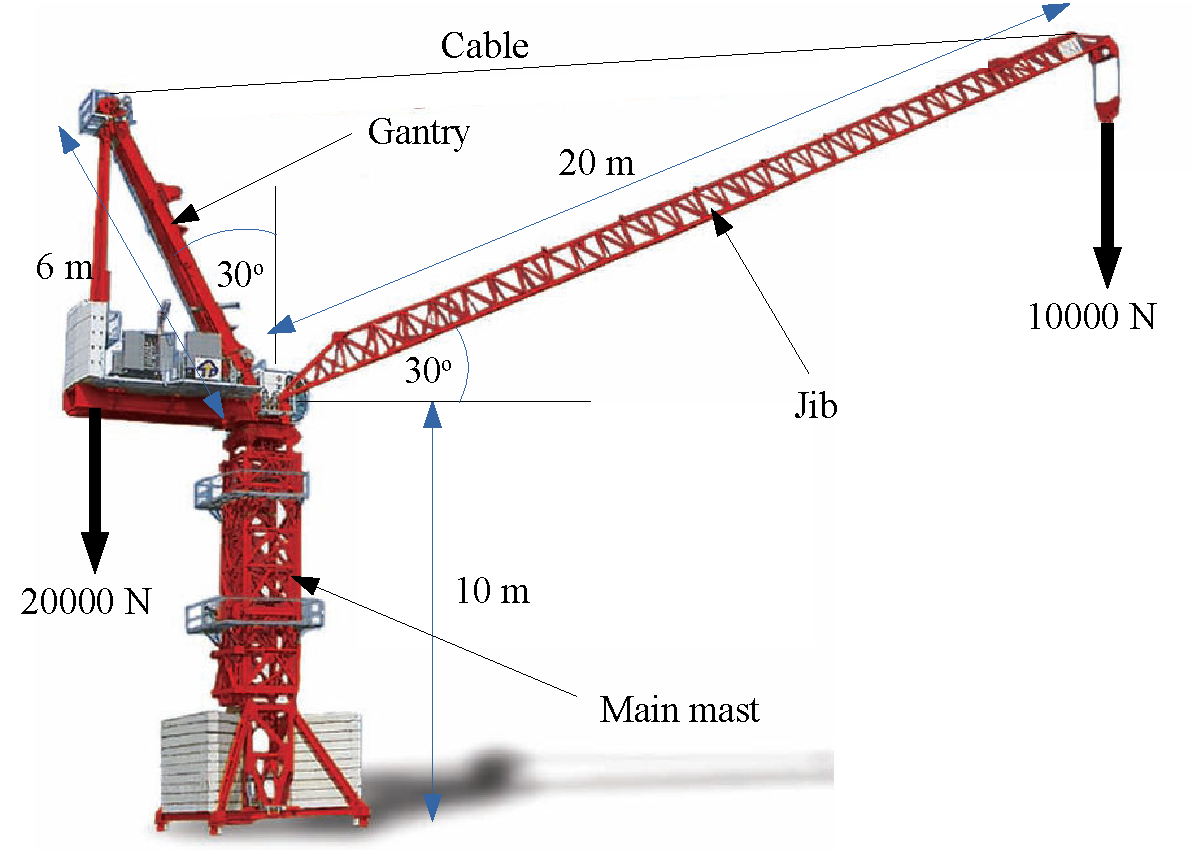
\includegraphics[scale=0.6]{pictures/Simple-load-bearing/tower-crane2}
    \caption{a typical luffing crane}
    \label{tower crane}
  \end{figure}
  
  As illustrated in \cref{tower crane}, a luffing crane typically consists of a main mast, a jib, a gantry and a counterweight. The jib and the gantry are \emph{always} perpendicular, but the jib can vary in angle with the horizontal line. In this problem, however, we will consider it fixed at 30$^{\circ}$. The counterweight is pulling directly downward on the end of the gantry, which is also connected to the end of the jib by a cable. The gantry is pinned to the top of the main mast.
  
  In reality, the main mast and jib are made of multiple short columns and beams welded together into a compound structure. For this problem, however, we will assume that the mast and jib are each made of a single constant cross-section steel. The steel has $E$ = 210 GPa, $S_y$ = 400 MPa, and $S_{ut}$ = 550 MPa.
  
  In this problem, the main mast is 10 m long, the jib is 20 m long, and the gantry is 6 m long. The counterweight weighs 20000 N. The angle $\theta = 30^{\circ}$. The maximum weight that the crane can lift is 10000 N. The safety factors of the mast and the jib are 2 and 3, respectively. The jib can be considered fixed to the mast, while the mast base is fixed to the ground and free to move at the top.
  
  Determine the required section modulus $S_{mast}$ and $S_{jib}$ and moments of inertia $I_{mast}$ and $I_{jib}$ of the mast and the jib. Ignore fatigue and stress concentration factors. You may assume that the mast, jib, and gantry are weightless.
  
\end{example}
\begin{solution}

  First order of business, we need to determine the load on the mast and the jib. Using free body diagrams, let us first start off with the gantry.
  
  On the gantry, since it is pinned to the mast, the only load from the top of the mast is along the length of the gantry. Consider balance of moments about the pinned joint, we have
  
  \begin{align*}
    20000(6 \sin 30^{\circ}) &= T \left( 6 \frac{20}{\sqrt{ 20^2 +6^2 }} \right) \\
    T &= 20880 \text{ N}
  \end{align*}

  The cable tension is 20880 N. We can find the moment applied at the fixed joint of the jib and the mast.
  
  \begin{align*}
    M_{jib} &= 20880 \left( \frac{6}{\sqrt{20^2 + 6^2}} \right) (20) - 10000(20 \cos 30^{\circ}) \\
            &= -53208 \text{ N-m}
  \end{align*}
  
  The bending moment the mast exerts on the jib is 53208 N-m (counterclockwise).
  
  We can also determine the axial load in the jib, which is

  \begin{align*}
    F_{jib} &= 20880 \left( \frac{20}{\sqrt{20^2 + 6^2}} \right) + 10000 \sin 30^{\circ} \\
            &= 25000 \text{ N}
  \end{align*}
  
  We can determine the required $I_{jib}$ and $S_{jib}$ now that we know the moments and load applied to the jib.
  
  The $S_{jib}$ is determined by the stress requirement. The maximum stress in the jib is at the bottom surface where the compressive bending stress and compressive axial stress combine. We have
  
  \begin{align*}
    N_s &= \frac{S_y}{\sigma_{axial} + \sigma_{bending}} \\
    3 &= \frac{400 \times 10^6}{\dfrac{25000}{A_{jib}} + \dfrac{53208}{S_{jib}}} \\[1ex]
    S_{jib} &= \frac{53208}{133 \times 10^6 - \dfrac{25000}{A_{jib}}}
  \end{align*}

  The $I_{jib}$ can be determined by the safety factor for buckling. We have
  
  \begin{align*}
    N_s &= \frac{P_{cr}}{P} \\
    3 &= \frac{ \pi^2 E I_{jib} }{ (2(20))^2 25000 } \\
    I_{jib} &= 5.79 \times 10^{-5} \text{ m}^4
  \end{align*}
  
  Now, the axial load in the mast can be easily determined. It is simply equal to the sum of all the external load = 20000 + 10000 = 30000 N (compressive).
  
  The only external moment applied to the mast is from the jib, and so the moment on the mast is equal and opposite to the moment on the jib = 53208 N-m (clockwise). The critical point is on the right side of the mast where compressive stresses from bending and axial load combine.
  
  The $S_{mast}$ and $I_{mast}$ can be found in similar fashion.
  
  \begin{align*}
    N_s &= \frac{S_y}{\sigma_{axial} + \sigma_{bending}} \\
    2 &= \frac{400 \times 10^6}{\dfrac{30000}{A_{mast}} + \dfrac{53208}{S_{mast}}} \\
    S_{mast} &= \frac{53208}{200 \times 10^6 - \dfrac{30000}{A_{mast}}} 
  \end{align*}
  
  \begin{align*}
    N_s &= \frac{P_{cr}}{P} \\
    2 &= \frac{ \pi^2 E I_{mast} }{ (2(10))^2 30000 } \\
    I_{mast} &= 1.16 \times 10^{-5} \text{ m}^4
  \end{align*}
  
  Note that the problem did not indicate the cross section shape of the mast and
  jib. If it did, the section moduli $S_{jib}$ and $S_{mast}$ can be solve
  analytically. On the other hand, the moments of inertia $I_{jib}$ and $I_{mast}$ can be solved without that information.
\end{solution}

\section*{Summary}

This chapter discusses the design criteria for simple load-bearing members—namely beams (for bending loads), shafts (for torques), and columns (for compressive loads). These are important building blocks for mechanical designs. They bear weights, transfer torques, and provide structural strength to parts. Fully understanding different types of loads and resultant state of stresses are keys to well-designed load bearing elements. A designer must also take care to examine risks for various types of failure a member may undergo, examine the most likely type of failure of that component, and properly design to mitigate it.

\section*{Exercises}

\begin{exercises}
  \exercise A 2-m long square ($a \times a$) cross-sectioned oak wood column ($E$ = 12 GPa, $S_{uc}$ = 12 MPa) is to take the compressive load of 50000 N. It is fixed at the bottom and free to move at the top. Determine the minimum required cross-sectional area so that the safety factor is 2.

  \begin{figure}[H]
    \centering
    \begin{tikzpicture}
      \node[draw, rectangle, fill=SkyBlue, minimum height=7cm, minimum width=0.5cm](A){};
      \draw[<-] (A.north) -- ++(90:1) node[above]{$P = 50000$ N};
      \node at (A.south) [anchor=north, rectangle, pattern=north east lines, minimum height=1cm, minimum width=2cm]{};
      \draw[fill=SkyBlue] (2,0) rectangle ++(1,1) node[midway]{$a \times a$};
    \end{tikzpicture}
  \end{figure}
  
  \exercise A 2-m long springboard is made of AISI1040 whose yield strength is 400 MPa and ultimate tensile strength is 650 MPa. The board cross section is rectangular with the base of 50 cm. If the maximum weight of a person allowed is 150 kg. Determine the proper thickness of the springboard under these criteria.

    \begin{figure}[H]
    \centering
    \begin{tikzpicture}
      \node[pattern=north west lines, minimum height=1.5cm, minimum width=1cm](wall){};
      \node at (wall.east) [anchor=west, draw, fill=SkyBlue, minimum height=2.5mm, minimum width=6cm](board){};
      \node at (board.north east) [anchor=south, draw, fill=Grey, minimum height=1cm, minimum width=5mm](person){}; 
      \node at (person.west) [left]{150 kg};
      % cross section
      \node at (board.east) [anchor=west, xshift=1cm, draw, fill=SkyBlue, minimum height=2.5mm, minimum width=3cm](boardsect){};
      \draw[|<->|] (boardsect.north west) ++ (90:0.3) --++(0:3) node[midway, fill=White]{50 cm};
      \draw[|<-] (boardsect.north east) ++ (0:0.3) --++(90:0.5) node[above]{$h$};
      \draw[|<-] (boardsect.south east) ++ (0:0.3) --++(-90:0.5);
    \end{tikzpicture}
  \end{figure}
  
  \begin{enumerate}
  \item Static loading. No jumping on the board.
  \item Impact loading. Assume the diver can jump 0.5 m from the horizontal level of the board.
  \item Fatigue loading. Assume the diver jumps 1 m up and down repeatedly on the board.
  \end{enumerate}
  
  \exercise A shaft fitted with pulley and belt is used to transmit engine power. The shaft is made of AISI1023 with yield strength of 400 MPa and ultimate tensile strength of 650 MPa. The belt tensions on the tight and slack sides are 4000 and 1000 N respectively. The pulley’s diameter is 10 cm. Size the shaft under

  \begin{figure}[H]
    \centering
    \begin{tikzpicture}
      \node at (0,0) [ellipse, draw, fill=LightGrey, rotate=-30, minimum height=2cm, minimum width=0.8cm]{};
      \node [anchor=west,cylinder, fill=LightBlue, draw, rotate=-30, minimum height=3.5cm, minimum width=1cm] (c){};
      \node at (c.east) [ellipse, draw, fill=LightGrey, rotate=-30, minimum height=3cm, minimum width=1.2cm](b){};
      \node at (b) [anchor=west,cylinder, fill=LightBlue, draw, rotate=-30, minimum height=3.5cm, minimum width=1cm](d){};
      \node at (d.east) [ellipse, draw, fill=LightGrey, rotate=-30, minimum height=2cm, minimum width=0.8cm]{};
      \draw [->, very thick] (b.north west) -- ++(-150:4) node[below left]{4000 N};
      \draw [->, very thick] (b.south east) -- ++(-150:4) node[below left]{1000 N};
    \end{tikzpicture}
  \end{figure}
  
  \begin{enumerate}
  \item static loading.
  \item fatigue loading.
  \end{enumerate}

  \exercise \label{exercise: footbridge} A footbridge is made of a series of columns, rails, and planks. A simplified section of the bridge is shown in \cref{fig: footbridge exercise}.

  \begin{figure}[H]
    \centering
    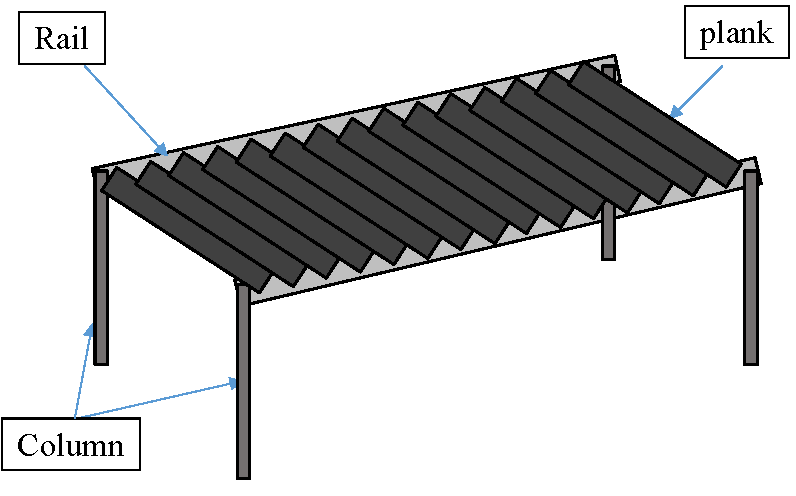
\includegraphics[scale=0.8]{pictures/Simple-load-bearing/footbridge}
    \caption{a footbridge for exercise \ref{exercise: footbridge}}
    \label{fig: footbridge exercise}
  \end{figure}
  
  The columns, rails, and planks are all made of Rosewood, a brittle material, which has $E$ = 10 GPa, ultimate tensile stress = 6 MPa, and ultimate compressive stress = 60 MPa. The columns are to be 3 m tall, the rails are to be 10 m long, and the planks are 2 m long. All supports can be considered simply supported or pinned. Assume that when a pedestrian uses the bridge, both of his feet will be on only one plank at a time, and that there will be only one pedestrian using the bridge at any moment. The maximum allowable weight of a person to cross the bridge is 2000 N and you may assume that the columns, rails, and planks are weightless.
  \begin{enumerate}
  \item Determine the type of deformation in each component when there is a pedestrian using the bridge.
  \item Draw a free body diagram of each component when there is a maximum load applied to it. (Show the magnitudes and directions of the loads)
  \item If the columns have circular cross sections, while the rails and planks have square cross sections, determine the diameter of the columns and the sizes of the cross section of the rails and planks so that the safety factor of the columns, rails, and planks are 10, 5, and 4, respectively. You may ignore fatigue failure.
  \item If a child comes to play on this bridge everyday by jumping repeatedly on the middle of a single plank, causing the maximum downward load on the plank of 1500 N, recalculate the proper cross section size of the plank so that the fatigue safety factor is 4.
  \end{enumerate}
\end{exercises}

%%%%%%%%%%%%%%%%%%%%%%%%%%%%%%%%%%%%%%%%%%%%%%%%%%%%%%%%%%%%%%%%%%%%%%%%%%%%%%%%%%%%%%%%%%%%%%%%%%%%%%%%%%%%%%%%%%%%%%%%%%%%%%%%%%%%%%%%%%%%%%%%%%%%%%%%%%%%%%%%%%%%%%%%%%%%%%%%%%%%%%%%%%%%%%%%%%%%%%%%%%%%%%%%%%%%%%%%%%%%%%%%%

\chapter{Spring Design}

Springs are elastic members that exert forces and torques and absorb energy, which is usually stored and later released. Typically they are made of metal, but can also be made from plastic for light loads. Even blocks of rubber are in fact springs, as in automobile bumpers and isolation mountings. There are also pneumatic springs of various types which uses the elastic compressibility of gases. For applications requiring compact springs providing very large forces with small deflections, hydraulic springs are very effective.

The main concern in this chapter is with springs made of solid metals, plastics, or composites. The following sections are concerned with springs of common geometric forms.

Various applications require flexibility and load control that springs provide. Springs come in many shapes and forms to provide forces and moments. There are also specialized types of springs for very specific applications. Here are some of the most prevalent ones in use.
\begin{enumerate}
\item Torsion bars: take axial twisting loads.
\item Helical springs: take tensile or compressive loads along the helix axis.
\item Leaf or beam springs: rely on beam bending.
\item Torsion springs: rely on bending of coiled wires.
\end{enumerate}
These are by no means an exhaustive list, but this book’s main focus will be on these four as a starting point.

\section{Torsion Bar Springs}

Perhaps the simplest of all the spring forms is the torsion bar. Common applications include part of automotive suspension springs and counter balancing springs for car hoods and trunk lids. A typical torsion bar spring suspension assembly is illustrated in \cref{fig: torsion bar spring}. These spring rely on elastic deformation under torsion to store and release strain energy.

\begin{figure}[h]
  \centering
  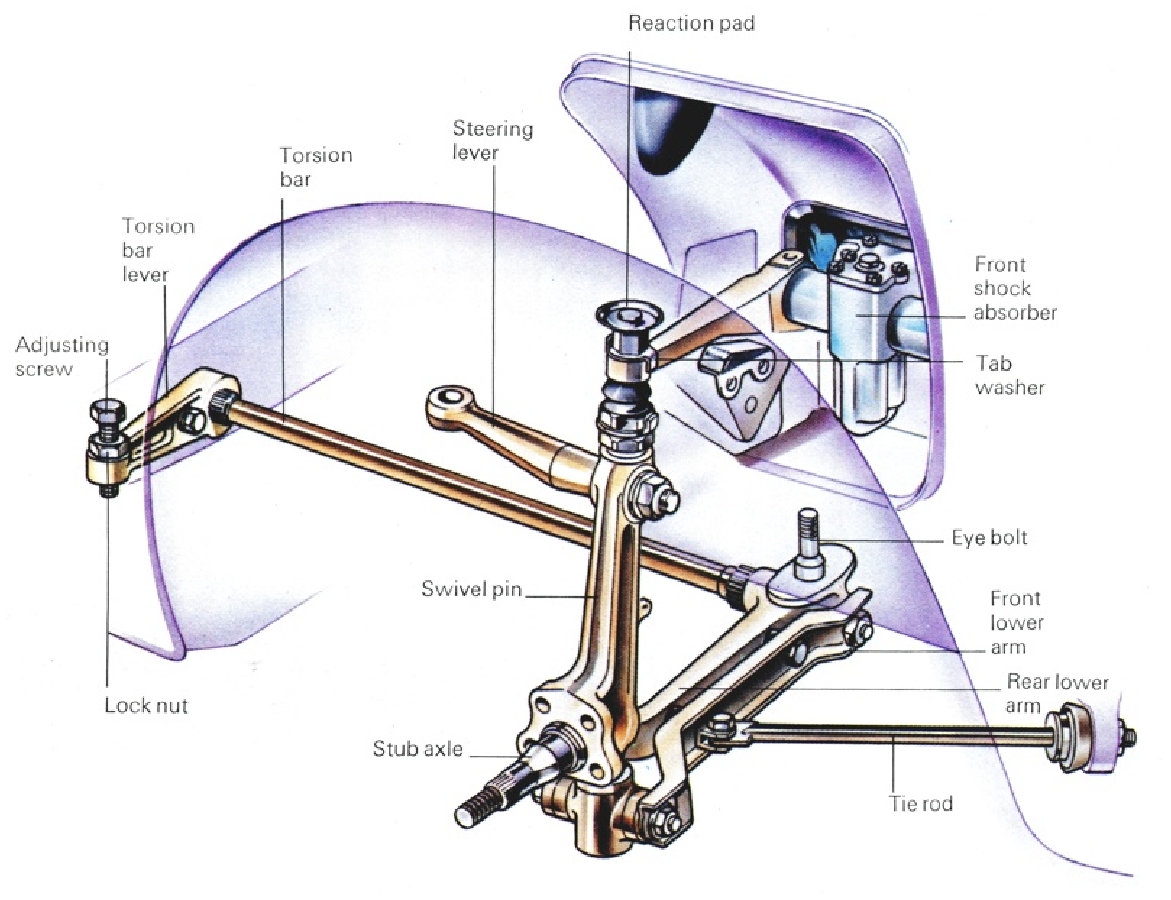
\includegraphics[scale=0.75]{pictures/Spring-design/torsion-bar-spring}
  \caption{Torsion bar spring suspension system}
  \label{fig: torsion bar spring}
\end{figure}

\subsection{Torsion Bar Spring Stress and Deformation}

In this case, the basic stress, angular deflection (or angle of twist), and spring rates equations are

\begin{equation}
  \begin{gathered}
    \tau  = \frac{Tr}{J} \hfill \\
    \phi  = \frac{TL}{GJ} \hfill \\
    k = \frac{T}{\phi} = \frac{GJ}{L} \hfill \\ 
  \end{gathered}
\end{equation}

For a solid round rod of diameter $d$, these become

\begin{equation}
  \begin{gathered}
    \tau  = \frac{16T}{\pi d^3} \hfill \\
    \phi  = \frac{32TL}{\pi d^4G} \hfill \\
    k = \frac{\pi d^4G}{32L} \hfill \\ 
  \end{gathered}
\end{equation}

\subsection{Torsion Bar Spring Materials}

As expected, torsion bar springs--especially in automotive suspension applications--tend to incur repeated loadings during operation. As such, steels remain the staple material of choice due to their endurance limits.

One of the most prevalent steels for torsion bar springs is AISI 8650H. It has been annealed at 800$^{\circ}$C and tempered at 500$^{\circ}$C to obtain its high strength and reasonable flexibility. Its properties are as follows.

\begin{description}
\item[Young's modulus] 205 GPa
\item[Shear modulus] 80 GPa
\item[Yield strength] 1076 MPa
\item[Ultimate tensile strength] 1255 MPa
\end{description}

\begin{example} Torsion bar spring design for a pick-up truck

  We want to design a torsion bar spring for a rear suspension of a pick-up truck which has to carry the maximum load of 20000 N. At this load, the chassis of the truck should not lower by more than 3 cm. The bar is connected to the chassis by a 6-cm lever. The bar itself is 30 cm long.
  
\end{example}
\begin{solution}

  In reality, a torsion bar spring is connected to multiple component to form a suspension system. All of these components will contribute the the vertical deflection of the chassis. In this problem, however, we will assume that the only source of vertical deflection comes from the rotation of the lever connected to the end of the torsion bar spring.

  To limit the vertical deflection to 3 cm, we must limit the angle of twist of the torsion bar. We will use AISI 8650H for the spring material.

  \begin{align*}
    \phi &= \frac{32TL}{\pi d^4 G} \\
    \frac{0.03}{0.06}  &= \frac{32(20000)(0.06)(0.3)}{\pi d^4 (80 \times 10^9)} \\
    d &= 1.74 \times 10^{-2} \text{ m}
  \end{align*}

  We must also verify that the designed torsion bar will not fail due to excessive shear stress. Therefore, we find the required spring diameter for strength and compare it to the designed diameter.

  Assuming that the torsion bar is in pure torsion, we find the maximum shear stress in order to determine the stress amplitude for fatigue analysis.

  \begin{align*}
    \tau  &= \frac{16T}{\pi d^3} \\
          &= \frac{16(20000)(0.06)}{\pi d^3} \\
          &= \frac{6111}{d^3}
  \end{align*}

  In pure torsion, the material is under pure shear. Using stress transformation (or Mohr's circle) to determine the equivalent normal stress, we have the maximum stress.

  \begin{gather*}
    \sigma_{\max} = \tau = \frac{6111}{d^3}
  \end{gather*}

  The minimum stress on the torsion bar spring is assumed to be zero, in which case the stress amplitude and average stress are

  \begin{align*}
    \sigma_a &= \frac{6111/d^3 - 0}{2} = \frac{3056}{d^3} \\
    \sigma_m &= \frac{6111/d^3 + 0}{2} = \frac{3056}{d^3}
  \end{align*}

  Substituting these values into Soderberg relation, we can solve for the required diameter for the assumed safety factor of 2.

  \begin{gather*}
    \frac{\sigma_a}{S_e} + \frac{\sigma_m}{S_y} = \frac{1}{N_s} \\
    \frac{3056/d^3}{0.3(1255 \times 10^6)} + \frac{3056/d^3}{1076 \times 10^6} = \frac{1}{2} \\
    d = 2.80 \times 10^{-2} \text{ m}
  \end{gather*}

  In this problem, the diameter according to the stress requirement is the larger one, and is our final design diameter.
\end{solution}
  
\section{Helical Springs}

Helical springs employ the same principles as torsion bar springs, but avoid the problem of size by winding the spring into helical coils. Helical springs still operate mainly under torsion, however, their stresses are different from their torsional bar counterparts because of their geometry.

\subsection{Helical Spring Stress}

Consider helical coil springs with relatively small helix angle and wire diameter d, illustrated in \cref{fig: helical spring geometry}. At each end of the spring, external force F is applied along the axis of the helix. In compression springs, this is accomplished by winding the end coils with zero pitch and grinding the ends flat to insure uniformly distributed load at end plates. In the tension spring, the end hooks are formed to position the load along the axis.

\begin{figure}[h]
  \centering
  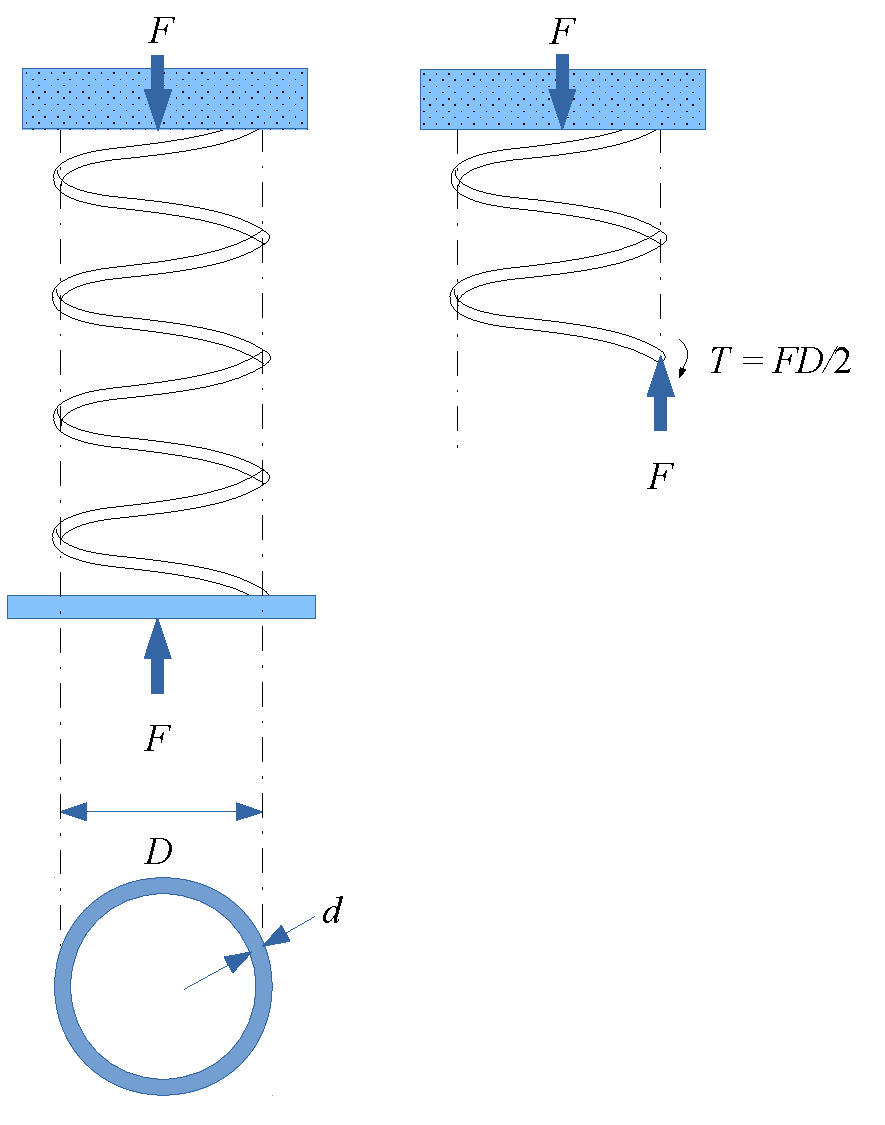
\includegraphics[scale=0.55]{pictures/Spring-design/helical-spring-geometry}
  \caption{Helical spring geometry and loading conditions.}
  \label{fig: helical spring geometry}
\end{figure}

Regardless of where the cutting plane takes place, equilibrium considerations require that the wire be subjected to (1) a transverse shear force $F$ and (2) a torque equal to $FD/2$. The resultant shear stress is

\begin{align*}
  \tau  &= \tau_{shear} + \tau_{torsion} \\ 
        &= \frac{Tr}{J} + \frac{F}{A} \\
\end{align*}
\begin{align*}
  &= \dfrac{\dfrac{FD}{2}\dfrac{d}{2}}{\dfrac{\pi}{2}\left( \dfrac{d}{2} \right)^4} + \dfrac{F}{\dfrac{\pi d^2}{4}} \\ 
  &= \frac{8FD}{\pi d^3} + \frac{4F}{\pi d^2} 
\end{align*}

Note that the second term is relatively small.

However, because of the curvature of the coil, the torsional stress on its surface is increased. The severity of this effect is greatest when the spring index $C$, defined as the ratio of mean coil diameter $D$ to wire diameter $d$.

\begin{equation}
  C = \frac{D}{d}
\end{equation}

The first generally recognized analysis of the transverse shear and curvature effects was published by A. M. Wahl in 1929. This analysis involved the derivation of the equation for a factor Kw (now called Wahl factor) by which the stress can be multiplied to give the total resultant shear stress on the inside of the coil.

\[K_w = \frac{4C - 1}{4C - 4} + \frac{0.615}{C}\]

Another correction factor is derived by Bergstrasser, which provides a simpler equation with relatively small errors ($< 1\%$).

\begin{equation}
  K_b = \frac{4C + 2}{4C - 3}
\end{equation}

These factors can be multiplied with the torsional shear stress term to give the approximate resultant shear stress of the inside of the spring coil. In this book, however, Bergstrasser will be used due to its simpler expression.

\begin{equation} \label{eqn: spring torsional stress}
  \tau  = K_b\frac{8FD}{\pi d^3}
\end{equation}

\subsection{Helical Spring Constant and Deflection}

Derivation of spring deflection can be done using Castigliano’s theorem. By assuming that transverse shear contributes negligibly to the deflection, only the torsional load is considered. According to the theorem, we have

\[\delta  = \int_0^L \frac{T}{GJ}\left( \frac{\partial T}{\partial F} \right)dx\]

Substitute the values for each parameter and let $N_a$ be the number of active coils, we have

\begin{align*}
  \delta  &= \int_0^{2\pi N_a} \left( \frac{32}{G\pi d^4} \right)\left( \frac{FD}{2} \right)\left( \frac{D}{2} \right)\left( \frac{D}{2}d\theta  \right) \\ 
          &= \frac{4FD^3}{\pi d^4G} \\ 
          &= \frac{8FD^3N_a}{d^4G}
\end{align*}

The spring constant or spring rate is the ratio between the axially applied force and the deflection, which gives

\begin{equation} \label{eqn: spring constant}
  \begin{gathered}
    k = \frac{F}{\delta} = \frac{d^4G}{8D^3N_a} \hfill \\
    \text{or} \hfill \\
    k = \frac{Gd}{8C^3N_a} \hfill \\ 
  \end{gathered}
\end{equation}

\subsection{Analysis for Helical Compression Springs under Static Loading}

Helical springs are typically wound from wire of solid round cross section. Although spring wire was formerly manufactured primarily in certain gage diameters, it is now readily available in any desired size, though manufacturers may only stock certain preferred sizes.

The basic concern when designing springs for static loading is to avoid set, which is a long-term shortening of the spring under load. For helical springs, set is directly related to maximum allowable shear stress—shear stress that leads to yielding. As a general rule of thumb, fewer than 2\% of springs will experience long-term set if the shear stress is equal to 45\% of ultimate tensile strength for ferrous spring, and 35\% for nonferrous and stainless steel springs.

\begin{equation}
  \tau_{allow} \leqslant \left\{
    \begin{array}{ll}
       0.45 S_{ut} & \text{ferrous} \hfill \\ 
       0.35 S_{ut} & \text{nonferrous and stainless} 
     \end{array} \right.
\end{equation}

Ultimate tensile stresses of wire materials have been experimentally determined and formulated as follows.

\begin{equation} \label{eqn: spring material strength}
  S_{ut} = \frac{A}{d^m}
\end{equation}

Special care must be taken when using \cref{eqn: spring material strength} in conjunction with other equations for spring design. The units of $S_{ut}$, $A$, and $d$ in the equation are MPa-mm and mm, respectively. So they must be converted to their correct units before using in other SI-oriented equations presented elsewhere.

The values for $A$ and exponent $m$ for various wire materials are shown in \cref{table: spring materials}.

\begin{table}[h] 
  \centering
  \caption{Strength and relative cost parameters for various spring wire materials.} \label{table: spring materials}
  \begin{tabular}{ L{3cm} C{2cm} C{2cm} C{2cm} C{2cm} C{2cm} }
    \toprule
    Material & Diameter (mm) & G (GPa) & A (MPa-mm) & m & Relative Cost \\
    \midrule
    Music & 0.1 – 6.5 & 81.7 & 2211 & 0.145 & 2.6 \\
    \midrule
    OQ\&T & 0.5 – 12.7 & 77.2 & 1855 & 0.187 & 1.3 \\
    \midrule
    Hard-drawn & 0.7 – 12.7 & 79.3 & 1783 & 0.190 & 1.0 \\
    \midrule
    Chrome-vanadium & 0.8 – 11.1 & 77.2 & 2005 & 0.168 & 3.1 \\
    \midrule
    Chrome-silicon & 1.6 – 9.5 & 77.2 & 1974 & 0.108 & 4.0 \\
    \midrule
    \multirow{3}{3cm}{302 stainless steel} & 0.3 – 2.5 & \multirow{3}{2cm}{\centering 69} & 1867 & 0.148 & \multirow{3}{2cm}{\centering 7.6 – 11} \\
    & 2.5 – 5 & & 2065 & 0.263 & \\
    & 5 – 10 & & 2911 & 0.478 & \\
    \midrule
    \multirow{3}{3cm}{Phosphor-bronze} & 0.1 – 0.6 & \multirow{3}{2cm}{\centering 41} & 1000 & 0 & \multirow{3}{2cm}{\centering 8.0} \\
    & 0.6 – 2 & & 913 & 0.028 & \\
    & 2 – 7.5 & & 932 & 0.064 & \\
    \bottomrule
  \end{tabular}
\end{table}

Besides the material strength, spring materials offer a variety of properties suitable for different operating conditions. \Cref{table: spring material properties} details specific properties of different spring materials.

\begin{table}[h]
  \centering
  \caption{Specific spring material characteristics.} \label{table: spring material properties}
    \begin{tabular}{ L{3cm} L{10cm}}
      \toprule
      Materials & Descriptions  \\
      \midrule
      Music & Strongest materials available for small springs. Excellent under repeated loadings. Do not use above 120 C or below 0 C. \\
      \midrule
      OQ\&T* & Good for general purpose springs where music wires may be too expensive or too small. Not for shock or impact loadings. Do not use above 180 C or below 0 C. \\
      \midrule
      Hard-drawn & Cheapest material for general purpose springs. Should only be used where accuracy, life, and deflection are unimportant. Do not use above 120 C or below 0 C. \\
      \midrule
      Chrome-vanadium & Most popular springs for higher stress than can be used with carbon steel springs and where fatigue resistance and longevity are needed. Also good under impact and shock loadings. Widely used for aircraft engine valve springs for up to 220 C. \\
      \midrule
      Chrome-silicon & Excellent under high stress and shock loadings, and provides good longevity. \\
      \bottomrule
    \end{tabular}
  \end{table}

\subsection{End Designs of Helical Compression Springs}

In order to ensure that the resultant load coincides with the spring axis, spring ends must be designed properly for their uses. This usually involves grinding and squaring the ends to keep nearly a full turn of wire in contact with end plates. These ground/squared coils do not contribute to spring flexibility and are not counted as \emph{active coils}. The exact numbers for different end conditions are illustrated in \cref{table: spring end conditions}. Note that the range (maximum deflection) of a spring regardless of its end type is equal to $np - nd$.

\begin{table}[h]
  \centering
  \caption{Number of active coils and lengths of different spring end conditions.} \label{table: spring end conditions}
    \begin{tabular}{ L{4.6cm} C{2.2cm} C{2.2cm} C{2.4cm} C{2.4cm} }
      \toprule
      \multirow{2}{3cm}{\centering \vspace{-0.7cm} Term} & \multicolumn{4}{c}{Type of spring end} \\ \cmidrule{2-5}
      & Plain & Plain and ground & Squared or closed & Squared and ground \\
      \midrule
      Number of end coils, $N_e$ & 0 & 1 & 2 & 2 \\
      Total number of coils, $N_t$ & $N_a$ & $N_a+1$ & $N_a+2$ & $N_a+2$ \\
      Free length, $l_f$ & $pN_a+d$ & $p(N_a+1)$ & $pN_a+3d$ & $pN_a+ 2d$ \\
      Solid length, $l_s$ & $d(N_t+1)$ & $d N_t$ & $d(N_t+1)$ & $dN_t$ \\
      pitch, $p$ & $(l_f - d)/N_a$ & $l_f/(N_a + 1)$ & $(l_f - 3d)/N_a$ & $(l_f - 2d)/N_a$ \\
      \bottomrule
  \end{tabular}
\end{table}

\subsection{Buckling Analysis of Helical Compression Springs}

Coil springs loaded in compression behave just like columns and must be considered for possible buckling. For columns, long and slender ones are considered prone to buckling; similar criteria apply to spring--springs with large free length and small coil diameter tend to buckle easily. Buckling, of course, also depends on exerted axial load and end conditions. In \cref{fig: spring buckling}, buckling stability of helical compression springs are shown. Intuitively, springs with parallel ends are much less prone to buckling than those with nonparallel ends. The $x$-axis indicates the stability of the spring due to its geometry, while the $y$-axis implicitly indicates the compressive load from the deflected length.

The governing equation for buckling stability can be written as

\begin{equation}
  L_f < \frac{\pi D}{\alpha} \left[ \frac{2(E-G)}{2G+E} \right]^{1/2}
\end{equation}

where

\begin{equation*}
  \alpha = \frac{KD}{L_f}
\end{equation*}

is the effective slenderness ratio, equivalent the same quantity for column buckling. Table \cref{table: spring buckling} gives the value $K$ for different end conditions. Notice how the values are identical to those of column buckling.

\begin{table}
  \centering
  {\renewcommand{\arraystretch}{1.2}
  \begin{tabular}{L{11cm} C{2cm}}
    \toprule
    End Condition & Constant $K$ \\
    \midrule
    Spring supported between flat parallel surfaces (fixed ends) & 0.5 \\
    One end fixed on flat surface; the other pinned & 0.707 \\
    Both ends pinned & 1 \\
    One end clamped; other end free & 2 \\
    \bottomrule
  \end{tabular}}
  \caption{Constants $K$ for helical compression springs under various end conditions.}
  \label{table: spring buckling}
\end{table}

\begin{figure}[h]
  \centering
  \begin{tikzpicture}
    \begin{axis}[
      height=10cm,
      width=10cm,
      axis background/.style={fill=SkyBlue!50},
      axis line style={->},
      grid=both,
      grid style={draw=Grey!10},
      xmin=1.5, xmax=10.5,
      xlabel={Free length to coil diameter ratio, $L_f / D$},
      ymin=0, ymax=0.8,
      ylabel={Deflection to free length ratio, $\delta / L_f$}]
      %% C1 = 0.79, C2 = 7.21
      
      \addplot [RoyalBlue,thick,domain=2:10,samples=200]{0.79*(1-sqrt(1-7.21/(0.5*\x)^2))} node[midway, xshift=4mm, yshift=3mm, black, rotate=-40]{Fixed ends};
      \addplot [RoyalBlue,thick, densely dotted,domain=2:10,samples=200]{0.79*(1-sqrt(1-7.21/(0.707*\x)^2))} node[midway, xshift=-5mm, yshift=-1mm, black, rotate=-30]{Fixed - free};
    \end{axis}
    \node at (5,5) {Unstable};
    \node at (1,2) {Stable};
  \end{tikzpicture}
  \caption{Buckling stability of helical springs.}
  \label{fig: spring buckling}
\end{figure}

Observe the graph in \cref{fig: spring buckling} that both curves appear to have $x$-axis asymptotes. These values are very important; below these $L_f/D$ ratios, springs will \emph{not} buckle regardless of exerted deflection. For steels, this turns out to be

\begin{equation}
  L_f < 2.63 \frac{D}{K}
\end{equation}

For squared and ground ends between flat parallel surfaces $K$ = 0.5 and $L_f < 5.26 D$.

\subsection{Design Procedure for Helical Compression Spring—Static Loading}

The two most basic requirements of a helical spring design are an acceptable stress level and the desired spring rate. To minimize weight, size, and cost, we usually design springs to the highest stress level that will not result in significant long-term set. Stress is typically considered first because it involves only $D$ and $d$.

In compression springs, there are two load-related design safety measures. The first of which is that designers must ensure that the spring will not fail during operation. While this seems like a general enough guideline for not only compression springs, one must recall that compression springs have hard stops, namely their solid lengths. Additional load exerted beyond solid force is unlikely to increase the torsional shear stress in the spring wire. This is also the reason safety factors in compression springs are usually on the small side ($N_s \geq 1.2$). The designers simply needs to ensure that the spring torsional stress at solid length is less than its allowable shear stress.

\begin{equation} \label{eqn: spring allowable stress}
  \begin{gathered}
    N_s = \frac{\tau _s}{\tau _{allow}} \hfill \\
    N_s \geqslant 1.2 \hfill \\ 
  \end{gathered}
\end{equation}

Applying equations for spring torsional shear stress—\cref{eqn: spring torsional stress}—and wire allowable shear stress—\cref{eqn: spring allowable stress}, we have

\begin{equation}
  \frac{\tau _{allow}}{N_s} = K\frac{8F_sD}{\pi d^3}
\end{equation}

The second design safety measure is to prevent the spring from reaching solid length. This is important in
\begin{enumerate}
\item keeping the spring from failure and
\item allowing smooth operation of the spring
\end{enumerate}
Once the spring reaches its solid length, it no longer behaves like a spring but rather a tube whose stiffness is much higher. The designer can prevent this by ensuring that the maximum compressive load applied to the spring is less than its solid force.

\begin{equation}
  \begin{gathered}
    F_{\max} < F_s \\ 
    F_s = F_{\max}(1 + \xi ) \\ 
    \xi  \geqslant 0.15 \\ 
  \end{gathered}
\end{equation}

Combining these two equations, we arrive at the final expression for spring torsional stress.

\[\frac{\tau _{allow}}{N_s} = \frac{8KF_sD}{\pi d^3} = \frac{4C + 2}{4C - 3}\left[ \frac{8(1 + \xi )F_{\max }C}{\pi d^2} \right]\]

Rearranging and reassigning parameters, the equation can be solved for spring index $C$.

\begin{equation}
  \begin{gathered}
    \alpha  = \frac{\tau_{allow}}{N_s} \\ 
    \beta  = \frac{8(1 + \xi )F_{\max}}{\pi d^2} \\ 
    C = \frac{2\alpha  - \beta }{4\beta} + \sqrt {\left( \frac{2\alpha  - \beta}{4\beta} \right)^2 - \frac{3\alpha}{4\beta}}  \\ 
  \end{gathered}
\end{equation}

In general, the stress requirement can be satisfied by many combinations of $D$ and $d$, and the objective is to find one that best suits the requirements of the particular problem. With $D$ and $d$ tentatively selected, $N_a$ is then determined on the basis of the required spring rate using \cref{eqn: spring constant}.

\begin{equation}
  N_a = \frac{Gd^4}{8D^3k} = \frac{Gd}{8C^3k}
\end{equation}

Finally, the free length of the spring is determined by what length will give the desired clash allowance. If the resulting design is prone to buckling, or if the spring does not fit into the available space, another combination of $D$ and $d$ may be selected. If the spring comes out too large or too heavy, a stronger material must be considered.

The process of helical compression spring design can be summarized by a process flowchart illustrated in \cref{fig: spring design flowchart}

\begin{figure}[h]
  \centering
  \begin{tikzpicture}
    \node[draw, rectangle, fill=LightSkyBlue, minimum height=1cm, minimum width=2cm, text width=2cm, align=center](1){Select \\ Material};
    \node at (1) [yshift=-1.5cm, draw, rectangle, fill=LightSkyBlue, minimum height=1cm, minimum width=2cm, text width=2cm, align=center](2){Stress \\ ($D$ and $d$)};
    \node at (2) [yshift=-1.5cm, draw, rectangle, fill=LightSkyBlue, minimum height=1cm, minimum width=2cm, text width=2cm, align=center](3){Stifness \\ $N_a$};
    \node at (3) [yshift=-2cm, draw, diamond, fill=LightSkyBlue, minimum height=1cm, minimum width=1.5cm, text width=2cm, align=center, aspect=2](4){Buckle?};
    \node at (4) [yshift=-2cm, draw, diamond, fill=LightSkyBlue, minimum height=1cm, minimum width=1.5cm, text width=2cm, align=center, aspect=2](5){Large?};
    \node at (5) [yshift=-2cm, draw, diamond, fill=LightSkyBlue, minimum height=1cm, minimum width=1.5cm, text width=2cm, align=center, aspect=2](6){Resonance?};
    \node at (6) [yshift=-2cm, draw, rectangle, fill=LightSkyBlue, minimum height=1cm, minimum width=2cm, text width=2cm, align=center](7){Finish};
    \draw [->] (1) -- (2);
    \draw [->] (2) -- (3);
    \draw [->] (3) -- (4);
    \draw [->] (4) -- (5) node[midway, right]{No};
    \draw [->] (5) -- (6) node[midway, right]{No};
    \draw [->] (6) -- (7) node[midway, right]{No};

    \draw [->] (4.east) --++ (0:1) node[midway, above]{Yes} --++ (90:3.5) -- (2);
    \draw [->] (5.east) --++ (0:1.5) node[midway, above]{Yes} --++ (90:7) -- (1);
    \draw [->] (6.east) --++ (0:1.6) node[midway, above]{Yes} --++ (90:9) -- (1);
  \end{tikzpicture}
  % 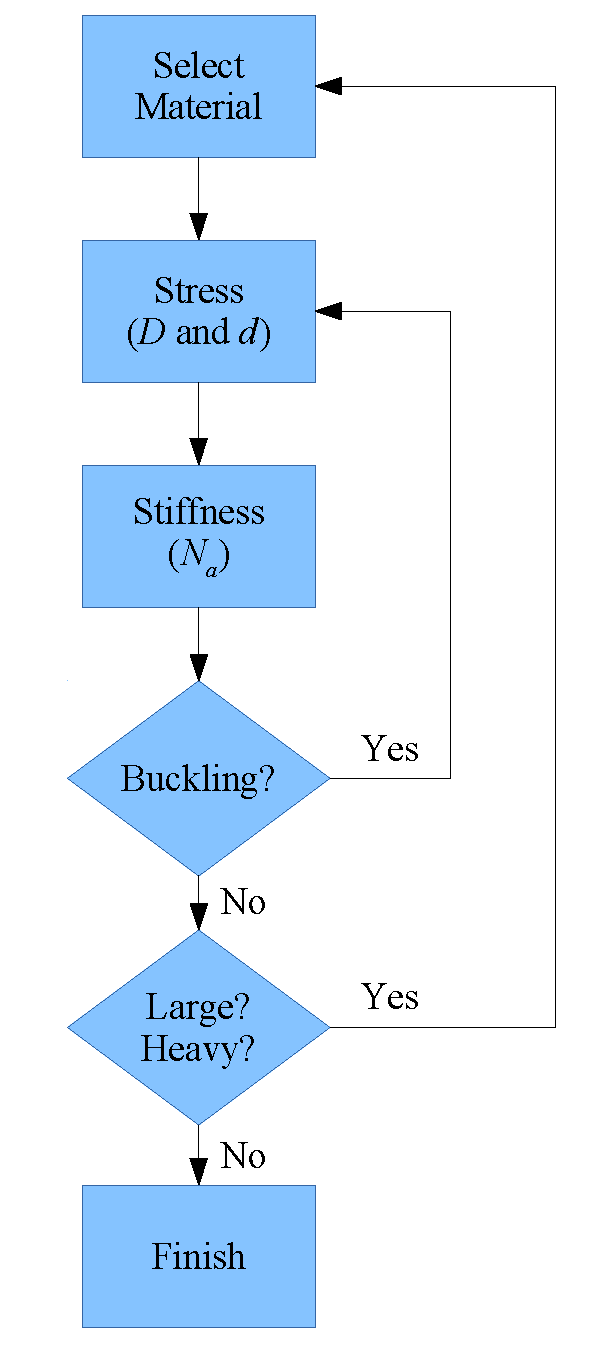
\includegraphics[scale=0.6]{pictures/Spring-design/spring-design-flowchart}
  \caption{Helical spring design process flowchart}
  \label{fig: spring design flowchart}
\end{figure}

The following general guidelines are provided for standard helical spring designs for static loading.

\begin{equation}
  \begin{gathered}
    4 \leqslant C \leqslant 12 \\ 
    3 \leqslant N_a \leqslant 15 \\ 
    N_s \geqslant 1.2 \\ 
    \xi  \geqslant 0.15 \\ 
  \end{gathered}
\end{equation}

The first inequality sets a range of spring index value for standard helical springs; if the index is too small the spring must be coiled extremely tight, too large and it is wound too loose. The second inequality provides a rough standard number of active coils. The final equation requires that the maximum compressive for the spring will take must be smaller than the solid force.

\begin{example} Design of bicycle suspension and seat springs

  Consider bicycle suspensions. The bike weighs 15 kg and its center of mass (CM) is shown below. After a 70-kg rider sits on the seat, the front suspension shrinks by 0.5 cm while the seat suspension shrinks by 1 cm. Determine the proper front and seat suspension springs. You may assume that both springs are vertical (not slanted) during operation.

\end{example}

\begin{solution}
  
  First, consider weight distribution in both springs without the rider. Obviously, since no one is riding, there is no load on the seat spring. On the front spring, we can determine the load using moment equilibrium and taking the rear wheel as a fulcrum. The equilibrium equation gives

  \[\begin{gathered}
      (0.4)(150) = F_f(1.2) \hfill \\
      F_f = 50 \text{ N} \hfill \\ 
    \end{gathered} \]

  Now consider the weight distribution with the rider. Again, the rider is sitting on top of the seat (and the seat spring), so his entire weight is supported by the seat spring. So $F_s$ = 700 N. The force in the front spring can be determined by equilibrium, which gives

  \[\begin{gathered}
      (0.2)(700) + (0.4)(150) = F_f(1.2) \hfill \\
      F_f = 167 \text{ N} \hfill \\ 
    \end{gathered} \]

  We can derive the required stiffness of each spring by combining the derived change in force and the prescribed deflection.

  \[\begin{gathered}
      k_f = \frac{167 - 50}{0.005} = 23400 \text{ N/m} \hfill \\
      k_s = \frac{700 - 0}{0.01} = 70000 \text{ N/m} \hfill \\ 
    \end{gathered} \]

  While the problem does not specify the required material, suspensions obviously will undergo repeated and impact loadings—especially since this is a mountain bike. A proper choice in this case would be Chrome-Vanadium or Chrome-Silicon, as it provides good fatigue and shock resistance. In this problem, we will go with Chrome-Vanadium ($A$ = 2005, $m$ = 0.168).
  
  Next, consider the stress limitation to select $D$ and $d$. By setting $N_s$ = 1.25 and $\xi$ = 0.15, if we choose $d$ = 2.5 mm for the front suspension, the spring index $C$ can be calculated.

  \begin{align*}
    \alpha  &= \frac{\tau _{allow}}{N_s} = \frac{0.45}{1.25}\frac{2005}{2.5^{0.168}} \times 10^6 = 619 \text{ MPa} \\ 
    \beta  &= \frac{8(1 + \xi )F_{\max}}{\pi d^2} = \frac{8(1 + 0.15)167}{\pi (2.5 \times 10^{-3})^2} = 78.2 \text{ MPa}
  \end{align*}
  \begin{align*}
    C &= \frac{2\alpha  - \beta}{4\beta} + \sqrt {\left( \frac{2\alpha  - \beta}{4\beta} \right)^2 - \frac{3\alpha}{4\beta}}  \\ 
      & = \frac{2(619) - 78.2}{4(78.2)} + \sqrt {\left( \frac{2(619) - 78.2}{4(78.2)} \right)^2 - \frac{3(619)}{4(78.2)}}  \\ 
      &= 6.5 
  \end{align*}

  Repeating the same procedure for the seat spring, setting the same safety measures and choosing $d$ = 5 mm.

  \begin{align*}
    \alpha &= \frac{\tau_{allow}}{N_s} = \frac{0.45}{1.25}\frac{2005}{5^{0.168}} \times 10^6 = 550\text{ MPa} \\ 
    \beta &= \frac{8(1 + \xi )F_{\max}}{\pi d^2} = \frac{8(1 + 0.15)700}{\pi (5 \times 10^{-3})^2} = 82\text{ MPa}
  \end{align*}
  \begin{align*}
    C &= \frac{2\alpha  - \beta}{4\beta} + \sqrt {\left( \frac{2\alpha  - \beta}{4\beta} \right)^2 - \frac{3\alpha}{4\beta}}  \\ 
      &= \frac{2(550) - 82}{4(82)} + \sqrt {\left( \frac{2(550) - 82}{4(82)} \right)^2 - \frac{3(550)}{4(82)}}  \\ 
      &= 5.24
  \end{align*}

  Apply the stiffness requirement to determine the required number of active coils.

  \begin{align*}
    N_{af} &= \frac{Gd}{8C^3k} = \frac{77.2 \times 10^9(2.5 \times 10^{-3})}{8(6.5^3)(23400)} = 3.75 \\
    N_{as} &= \frac{Gd}{8C^3k} = \frac{77.2 \times 10^9(5 \times 10^{-3})}{8(5.24^3)(70000)} = 4.79
  \end{align*}

  To determine the pitches, and thus the spring lengths, we will assume that the spring ends are squared and ground so that both are parallel. The maximum deflections of the front and seat springs are

  \begin{align*}
    \delta_f &= \frac{F_f}{k_f} = \frac{167}{23400} = 7.14 \times 10^{-3} \text{ m} \\
    \delta_s &= \frac{F_s}{k_s} = \frac{700}{70000} = 1 \times 10^{-2}\text{ m}
  \end{align*}

  As a general rule of thumb the maximum deflection should not exceed 80\% of the spring compression range, which is $N_a(p - d)$, the designed pitches for the front and seat springs are

  \[\frac{\delta}{N_a(p - d)} = 0.8\]

  For the front suspension spring pitch,

  \begin{align*}
    p_f &= \frac{\delta _f}{0.8N_{af}} + d_f \\ 
          &= \frac{7.14 \times 10^{-3}}{0.8(6.5)} + 2.5 \times 10^{-3} \\ 
          &= 3.87 \times 10^{-3} \text{ m}
  \end{align*}

  And similarly, for the seat spring pitch,

  \begin{align*}
    p_s &= \frac{\delta _s}{0.8N_{as}} + d_s \\ 
          &= \frac{1 \times 10^{-2}}{0.8(5.24)} + 5 \times 10^{-3} \\ 
          &= 7.39 \times 10^{-3}\text{ m}
  \end{align*}
\end{solution}

\begin{example} An 1200-kg empty car with the following dimensions stands 15 cm from the ground both in the front and the rear. However, when it is fully loaded by adding 150 kg to the front seats and 200 kg to the back seats, the front and the rear stand 13 cm and 12 cm from the ground, respectively. Design the front and rear springs for the suspension system of this car. 
\end{example}
\begin{solution}
First, we need to find the maximum load in the front and rear suspension. Use static equilibrium. For the empty car

   \begin{align*}
     2F_{r1}(2595) &= 12000(1050) \\
     F_{r1} &= 2428 \text{ N} \\
     2F_{f1} &= 12000 - 2(4856) = 7144 \\
     F_{f1} &= 3572 \text{ N}
   \end{align*}

   For the fully loaded car, the added front load goes at the c.g., while the read load goes in the middle of c.g. and rear wheel. The distance from the rear load to the rear wheel is

   \begin{gather*}
     d_r = \frac{2595 - 1050}{2} = 772.5 \text{ mm}
   \end{gather*}

   The front and rear loads in the fully loaded car are

   \begin{align*}
     2F_{f2}(2595) &= (12000 + 1500)(2595 - 1050) + 2000(772.5) \\
     F_{f2} &= 4316 \text{ N} \\
     2F_{r2} &= 12000 + 1500 + 2000 - 2(4316) \\
     F_{r2} &= 3434 \text{ N}
   \end{align*}

   With known loads, we can determine the spring $C$ from stress equation. First, the front springs. By setting $N_s$ = 1.25 and $\xi$ = 0.15, if we choose $d$ = 15 mm for the front suspension, the spring index $C$ can be calculated.

   \begin{align*}
    \alpha &= \frac{\tau_{allow}}{N_s} = \frac{0.5}{1.25}\frac{2005}{15^{0.168}} \times 10^6 = 509 \text{ MPa} \\ 
    \beta &= \frac{8(1 + \xi)F_{\max}}{\pi d^2} = \frac{8(1 + 0.15)4316}{\pi (15 \times 10^{-3})^2} = 56.2 \text{ MPa}
  \end{align*}
  \begin{align*}
    C &= \frac{2\alpha  - \beta}{4\beta} + \sqrt {\left( \frac{2\alpha  - \beta}{4\beta} \right)^2 - \frac{3\alpha}{4\beta}}  \\ 
      & = \frac{2(509) - 56.2}{4(56.2)} + \sqrt {\left( \frac{2(509) - 56.2}{4(56.2)} \right)^2 - \frac{3(509)}{4(56.2)}}  \\ 
      &= 7.7 
  \end{align*}

  We perform the same calculation for the rear springs. Pick $d$ = 13 mm since the maximum force is slightly smaller than the front springs.

   \begin{align*}
     \alpha &= \frac{\tau_{allow}}{N_s} = \frac{0.5}{1.25}\frac{2005}{13^{0.168}} \times 10^6 = 521 \text{ MPa} \\ 
    \beta &= \frac{8(1 + \xi)F_{\max}}{\pi d^2} = \frac{8(1 + 0.15)3434}{\pi (13 \times 10^{-3})^2} = 59.5 \text{ MPa}
  \end{align*}
  \begin{align*}
    C &= \frac{2\alpha  - \beta}{4\beta} + \sqrt {\left( \frac{2\alpha  - \beta}{4\beta} \right)^2 - \frac{3\alpha}{4\beta}}  \\ 
      & = \frac{2(521) - 59.5}{4(59.5)} + \sqrt {\left( \frac{2(521) - 59.5}{4(59.5)} \right)^2 - \frac{3(521)}{4(59.5)}}  \\ 
      &= 7.4 
  \end{align*}

  $D$ of the front and rear springs can be easily calculated

  \begin{align*}
    D_f &= Cd = 7.7(15) = 116 \text{ mm} \\
    D_r &= 7.4(13) = 96.2 \text{ mm}
  \end{align*}

  Spring constants is needed to determine the required number of active coils $N_a$.
  \begin{align*}
    k_f &= \frac{\Delta F}{\Delta x} = \frac{4316 - 3572}{0.02} \\
        &= 37200 \text{ N/m} \\
    k_r &= \frac{3434 - 2428}{0.03} \\
        &= 33533 \text{ N/m}
  \end{align*}

  Determine the $N_a$

  \begin{align*}
    N_{af} &= \frac{Gd}{8C^3k} = \frac{77.2 \times 10^9(15 \times 10^{-3})}{8(7.7^3)(37200)} = 8.6 \\
    N_{ar} &= \frac{Gd}{8C^3k} = \frac{77.2 \times 10^9(13 \times 10^{-3})}{8(7.4^3)(33533)} = 9.3 \\
  \end{align*}

Determine pitch $p$, as a rule of thumb, max deflection should not exceed 80\% of the spring compression range, which is $N_a(p - d)$. The max deflection of the front and rear springs are

  \begin{align*}
    \delta_f &= \frac{F_{f2}}{k_f} = \frac{4316}{37200} \\
             &= 1.16 \times 10^{-1} \text{ m} \\
    \delta_r &= \frac{F_{r2}}{k_r} = \frac{3434}{33533} \\
             &= 1.02 \times 10^{-1} \text{ m}
  \end{align*}
  
  Finally, the pitches of the front and rear springs are

    \[\frac{\delta}{N_a(p - d)} = 0.8\]

  \begin{align*}
    p_f &= \frac{\delta_f}{0.8N_{af}} + d_f \\ 
          &= \frac{1.16 \times 10^{-1}}{0.8(8.6)} + 15 \times 10^{-3} \\ 
          &= 3.19 \times 10^{-2} \text{ m} \\
    p_r &= \frac{\delta_r}{0.8N_{ar}} + d_r \\ 
          &= \frac{1.02 \times 10^{-1}}{0.8(9.3)} + 13 \times 10^{-3} \\ 
          &= 2.67 \times 10^{-2} \text{ m}
  \end{align*}
\end{solution}

\subsection{Design of Helical Compression Springs for Fatigue Loading}

This section covers additional considerations for designing helical compression spring for fatigue loading. Figure 6.6 shows a typical $S-N$ diagram of a steel wire under reversed torsional load. Under fatigue loading, compression springs tend not to experience stress reversals—loadings typically only vary between zero and some compressive loads. Thus, when considering the constant--life fatigue diagram, the region of interest is the lower right diagonal of Figure 6.7, which lies between $\tau_a / \tau_m = 1$ and $\tau_a / \tau_m = 0$ in which the number represents the ratio of alternating shear stress to mean shear stress. These values can be referred to when calculating required wire and coil diameters to satisfy stress limitation.

In designing helical springs for fatigue loading, two manufacturing methods proved effective in enhancing fatigue resistance: shot peening and presetting. Both of these methods create residual stress in the wire, allowing the spring to take more stress in the opposite direction.

\subsection{Frequency Consideration}

Spring used in high-speed machinery must have natural frequencies of vibration well in excess of the frequency of motion they control. For example, a conventional engine valve spring goes through one cycle of shortening and elongating every two engine revolutions. The valve motion is definitely not sinusoidal (single frequency), and a Fourier analysis indicates that harmonics up to about the thirteenth can be of significant magnitude. Thus, at 5000 engine rpm, the fundamental spring motion has a frequency of 2500 (once every two revolutions), and the thirteenth harmonic 32,500 rpm or 542 Hz.

When a helical spring is compressed and suddenly released, it vibrates longitudinally at its natural frequency until the energy is dissipated through damping. Similarly, if a helical spring is fixed at one end and given sufficiently rapid compression at the other, the end coil is pushed against the adjacent coil before the remaining coils have time to shear the displacement. Then, if the free end is held fixed after the rapid compression, the local excessive displacement will travel along the spring until it reaches the opposite end where the disturbance is reflected back and so on until the energy is dissipated. This phenomenon is called \emph{spring surge} and causes local stresses approximating those for spring solid. Spring surge also decreases the ability of the spring to control the motion of the machine part involved. The natural frequency of a spring is

\[\begin{gathered}
    f_n = \sqrt {\dfrac{k}{m}}
  \end{gathered} \]

where

\[\begin{gathered}
    k \propto \frac{Gd^4}{D^3N_a} \hfill \\
    m \propto d^2DN_a\rho  \hfill
\end{gathered} \]

So we have that

\[f_n \propto \sqrt {\frac{d^4G/(D^3N_a)}{d^2DN_a\rho }}  = \frac{d}{D^2N_a}\sqrt {\frac{G}{\rho }} \]

For steel springs, the natural frequency in Hertz is

\begin{equation}
  f_n = \frac{3.53 \times 10^8d}{N_aD^2}
\end{equation}

where $d$ and $D$ are in meters.
As a safety precaution, the natural frequency of the first mode of vibration of the designed spring should be at least 15-20 times that of the system.

\subsection{Helical Extension Springs}

Most of the equations for helical compression springs applies equally well to extension springs, but we need to note a few difference between them. First, extension springs do not have the automatic over load stop feature of a compression springs—tensile springs cannot rely on their solid load to stop tensile overload. Furthermore, a broken compression spring may continue to provide a stop that holds the plates apart, while a broken tensile spring does not provide any load to keep the involved parts together. For these reasons, compression springs are generally preferred to extension springs in safety-critical applications. On the other hand, extension springs do not buckle.

Extension springs are usually wound while maintaining a torsional stress in the wire. This results in the coils pressing against each other. The initial tension is the external force applied to the spring when the coils are just at the verge of separating. A typical initial tension recommended by spring manufacturers is the force so that

\begin{equation}
  T_{initial} = (0.4 \text{ to } 0.8)\frac{S_{ut}}{C}
\end{equation}

An extension spring wound in this manner will not deflect until loaded with a force exceeding the initial tension, after which the equations for stress and spring constant developed for compression springs will apply.

The critical stresses in an extension spring often occur in the end hooks. There are typically two locations where the stresses are the highest, as shown in \cref{fig: stress in extension spring hooks}. The bending stress in section A and torsional stress in section B can be written as

\begin{figure}[h]
  \centering
  \begin{tikzpicture}[>=latex]
    %left coil
    \draw [SkyBlue, line width=15pt] (0,0) node(A){} arc (-85:190:2) node(B){};
    \draw [SkyBlue, line width=15pt, line cap=round] (A.center) -- (-175:2.2);
    \foreach \x in {0,...,2}
    \draw [SkyBlue, line width=15pt, line cap=round, yshift=-\x*15.5] (1.9,-0.38) -- ++(-175:4.2);
    \draw [dashed] (A.center) arc (-85:190:2);
    \draw [<->] (1.4,2.3) -- ++ (-90:0.3) -- ++(0:0.8) -- ++(90:.3) node[above]{A};
    % dimensioning r1 and r3
    \draw [->] (-0.15,2.00) node(D){} -- ++(45:1.73) node[midway, right]{$r_3$};
    \draw [->] (D.center) -- ++(-45:2) node[midway, left]{$r_1$};
    % right coil
    \draw [SkyBlue, line width=15pt, line cap=round] (5,0) node(D){} -- ++(5:1) arc (-85:0:1) -- ++ (90:2.8);
    \draw [SkyBlue, line width=15pt, line cap=round] (D.center) --++ (-175:.5);
    \foreach \x in {0,...,2}
    \draw [SkyBlue, line width=15pt, line cap=round, yshift=-\x*15.5, xshift=6.7cm] (1.9,-0.23) -- ++(-175:4.2);
    \draw [dashed](5,0) -- ++(5:1) arc (-85:0:1) -- ++ (90:2.8);
    \draw [<->] (6.55,0.90) -- ++(-135:0.3) --++ (-45:0.8) --++ (45:0.3) node[above right]{B};
    % dimensioning r2 and r4
    \draw [->] (5.9,1.1) node(C){} -- ++(-15:0.73) node[midway, above]{$r_2$};
    \draw [->] (C.center) -- ++(-75:1) node[midway, left]{$r_4$};
  \end{tikzpicture}
  \caption{Critical stress locations in extension spring end hooks.}
  \label{fig: stress in extension spring hooks}
\end{figure}

\begin{equation} \label{eqn: critical stresses in end hook}
  \begin{gathered}
    \sigma_A = \frac{16FD}{\pi d^3}\left( \frac{r_1}{r_3} \right) \\ 
    \tau_B = \frac{8FD}{\pi d^3}\left( \frac{r_4}{r_2} \right) \\ 
  \end{gathered}
\end{equation}

The actual critical point between sections A and B obviously depends on the allowable normal and shear stresses of the spring material. Generally, the maximum allowable normal stress is twice as much as its shear counterpart. In that case, the deciding factor comes down to the ratios $r_1 / r_3$ and $r_4 / r_2$. 
This problem of critical stresses can be partially remedied by making the last few coils smaller than the rest of the spring to reduce the bending and torsional moment arms.

\begin{example} Design of a Chest Exercise Equipment Spring

  \begin{figure}[H]
    \centering
    \begin{tikzpicture}
      \node [draw, rectangle, fill=SkyBlue, minimum height=1cm, minimum width=0.5cm](A){};
      \node [draw, rectangle, fill=LightGrey, minimum height=0.6cm, minimum width=0.3cm]{};
      \draw [decoration={aspect=0.3, segment length=0.1cm, amplitude=0.1cm,coil},decorate, line width=1pt] (A.east) ++ (90:0.2) --++ (0:4) node(B){};
      \draw [decoration={aspect=0.3, segment length=0.1cm, amplitude=0.1cm,coil},decorate, line width=1pt] (A.east) ++ (90:-0.2) --++ (0:4);
      \node at (B.center) [anchor=west, draw, rectangle, fill=SkyBlue, minimum height=1cm, minimum width=0.5cm, yshift=-0.2cm](C){};
      \node at (C.center) [draw, rectangle, fill=LightGrey, minimum height=0.6cm, minimum width=0.3cm]{};
      \draw [->, ultra thick] (A.west) --++ (180:1) node[left]{700 N};
      \draw [->, ultra thick] (C.east) --++ (0:1) node[right]{700 N};
    \end{tikzpicture}
  \end{figure}

Chest exercise equipment is composed of two identical springs attached to a spring plate at each end. The user simply pulls on the handles and stretch the springs to exercise. A schematic drawing of the equipment is show below. The maximum pulling force allowed is 700 N and the unstretched spring is 1 m long. Using a safety factor of 2,

\begin{itemize}
\item Determine the proper spring to be used.
\end{itemize}
Note: Assume any other values or dimensions you think are necessary to solve the problem.
\end{example}
\begin{solution}

The problem did not mention the maximum stretched length of the spring. However, this is a chest exercise machine and its reasonable maximum length should approximately be of a length of an average human reach, say 1.5 m. We can calculate the required spring stiffness.

\[k = \frac{\Delta F}{\Delta x} = \frac{350 - 0}{1.5 - 1} = 700\text{ N/m}\]

  \begin{itemize}
  \item Pick extension spring.
  \item No requirements for shock load or corrosion resistance.
  \item Pick the inexpensive \emph{hard-drawn} wire
  \end{itemize}
  
  Equations for required diameter is
  
\[\begin{gathered}
  \sigma_{\max} = \frac{16FD}{\pi d^3}\left( \frac{r_1}{r_3} \right) = \frac{16FC}{\pi d^2}\left( \frac{r_1}{r_3} \right) \hfill \\
  \tau _{\max} = \frac{8FD}{\pi d^3}\left( \frac{r_4}{r_2} \right) = \frac{8FC}{\pi d^2}\left( \frac{r_4}{r_2} \right) \hfill \\ 
\end{gathered} \]

  \begin{figure}[H]
    \centering
    \begin{tikzpicture}[scale=0.7,>=latex]
    %left coil
    \draw [Peru, line width=10pt] (0,0) node(A){} arc (-85:190:2) node(B){};
    \draw [Peru, line width=10pt, line cap=round] (A.center) -- (-175:2.2);
    \foreach \x in {0,...,2}
    \draw [Peru, line width=10pt, line cap=round, yshift=-\x*15.5] (1.9,-0.38) -- ++(-175:4.2);
    \draw [dashed] (A.center) arc (-85:190:2);
    \draw [<->] (1.4,2.3) -- ++ (-90:0.3) -- ++(0:0.8) -- ++(90:.3) node[above]{A};
    % dimensioning r1 and r3
    \draw [->] (-0.15,2.00) node(D){} -- ++(45:1.73) node[midway, right]{$r_3$};
    \draw [->] (D.center) -- ++(-45:2) node[midway, left]{$r_1$};
    % right coil
    \draw [Peru, line width=10pt, line cap=round] (5,0) node(D){} -- ++(5:1) arc (-85:0:1) -- ++ (90:2.8);
    \draw [Peru, line width=10pt, line cap=round] (D.center) --++ (-175:.5);
    \foreach \x in {0,...,2}
    \draw [Peru, line width=10pt, line cap=round, yshift=-\x*15.5, xshift=6.7cm] (1.9,-0.23) -- ++(-175:4.2);
    \draw [dashed](5,0) -- ++(5:1) arc (-85:0:1) -- ++ (90:2.8);
    \draw [<->] (6.55,0.90) -- ++(-135:0.3) --++ (-45:0.8) --++ (45:0.3) node[above right]{B};
    % dimensioning r2 and r4
    \draw [->] (5.9,1.1) node(C){} -- ++(-15:0.73) node[midway, above]{$r_2$};
    \draw [->] (C.center) -- ++(-75:1) node[midway, left]{$r_4$};
  \end{tikzpicture}
\end{figure}
  
According to the picture, $r_1 = D / 2$, $r_3 = (D - d) / 2$. Let us also assume that $r_4 = D / 3$, which gives $r_2 = D / 3 - d / 2$. For a relatively low stiffness spring, we will assume that the spring index $C$ = 8, which allows us to solve for $d$.

\begin{gather*}
  \sigma_{\max} = \frac{S_{ut}}{N_s} = \frac{16FC}{\pi d^2}\left( \frac{r_1}{r_3} \right) = \frac{16FC}{\pi d^2}\left( \frac{D}{D - d} \right) \\
  \frac{1}{2}\frac{A}{d^m} = \frac{16FC}{\pi d^2}\left( \frac{C}{C - 1} \right) \\ 
  \frac{1}{2}\frac{1783 \times 10^6 \times 10^{-3(0.190)}}{d^{0.190}} = \frac{16(350)(8)(8)}{\pi d^2(8 - 1)} \\
  \begin{aligned}
  &d^{2 - 0.190} = 6.79 \times 10^{-5} \\ 
  &d = 4.98 \times 10^{-3}\text{ m} = 4.98\text{ mm}
  \end{aligned}
\end{gather*}

\begin{gather*}
  \tau_{\max} = \frac{\tau_{allow}}{N_s} = \frac{8FC}{\pi d^2}\left( \frac{r_4}{r_2} \right) = \frac{8FC}{\pi d^2}\left( \frac{D/3}{D/3 - d/2} \right) \\ 
  \frac{0.5}{2}\frac{A}{d^m} = \frac{8FC}{\pi d^2}\left( \frac{C/3}{C/3 - 1/2} \right) \\ 
  \frac{0.45}{2}\frac{1783 \times 10^6 \times 1^{-3(0.190)}}{d^{0.190}} = \frac{8(350)(8)(8/3)}{\pi d^2(8/3 - 1/2)} \\
  \begin{aligned}
  &d^{2 - 0.190} = 8.13 \times 10^{-5} \\ 
  &d = 5.50 \times 10^{-3}\text{ m} = 5.50 \text{ mm}
  \end{aligned}
\end{gather*}

In this problem, the limiting factor is the shear stress (since it requires the larger of the two diameters). Therefore, the wire diameter $d$ = 5.50 mm, which gives the coil diameter $D = Cd$ = 4.4 cm. Finally, the number of required active coils is

\[N_a = \frac{Gd}{8C^3k} = \frac{79.3 \times 10^9(5.5 \times 10^{-3})}{8(8^3)(700)} = 152\text{ coils}\]
\end{solution}

\section{Beam Springs}

Beams springs (commonly fabricated as multileaf springs) are usually arranged as cantilevers and simply supported beams in the form of a quarter, half, or full ellipse as shown in \cref{fig: leaf springs}. These are also called flat springs, though they typically have some curvature when unloaded. Note that in each case, the basic element is a cantilever of length $L$ loaded by force $F$. The common semielliptic spring can be thought of as two cantilevers sharing the load in parallel. The full-elliptic spring has four cantilevers, arranged in a series-parallel arrangement. It is only necessary to analyze the stress and deflection characteristics of the simple cantilever spring, for the same equations can readily be adapted to cover the other two types.

\begin{figure}[h]
  \centering
  \begin{tikzpicture}
    \foreach \x in {1,...,5}
    \draw[fill=LightBlue] (2.5-1*\x,-0.2*\x) rectangle ++ (2*\x,0.2);
    \draw [<-, ultra thick] (2.5,0) --++(90:1) node[right]{$P$};
    % supports
    \draw[fill=LightGrey] (-2.5,-1) node[fill=LightGrey,draw,circle,inner sep=2pt](A){} --++(-60:0.5) --++ (180:0.5) --cycle;
    \draw[fill=LightGrey, xshift=10cm] (-2.5,-1) node[fill=LightGrey,draw,circle,inner sep=2pt](B){} --++(-60:0.5) --++ (180:0.5) --cycle;
    \node at (A.south) [yshift=-0.5cm](C){};
    \node at (B.south) [yshift=-0.5cm](D){};    
    \draw[|<->|] (C.south) -- (D.south) node[midway, yshift=0.2cm]{$L$};
  \end{tikzpicture}
  \caption{A semi-elliptical leaf spring.}
  \label{fig: leaf springs}
\end{figure}
 
When designing a leaf spring, it is desirable for the spring to have constant stress throughout its length. This is in fact very similar to the concept of fully stressed beams in which the top and bottom surfaces of the beam is designed to have constant maximum allowable stress. If a cantilever has a $b \times h$ cross section at the fixed end and load $F$ applied at the free end. The bending stress at the fixed end is

\begin{equation}
  \sigma  = \frac{My}{I} = \frac{6FL}{bh^2}
\end{equation}

The dimension of the cross section away from the fixed end can be set so that the stress has this same value, such that

\begin{equation}
  \begin{gathered}
    \sigma  = \frac{6FL}{bh^2} = \frac{6Fx}{wt^2} \\
    \frac{wt^2}{x} = \frac{bh^2}{L} \\ 
  \end{gathered}
\end{equation}

where $w$ and $t$ are the width and thickness of the beam and $x$ is the distance from the free end. If the thickness is held constant, the constant-stress leaf spring will have a triangular profile width, and if the width is held constant, the spring will have a parabolic profile thickness.

The differences between one single constant-stress leaf spring and a series of leaves with equal width and variable length arranged in the form of a leaf spring are 1) interleaf friction provides damping in the multileaf spring and 2) the multileaf spring can carry a full load in only one direction since the leaves tend to separate when loaded in the opposite direction, though this can be partially overcome by clipping the leaves together.

Because of varying cross section, the derivation of the deflection equation for the idealized triangular leaf spring is rather complicated using direct integration. The problem, however, becomes much simpler with the application off Castigliano’s theorem.

\begin{example} Stiffness of a beam spring

  Determine the deflection and spring constant of a cantilever beam spring with constant-stress whose cross-sectional area at the fixed end is $b \times h$ and has a downward force $F$ applied at the free end.

  \begin{figure}[H]
    \centering
    \begin{tikzpicture}[>=latex]
      \draw (0,0) rectangle ++(8,0.25);
      \draw (8,0.25) -- ++(30:1);
      \draw (0,0.25) -- ++(30:1) --++ (0:8);
      \draw (8,0) -- ++(30:1) --++(90:0.25);
      \draw (8,0) -- (8,0.25);
      \draw (0,-1) -- ++(90:2);
      \draw (0.866,0.75) --++(90:1);
      \draw (0.866,0) --++(-90:0.25);
      \draw [|<->|] (-0.25, 0) --++(90:0.25) node[midway, xshift=-0.3cm]{$h$};
      \draw [|<->|] (8.1,-0.2) --++(30:1) node[below left, yshift=-0.25cm]{$b$};
      \draw [<-, ultra thick] (8.433, 0.5) --++(90:1) node[above]{$P$};
    \end{tikzpicture}
  \end{figure}
  
\end{example}
\begin{solution}
  Castigliano’s theorem states that

  \[\delta_i = \frac{\partial U}{\partial F_i}\]

  where $U$ is the strain energy of the system and $F$ is the force applied at the point of interest. This can be rewritten in terms of bending moment $M$, young’s modulus $E$, and moment of inertia of the cross section $I$ as

  \begin{align*}
    \delta  &= \frac{\partial }{\partial F} \int_0^L \frac{M^2}{2EI}dx \\ 
            &= \int_0^L \left( \frac{M}{EI} \right)\left( \frac{\partial M}{\partial F} \right)dx \\ 
            &= \int_0^L \frac{Fx}{\dfrac{Ebxh^3}{12L}}xdx \\ 
            &= \left. \frac{12Fx^2L}{2Ebh^3} \right|_0^L \\ 
            &= \frac{6FL^3}{Ebh^3}
  \end{align*}

    The corresponding spring constant is

    \[k = \frac{F}{\delta } = \frac{Ebh^3}{6L^3}\]
\end{solution}

It is important to observe these differences when designing leaf springs.
\begin{enumerate}
\item The spring end cannot be brought to a sharp joint but must be wide enough to provide attachment with the loading member and to carry the transverse shear load.
\item The derivation of the deflection equations assumed that deflections were too small to influence the geometry. For deflections exceeding 30\% of the cantilever length, a more precise analysis is needed.
\item Unlike helical springs, beam springs are able to carry structural loads as well as spring loads. For example, leaf springs in automobile suspension systems are able to withstand lateral load when turning and forward and backward loads during acceleration and braking. These loads, of course, must be considered when designing the spring.
\end{enumerate}

\section{Torsion Springs}

There are two general types of torsion springs: helical and spiral (\cref{fig: spiral and helical springs}). The primary stress in all torsion springs is bending, since the load is usually applied perpendicular to the wire and causing it to bend.

\begin{figure}[h]
  \centering
  \begin{tikzpicture}
    \draw [line width=5pt, SkyBlue, domain=0:25.1327,variable=\t,smooth,samples=75] plot ({\t r}: {0.002*\t*\t});
    \foreach \x in {-3,...,3}
    \draw [SkyBlue, line width=5pt, line cap=round, yshift=-\x*5.5, xshift=4cm] (1.9,-0.23) -- ++(-175:2);
    \draw [SkyBlue, line width=5pt, yshift=3*5.5, xshift=4cm] (1.9,-0.23) -- ++ (175:2);
    \draw [SkyBlue, line width=5pt, yshift=-3*5.5, xshift=4cm] (1.9,-0.23) ++ (-175:2) -- ++ (-5:2);
  \end{tikzpicture}
  \caption{Spiral and helical torsion springs.}
  \label{fig: spiral and helical springs}
\end{figure}

The analysis of stresses in curved beams is applicable. The highest stress in on the inside of the wire and is equal to

\[\sigma_i = \frac{K_iMc}{I}\]

where $K_i$ is given in \cref{fig: torsion spring stress conc} for various cross sections used in spring application.

\begin{figure}[h]
  \centering
  \begin{tikzpicture}
    \begin{axis}[
      axis background/.style={fill=LightBlue!60},
      axis line style={->},
      grid=both,
      grid style={draw=Grey!10},
      xlabel={Spring index $C$},
      ylabel={Stress concentration factor $K_i$}]
      \addplot [RoyalBlue,domain=2:12,samples=100]{(4*\x + 3)/(4*\x-2)};
      \addplot [RoyalBlue, dashed, domain=2:12,samples=100]{(4*\x + 1)/(4*\x-3)};
    \end{axis}
    \draw (1,1) node[right]{$K_{i \text{, rect}}$};
    \draw (2,2) node[above right]{$K_{i \text{, round}}$};
  \end{tikzpicture}
  \caption{Curvature--stress concentration factor for torsion springs, round and rectangular wires.}
  \label{fig: torsion spring stress conc}
\end{figure}

For round wire, we have

\begin{equation}
  \begin{gathered}
    \frac{I}{c} = \frac{\pi d^3}{32} \hfill \\
    \sigma_i = \frac{32MK_{i,round}}{\pi d^3} \hfill \\ 
  \end{gathered}
\end{equation}

and for rectangular wire

\begin{equation}
  \begin{gathered}
    \frac{I}{c} = \frac{bh^2}{6} \hfill \\
    \sigma_i = \frac{6MK_{i,rect}}{bh^2} \hfill \\ 
  \end{gathered}
\end{equation}

For fatigue applications, special care must be taking in the design of the end portion of the wire and its engagement with the loading member, as points of stress concentration at the ends are frequent sites of fatigue failure.
Spiral springs are usually made of thin rectangular wire. Square or rectangular wire is also most efficient for use in helical torsion springs, but round wire is often used in noncritical applications because it is more available and usually costs less.

\section*{Summary}

Springs are used to control loads and deformations, to store and absorb energy from impacts and movements, and to exert loads on specific components. In this chapter we discussed mainly the design procedures for helical compression and tension springs under static and fatigue loads. Significant conditions to consider are the allowable loads/stresses, spring constant, and require length. As the governing equations and number of parameters involved can be extensive and may require multiple recalculations, it is suggested that students use a programming calculator or spreadsheet to lighten the manual calculation workload.

\section*{Exercises}

\begin{exercises}
  \exercise Short answers.
  \begin{enumerate}
  \item Why should the mass of a designed spring be minimized?
  \item Why should we only be concerned about buckling in compression springs, but not extension springs?
  \item Explain the advantages of leaf springs over helical springs when used in automotive suspension applications.
  \end{enumerate}
  
  \exercise A toy dart gun is able to shoot a dart with an initial velocity of 2 m/s. Each dart weighs 50 grams. Design the proper spring to propel the dart. In its ready-to-shoot position, the spring is 2 cm long, and its free length is 4 cm. The safety factor is 1.2. (Hint: use conservation of energy to determine the spring constant)
  \begin{figure}[H]
    \centering
    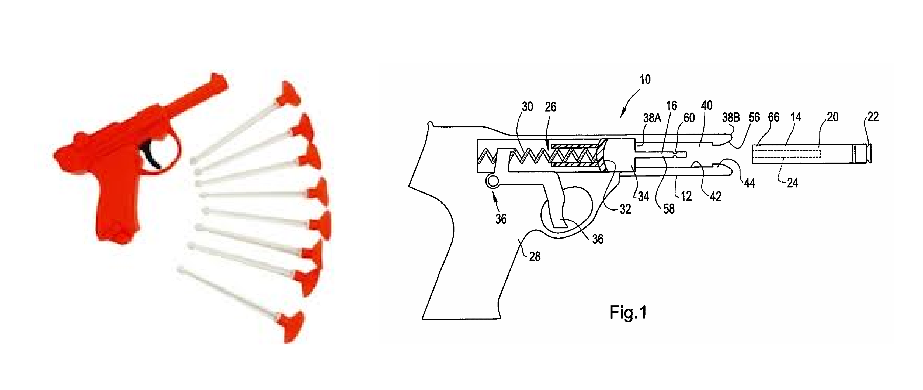
\includegraphics[scale=0.8]{pictures/Spring-design/toy-dart-gun}
  \end{figure}

  \exercise Design an automotive valve spring required to close a valve during combustion. The valve open stroke length should be 5 cm. At its close position, the spring should exert 500 N on the valve. The engine operating speed is between 0 - 6000 rpm.
  \begin{figure}[H]
    \centering
    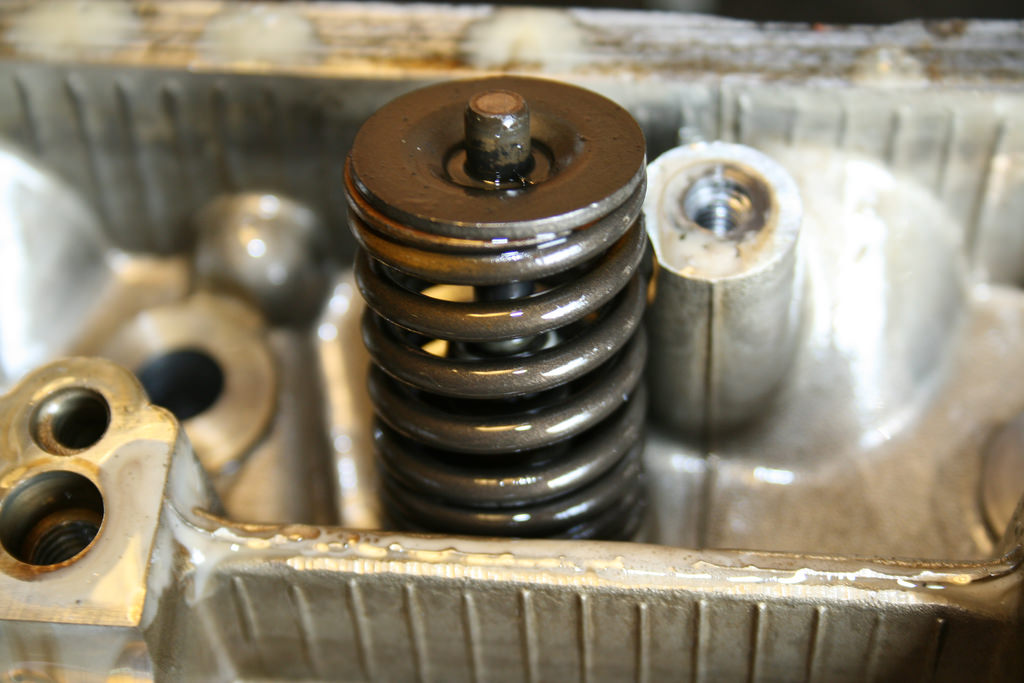
\includegraphics[scale=0.2]{pictures/Spring-design/valve-spring}
  \end{figure}
\end{exercises}

%%%%%%%%%%%%%%%%%%%%%%%%%%%%%%%%%%%%%%%%%%%%%%%%%%%%%%%%%%%%%%%%%%%%%%%%%%%%%%%%%%%%%%%%%%%%%%%%%%%%%%%%%%%%%%%%%%%%%%%%%%%%%%%%%%%%%%%%%%%%%%%%%%%%%%%%%%%%%%%%%%%%%%%%%%%%%%%%%%%%%%%%%%%%%%%%%%%%%%%%%%%%%%%%%%%%%%%%%%%%%%%%%

\part{The Assembly}

%%%%%%%%%%%%%%%%%%%%%%%%%%%%%%%%%%%%%%%%%%%%%%%%%%%%%%%%%%%%%%%%%%%%%%%%%%%%%%%%%%%%%%%%%%%%%%%%%%%%%%%%%%%%%%%%%%%%%%%%%%%%%%%%%%%%%%%%%%%%%%%%%%%%%%%%%%%%%%%%%%%%%%%%%%%%%%%%%%%%%%%%%%%%%%%%%%%%%%%%%%%%%%%%%%%%%%%%%%%%%%%%%

\chapter{Welded Joint Design}

Welding is an addition process whereby two or more components are permanently joined by first partially melting the common surfaces. Once the surfaces cool, the common surface will become more or less homogenous with both materials, thus joining them. It has advantages over other types of joint in that it is typically less expensive and less complicated. It also does not introduce foreign substances to the joint area, nor does it introduce holes and cuts which can lead to stress concentration.

\section{Types of Welding}

Modern industrial welding is done by fusion, with the workpieces melting at their common surfaces. Heat is applied by an electric arc passing between an electrode and the work, by high-amperage electric current passing through the mating workpieces, or by gas flame. Welding takes several forms, typically based on the source of heat, as follows.

\subsection{Electric arc welding}

In this process, workpieces is heated by an electric arc passing from an electrode to the pieces. Electric arc welding is further categorized depending on how the filler material is applied and the way the molten metal is shielded from the atmosphere.

\subsubsection{Shielded metal arc welding (SMAW)}

Also called stick welding, it is the common manual process used for repair work and the welding of large structures. The welder feeds a consumable, coated electrode (welding rod) in the work area. A flux coating on the electrode releases a shielding gas and forms slag around the weld metal. SMAW is typically used with steels.

\begin{figure}[h]
  \centering
  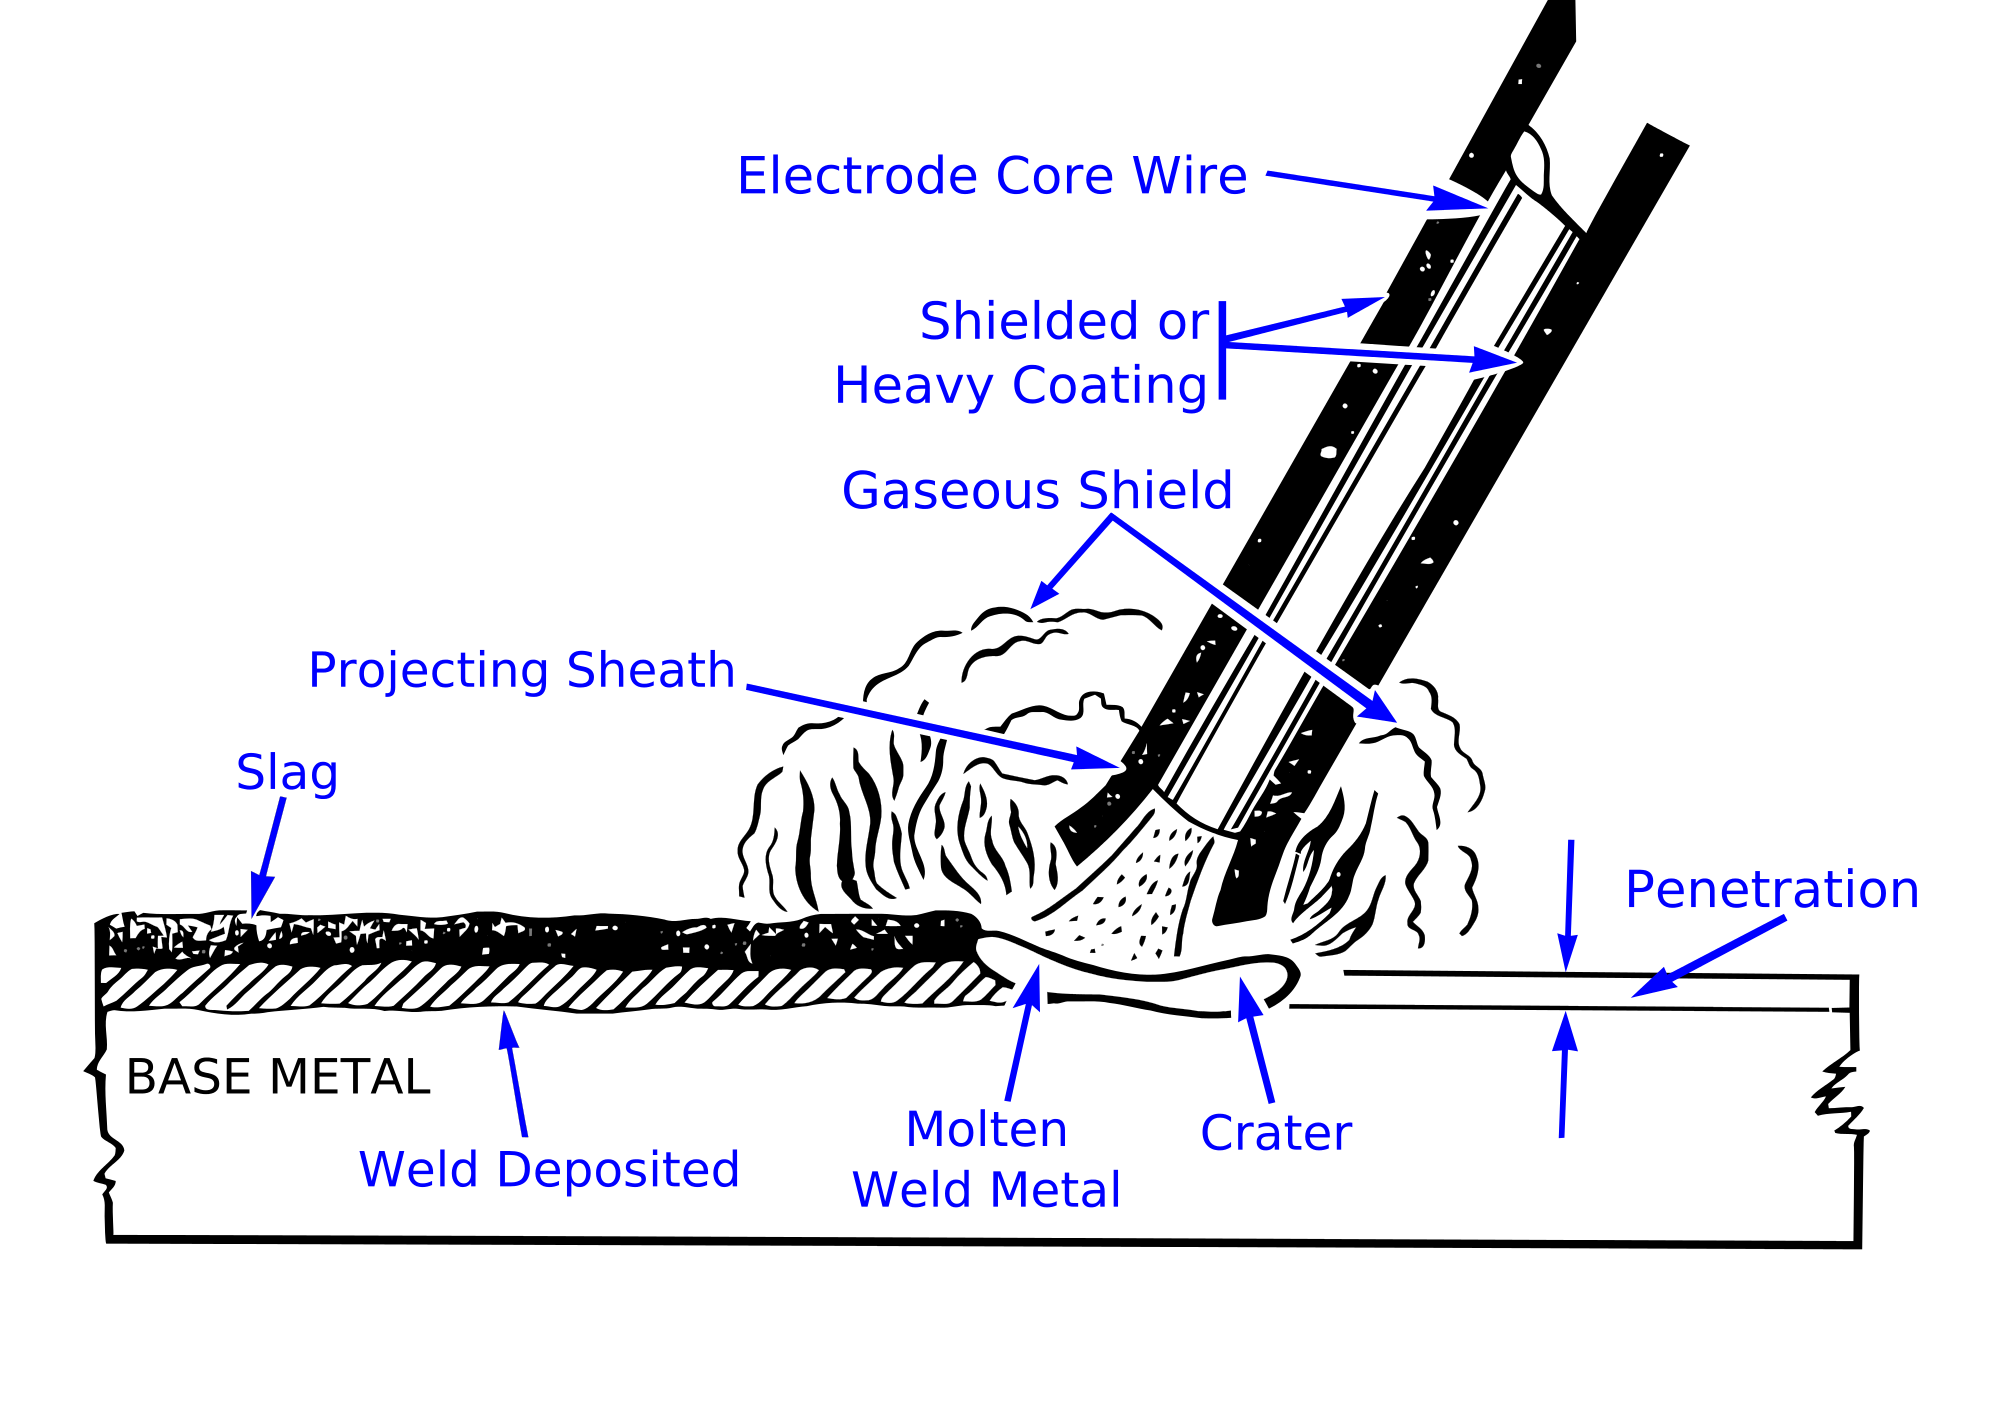
\includegraphics[scale=0.12]{pictures/Welding/shield-metal-arc-welding}
  \caption{Shield metal arc welding (US Army)}
\end{figure}
 
\subsubsection{Gas metal arc welding (GMAW)}

Also called metal-inert gas (MIG) welding, it is a commonly automated process producing high-quality welds at high welding speeds with most metals. The consumable electrode is not coated, but it projects from a nozzle that supplies a shielding gas—argon for aluminum and other non-ferrous metals, low-cost carbon dioxide for steels.

\begin{figure}[h]
  \centering
  \includegraphics[scale=0.1]{pictures/Welding/gas-metal-arc-welding}
  \caption{``A diagram of the GMAW weld area. (1) Direction of travel (2)  Contact tube/electrode wire guide (3) Electrode (4)  Shielding gas (5) Molten weld metal (6) Solidified weld metal (7) Workpiece'' by Nathaniel C. Sheetz is licensed under CC BY-SA 3.0 Unported}
\end{figure}
  
\subsubsection{Gas tungsten arc welding (GTAW)}
Also called tungsten-inert gas (TIG) welding, it employs a nonconsumable tungsten electrode, with a filler wire sometimes fed in separately. A nozzle surrounding the tungsten electrode supplies helium or argon gas for shielding. This process is slower than GMAW but can be used with thinner metals, either ferrous or nonferrous. The process gives high-quality welds of nonferrous and dissimilar metals and can be fully automated.

\begin{figure}[h]
  \centering
  \includegraphics[scale=0.35]{pictures/Welding/gas-tungsten-arc-welding}
  \caption{``Gas tungsten arc welding'' by Duk is licensed under CC BY-SA 3.0 Unported}
\end{figure}
 
\subsubsection{Flux-cored arc welding (FCAW)}

It is much like SMAW, except that the flux is in the hollow core of the consumable electrode rather than on its outer surface. A shielding gas (usually carbon dioxide) is sometimes supplied from a nozzle surrounding the electrode. The process produces fast, clean welds on ferrous metals.

\subsubsection{Submerged arc welding (SAW)}

It is done on flat workpieces. A mound or line of granular flux is deposited on the workpieces in advance of the moving consumable electrode. The flux melts to produce a protective molten slag, under which the fresh weld is “submerged.” The process is commonly used with thick sections requiring deep weld penetration.

\subsection{Resistance Welding}

In this process, electric current generates heat by the process of Joules heating ($I^2R$). The current passes through the workpieces while they are clamped firmly together. No flux or shielding is used, but the process may be carried out in a vacuum or inert gas. Filler material is not typically used. Resistance welding is especially suited for mass production of continuous welds (such as pipe seams) or spot welds of most steels and aluminum alloys. Material thicknesses range from approximately 0.01 – 2 cm.
	
\subsection{Gas welding}

The process is usually performed manually with an oxyacetylene torch and is typically slow. It requires more generalized heating of the work, and is most often used for making repairs. A filler wire is usually, but not necessarily, used.
  
Other kinds of welding processes such as Laser beam, plasma arc, electron beam, and electroslag are also fusion welding and are used on a small scale for very special applications.
Nonfusion, or solid-state welding, processes use a combination of heat and pressure to join parts, though the temperature is usually less than the melting point of the materials.

\section{Welded Joint Strength}

The basic concept of fusion welding is to fuse the materials together into a single and homogenous member. Properties of the welding rod (filler) must be properly matched with those of the parent materials.

Welding electrode material strength and ductility specifications have been standardized by the American Welding Society (AWS). The properties are listed in \cref{table: electrode properties}.

\begin{table}[h]
  \centering
  \caption{Mechanical properties of welding electrodes.}
  \label{table: electrode properties}
    \begin{tabular}{ L{3cm} C{3cm} C{3cm} C{3cm} }
      \toprule
      AWS Electrode Number & Tensile Strength (MPa) & Yield Strength (MPa) & Percent Elongation \\
      \midrule
      E60XX  & 427 & 345 & 17-25 \\
      E70XX  & 482 & 393 & 22 \\
      E80XX  & 551 & 426 & 19 \\
      E90XX  & 620 & 531 & 14-17 \\
      E100XX & 689 & 600 & 13-16 \\
      E120XX & 827 & 737 & 14 \\
      \bottomrule
    \end{tabular}
\end{table}

The American Institute of Steel Construction code provides the suggested permissible stress (and corresponding safety factors) for welded joints.

\begin{table}[h]
  \centering
  \caption{Permissible stresses for weld metal according to AISC code}
  \begin{tabular}{llll}
    \toprule
    Type of Loading & Type of Weld   & Permissible Stress & $N_s$ \\
    \midrule
    Tension         & Butt           & 0.60$S_y$          & 1.67 \\
    Bearing         & Butt           & 0.90$S_y$          & 1.11 \\
    Bending         & Butt           & 0.60 - 0.66$S_y$   & 1.52 - 1.67 \\
    Compression     & Butt           & 0.60$S_y$          & 1.67 \\
    Shear           & Butt or fillet & 0.30$S_{ut}$       & \\
    \bottomrule
  \end{tabular}
\end{table}

\section{Welded Joint Geometry}

Weld geometry depends on the orientation of mating parts. It is one of the two ingredients, along with load direction, in determining the type of stresses exerted on the weld and determining proper weld lengths and effective thicknesses.

\subsection{Butt Welds}
In this type of welded joints, the mating parts are joined by having their ends attached together without any overlap. Typically the ends have the same thickness and length, and after welding, the part essentially become one continuous part. The cross section of the weld is considered to be $H \times L$, even though for most butt welds there are always slight reinforcement so that the thicknesses are slightly larger than $H$.

\begin{figure}[h]
  \centering
  \begin{tikzpicture}[scale=0.8]
    \draw [fill=lightblue] (0,0) --++ (0:5) node(A){} --++ (120:1/cos{30}) node(B){} -- (0,1) -- cycle;
    \draw [fill=LightGrey] (A.center) -- (B.center) arc (120:60:1/cos{30}) node(C){} -- cycle;
    \draw [fill=lightblue] (10,0) node(E){} -- (A.center) -- (C.center) -- (10,1) node(F){} -- cycle;
    \draw [fill=lightblue] (0,1) --++ (45:3) --++ (0:4.42) node(D){} -- (B.center) -- cycle;
    \draw [fill=LightGrey] (B.center) -- (D.center) arc (120:60:1/cos{30}) -- (C.center) arc (60:120:1/cos{30});
    \draw [fill=lightblue, xshift=5.577cm] (0,1) --++ (45:3) --++ (0:4.42) node(G){} --++ (-135:3) -- cycle;
    \draw [fill=lightblue] (E.center) -- (F.center) -- (G.center) --++ (-90:1) -- cycle;
    % dimensioning
    \draw [|<->|] (0,0) ++ (180:0.3) --++ (90:1) node[midway, left]{$H$};
    \draw [|<->|] (B.center) ++ (180:0.5) --++ (45:3) node[midway, left]{$L$};
  \end{tikzpicture}
  \caption{Geometry of a butt weld.}
\end{figure}
 
If the welds are of good quality, they can be considered as strong as the plate, and its efficiency (welded member strength / solid member strength) is 100\%.

\subsection{Fillet Welds}

In this type of welded joint, the weld is formed not on the flat end surface but instead on the angle (typically 90 degree) formed between the mating parts. This type of welds are commonly classified according to the direction of loading: parallel welds or transverse welds.

\begin{figure}[h]
  \centering
  \begin{tikzpicture}[scale=0.8, >=latex]
    \draw [fill=lightblue] (0,0) --++ (0:10) --++ (90:1) node(B){} --++ (180:10) node(A){} node[midway, xshift=-0.4cm](D){} node[midway, xshift=0.4cm](E){} -- cycle;
    \draw [fill=lightblue] (A.center) --++ (45:3) --++ (0:10) node(C){} -- (B.center) -- cycle;
    \draw [fill=lightblue] (B.center) -- (C.center) --++ (-90:1) --++ (-135:3) -- cycle;
    \draw [fill=lightblue] (D.center) --++ (90:5) node(F){} --++ (0:1) node(G){} -- (E.center) --cycle;
    \draw [fill=lightblue] (F.center) --++ (45:3) --++ (0:1) -- (G.center) -- cycle;
    \draw [fill=lightblue] (E.center) -- (G.center) --++ (45:3) --++ (-90:5) -- cycle;
    \draw [fill=LightGrey] (D.center) --++ (90:1) --++ (-1,-1) -- cycle;
    \draw [fill=LightGrey] (E.center) --++ (90:1) node(H){} --++ (1,-1) node(I){} -- cycle;
    \draw [fill=LightGrey] (H.center) --++ (45:3) --++ (1,-1) -- (I.center) -- cycle;
    % dimensioning
    \draw [|<->|] (E.center) ++ (-45:1) --++ (45:0.707) node[midway, above left]{$H$};
    \draw [|<->|] (I.center) ++ (0:1) --++ (45:3) node[midway, above left]{$L$};
  \end{tikzpicture}
  \caption{Geometry of a fillet weld.}
\end{figure}

\section{Welded Joints under Static Axial and Shear Loading} \label{section: stress in weld under axial and shear}

Ideally, if the welding electrode is properly chosen so that it matches the properties of the parent materials, the stress and strength analysis would proceed as though the part were made from a single piece of stock.

The stresses in welds depend both on its geometry and loading direction. In butt welds, the stress in the welds is the same as the stress in the material. Under a normal force $F_n$, the weld is under a normal stress.

\begin{figure}[h]
  \centering
  \begin{tikzpicture}[scale=1.5,>=latex]
    % top left piece
    \draw [fill=lightblue] (0,0) -- ++ (30:2) --++ (150:2) --++ (-150:2) node[midway](C){} --cycle node[midway](A){};
    \draw [fill=LightGrey] (0,0) -- ++ (30:2) --++ (-90:0.5) --++ (-150:2) --cycle;
    \draw [fill=lightblue] (0,0) -- ++ (150:2) --++ (-90:0.5) --++ (-30:2) --cycle;
    % bottom right piece
    \draw [fill=lightblue, xshift=3cm, yshift=-2*0.866cm] (0,0) -- ++ (30:2) node[midway](D){} --++ (150:2) node[midway](B){} --++ (-150:2) --cycle;
    \draw [fill=lightblue, xshift=3cm, yshift=-2*0.866cm] (0,0) -- ++ (30:2) --++ (-90:0.5) --++ (-150:2) --cycle;
    \draw [fill=lightblue, xshift=3cm, yshift=-2*0.866cm] (0,0) -- ++ (150:2) --++ (-90:0.5) --++ (-30:2) --cycle;
    % shear force pair
    \draw[->, very thick] (A.center) --++ (-150:1) node[below left]{$F_s$};
    \draw[->, very thick] (B.center) --++ (30:1) node[above right]{$F_s$};
    % normal force pair
    \draw[->, very thick] (C.center) --++ (150:1) node[above left]{$F_n$};
    \draw[->, very thick] (D.center) --++ (-30:1) node[below right]{$F_n$};
    % surface shear stress
    \foreach \x in {0,...,3} {
      \draw[-right to, thick] (0, -0.125) ++ (30:0.5*\x) --++ (30:0.25);
      \draw[-right to, thick] (0, -0.375) ++ (30:0.5*\x) --++ (30:0.25);
    }
    \draw (0,0) ++ (30:1) node[above left]{$\tau$};
    % surface normal stress
    \foreach \x in {0,...,4}
    \draw[->, thick] (0, -0.25) ++ (30:0.5*\x) --++ (-30:0.5);
    \draw (0,-0.25) ++ (-30:0.5) node[below right]{$\sigma$};
  \end{tikzpicture}
  \caption{Normal and shear stresses on a butt weld cross section under static axial and shear loading.}
\end{figure}

\begin{equation}
  \sigma  = \frac{F_n}{A_w} = \frac{F_n}{HL}
\end{equation}

where $H$ is the throat length and $L$ is the weld length.
Similarly, under a shear force $F_s$, the weld is under a shear stress.

\begin{equation}
  \tau  = \frac{F_s}{A_w} = \frac{F_s}{HL}
\end{equation}

In fillet welds, under parallel loading, both plates exert a shear load on the weld. With transverse loading, one plate exerts a shear load and the other a normal (tensile or compressive) load on the weld. The cross-sectional area size of the weld is defined by the \emph{weld length} and the shortest distance from the intersection of the plates to the straight line connecting the ends of the two legs, also called \emph{throat length} or \emph{effective throat thickness}.

\begin{figure}[h]
  \centering
  \begin{tikzpicture}[>=latex]
    % define nodes
    \path (0,0) ++ (-90:0.5) ++ (-30:0.5) node(E){} ++ (30:2) ++ (150:0.5) ++ (90:0.5) node(F){};
    % bottom right piece
    \draw [fill=lightblue, xshift=1.3cm, yshift=-1.25cm] (0,0) -- ++ (30:2) node[midway](D){} --++ (150:2) node[midway](B){} --++ (-150:2) --cycle;
    \draw [fill=lightblue, xshift=1.3cm, yshift=-1.25cm] (0,0) -- ++ (30:2) --++ (-90:0.5) --++ (-150:2) --cycle;
    \draw [fill=lightblue, xshift=1.3cm, yshift=-1.25cm] (0,0) -- ++ (150:2) --++ (-90:0.5) --++ (-30:2) --cycle;
    % top left piece
    \draw [fill=lightblue] (0,0) -- ++ (30:2cm) --++ (150:2cm) --++ (-150:2) node[midway](C){} --cycle node[midway](A){};
    %\draw [fill=LightGrey] (0,0) -- ++ (30:2) --++ (-90:0.5) --++ (-150:2) --cycle;
    \draw [fill=lightblue] (0,0) -- ++ (150:2) --++ (-90:0.5) --++ (-30:2) --cycle;
    % weld
    \draw [fill=LightGrey] (0,0) -- (E.center) node[midway](G){} --++ (30:2) -- (F.center) --cycle;
    \draw [fill=LightGrey] (0,0) --++ (-90:0.5) -- (E.center) --cycle;
    % shear force pair
    \draw[->, very thick] (A.center) --++ (-150:1) node[below left]{$F_s$};
    \draw[->, very thick] (B.center) --++ (30:1) node[above right]{$F_s$};
    % surface shear stress
    \draw[dashed] (0,0) ++ (-90:0.5) -- (G.center) --++ (30:2);
    \foreach \x in {0,...,3} {
      \draw[right to-, thick, xshift=0.3cm, yshift=-0.1cm] (0, -0.125) ++ (30:0.5*\x) --++ (30:0.25);
      \draw[-right to, thick, xshift=0.4cm] (0, -0.375) ++ (30:0.5*\x) --++ (30:0.25);
    }

    % Axial load in fillet weld
    \node at (7,0) [draw, rectangle, fill=lightblue, minimum height=0.75cm, minimum width=3cm, inner sep=0](M){};
    \node at (M.south east) [anchor=north west,draw, rectangle, fill=lightblue, minimum height=0.75cm, minimum width=3cm, xshift=-1cm](N){};
    % Weld
    \draw [fill=LightGrey](M.north east) -- (M.south east) --++ (0:0.75cm) --cycle;
    \draw [dashed] (M.south east) --++ (45:0.5);
    % Forces
    \draw [->, very thick] (M.west) --++ (180:1) node[left]{$F_n$};
    \draw [->, very thick] (N.east) --++ (0:1) node[right]{$F_n$};
    % Shear stresses
    \draw [right to-, very thick] (M.south east) ++ (0.05,0.15) -- ++ (45:0.3);
    \draw [-right to, very thick] (M.south east) ++ (0.15,0.05) -- ++ (45:0.3);
  \end{tikzpicture}
  \caption{Shear stresses in a fillet weld.}
\end{figure}

The corresponding shear stresses for fillet welds under axial or shear loading is, therefore,

\begin{equation}
  \begin{gathered}
    \tau = \frac{F_s}{HL} \\
    \tau = \frac{F_n}{HL}
  \end{gathered}
\end{equation}

Throat length $H$ should be reasonably proportioned in comparison to the thickness of plates being welded. For practical reasons, $H$ is usually a minimum of 3 mm for plate less than 6 mm thick, and up to a minimum of 15 mm for plates over 150 mm thick. It is also important to note that fillet welds are typically done in pairs to maintain symmetry and avoid any resultant moments, in which case the effective weld area doubles.

\section{Welded Joints under Static Torsional and Bending Loading}

External loading can cause torsional or bending to welded joints when the loads do not pass through the centroid of the welds—also called eccentric loading. If the load is in the plane of the weld group, the welded connection will be subjected to torsion, and if the load is out of plane of the weld group, it will cause bending. Note that there usually are direct loading to the welds caused by these loads as considered in the previous section.

Though a rigorous analysis of each weld segment under torsion or bending is possible, it would be very complicated, involving material properties and geometry of the base materials and the welds. On the other hand, sufficiently accurate results can be obtained by applying the following simplifications.
\begin{enumerate}
\item Direct shear and normal stresses can be assumed uniformly distributed over the length of all welds and calculated as in \cref{section: stress in weld under axial and shear}.
\item The parts being jointed can be assumed rigid and the torsional and bending stresses can be calculated using the conventional formulas.
  
  \[\begin{gathered}
    \tau  = \frac{Tr}{J} \hfill \\
    \sigma  = \frac{My}{I} \hfill \\ 
  \end{gathered} \]

\end{enumerate}

Since the cross section on which the stresses are calculated is the weld group, the corresponding moment of inertia ($I$) and polar moment of inertia ($J$) must be calculated from the weld cross section. In order to determine such moments, we must first locate the centroid of the weld group. The expression for the $x$ and $y$ coordinates of the centroid, $x_c$ and $y_c$ is

\begin{align}
  x_c = \int_A xdA = \sum x_{ci}A_i \\
  y_c = \int_A ydA = \sum y_{ci}A_i
\end{align}

where  $x_{ci}$ and $y_{ci}$ are the $x$ and $y$ coordinates of the centroid of region $i$ and $A_i$ is the area of region $i$. Essentially, they are area-weighted average $x$ and $y$ coordinates.

Given that the centroid of the weld group is at (0,0), and that  the weld cross section has throat length $H$ and weld length $L$, and its centroid is located at ($a, b$), we would have the following moments of inertia

\begin{figure}[h]
  \centering
  \begin{tikzpicture}[scale=0.7, >=latex]
    \draw[fill=lightblue] (3,4) rectangle ++(5,1) node[midway, circle, inner sep=0, fill=black, minimum height=1mm]{} node[midway, xshift=0.5cm] {($a$,$b$)};
    \draw[|<->|] (2.75,4) --++(90:1) node[midway,xshift=-0.5cm]{$H$};
    \draw[|<->|] (3, 3.75) --++ (0:5) node[midway,yshift=-0.5cm]{$L$};
    \draw (0,0) node[midway, circle, inner sep=0, fill=black, minimum height=1mm]{} node[above right]{($x_c$,$y_c$) = (0,0)};
    \draw[<->] (0,-2) --++(90:10) node[above]{$y$};
    \draw[<->] (-2,0) --++(0:10) node[right]{$x$};
  \end{tikzpicture}
\end{figure}

\begin{enumerate}
\item Moments of inertia of a linear weld segment about axes of symmetry through the centroid

  \begin{equation}
    \begin{gathered}
        I_{xc} = \int y^2dA  = 2\int_0^{L/2} y^2Hdy  = \frac{L^3H}{12} \hfill \\
        {I_{yc}} = \frac{H^3L}{12} \hfill \\ 
      \end{gathered}
  \end{equation}
\item Moments of inertia about axes of symmetry through the centroid of the total weld group is equal to the centroidal moments of inertia plus a modification term from the parallel axis theorem.

  \begin{equation}
    \begin{gathered} \label{eqn: weld group moment of inertia}
      I_x = I_{xc} + Ab^2 = \frac{L^3H}{12} + LHb^2 \hfill \\
      I_y = I_{yc} + Aa^2 = \frac{LH^3}{12} + LHa^2 \hfill 
    \end{gathered}
  \end{equation}
\item Polar moment of inertia about an axis perpendicular to the centroid of the weld group.

  \begin{equation}
    J = I_x + I_y = \frac{1}{12}(L^3H + LH^3) + LH(a^2 + b^2)
  \end{equation}
\end{enumerate}

\begin{example} Dual fillet weld on a cantilever beam

  Determine the maximum load $P$ that can be applied to the structure as shown below, given that the safety factor of the weld is 3. The weld has the effective throat thickness of 3 mm, and is made with E70XX series electrode.

  \begin{figure}[H]
    \centering
    \begin{tikzpicture}[>=latex]
      \node at (0,0) [draw, rectangle, inner sep=0, fill=LightBlue, minimum height=0.3cm, minimum width=5cm](A){};
      \node at (A.west) [anchor=east, draw, pattern=north east lines, rectangle, minimum height=2cm, minimum width=1cm]{};
      \draw [fill=LightGrey](A.north west) --++ (90:0.4) -- ++(0.4, -0.4) -- cycle;
      \draw [fill=LightGrey](A.south west) --++ (-90:0.4) -- ++(0.4, 0.4) -- cycle;
      \draw [<-, ultra thick](A.north east) --++ (90:1) node[above]{$P$};
      \node at (A.south west)[yshift=-0.5cm](B){};
      \node at (A.south east)[yshift=-0.5cm](C){};
      \draw [|<->|] (B.center) -- (C.center) node[midway, above]{1 m};
      % welds
      \node at (7,0) [anchor=east, draw, pattern=north east lines, rectangle, minimum height=2cm, minimum width=2cm](D){};
      \node at (D.center)[draw, rectangle, inner sep=0, fill=LightBlue, minimum height=0.3cm, minimum width=2cm](E){};
      \node at (E.north)[draw, anchor=south, rectangle, inner sep=0, fill=LightGrey, minimum height=0.4cm, minimum width=2cm](){};
      \node at (E.south)[draw, anchor=north, rectangle, inner sep=0, fill=LightGrey, minimum height=0.4cm, minimum width=2cm](){};
      % dimensions
      \node at (D.south west)[yshift=-0.5cm](F){};
      \node at (D.south east)[yshift=-0.5cm](G){};
      \draw [|<->|] (F.center) -- (G.center) node[midway, above]{40 cm};
      \draw [|<->|] (A.south east) ++ (0:0.3) --++ (90:0.3) node[midway, right]{12 cm};
    \end{tikzpicture}
  \end{figure}

\end{example}
\begin{solution}

  In this loading configuration, the weld is subjected to shear force and bending moment. The shear force causes shear stress, while the bending moment causes normal stress. First, let us calculate the shear stress, which is

  \[\tau  = \frac{P}{2HL} = \frac{P}{2(0.003)(0.4)} = 417P\]

  Notice the cross sectional area is multiplied by two for the top and bottom welds. The normal bending stress is

  \[\sigma  = \frac{My}{I} = \frac{P(1)(0.06)}{I} = 0.06\frac{P}{I}\]

  The welds’ moment of inertia is given by \cref{eqn: weld group moment of inertia}.

  \[\begin{gathered}
      I_y = 2\left( \frac{LH^3}{12} + LHa^2 \right) \\ 
      = 2\left( \frac{(0.4)(0.003)^3}{12} + (0.4)(0.003)(0.06)^2 \right) \\ 
      = 8.64 \times 10^{-6} \text{ m}^4 \\ 
    \end{gathered} \]

  So the bending stress is

  \[\sigma  = 0.06\frac{P}{8.64 \times 10^{-6}} = 6944P\]

  Since welds can be considered brittle, the maximum normal stress theory will be used to determine failure. The principal stress on the weld is

  \[\begin{gathered}
      \sigma _1 = \frac{6944P}{2} + \sqrt {\left( \frac{6944P}{2} \right)^2 + (417P)^2}  \\ 
      = 6969P \\ 
    \end{gathered} \]

  Finally, we substitute the electrode strength into the safety factor equation to solve for $P$.

  \[\begin{gathered}
      N_s = \frac{\text{strength}}{\text{stress}} \\ 
      3 = \frac{482 \times 10^6}{6969P} \\ 
      P = 23000 \text{ N} \\ 
    \end{gathered} \]

  Note that this is the allowable force considering the weld strength only. The actual allowable force may be less than this, depending on the strength of the beam itself.
\end{solution}

\begin{example}
  Determine the critical point in the welds and its state of stress. The weld throat thickness is 8 mm.

  \begin{figure}[H]
    \centering
    \begin{tikzpicture}
      \node [draw, fill=lightblue, minimum height=5cm, minimum width=5cm](A){};
      \node at (A.east) [anchor=center, draw,  fill=lightblue, minimum height=1.5cm, minimum width=5cm](B){};
      \node at (B.north west) [anchor=south west, draw, fill=LightGrey, minimum height=0.3cm, minimum width=2cm](C){};
      \node at (B.south west) [anchor=north west, draw, fill=LightGrey, minimum height=0.3cm, minimum width=2cm](D){};
      % force
      \draw [->, ultra thick] (B.east) --++ (-90:2) node[below]{20000 N};
      % dimensions
      \draw [|<->|] (C.north west) ++ (90:0.3) --++ (0:2) node[midway, above]{50};
      \draw [|<->|] (D.south west) ++ (-90:0.3) --++ (0:2) node[midway, below]{50};
      \draw [|<->|] (C.south west) ++ (180:0.3) --++ (-90:1.5) node[midway, left]{40};
      \draw [|<->|] (D.south west) ++ (-90:2) --++ (0:5) node[midway, above]{120};
    \end{tikzpicture}
  \end{figure}
\end{example}

\begin{solution}
  Because of the downward load at the end of the beam, the fillet welds are under a combination of shear loading and torsion. In fact, we can (and should) split the problem to analyze the resultant stress from each load and combine those to obtain the final state of stress.

  Let us first tackle the easier of the two problems: shear loading. This is a simple case of a transverse fillet weld (where the shear load is perperndicular to the weld length). The resultant shear stress from shear loading, pointing in the same direction, is
  
  \begin{align*}
    \tau_{shear} &= \frac{P}{2HL} = \frac{20000}{2(0.008)(0.05)} \\
                 &= 25 \text{ MPa}
  \end{align*}

  Now consider the problem of torsion. The applied torque to the weld is the load multiplied with the distance to the center of the welds $L_o$. In this problem the welds are symmetric, thereforce the center is in the middle of the two welds, marked by ...

  The shear stress from torsion can be written as

  \begin{align*}
    \tau_{torsion} &= \frac{Tr}{J_{group}} = \frac{P L_o r_o}{J_{group}} \\
                   &= \frac{20000(0.12-0.05/2) r_o}{J_{group}}
  \end{align*}

  the radius $r_o$ represents the distance away from the center of the weld. With this expression, we know that the shear stress in torsion is the highest at the farthest four corners of the welds, at which points $r_o$ is

  \begin{align*}
    r_o = \sqrt{ \left( \frac{L}{2} \right)^2 + d_o^2 }
  \end{align*}

  where $L$ is the weld length and $d_o$ is the distance from the weld to the center of weld. In this problem $L$ = 5 cm and $d_o$ = 4 cm/2 = 2 cm. Therefore,  

  \begin{align*}
     r_o &= \sqrt{ \left( \frac{0.05}{2} \right)^2 + 0.02^2 } \\
         &= 0.032 \text{ m}
   \end{align*}

   We will also need to calculate the group polar moment of inertia $J_{group}$. It is obvious that neither weld cross sections coincides with the center of weld, so we will need to apply the parallel axis theorem so that

   \begin{align*}
     J_{group} &= J_c + A d_o^2 \\
               &= 2 \left[ \frac{HL^3}{12} +\frac{LH^3}{12} + LHd_o^2 \right] \\
               &= 2 \left[ \frac{(0.008)(0.05)^3}{12} + \frac{(0.05)(0.008)^3}{12} + (0.05)(0.008)(0.02)^2 \right] \\
               &= 1.70 \times 10^{-5} \text{ m}^4
   \end{align*}

   Now we have all the parameters we need, so we can substitute them back into the torsional shear stress equation, which gives

   \begin{align*}
     \tau_{torsion} &= \frac{20000(0.12-0.05/2) r_o}{J_{group}} \\
                    &= \frac{20000(0.095)(0.032)}{1.7 \times 10^{-5}} \\
                    &= 3.58 \text{ MPa}
   \end{align*}

   All four corners have the same magnitude of torsional shear stresses, but their directions differ. The direction of the torsional shear stress is always perpendicular to the vector $r_o$. Therefore, the corner with the maximum combined shear stress (shear + torsional) is corner B and D.

 \begin{figure}[H]
    \centering
    \begin{tikzpicture}
      \node [draw, fill=lightblue, minimum height=5cm, minimum width=5cm](A){};
      \node at (A.east) [anchor=center, draw,  fill=lightblue, minimum height=1.5cm, minimum width=5cm](B){};
      \node at (B.north west) [anchor=south west, draw, fill=LightGrey, minimum height=0.3cm, minimum width=2cm](C){};
      \node at (B.south west) [anchor=north west, draw, fill=LightGrey, minimum height=0.3cm, minimum width=2cm](D){};
      \node at (C.west) [left]{A};
      \node at (C.east) [right]{B};
      \node at (D.west) [left]{C};
      \node at (D.east) [right]{D};
      \draw (C.south) ++ (-90:0.75) node{+} node[above right]{O};
      % force
      \draw [->, ultra thick] (B.east) --++ (-90:2) node[below]{20000 N};
      % stresses
      \draw [->] (C.south east) --++ (-90:1) node[below right]{$\tau_{shear}$};
      \draw [->] (C.south east) --++ (-50:1) node[right]{$\tau_{torsion}$};
      \draw [->] (D.north east) --++ (-130:1) node[right]{$\tau_{torsion}$};
      \draw [->] (D.north west) --++ (130:1) node[right]{$\tau_{torsion}$};
      \draw [->] (C.south west) --++ (50:1) node[right]{$\tau_{torsion}$};
    \end{tikzpicture}
  \end{figure}

  We will consider the state of stress at point B from this point on. The two stresses can then simply be added vectorially, either by breaking them down into $x$ and $y$ components or by using vector addition formula. We will use the latter in this problem.

  \begin{align*}
    \left| \vec{\tau}_{torsion} + \vec{\tau}_{shear} \right|^2 &= \left| \vec{\tau}_{torsion} \right|^2 + \left| \vec{\tau}_{shear} \right|^2 + 2 \vec{\tau}_{torsion} \cdot \vec{\tau}_{shear} \\
                                                               &= \left| \vec{\tau}_{torsion} \right|^2 + \left| \vec{\tau}_{shear} \right|^2 + 2 \left| \vec{\tau}_{torsion} \right| \left| \vec{\tau}_{shear} \right| \cos \alpha
  \end{align*}

  The last piece of the puzzle is to determine the angle $\alpha$ between the two shear stresses. We know that $\tau_{shear}$ is directly downward while $\tau_{torsion}$ is perpendicular to vector OB. Thus,

  \begin{align*}
    \tan \alpha &= \frac{d_o}{L/2} = \frac{2 d_o}{L} \\
                &= \frac{2(0.02)}{0.05} = 0.8 \\
    \alpha &= \tan^{-1} 0.8 = 38.7^{\circ}
  \end{align*}

  Substitute $\alpha$ into the vector addition formula to obtain the combined shear stress

  \begin{align*}
    \left| \vec{\tau}_{torsion} + \vec{\tau}_{shear} \right|^2 &= 25^2 + 3.58^2 + 2(25)(3.58) \cos 38.7^{\circ} \\
                                                               &= 778 \\
    \left| \vec{\tau}_{torsion} + \vec{\tau}_{shear} \right| &= \left| \vec{\tau}_{total} \right| = 27.9 \text{ MPa}                                                        
  \end{align*}
  
\end{solution}

\section{Asymmetric Welded Joints}

There may arise situations where weld joints need not, or cannot, be symmetrical. This is mostly due to the geometry of the joining parts. In such cases, the same methodology applied to design of symmetrical joints is still applicable, but we must be cautious and do not assume any symmetry in the direction or magnitude of a stress or load. Since the welds are not symmetric, the center of weld will likely not be in the ``middle.'' As such, critical point analysis must be done more carefully.

\begin{example}
  The weld dimensions and load are given in the figure.
  \begin{center}
    \includegraphics[scale=0.55]{pictures/Welding/weld-under-torsion-and-bending}
  \end{center}
  If the weld throat thickness is 5 mm using E60 series, Determine this weld safety factor.
\end{example}

\begin{solution}
  The problem is similar to the previous torsion problem. The only difference being the weld is asymmetric. Center of weld ($G$) must be determined mathematically, and that is our first task.
  
  Using the equation for center of weld and setting the origin (0,0) at $B$, we have
  
  \begin{align*}
    x_G &= \frac{(0.15H)(0) + (0.1H)(0.05)}{ 0.15H + 0.1H } \\
        &= 0.02 \text{ m} \\
    y_G &= \frac{(0.15H)(-0.075) + (0.1H)(0)}{ 0.15H + 0.1H } \\
        &= -0.045 \text{ m} 
  \end{align*}

  The problem can be split into a pure shear load problem and a pure torsion problem. Let us first tackle the former.
  
  The shear stress from shear load is simply
  
  \begin{align*}
    \tau_{shear} &= \frac{P}{H(L_1 + L_2)} \\
                 &= \frac{20000}{0.005(0.10 + 0.15)} \\
                 &= 16 \text{ MPa}
  \end{align*}

  Onto the pure torsion problem. Here, the formula for shear stress from torsion still applies

  \begin{align*}
    \tau_{torsion} &= \frac{P L_o r_o}{J_{group}} \\
                   &= \frac{20000(0.3 - 0.02)r_o}{J_{group}} \\
  \end{align*}

  Unfortunately, the asymmetric weld complicates the problem in two ways.
  \begin{enumerate}
  \item Center of weld is not in the middle, the modification term in parallel axis theorem for $J_{group}$ must take the distance between the center of weld and each weld's centroid.
  \item Center of weld is not in the middle $\rightarrow$ $r_o$ is different for each corner of the weld, making it difficult to locate the critical point.
  \end{enumerate}

  Let us first calculate $J_{group}$

  \begin{align*}
    J_{group} &= J_c + A d_o^2 \\
              &= \frac{H(L_1^3 + L_2^3)}{12} +\frac{(L_1 + L_2)H^3}{12} + H(L_1d_{Gc1}^2 + L_2d_{Gc2}^2)
  \end{align*}

  where $d_{Gc1}$ and $d_{Gc2}$ are the distances from center of weld $G$ to the centroid of weld 1 and 2, respectively.

  \begin{align*}
    d_{Gc1}^2 &= (0.02-0)^2+(0.075-0.045)^2 \\
              &= 1.3 \times 10^{-3} \\
    d_{Gc2}^2 &= (0.05-0.02)^2 + (0.045 - 0)^2 \\
              &= 2.93 \times 10^{-3}
  \end{align*}

  Substitute the values to find $J_{group}$
  \begin{align*}
    J_{group} &= \frac{(0.005)(0.1^3 + 0.15^3)}{12} +\frac{(0.1 + 0.15)(0.005)^3}{12} \\
              &+ (0.005)(0.1(1.3 \times 10^{-3}) + 0.15(2.93 \times 10^{-3})) \\
              &= 4.27 \times 10^{-6} \text{ m}^4
  \end{align*}

  Now, to address the critical point. We know that the direction of $\tau_{torsion}$ at each spot will be perpendicular to the vector $r_G$ connecting the center of weld to that point.

  \begin{center}
    \begin{tikzpicture}
      \node {\includegraphics[scale=0.6]{pictures/Welding/weld-under-torsion-and-bending}};
      \node at (-2.5,0.5) (G){};
      \draw[->] (G.center) --++ (1.67,0.92) node(A){};
      \draw[->] (A.center) --++ (-60:1) node[below]{$\tau_{torsionA}$};
      \draw[->] (G.center) --++ (-0.4,-2.25) node(C){};
      \draw[->] (C.center) --++ (165:1.2) node[left]{$\tau_{torsionC}$};
      \draw[->] (G.center) --++ (-0.4,1) node(B){};
      \draw[->] (B.center) --++ (25:0.7) node[right]{$\tau_{torsionB}$};
    \end{tikzpicture}
  \end{center}
  
  From the figure, it should be obvious that the resultant stress at B is definitely not the highest since its $\tau_{torsionB}$ is the smallest out of all the points. Furthermore, the $y$-component of $\tau_{torsionB}$ is opposite to $\tau_{shear}$. Only A and C are possible candidates for critical points now. We will first proceed to calculate $\tau_{torsionA}$.

  \begin{align*}
    \tau_{torsionA} &= \frac{P L_o r_{GA}}{J_{group}} \\
                    &=\frac{20000(0.28) r_{GA}}{4.27 \times 10^{-6}} \\[1em]
    r_{GA} &= \sqrt{(0.1 - 0.02)^2 + 0.045^2} \\
                    &= 0.092 \text{ m} \\[1em]
    \tau_{torsionA} &= 121 \text{ MPa}
  \end{align*}

  Combine $\tau_{shear}$ and $\tau_{torsionA}$, we have
  \begin{align*}
    \cos \alpha &=  \frac{0.08}{0.092} = 0.87 \\
    \tau_{total} &= \sqrt{ 16^2 + 121^2 + 2(16)(121) \cos 29.4^{\circ} } \\
           &= 135 \text{ MPa} \\[1em]
  \end{align*}
  
  Let us now consider $\tau_{torsionC}$
  \begin{align*}
    \tau_{torsionA} &= \frac{P L_o r_{GC}}{J_{group}} \\
                    &=\frac{20000(0.28) r_{GC}}{4.27 \times 10^{-6}} \\[1em]
    r_{GC} &= \sqrt{(0.15 - 0.045)^2 + 0.02^2} \\
                    &= 0.107 \text{ m} \\[1em]
    \tau_{torsionA} &= 140 \text{ MPa}
  \end{align*}

  Combine $\tau_{shear}$ and $\tau_{torsionC}$, we have
  \begin{align*}
    \beta &= 90^{\circ} + \cos^{-1} \frac{0.105}{0.107} \\
          &= 101.1^{\circ} \\[1em]
    \tau_{total} &= \sqrt{ 16^2 + 140^2 + 2(16)(140) \cos 101.1^{\circ} } \\
          &= 137 \text{ MPa} \\[1em]
  \end{align*}

  The resultant shear stress at $C$ is larger, hence $C$ is the critical point. So the safety factor of this weld is
  \begin{align*}  
    N_s &= \frac{427}{135} = 3.12
  \end{align*}
\end{solution}


\section{Fatigue Considerations in Welded Joints}

When welded joints are subjected to fatigue loading, small voids and inclusions which have little effect on static strength can constitute local stress concentration and reduce fatigue strength. In addition, the weld material extending beyond the plane of the plates—reinforcement—can cause stress concentration at the edges of the weld bead. In fact, to increase fatigue strength, the weld bead should be ground to flush with the plates. Approximate fatigue stress concentration factors associated with butt weld reinforcement and other weld geometries are given in \cref{table: fatigue stress concentration factor}.
\begin{table}[h]
  \centering
  \caption{Approximate fatigue stress concentration factors of different weld joints, $K_f$.}
  \label{table: fatigue stress concentration factor}
    \begin{tabular}{ L{10cm} C{2cm} }
      \toprule
      Type of Weld & $K_f$ \\
      \midrule
      Butt weld, reinforcement intact, tensile load & 1.2 \\
      Toe of fillet weld, transverse loading & 1.5 \\
      End of fillet weld, parallel loading & 2.7 \\
      T-butt joint weld, with sharp corners, tensile loading & 2.0 \\
      \bottomrule
  \end{tabular}
\end{table}

\begin{example} Fatigue analysis of a butt weld

  A butt weld is subjected to a repeated axial load $F$ ranging from 50000 to 100000 N as shown. The thickness of the material is 0.5 cm. The joint is welded with E60 series electrode. Determine the proper weld length if the required safety factor is 3.

  \begin{figure}[H]
    \centering
    \includegraphics[scale=0.7]{pictures/Welding/fatigue-weld-analysis-example}
  \end{figure}
\end{example}
\begin{solution}
  Based on Soderberg relation, we have that

  \[\frac{\sigma _a}{S_e} + \frac{\sigma _m}{S_y} = \frac{1}{N_s}\]

  We can simply calculate the amplitude and average stresses.

  \[\begin{gathered}
      \sigma_m = \frac{100000 + 50000}{2HL} = \frac{75000}{0.5 \times 10^{-2}L} = \frac{1.5 \times 10^7}{L} \hfill \\
      \sigma_a = \frac{100000 - 50000}{2HL} = \frac{25000}{0.5 \times 10^{-2}L} = \frac{5 \times 10^6}{L} \hfill \\ 
    \end{gathered} \]

  However, due to stress concentration from reinforced butt weld, the actual average stress and stress amplitudes are

  \[\begin{gathered}
      \sigma_m = 1.2\left( \frac{1.5 \times 10^7}{L} \right) = \frac{1.8 \times 10^7}{L} \hfill \\
      \sigma_a = 1.2\left( \frac{5 \times 10^6}{L} \right) = \frac{6 \times 10^6}{L} \hfill \\ 
    \end{gathered} \]

  The yield strength and endurance limit for E60 series are 345 MPa and $0.45 \times 427 = 192$ MPa, respectively. Substituting the values into Soderberg relation, we have

  \[\begin{gathered}
      \frac{\sigma_a}{S_e} + \frac{\sigma_m}{S_y} = \frac{1}{N_s} \hfill \\
      {1 \over L} \left( \frac{6 \times 10^6}{192 \times 10^6} + \frac{1.8 \times 10^7}{345 \times 10^6} \right) = \frac{1}{3} \hfill \\
      L = 2.5 \times {10^{-1}} = 25\text{ cm} \hfill \\ 
    \end{gathered} \]
\end{solution}

\section*{Summary}

In this chapter, load and stress analyses of welds are given in details. Strengths and weaknesses of different types of available welding processes are discussed. Geometry of the joint is possibly the most important in analyzing and properly designing weld joints. In fact, the analyses of welded joints are similar to their solid member counter parts, the only difference being taking into account changes in moments of inertia. Additional factors involved static vs. fatigue loading. Two key design parameters involved are the electrodes and the geometry of the weld (length and effective throat thickness).

\section*{Exercises}

\begin{exercises}
  \exercise Short answers
  \begin{enumerate}
  \item Why are most fillet welds done in pairs and not singles?
  \item Explain the differences between arc welding and resistance welding?
  \item Why is gas welding mainly used in maintenance but not in manufacturing?
  \end{enumerate}
  \exercise A springboard is welded to the wall as shown below. The springboard length is 3 m and has a constant cross-section of a 5 cm x 30 cm rectangle. The welds are arranged as shown, using E80xx series electrode with the effective throat thickness of 5 mm. The springboard is made of AISI1040 having $E$ = 210 GPa and yield strength = 300 MPa. Determine the maximum weight of a swimmer that the springboard can support. Note that the safety factors of the weld and the springboard are 4 and 2, respectively.
  \begin{figure}[H]
    \centering
    \includegraphics[scale=0.7]{pictures/Welding/springboard-exercise}
  \end{figure}
  \exercise Determine the maximum allowable load P that can be applied on the free end of this welded cantilever beam. The electrode used is E80xx series and the effective throat thickness of all welds is 5 mm. Other dimensions are given below. The safety factor of this welded joint is 3.
  \begin{figure}[H]
    \centering
    \includegraphics[scale=0.72]{pictures/Welding/parallel-weld-exercise}
  \end{figure}
\end{exercises}


%%%%%%%%%%%%%%%%%%%%%%%%%%%%%%%%%%%%%%%%%%%%%%%%%%%%%%%%%%%%%%%%%%%%%%%%%%%%%%%%%%%%%%%%%%%%%%%%%%%%%%%%%%%%%%%%%%%%%%%%%%%%%%%%%%%%%%%%%%%%%%%%%%%%%%%%%%%%%%%%%%%%%%%%%%%%%%%%%%%%%%%%%%%%%%%%%%%%%%%%%%%%%%%%%%%%%%%%%%%%%%%%%


\chapter{Bolted Joint Design}

At first look, threaded fasteners seem to be the most mundane of machine elements. Upon further investigation, one can see that these seemingly simple components exist in amazing variety and designs. Economically, they contribute to substantial sum of any project especially structural and large fabricating ones. The safety implications for these fasteners used are obvious. Many fasteners must be designed for easy and low-cost assembly while others must be designed for ease of disassembly. There are also some that must be difficult to remove.

In this chapter, various guidelines and considerations involved in the design and selection of proper threaded fasteners are discussed. Applications of threaded fasteners in simple joints are also illustrated.

\section{Thread forms, terminology, and standards}

The basic arrangement of a helical thread wound around a cylinder are illustrated in \cref{fig: bolt terms}. Pitch, lead, and lead angle are defined by the illustrations. Virtually all bolts and screws have a single thread, but power screws sometimes have double, triple, or even quadruple threads.

\begin{figure}[h]
  \centering
  \includegraphics[scale=1.1]{pictures/Bolt/bolt-terminology}
  \caption{Terminology of screw threads.}
  \label{fig: bolt terms}
\end{figure}

\Cref{fig: bolt terms} shows the standard geometry of screw threads used on fasteners. This is essentially the same for both \emph{Unified} (inch series) and \emph{ISO} (metric) threads. Standard sizes for the two systems given in \cref{table: ISO Screw Dimensions} show both the \emph{fine thread} (UNF, Unified National Fine) and \emph{coarse thread} (UNC, Unified National Coarse) series. The pitch diameter, $d_p$, is the diameter of a cylinder on a perfect thread where the width of the thread and groove are equal. The \emph{stress area} tabulated is based on the average of the pitch and root diameters. This is the area used for stress (force/area) calculations. Note: Metric threads are identified by diameter and pitch as M10 $\times$ 1.5
\begin{table}[h]
  \centering
  \caption{Basic Dimensions of ISO Metric Screw Threads.}
  \label{table: ISO Screw Dimensions}
    \begin{tabular}{ L{2cm} C{1.5cm} C{1.5cm} C{1.5cm} C{1.5cm} C{1.5cm} C{1.5cm} }
      \toprule
      \multirow{2}{3cm}{Nominal Diameter $d$} & \multicolumn{3}{c}{Coarse Threads} & \multicolumn{3}{c}{Fine Threads} \\ \cmidrule{2-7}
      & Pitch & Minor Dia & Stress Area & Pitch & Minor Dia & Stress Area \\
      \midrule
      3 & 0.5 & 2.39 & 5.03 & - & - & - \\
      3.5 & 0.6 & 2.76 & 6.78 & - & - & - \\
      4 & 0.7 & 3.14 & 8.78 & - & - & - \\
      5 & 0.8 & 4.02 & 14.2 & - & - & - \\
      6 & 1 & 4.77 & 20.1 & - & - & - \\
      7 & 1 & 5.77 & 28.9 & - & - & - \\
      8 & 1.25 & 6.47 & 36.6 & 1 & 6.77 & 39.2 \\
      10 & 1.5 & 8.16 & 58.0 & 1.25 & 8.47 & 61.2 \\
      12 & 1.75 & 9.85 & 84.3 & 1.25 & 10.5 & 92.1 \\
      14 & 2 & 11.6 & 115 & 1.5 & 12.2 & 125 \\
      16 & 2 & 13.6 & 157 & 1.5 & 14.2 & 167 \\
      18 & 2.5 & 14.9 & 192 & 1.5 & 16.2 & 216 \\
      20 & 2.5 & 16.9 & 245 & 1.5 & 18.2 & 272 \\
      22 & 2.5 & 18.9 & 303 & 1.5 & 20.2 & 333 \\
      24 & 3 & 20.3 & 353 & 2 & 21.6 & 384 \\
      27 & 3 & 23.3 & 459 & 2 & 24.6 & 496 \\
      30 & 3.5 & 25.7 & 561 & 2 & 27.6 & 621 \\
      33 & 3.5 & 28.7 & 694 & 2 & 30.6 & 761 \\
      36 & 4 & 31.1 & 817 & 3 & 32.3 & 865 \\
      39 & 4 & 34.1 & 976 & 3 & 35.3 & 1030 \\
      42 & 4.5 & 36.9 & 1121 & - & - & - \\
      48 & 5 & 42.7 & 1473 & - & - & - \\
      \bottomrule
  \end{tabular}
\end{table}

Coarse-threaded bolts are more resistant to cross-threading and thread stripping. They tend to be less susceptible to damage and require less assembly time.

Fine-threaded bolts, on the other hand, are less prone to loosen under vibration. The threads are easier to tap, especially on high-strength materials. Also, because of their fine threads, allow for finer adjustment and require less torque to obtain the same preload.

\section{Static Screw Stresses}

When in use, screws are subjected to various stresses such as torsion during tightening, axial load, and thread bearing stresses. Let us consider each type of stress separately.

\subsection{Torsion}

Threaded fasteners are subjected to torsional stresses during tightening, much like a cylindrical bar being twisted. The shear stress caused by the exerted torque is
\[\tau  = \frac{Tc}{J} = \frac{16T}{\pi d_r^3}\]
where $d_r$ is the thread root diameter.
With threaded fasteners, the equivalent of substantial collar friction is normally present, in which case it is customary to assume that the torque transmitted through the threaded section is approximately half the wrench torque.

\subsection{Axial Load}

The main purpose of threaded fasteners is to hold work pieces together by exerting compressive forces on them. Therefore they are typically subjected to tensile loads. The effective area for threaded fasteners is the tensile area $A_t$.

The distribution of the axial stress near the ends of the loaded portion of a screw is not uniform. This is not a concern for static loading because threaded fasteners should always have enough ductility to permit local yielding at thread roots without damage. However, when we consider fatigue loading of bolts, this stress concentration is very important.

\subsection{Combined Torsion and Axial Load}

The combination of the stresses can be treated with multiaxial stress analysis which has been covered in \cref{section: multiaxial stress} using maximum distortion energy theory or maximum shear stress theory since bolts and screws are considered ductile. With threaded fasteners, it is normal for some yielding to occur at the thread roots during initial tightening.

\subsection{Thread Bearing (Compressive) Stress}

\Cref{fig: force flow in bolt} illustrates the force flow through a bolt and a nut used to clamp two members together. Compression between the screw and nut threads exists on all threads. This type of direct compression is typically called bearing, and the area used for stress calculation is the projected area which for each thread is $\pi(d_2 - d_i^2) / 4$. The number of threads in contact is seen from the figure to be $t/p$. Thus, the bearing stress on each thread is

\begin{figure}[h]
  \centering
  \includegraphics[scale=0.5]{pictures/Bolt/force-flow-bolt}
%  \begin{tikzpicture}
%    \draw[decorate,thick,decoration={screw, screw radius=70pt, thread amplitude=20pt, thread separation=30pt, head length=0pt}] (0,7) -- (0,-0.5);
%    \draw[->, very thick] (-1.5,7)  node[yshift=0.5cm, xshift=0.5cm,rotate=-90]{$\Bigg\{$} node[yshift=1cm, xshift=0.5cm]{Total = $P$} to [out=-120,in=45] (-2.5,6) to [in=0,out=-135](-4,5.5) to [out=180,in=-90](-4.5,7);
%    \draw[->, very thick] (-1,7) to [out=-100,in=45] (-2.5,3.8) to [in=0,out=-135](-4,3.3) to [out=180,in=-90](-5,7);
%    \draw[->, very thick] (-0.5,7) to [out=-90,in=45] (-2.5,1.6) to [in=0,out=-135](-4,1.1) to [out=180,in=-90](-5.5,7) node[yshift=0.5cm, xshift=0.5cm,rotate=-90]{$\Bigg\{$} node[yshift=1cm, xshift=0.5cm]{Total = $P$};
%  \end{tikzpicture}
  \caption{Force flow in a bolt in tension \cite{juvinall2006fundamentals}}
  \label{fig: force flow in bolt}
\end{figure}

\begin{equation}
  \sigma  = \frac{4P}{\pi (d^2 - d_r^2)}\frac{p}{t}
\end{equation}

It is important to note that this equation only gives an average value of the stress. In fact, the stress is not uniformly distributed among the threads because of factors such as bending of the threads and manufacturing variations. Furthermore, the threads all share the same load, similar to members of a compound bar, the load will be distributed most to the shortest (and stiffest) path. Hence, threads which are closer to the clamped members will carry higher loads and stresses.

\subsection{Thread Shear (Stripping) Stress and Nut Thickness
  Requirement}

Nut or bolt threads can be stripped along its cylindrical surface under sufficient overload. From the thread geometry shown in \cref{fig: force flow in bolt} the shear area is equal to $\pi d(0.75t)$, where $d$ is the diameter of the shear fracture surface involved.

Now, assume that both the nut and bolt are made of the same material, the nut thickness required to balance the bolt tensile strength and thread stripping strength can be calculated. First the bolt tensile force required to yield the threaded cross section is

\[F_{bolt} = A_tS_y \approx \frac{\pi}{4}(0.9d)^2S_y\]

where $d$ is the major diameter of the thread. On the other hand, the bolt tensile load required to yield the thread-stripping failure surface of the nut based on a parabolic stress distribution is

\[F_{nut} = \pi d(0.75t)S_{sy} \approx \pi d(0.75t)(0.58S_y)\]

where $t$ is the nut thickness. Equating $F_{bolt}$ and $F_{nut}$ to balance the bolt and nut strengths gives

\begin{figure}[h]
  \centering
  \begin{tikzpicture}
    \draw[decorate,thick,decoration={screw, screw radius=0.65cm, thread amplitude=2pt, thread separation=3pt, head width=2.0cm, head length=0.5cm}] (0,5) -- (0,-1);
    % clamped members
    \draw[fill=LightBlue] (-3,0.5) rectangle (-0.8,2.5);
    \draw[fill=LightBlue, xshift=3.8cm] (-3,0.5) rectangle (-0.8,2.5);
    \draw[fill=LightGrey] (-3,2.5) rectangle (-0.8,4.5);
    \draw[fill=LightGrey, xshift=3.8cm] (-3,2.5) rectangle (-0.8,4.5);
    % nut
    \draw[fill=Grey!30] (-1.5,0) rectangle (-0.75,0.5);
    \draw[fill=Grey!30] (0.75,0) rectangle (1.5,0.5);
    \draw[fill=Grey!50] (-0.75,0) rectangle (0.75,0.5);
    % dimensioning
    \draw[|<->|] (-0.7,-1.5) --++ (0:1.4) node[midway, yshift=-0.3cm]{$d$};
    \draw[|<->|] (2, 0) --++ (90:0.5) node[midway,xshift=0.3cm]{$t$};
  \end{tikzpicture}
\end{figure}

\begin{equation} \label{eqn: required nut thickness}
  t = 0.47d
\end{equation}

Since the nuts are usually softer than bolts in order to allow slight yielding of the top threads and more uniform load distribution among the threads, the standard nut thickness is approximately $7d/8$.

\section{Thread Fastener Types}

\Cref{fig: threaded fasterner types} shows basic types of threaded fasteners. Screws and bolts are by far the most common types, and the difference between them is only one of intended use. Bolts are intended for use with nuts; screw are intended for screwing into tapped holes.

\begin{figure}[h]
  \centering
  \begin{tikzpicture}
    % clamped members
    \node at (0,-0.5) [anchor=south,draw, rectangle, fill=lightblue, minimum width=2.8cm, minimum height=2cm](A){};
    \node at (A.north west) [anchor=south west,draw, rectangle, fill=lightblue, minimum width=1cm, minimum height=1cm]{};
    \node at (A.north east) [anchor=south east,draw, rectangle, fill=lightblue, minimum width=1cm, minimum height=1cm]{};
    % bolt
    \draw[decorate,thick,decoration={screw, screw radius=0.3cm, thread amplitude=1pt, thread separation=2pt, head width=1.0cm, head length=0.5cm}] (0,3) -- (0,0);
    % description
    \node at (0,-1) {(a) Screw};
     % bolt
    \draw[decorate,thick,decoration={screw, screw radius=0.3cm, thread amplitude=1pt, thread separation=2pt, head width=1.0cm, head length=0.5cm}] (4,3) -- (4,-0.25);
    % clamped members
    \node at (2.6,0.5) [anchor=south west,draw, rectangle, fill=lightblue, minimum width=1cm, minimum height=1cm](A){};
    \node at (A.south east) [anchor=south west,draw, rectangle, fill=lightblue, minimum width=1cm, minimum height=1cm, xshift=0.75cm](B){};
    \node at (A.north) [anchor=south,draw, rectangle, fill=lightblue, minimum width=1cm, minimum height=1cm]{};
    \node at (B.north) [anchor=south,draw, rectangle, fill=lightblue, minimum width=1cm, minimum height=1cm]{};
    % nut
    \node at (4,0) [anchor=south, draw, rectangle, fill=Grey!50, minimum height=0.5cm, minimum width=0.5cm](C){};
    \node at (C.east) [anchor=west, draw, rectangle, fill=Grey!70, minimum height=0.5cm, minimum width=0.3cm]{};
    \node at (C.west) [anchor=east, draw, rectangle, fill=Grey!30, minimum height=0.5cm, minimum width=0.3cm]{};
    % description
    \node at (4,-1) {(b) Bolt and nut};
    % clamped members
    \node at (8,-0.5) [anchor=south,draw, rectangle, fill=lightblue, minimum width=2.8cm, minimum height=2cm](D){};
    \node at (D.north west) [anchor=south west,draw, rectangle, fill=lightblue, minimum width=1cm, minimum height=1cm]{};
    \node at (D.north east) [anchor=south east,draw, rectangle, fill=lightblue, minimum width=1cm, minimum height=1cm]{};
    % bolt
    \draw[decorate,thick,decoration={screw, screw radius=0.3cm, thread amplitude=1pt, thread separation=2pt, head width=0cm, head length=0cm}] (8,3.25) -- (8,0);
    % nut
    \node at (8,2.5) [anchor=south, draw, rectangle, fill=Grey!50, minimum height=0.5cm, minimum width=0.5cm](E){};
    \node at (E.east) [anchor=west, draw, rectangle, fill=Grey!70, minimum height=0.5cm, minimum width=0.3cm]{};
    \node at (E.west) [anchor=east, draw, rectangle, fill=Grey!30, minimum height=0.5cm, minimum width=0.3cm]{};
    % description
    \node at (8,-1) {(c) Stud and nut};
     % bolt
    \draw[decorate,thick,decoration={screw, screw radius=0.3cm, thread amplitude=1pt, thread separation=2pt, head width=0cm, head length=0cm}] (12,3.25) -- (12,-0.25);
    % clamped members
    \node at (10.6,0.5) [anchor=south west,draw, rectangle, fill=lightblue, minimum width=1cm, minimum height=1cm](F){};
    \node at (F.south east) [anchor=south west,draw, rectangle, fill=lightblue, minimum width=1cm, minimum height=1cm, xshift=0.75cm](G){};
    \node at (F.north) [anchor=south,draw, rectangle, fill=lightblue, minimum width=1cm, minimum height=1cm]{};
    \node at (G.north) [anchor=south,draw, rectangle, fill=lightblue, minimum width=1cm, minimum height=1cm]{};
    % bottom nut
    \node at (12,0) [anchor=south, draw, rectangle, fill=Grey!50, minimum height=0.5cm, minimum width=0.5cm](H){};
    \node at (H.east) [anchor=west, draw, rectangle, fill=Grey!70, minimum height=0.5cm, minimum width=0.3cm]{};
    \node at (H.west) [anchor=east, draw, rectangle, fill=Grey!30, minimum height=0.5cm, minimum width=0.3cm]{};
    % top nut
    \node at (12,2.5) [anchor=south, draw, rectangle, fill=Grey!50, minimum height=0.5cm, minimum width=0.5cm](I){};
    \node at (I.east) [anchor=west, draw, rectangle, fill=Grey!70, minimum height=0.5cm, minimum width=0.3cm]{};
    \node at (I.west) [anchor=east, draw, rectangle, fill=Grey!30, minimum height=0.5cm, minimum width=0.3cm]{};
    % description
    \node at (12,-1) {(d) Threaded rod};
  \end{tikzpicture}
  \caption{Bolted joint applications.}
  \label{fig: threaded fasterner types}
\end{figure}

A stud is threaded on both ends and is usually screwed permanently into a tapped hole. Threads on the two ends may or may not be identical. A threaded rod is the least common type. It is usually used when a very long threaded member is desired. A threaded rod can often be purchased in lengths of a few feet and then cut off as required.

  \begin{figure}[h]
    \centering
    \includegraphics[width=\textwidth]{pictures/Bolt/head-types}
    \caption{Various screw and bolt head types. (Alma Bolt Company)}
    \label{fig: head types}
  \end{figure}

   \begin{figure}[h]
    \centering
    \includegraphics[width=0.9\textwidth]{pictures/Bolt/drive-types}
    \caption{Various screw and bolt drive types. (Unknown)}
  \end{figure}

\Cref{fig: head types} shows most of the common fastener head styles and drive types. As a rule, a bolt can also serve as a screw by using it with a tapped hole. Hexagonal-head screws and bolts are commonly used for connecting machine components. Sometimes they cannot be used because of insufficient clearance to put a socket or wrench on the head. In such cases the hexagonal-socket head is often used.

\section{Fastener Materials and Methods of Manufacture}

Materials for screws, nuts, and bolts are normally selected based on strength, weight, corrosion resistance, magnetic properties, life expectancy, and cost. Most fasteners are made from steel of specifications standardized by the Society of Automotive Engineers and summarized in \cref{table: SAE grade properties}.
\begin{table}[h]
  \centering
  \caption{Specifications for steel used in millimeter series screws and bolts.}
  \label{table: SAE grade properties}
  \begin{tabular}{ l C{1.8cm} C{1.8cm} C{1.8cm} C{1.8cm} C{1.8cm} C{1.8cm} }
    \toprule
    SAE Class & Diameter $d$ (mm) & Proof Strength $S_p$ (MPa) & Yield Strength $S_y$ (MPa) & Tensile Strength $S_{ut}$ (MPa) & Elongation (\%) & Reduction of Area (\%) \\
    \midrule
    4.6 & 5 – 36 & 225 & 240 & 400 & 22 & 35 \\
    4.8 & 1.6 – 16 & 310 & - & 420 & - & - \\
    5.8 & 5 – 24 & 380 & - & 520 & - & - \\
    8.8 & 17 – 36 & 600 & 660 & 830 & 12 & 12 \\
    9.8 & 1.6 – 16 & 650 & - & 900 & - & - \\
    10.9 & 6 – 36 & 830 & 940 & 1040 & 9 & 9 \\
    12.9 & 1.6 – 36 & 970 & 1100 & 1220 & 8 & 8 \\
    \bottomrule
  \end{tabular}
\end{table}

Heading is typically done cold for diameters up to 2 cm and heated for larger sizes. Threads are usually formed by rolling between dies that force the material to cold-form into the threaded contour of the die grooves. Threads formed this way are stronger than cut or ground threads in fatigue and impact loading because cold working can leave compressive residual stresses at the thread roots (see . Because of these advantages, high-strength screws and bolts should have rolled threads. Furthermore, the greatest fatigue strength is obtained if the threads are rolled after heat treatment so that the resulting work hardening and favorable residual stresses are not lost.

\begin{figure}[h]
  \centering
  \includegraphics[width=0.5\textwidth]{pictures/Bolt/thread-rolling}
  \caption{Process of thread rolling. (Profiroll Technologies)}
\end{figure}

\begin{figure}[h]
  \centering
  \includegraphics[width=0.5\textwidth]{pictures/Bolt/thread-cutting}
  \caption{Process of thread cutting. (CustomPartNet)}
\end{figure}

\begin{figure}[h]
  \centering
  \includegraphics[width=0.8\textwidth]{pictures/Bolt/cut-rolled-thread}
  \caption{Compressive residual stress at the root of rolled thread.}
\end{figure}

Fasteners are also made from aluminum, brass, copper, nickel, stainless steel, titanium, and various plastics. Fastener materials must always be considered in connection with any potential corrosion problems associated with the environment and the other metals involved. Additionally, appropriate coatings should be considered for corrosion protection and to reduce thread friction and wear.

\section{Bolt Tightening and Initial Tension}

For most applications, screws and nut-bolt assemblies should ideally be tightened to produce an initial tensile force $F_i$ nearly equal to the full “proof load,” which is defined as the maximum tensile force that does not produce a normally measurable permanent set. On this basis, initial tensions are commonly specified in accordance with the equation

\[F_i = K_iA_tS_p\]

where At is the tensile stress area of the thread, Sp is the proof strength of the material, and Ki is a constant, usually specified in the range of 0.75 to 1.0. For ordinary applications involving static loading, $K_i \approx 0.9$ or

\begin{equation}
  F_i = 0.9A_tS_p
\end{equation}

\Cref{fig: bolt mohr circles} illustrates bolt stress, both initially when tightening torque is still applied and finally after the tightening torque is removed. The stress element shown is in the shank.

\begin{figure}[h]
  \centering
  \begin{tikzpicture}
    % cylinder
    \node (0,0) [fill=SkyBlue,cylinder, shape border rotate=180,draw, minimum height=7cm, minimum width=2cm]{};
    % element
    \draw (-0.3,-0.3) rectangle (0.3,0.3);
    % stresses on element
    \draw [->] (-0.3,0) --++ (180:0.5) node[left]{$\sigma$};
    \draw [->] (0.3,0) --++ (0:0.5) node[right]{$\sigma$};
    \draw [-right to] (0.3,0.4) --++ (180:0.6) node[midway, yshift=2mm]{$\tau$};
    \draw [-right to] (-0.3,-0.4) --++ (0:0.6) node[midway, yshift=-2mm]{$\tau$};
    \draw [-left to] (-0.4,-0.3) --++ (90:0.6);
    \draw [-left to] (0.4,0.3) --++ (-90:0.6);   
    % Mohr circles
    \draw[xshift=6cm, fill=SkyBlue] circle(1.5cm);
    \draw[xshift=6cm, fill=White] circle(1.3cm);
    \draw[<->] (4.7,-2) --++(90:4);
    \draw[<->] (4,0) --++(0:4);
    \draw[fill] (4.7,0) circle(1.5pt)  node[below left, xshift=-1mm]{(0,0)} ;
    \draw (4.7,0.75) node[circle,fill,inner sep=1.5pt]{} node[left]{(0,$\tau$)} --++ (-30:3) node[circle,fill,inner sep=1.5pt]{} node[right]{($\sigma$,$-\tau$)} --++(90:0.75) node[circle,fill,inner sep=1.5pt]{} node[above right, xshift=1mm]{$(\sigma$,0)};
  \end{tikzpicture}
  \caption{Mohr circles of the states of stress at the shank of a bolt during and after tightening.}
  \label{fig: bolt mohr circles}
\end{figure}

An analysis of forces, torque, and thread geometry is required to derive the relationship between the tightening torque and initial tension in a screw.
Turning a screw can be considered an equivalent to pushing an object up an inclined plane. By unwinding one turn of the screw thread, a geometrical relationship between the lead, lead angle, and diameter is

\begin{equation}
  \tan \lambda  = \frac{L}{\pi d_m}
\end{equation}

A segment of the nut or threaded material is represented in Figure … by the small block acted upon by load $w$ (a portion of the total axial load $W$), normal force $n$, friction force $f$, and tangential force $t$. Note that force $t$ times $d_m/2$ represents the torque applied to the nut segment.

Summing tangential forces acting on the block gives

\begin{equation} \label{eqn: sum bolt tangent force}
  q - n(f\cos \lambda  + \cos \alpha_n\sin \lambda ) = 0
\end{equation}

Summing axial forces gives

\begin{equation} \label{eqn: sum bolt axial force}
  w + n(f\sin \lambda  - \cos \alpha_n\cos \lambda ) = 0
\end{equation}

Combining \cref{eqn: sum bolt tangent force} and \cref{eqn: sum bolt axial force} gives

\[q = w\frac{f\cos \lambda + \cos \alpha_n\sin \lambda }{\cos \alpha_n\cos \lambda  - f\sin \lambda }\]

Since the small block represents a typical segment of nut thread, integration over the entire thread surface in contact results in the same equations except the forces are now the $total$ tangential, vertical, and normal loads. The equation for torque required to create tensile force $W$ is

\begin{equation}
  T = Q\frac{d_m}{2} = \frac{Wd_m}{2}\frac{f\cos \lambda + \cos \alpha_n\sin \lambda }{\cos \alpha_n\cos \lambda - f\sin \lambda }
\end{equation}

The lead $L$ rather than the lead angle $\lambda$ is usually a known standard value, a more convenient form of the torque equation is obtained by dividing the numerator and denominator by $\cos \lambda$ and then substituting $L/\pi d_m$ for $\tan \lambda$. This gives

\[T = \frac{Wd_m}{2}\frac{f\pi d_m + L\cos \alpha_n}{\pi d_m\cos \alpha_n - fL}\]

If the coefficient of friction of the washer is $f_c$, then the added torque required to overcome collar friction is $Wf_cd_c/2$, and the total torque required to create tensile force $W$ is

\begin{equation} \label{eqn: required bolt tightening torque}
  T = \frac{Wd_m}{2}\frac{f\pi d_m + L\cos \alpha_n}{\pi d_m\cos \alpha_n - fL} + \frac{Wf_cd_c}{2}
\end{equation}

The analysis for torque required to remove the bolt is the same except that the directions of applied tangential force $q$ and friction $f$ are reversed. The total torque required to remove the bolt with tension $W$ is

\[T = \frac{Wd_m}{2}\frac{f\pi d_m - L\cos \alpha_n}{\pi d_m\cos \alpha_n + fL} + \frac{Wf_cd_c}{2}\]

An equation relating tightening torque to initial tension can be obtained from \cref{eqn: required bolt tightening torque} by substituting the both coefficients of friction with 0.15 as a rough estimate. For standard screw threads, we have

\begin{equation}
  T = 0.2F_id
\end{equation}

where $d$ is the nominal major diameter of the thread.

\section{Thread Loosening and Thread Locking}

An inherent advantage of threaded fasteners in comparison with riveting or welding is that they can be easily disassembled without destroying the joints. A disadvantage is that they sometimes loosen and disassemble themselves.
Under static conditions, a self-locking screw is one that requires a positive torque to lower then load, and an overhauling screw is one that has low enough friction to enable the load to lower itself. If collar friction can be neglected, \cref{eqn: thread locking} for $T \geqslant 0$ shows that a screw is self-locking if

\begin{equation} \label{eqn: thread locking}
  f \geqslant \frac{L\cos \alpha_n}{\pi d_m}
\end{equation}

It is important to note that a self-locking screw under static conditions may still loosen when exposed to vibration as the screw seeks to relax its initial tension. The following factors can influence thread loosening

\begin{enumerate}
\item Helix angle: larger helix angles allow for higher tendency of loosening. Therefore, coarse threads tend to loosen more easily than fine threads.
\item Initial tightening: greater initial tightening leads to larger frictional force the must be overcome when loosening.
\item Clamping surfaces: Soft or rough clamping surfaces can promote plastic deformation which decreases the initial tension and promotes loosening.
\item Surface conditions: Surface treatments and conditions that increases the friction coefficient provide increased resistance to loosening.
\end{enumerate}
  
In fact, the problem of thread loosening has resulted in numerous and ingenious special designs and modifications. Some common solutions to the problem include

\begin{enumerate}
\item Helical and toothed lock washers. They work on the principle of biting into the mating metal surfaces and resist loosening by a wedging action.
\item Slotted or castle nuts are used with a cotter pin or wire that fits in diametrically opposite slots and passes through a drilled hole in the bolt. This provides a positive lock but may require a slight overtightening or undertightening in order to align a pair of slots with the bolt hole.
\item Locknuts. There are generally two types—free-spinning and prevailing torque. The free-spinning locknuts spin on freely until seated and the produce a deflection when tightened that causes a gripping of the mating bolt threads. The prevailing-torque locknuts develop a friction torque as soon as the threads are fully engaged. They require wrenching to the final seated position and have a strong tendency to stay in position even when not tightened. Prevailing-torque nuts or fasteners usually provide the best solution in critical applications, particularly when extreme vibration is involved.
\item Two standard nuts. Sometimes they can be used together to obtain a locking action. The extra standard nut or is installed first and tighten gently. Then the standard nut is installed and fully tightened against the extra nut.
\end{enumerate}

\section{Bolt Tension and Bolted Joint Stiffness}

Bolts are typically used to hold parts together in opposition to forces pulling or sliding them apart. Understanding load distribution between the bolt and clamped parts is key to evaluating strength of a bolted joint.

Upon tightening, the bolt starts to exert compressive load on the clamped parts, and in the process the clamped parts exert tensile load on the bolt. After initial tightening, the bolt is going to be in under a tensile load $F_i$ while the clamped parts are under an equal compressive load. This load $F_i$ is called the \emph{preload}.

In an event where there is an external axial load applied to the joint, both the bolt and the clamped parts undergo axial deformation depending on the load distributed between the two. One method of analyzing load distribution in a bolted joint is to consider it as a compound bar. Similar to a bolted joint, a compound bar is made of multiple materials connected together in parallel, undergoing identical longitudinal deformation. Recalling the formula for load distribution in a 2-member compound bar, we have

\begin{equation} \label{eqn: 2-member compound bar}
  P_i = P_{ext}\frac{\dfrac{E_iA_i}{L_i}}{\dfrac{E_1A_1}{L_1} + \dfrac{E_2A_2}{L_2}}
\end{equation}

where $P_i$ is the load distributed in the ith member of the bar and $P$ is the axial load applied on the compound bar. Looking back at Hooke’s law, the term $EA/L$ in fact represents the stiffness in axially loaded member, for example,

\[\begin{gathered}
  \delta  = \frac{FL}{AE} = \frac{F}{k} \hfill \\
  k = \frac{EA}{L} \hfill \\ 
\end{gathered} \]

Rewriting \cref{eqn: 2-member compound bar} using stiffnesses of the bolt $k_b$ and of the clamped parts $k_j$, the new expression becomes

\begin{figure}[h]
  \centering
  \begin{tikzpicture}[scale=1]
    \draw[decorate,line width=0pt,Black!50!Grey,decoration={screw, screw radius=0.6cm, thread amplitude=2pt, thread separation=3pt, head width=2.5cm, head length=0.8cm}] (0,5) -- (0,-1);
    % clamped members
    \draw[fill=LightBlue] (-3,0.5) rectangle (-0.8,2.3);
    \draw[fill=LightBlue, xshift=3.8cm] (-3,0.5) rectangle (-0.8,2.3);
    \draw[fill=LightBlue] (-3,2.3) rectangle (-0.8,4.2);
    \draw[fill=LightBlue, xshift=3.8cm] (-3,2.3) rectangle (-0.8,4.2);
    % springs
    \draw[decoration={aspect=0.2, segment length=9mm, amplitude=1.5cm,coil},decorate, line width=8pt, Blue!60] (0,4.2) -- (0,0) node(A){} node[midway, xshift=-1.8cm]{$k_j$};
    \draw[decoration={aspect=0.2, segment length=6mm, amplitude=0.6cm,coil},decorate, ultra thick] (0,4.2) --  (0,0) node[midway,black, xshift=1cm]{$k_b$};
    % nut
    \node at (0,-0.5) [anchor=south, draw, rectangle, fill=Grey!50, minimum height=1cm, minimum width=1cm](B){};
    \node at (B.east) [anchor=west, draw, rectangle, fill=Grey!70, minimum height=1cm, minimum width=0.7cm]{};
    \node at (B.west) [anchor=east, draw, rectangle, fill=Grey!30, minimum height=1cm, minimum width=0.7cm]{};
  \end{tikzpicture}
  \caption{A bolted joint stiffness represented by two springs in parallel. The inner coil represents the bolt stiffness, while the other represents the clamped part stiffness.}
\end{figure}

\begin{equation}
  P_b = P\frac{k_b}{k_b + k_j}
\end{equation}

This shows that the amount of external load distributed in the bolt and clamped parts depends on their stiffness. The total loads carried in the bolt and clamped parts are simply

\begin{figure}[h]
  \centering
  \begin{tikzpicture}[scale=0.8]
    \draw [->] (0,0) node(A){} node[below right]{bolt extension $\rightarrow$} --++ (90:6) node[above]{$F_b$};
    \draw (0,0) --++ (0:10);
    \draw [->, xshift=10cm] (0,0) node(B){} node[below left]{$\leftarrow$ joint compression} --++ (90:6) node[above]{$F_j$};
    \draw [SkyBlue!50!Blue, very thick](A.center) --++ (30:8) node(C){} node(F)[above, black,yshift=0.5cm]{$P=0$} -- (B.center);
    \draw [SkyBlue!50!Blue, dashed] (C.center) --++ (30:1.5) node(D){} --++ (-90:2.3) node(E){};
    \draw [|<->|] (D.east) -- (E.east) node[midway, right]{$P>0$};
    \draw [dashed] (C) -- ++ (180:7) node[left]{$F_i$};
    \draw [->] (C) -- (F);
  \end{tikzpicture}
  \caption{Forces in bolt and clamped parts with and without external applied force $P$.}
  \label{fig: bolt-joint interaction}
\end{figure}

\begin{align} \label{eqn: bolt-joint interaction}
  F_b &= P_b + F_i = CP + F_i \\
  F_j &= (1 - C)P - F_i
\end{align}

where $C = k_b/(k_b + k_j)$.

\Cref{fig: bolt-joint interaction} graphically represents the bolt-clamped-parts interaction. When there is no external load ($P$ = 0), there bolt and the clamped parts carry equal and opposite load $F_i$. When there is external load, the fraction of the load distributed depend on their stiffnesses and simply add (or subtract) from the original preload $F_i$.

\subsection{Bolt Stiffness}

The bolt stiffness $k_b$ comes from the stifnesses of both the threaded ($k_t$ and unthreaded ($k_u$) parts that are engaged within the thickness of the joint. The two parts are connected in series, hence the bolt stiffness can be calculated using a formula for stiffness of two serially connected members.

\begin{align}
  \frac{1}{k_b} &= \frac{1}{k_u} + \frac{1}{k_{t}} \nonumber \\ 
  \frac{1}{k_b} &= \frac{L_u}{EA_u} + \frac{L_{t}}{EA_{t}} \nonumber \\ 
  k_b &= E\left( \frac{A_uA_{t}}{L_uA_{t} + L_{t}A_u} \right) 
\end{align}

For simplicity, the root diameter is assumed to be 0.9 times the major diameter. If the bolt is threaded all the way through, the expression for bolt stiffness reduces to

\begin{align}
  k_b = \frac{EA_t}{L} \approx \frac{\pi (0.9d)^2 E}{4L} \approx \frac{0.64d^2E}{L}  \label{eqn: bolt stiffness}
\end{align}

\subsection{Clamped Parts Stiffness}

Similar to bolt stiffness, the stiffness of clamped parts is analogous to two (or more) serially connected springs. Let us consider two clamped materials whose individual stiffnesses are $k_1$ and $k_2$, respectively. Their combined stiffness is

\begin{align}
  \frac{1}{k_j} &= \frac{1}{k_1} + \frac{1}{k_2} \nonumber \\ 
  \frac{1}{k_j} &= \frac{L_1}{E_1A_1} + \frac{L_2}{E_2A_2}
\end{align}

The same analogy can be applied for $n$ parts clamped together, so that

\begin{align}
  \frac{1}{k_j} &= \frac{1}{k_1} + \frac{1}{k_2} + ... + \frac{1}{k_n} \nonumber \\ 
  \frac{1}{k_j} &= \frac{L_1}{E_1A_1} + \frac{L_2}{E_2A_2}+ ... + \frac{L_n}{E_nA_n} 
\end{align}

The effective cross-sectional area of the clamped parts can be difficult to determine. In many cases, the effective area can be approximate by drawing a cone 30-degree from the bolt head and nut outward and calculate its average value throughout the clamped part thickness. The bolt head diameter is approximately 1.5 times the major diameter of the bolt. So the effective cross-sectional area of clamped parts, $A_c$ can be expressed as

\begin{figure}[h]
  \centering
  \begin{tikzpicture}[>=latex]
    \draw[decorate,thick,decoration={screw, screw radius=0.65cm, thread amplitude=2pt, thread separation=4pt, head width=2.5cm, head length=0.8cm}] (0,5) -- (0,-1);
    % clamped members
    \draw[fill=LightBlue] (-3,0.5) rectangle (-0.8,2.3);
    \draw[fill=LightBlue, xshift=3.8cm] (-3,0.5) rectangle (-0.8,2.3);
    \draw[fill=LightGrey] (-3,2.3) rectangle (-0.8,4.2);
    \draw[fill=LightGrey, xshift=3.8cm] (-3,2.3) rectangle (-0.8,4.2);
    % nut
    \draw[fill=Grey!30] (-1.5,0) rectangle (-0.75,0.5);
    \draw[fill=Grey!30] (0.75,0) rectangle (1.5,0.5);
    \draw[fill=Grey!50] (-0.75,0) rectangle (0.75,0.5);
    % dimensioning
    \draw[|<->|] (-0.7,-1.4) --++ (0:1.4) node[midway, yshift=-0.3cm]{$d_1 = d$};
    \draw[|<->|] (2, 0) --++ (90:0.5) node[midway,xshift=0.3cm]{$t$};
    \draw[|<->|] (-1.25, 5.3) --++ (0:2.5) node[midway,yshift=0.3cm]{$d_2 = 1.5 d$};
    % 30-degree cone
    \draw[dashed]  (-1.5,0.5) --++ (120:1.9);
    \draw[dashed]  (1.5,0.5) --++ (60:1.9);
    \draw[dashed]  (-1.25,4.2) --++ (-120:2.5);
    \draw[dashed]  (1.25,4.2) --++ (-60:2.5);
  \end{tikzpicture}
  \caption{Effective area for calculating clamped part stiffness.}
\end{figure}

\begin{align}
  A_c = \frac{\pi}{4} \left[ \left( \frac{d_3 + d_2}{2} \right)^2 - d_1^2 \right] \label{eqn: clamped parts area}
\end{align}

where 

\begin{align*}
  d_1 &= d \\
  d_2 &= 1.5d \text{ for standard hexagonal-headed bolts} \\
  d_3 &= d_2 + L \tan 30^{\circ} 
\end{align*}

Substitute these value in \cref{eqn: clamped parts area} gives

\begin{align}
  A_c &= \frac{\pi}{16}(5d^2 + 6dL \tan 30^{\circ} + L^2 \tan^2 30^{\circ}) \nonumber \\
      &\approx d^2 + 0.68dL + 0.065L^2 \label{eqn: clamped parts area approx}
\end{align}

In many bolted joints, the two (or more) clamped parts are made of the same material. In such cases, the clamped part stiffness can be written as

\begin{align}
  k_j = \frac{EA_c}{L_1+L_2}
\end{align}

\begin{example} Determine the stiffness ratio $C$ for a bolted joint made of two 1-cm thick aluminum plates held together by an M8 bolt and nut. $E_{Al}$ = 70 GPa and $E_{steel}$ = 210 GPa.
\end{example}

\begin{solution}
  First, start by determining the bolt stiffness. An M8 bolt obviously has the diameter of 8 mm. We will assume that the bolt is threaded all the way through. Utilizing \cref{eqn: bolt stiffness}, we have

  \begin{align*}
    k_b &= \frac{0.64d^2E}{L} \\
        &= \frac{0.64 (0.008^2)(210 \times 10^9)}{0.01+0.01} \\
        &= 4.3 \times 10^8 \text{ N/m}
  \end{align*}
  
  To evaluate the clamped parts stiffness, we must determine their effective cross-sectional area first. Using \cref{eqn: clamped parts area approx}, we have that

  \begin{align*}
    A_c &\approx d^2 + 0.68dL + 0.065L^2 \\
        &= 0.008^2 + 0.68(0.008)(0.02) + 0.065(0.02)^2 \\
        &= 1.99 \times 10^{-4} \text{ m}^2
  \end{align*}

  We can then determine the clamped parts stiffness.

  \begin{align*}
    k_j &= \frac{E_{Al}A_c}{L} \\
        &= \frac{70 \times 10^9 \times 1.99 \times 10^{-4}}{0.02} \\
        &= 6.97 \times 10^8 \text{ N/m}
  \end{align*}

  Finally, the stiffness ratio $C$ is

  \begin{align*}
    C & = \frac{k_b}{k_b + k_j} = \frac{4.3}{4.3 + 6.97} \\
      &= 0.38
  \end{align*}

  Note that $C$ in this example is larger than normal because the clamped material (aluminum) is softer than the bolt (steel). In this case, it may be advisable to use a washer to increase $A_c$ and to increase the clamped parts stiffness.
\end{solution}


\section{Bolt Selection for Static Loading}

The primary loading applied to bolts is tensile, shear, or a combination of the two. There may be some bending when the clamped parts are not parallel or not perpendicular to the bolt axis. Before considering more sophisticated examples, it is important to recognize that screws and bolts are sometimes chosen arbitrarily. This is true for most noncritical applications where loads are small in which case bolt size selection is simply a matter of judgment and ease of assembly.

\subsection{Tension Joints}

The primary application of bolted joints is to exert compressive load on clamped parts, thus preventing them from coming apart under external tensile loads. In tension joints, the preload in the bolts directly combat the external tensile loads.

From the bolt-joint stiffness interaction \cref{eqn: bolt-joint interaction}, it is clear that preload plays a crucial role in maintaining the integrity of a bolted joint. By keeping the clamped parts intact, the bolted joint distribute a small fraction of external load to the bolt, while the main bulk of the load is carried by the clamped parts. If ever the clamping force in the clamped parts become positive (no longer compressive), the joint would separate. The bolt will have to carry the entire external load, which usually breaks the bolt.

With that understanding, the required clamping force (and thus bolt size) when an external tensile load $P$ is applied can be determined by making sure that the clamping force remains compressive (less than zero) with the applied external load. Let us explore the external force that leads to zero clamping load.

\[\begin{gathered}
  F_j = 0 = (1 - C)P - F_i \\ 
  P = \frac{F_i}{1 - C} \\ 
\end{gathered} \]

For non-permanent joints, the general guideline is that the preload should approximately be 75\% of the bolt’s proof load.

\[P = \frac{0.75F_p}{1 - C} = \frac{0.75S_pA_t}{1 - C}\]

For general bolt joint designs, it is safe to assume that the stiffness ratio $C$ is close to 0.25

\[\begin{gathered}
  P = \frac{0.75S_pA_t}{1 - 0.25} = S_pA_t \\ 
  A_t = \frac{P}{S_p} \\ 
\end{gathered} \]

For the bolted joint to have a safety factor of $N_s$

\begin{equation} \label{eqn: tension joint bolt sizing}
  A_t = \frac{N_sP}{S_p}
\end{equation}

\subsection{Friction Joints}

Another application for bolted joints is to prevent clamped parts from sliding apart under shear forces. It is a common misconception that bolted joints can prevent such sliding by the interference of bolts or screws, as in the case of pins. Bolted joints rely friction between the parts to prevent them from sliding. The only contribution bolts makes to friction joints is the preload which increases friction between clamped parts. Therefore, the maximum shear force capacity $P_{shear}$ of a friction joint is

\begin{figure}[h]
  \centering
  \begin{tikzpicture}[>=latex]
    \draw[decorate,thick,decoration={screw, screw radius=0.65cm, thread amplitude=2pt, thread separation=4pt, head width=2.5cm, head length=0.8cm}] (0,5) -- (0,-1);
    % clamped members
    \draw[fill=LightBlue] (-3,0.5) rectangle (-0.8,2.3);
    \draw[fill=LightBlue, xshift=3.8cm] (-3,0.5) rectangle (-0.8,2.3);
    \draw[fill=LightGrey] (-3,2.3) rectangle (-0.8,4.2);
    \draw[fill=LightGrey, xshift=3.8cm] (-3,2.3) rectangle (-0.8,4.2);
    % nut
    \draw[fill=Grey!30] (-1.5,0) rectangle (-0.75,0.5);
    \draw[fill=Grey!30] (0.75,0) rectangle (1.5,0.5);
    \draw[fill=Grey!50] (-0.75,0) rectangle (0.75,0.5);
    % forces
    \draw[->, ultra thick] (-2,2.3) --++ (-90:2) node (A){} node[right]{$F_i$};
    \draw[->, ultra thick] (A.west) --++ (90:0.8) node (B){} node[midway,left]{$P(1-C)$};
    \draw[<-, ultra thick, Blue]  (B.center) --++ (90:1.2) node[midway,left]{$F_j$};
    \draw[->, line width=3pt] (-3,3.3) --++ (180:2) node[left]{$P_{shear}$};
    \draw[->, line width=3pt] (3,1.4) --++ (0:2) node[right]{$P_{shear}$};
  \end{tikzpicture}
  \caption{Forces in a typical friction joint.}
\end{figure}

\[P_{shear} = -\mu F_j\]

where $\mu$ is the coefficient of friction between clamped parts and $F_j$ is the clamping force on the parts. The negative sign is there to correct the sign: friction is generated only when clamping force is compressive ($F_j < 0$), and for later calculation it is more convenient if friction comes out positive.

Typically, when the friction joint is not also loaded in tensile direction, the clamping force is equal to the preload. However, when the joint is loaded in the tensile direction, the clamping force is changed. Taking the same assumptions for tension joints (preload is approximately 75\% of proof load and stiffness ratio is 0.25), the expression for shear force capacity of the joint is 

\begin{align*}
  P_{shear} &= -\mu F_j = -\mu \left( P(1 - C) - F_i \right) \\
            &= \mu (0.75S_pA_t - 0.75P)
\end{align*}

For the friction joint to have a safety factor of $N_s$, the potential friction force generated by the bolted joint must be Ns times the external shear force.

\begin{equation}
  N_s = \frac{\mu F_j}{P_{shear}} = \frac{0.75\mu (S_pA_t - P)}{P_{shear}}
\end{equation}

Therefore, the required tensile area of the bolt is

\begin{equation}
  A_t = \frac{\dfrac{N_s P_{shear}}{0.75\mu } + P}{S_p}
\end{equation}

Upon closer inspection of the equation, the required tensile area is simply the sum of the areas for a friction joint without external load $P$ and tension joint under load $P$.

\begin{equation}
  A_t = \frac{N_s P_{shear}}{0.75\mu S_p } + \frac{P}{S_p}
\end{equation}

\begin{example}
  An bracket is attached to a wall with a bolts. The bracket, during operation, will be subjected to a load as shown in the figure. Determine the required bolt size if the safety factor of the joint is 2 and the coefficient of friction between the bracket and the wall is 0.5.

  \centering
  \begin{tikzpicture}
    \node [draw, rectangle, minimum height=3cm, minimum width=1cm, pattern=north east lines](A){};
    \node at (A.east) [anchor=west, draw, rectangle, minimum height=1cm, minimum width=0.3cm, fill=lightblue](B){};
    \node at (B.center) [draw, rectangle, minimum height=0.3cm, minimum width=0.6cm, fill=black](C){};
    \draw [<-](C.north east) --++ (45:1) node[above]{bolt};
    \draw [->, ultra thick] (B.south east) --++ (-60:1.5) node[right]{2000 N};
    \draw [dashed, thin] (B.south east) --++ (-90:1.4) node[right]{$30^{\circ}$};
  \end{tikzpicture}
\end{example}
\begin{solution}
  In this problem, the load applies both a tensile and shear loads onto the joint. We must consider bolt sizing equations for both tension and friction joints to determine the proper answer.

  Let us first consider the joint as a tension joint, the horizontal component of the 2000-N load is one applying the tensile load. If we pick material SAE grade 4.8 for our bolts, the proper sizing is

  \begin{align*}
    A_t &= \frac{N_s P}{S_p} \\
        &= \frac{(2)(2000 \sin 30^{\circ})}{225 \times 10^6} \\
        &= 8.89 \times 10^{-6} \text{ m}^2 = 8.89 \text{ mm}^2
  \end{align*}

  Looking back at \cref{table: ISO Screw Dimensions}, this calls for an M5$\times$0.8 bolt.

  Now, let us consider the joint as a friction joint, the vertical component is the shearing load, and the horizontal component is the tensile load, the proper bolt size is

  \begin{align*}
    A_t &= \frac{\dfrac{N_s P_{shear}}{0.75\mu } + P}{S_p} \\
        &= \frac{\dfrac{2(2000 \cos 30^{\circ})}{0.75(0.5)} + 2000 \sin 30^{\circ}}{225 \times 10^6} \\
        &= 4.55 \times 10^{-5} = 45.5 \text{ mm}^2
  \end{align*}

  The smallest bolt with $A_t$ of at least 45.5 mm$^2$ is M10$\times$1.5 or M10$\times$1.25. Since this is larger than the M5 answer for the tension joint, M10 bolt is the answer.
\end{solution}

\subsection{Flange Joints}

Flange joints are joints in which bolts are arranged in circular arrays. They are typically employed for pressure vessels and pipe connections. These joints provide good sealing capability when used with gaskets or O-rings. These joints are in fact tension joints because internal pressure $P_{int}$, when higher than atmospheric pressure $P_{atm}$, exerts tensile loads, and thus bolt sizing equations for tension joints apply to flange joints as well. And there is an additional rule to guide bolt spacing in flange joints. 

\begin{figure}[h]
  \centering
  \begin{tikzpicture}
    % clamped members left
    \node at (0,-0.5) [anchor=south,draw, rectangle, fill=lightblue, minimum width=2.8cm, minimum height=2cm](A){};
    \node at (A.north west) [anchor=south west,draw, rectangle, fill=lightblue, minimum width=1cm, minimum height=1cm]{};
    % clamped members right
    \node at (0,-0.5) [anchor=south,draw, rectangle, fill=lightblue, minimum width=2.8cm, minimum height=2cm, xshift=8cm](B){};
    \node at (B.north east) [anchor=south east,draw, rectangle, fill=lightblue, minimum width=1cm, minimum height=1cm]{};
    % cover
    \draw [fill=lightblue] (A.north east) ++ (-1,1) --++ (-90:1) -- (B.north west) --++ (1,0) --++ (90:1) --cycle;
    % bolt left
    \draw[decorate,thick,decoration={screw, screw radius=0.3cm, thread amplitude=1pt, thread separation=2pt, head width=1.0cm, head length=0.5cm}] (0,3) -- (0,0);
    % bolt right
    \draw[decorate,thick,decoration={screw, screw radius=0.3cm, thread amplitude=1pt, thread separation=2pt, head width=1.0cm, head length=0.5cm}, xshift=8cm] (0,3) -- (0,0);
    % internal pressure
    \node at (A.center) [xshift=4cm]{$P_{int} > P_{atm}$};
  \end{tikzpicture}
  \caption{Cross-sectional view of a flange joint on a pressure vessel.}
\end{figure}

\begin{equation}
  3 \leqslant \frac{\pi D_b}{Nd} \leqslant 6
\end{equation}

This expression essentially states that bolt spacing should be between 3 and 6 bolt diameters. The lower limit provides sufficient wrench clearance for assembly and disassembly. The upper limit provides sufficient clamped area coverage along the circumference of the flange joint.

\begin{example} Bolt sizing for a flange joint on a pressure vessel \label{example: static flange joint bolt sizing}

A cylindrical pressure vessel is pressurized to 10 MPa. The cross section of the vessel is shown below. The flange joint to keep the cover on the vessel is made up of 12 grade 12.9 M8 coarse thread bolts. Is this joint safe? If not, determine the proper bolt size.

\begin{figure}[H]
  \centering
  \begin{tikzpicture}
    % clamped members left
    \node at (0,-0.5) [anchor=south,draw, rectangle, fill=lightblue, minimum width=2.8cm, minimum height=2cm](A){};
    \node at (A.north west) [anchor=south west,draw, rectangle, fill=lightblue, minimum width=1cm, minimum height=1cm]{};
    % clamped members right
    \node at (0,-0.5) [anchor=south,draw, rectangle, fill=lightblue, minimum width=2.8cm, minimum height=2cm, xshift=8cm](B){};
    \node at (B.north east) [anchor=south east,draw, rectangle, fill=lightblue, minimum width=1cm, minimum height=1cm]{};
    % cover
    \draw [fill=lightblue] (A.north east) ++ (-1,1) --++ (-90:1) -- (B.north west) --++ (1,0) --++ (90:1) --cycle;
    % bolt left
    \draw[decorate,thick,decoration={screw, screw radius=0.3cm, thread amplitude=1pt, thread separation=2pt, head width=1.0cm, head length=0.5cm}] (0,3) -- (0,0);
    % bolt right
    \draw[decorate,thick,decoration={screw, screw radius=0.3cm, thread amplitude=1pt, thread separation=2pt, head width=1.0cm, head length=0.5cm}, xshift=8cm] (0,3) -- (0,0);
    % internal pressure
    \node at (A.center) [xshift=4cm, yshift=-0.5cm]{$P_{int} = 10$ MPa};
    % dimensions
    \draw [|<->|] (0,3.5) --++ (0:8) node[midway, above]{$D_b = 1.5$ m};
    \draw [|<->|] (A.north east) ++ (-90:0.7) --++ (0:5.2) node[midway, above]{1 m};
  \end{tikzpicture}
\end{figure}
\end{example}

\begin{solution}

In this problem, there is no specification about changes in the pressure, so it is assumed that the pressure is constant and the load is static. Most bolts are ductile and so the proper safety factor is 1.5 – 2. We will use 2 in this problem, just to be safe. Using sizing equation for bolts to determine proper bolt tensile area, we have

\[A_t = \frac{PN_s}{S_p}\]

The vertical load comes from the pressure force, which is

\[P_{total} = p\pi r^2 = 10 \times 10^6 \times \pi  \times 0.5^2 = 7.85\text{ MN}\]

We will assume that the load is distributed evenly on all 12 bolts, so that

\[P = \frac{P_{total}}{N} = \frac{7.85 \text{ MN}}{12} = 6.54 \times
  {10^5}\text{ N}\]

Assume that we use the bolt material grade 12.9 whose proof strength is 970 MPa, the required tensile area is

\[A_t = \frac{4(0.2)(6.54 \times 10^5)(2)}{970 \times 10^6} = 1.08 \times 10^{-3} \text{ m}^2\]

The calculated required tensile area, even with the strongest material (grade 12.9), is larger than M8 coarse thread (36.6 mm2) and therefore the given design is unsafe!
  
Redesigning the flange joint, it must satisfy the sizing equation above and the bolt distance equation, namely

\[3 \leqslant \frac{\pi D_b}{Nd} \leqslant 6\]

Since the diameter of the bolt around the joint is 150 cm, we replace the inequality by letting the quotient term be equal to 4.5.

\[\begin{gathered}
  \frac{\pi D_b}{Nd} = 4.5 \hfill \\
  Nd = 1.05 \hfill \\ 
\end{gathered} \]

Reapply the tension joint equation to determine the total required tensile area, we have

\begin{align*}
  NA_t &= \frac{N_sP}{S_p} = \frac{2(7.85 \times 10^6)}{970 \times 10^6} \\
         &= 1.62 \times 10^{-2} \text{ m}^2
\end{align*}

Note that at the moment, the system of equations we are attempting to solve have two equations and three unknowns ($N$, $A_t$, and $d$). However, the tensile area and the diameter obviously are not independent. By assuming the choice of fine-threaded bolts, a simplified relationship between bolt tensile area and diameter can be written to solve this system of equations.

\[\begin{gathered}
  A_t \approx 0.8\frac{\pi }{4}d^2 \\ 
  NA_t \approx N(0.8)\frac{\pi}{4}d^2 = 1.62 \times 10^{-2} \\ 
  Nd^2 = 2.58 \times 10^{-2} \\ 
\end{gathered} \]

Solving the system of equations, we have

\[\frac{Nd^2}{Nd} = \frac{2.58 \times 10^{-2}}{1.05} = 0.0245 \text{ m} = 24.5 \text{ mm} \]

Since there is no standard bolts with that size, we pick the next larger bolt, M27 $\times$ 2 (fine thread). Finally, $A_t$ = 496 mm$^2$ (from M27) is used to solve for the number of required bolts.

\[N = \frac{1.62 \times 10^{-2}}{496 \times 10^{-6}} = 25.4\]

Therefore, we need 26 M27 $\times$ 2 for this flange joint.
\end{solution}

\subsection{Bolted Joints under Bending}

In applications where there is a bending moment applied on a bolted joint, we may consider the required strength of the bolted joint by breaking the external load down into corresponding shear or tensile loads on the bolt. We will also assume that bolt exert only compressive load on the clamp parts. Generally, a bolted joint under bending will have at least two bolts spaced apart to provide leverage to resist the exerted moment, as illustrated in \cref{fig: bolted joint under bending}.

\begin{figure}[h]
  \centering
  \begin{tikzpicture}
    \draw [fill=LightSkyBlue] (0,0) --++ (90:4) --++ (0:5) --++ (-90:0.5) --++ (180:4.5) --++ (-90:3.5) -- cycle;
    \node at (0,2) [anchor=east, pattern=north west lines, minimum height=6cm, minimum width=0.5cm](wall){};
    \draw (wall.north east) -- (wall.south east);
    \node at (wall.east) [xshift=2mm, yshift=-1.5cm, draw, fill=Grey, minimum height=2mm, minimum width=8mm, inner sep=0]{};
    \node at (wall.east) [xshift=2mm, yshift=1cm, draw, fill=Grey, minimum height=2mm, minimum width=8mm, inner sep=0]{};
  \end{tikzpicture}
  \caption{A typical bolted joint under a bending load.}
  \label{fig: bolted joint under bending}
\end{figure}

\section{Bolt Selection for Fatigue Loading}

Fatigue in bolts is caused by fluctuating tension. In this section, principles of fatigue covered in section 4.2 is applied to bolts. However, experimental data show that, when tightened properly, bolt dynamic load capacity tends to be insensitive to the average load. In other words, their fatigue strengths (aka endurance limits) are mostly independent of their preloads. \Cref{table: fatigue limit bolt} illustrates the endurance limits of bolt materials from grade 8.8 through 12.9.

\begin{table}[h]
  \centering
  \caption{Endurance or fatigue limits of bolt according to material grade.}
  \label{table: fatigue limit bolt}
    \begin{tabular}{ lc }
      \toprule
      Material Grade & Endurance Limit ($S_e$) \\
      \midrule
      8.8 & 129 MPa \\
      9.8 & 140 MPa \\
      10.9 & 162 MPa \\
      12.9 & 190 MPa \\
      \bottomrule
  \end{tabular}
\end{table}

In addition, stress concentration is always present at the thread roots. \Cref{table: fatigue stress concentration bolt} gives approximate values of fatigue stress concentration factor $K_f$ for standard screw and bolts. Note that rolled threads have lower values of $K_f$ because of work hardening and residual stresses and hardened threads have higher values of $K_f$ because of their greater notch sensitivity.

\begin{table}[h]
  \centering
  \caption{Fatigue stress concentration factors $K_f$ for steel threaded fasteners.}
  \label{table: fatigue stress concentration bolt}
    \begin{tabular}{ L{3cm} C{3cm} C{2.5cm} C{2.5cm} C{2.5cm} }
      \toprule
      Hardness & SAE Grade (Unified Threads) & SAE Class (ISO Threads) & $K_f$ Rolled threads & $K_f$ Cut threads \\
      \midrule
      Below 200 Bhn (annealed) & 2 and below & 5.8 and below & 2.2 & 2.8 \\
      Above 200 Bhn (hardened) & 4 and above & 8.8 and above & 3.0 & 3.8 \\
      \bottomrule
  \end{tabular}
\end{table}

Preload is especially important in bolted joints under fatigue loading because of the following reasons:
\begin{enumerate}
\item The dynamic load on the bolt is reduced because the effective area of the clamped parts is larger.
\item There is maximum protection against overloads which cause the joint to separate.
\item There is maximum protection against thread loosening.
\end{enumerate}

It is important to recognize that small amount of thread root yielding occurs when bolts are tightened to the full proof load is not harmful.

\begin{example}: Bolt sizing for a flange joint under fatigue loading

Using the same cylindrical pressure vessel from \cref{example: static flange joint bolt sizing} but the vessel is pressurized and depressurized repeatedly between 0 and 10 MPa during its operation. Design a proper flange joint with a safety factor of 2.
\end{example}
\begin{solution}
This problem is clearly fatigue related since the internal pressure varies. We need to find the range of external load and corresponding stress to determine the required fatigue strength of the flange joint. According to \cref{example: static flange joint bolt sizing}, the load exerted by the internal pressure of 200 bar is 7.85 MN. Obviously, the load exerted by the internal pressure of 0 bar is 0 N. The stress amplitude can then be calculated.

\begin{align*}
  \sigma_{\max } &= \frac{CK_fP_{\max}}{NA_t} = \frac{0.25(3)(7.85 \times 10^6}{NA_t} = \frac{5.89 \times 10^6}{NA_t} \\ 
  \sigma_{\min } &= 0 \\ 
  \sigma_a&= \frac{2.94 \times 10^{-6}}{NA_t} 
\end{align*}

In this problem, let us choose bolts made of grade 12.9 (rolled threads) as we did in \cref{example: static flange joint bolt sizing}, whose endurance limit is 190 MPa. This is to provide a comparison between bolt sizing under static and fatigue loadings. The design requires the safety factor of 2, so the required bolt area is

\[\begin{gathered}
  N_s = 2 = \frac{S_e}{\sigma_a} = \frac{190 \times 10^6}{\frac{2.94 \times 10^6}{NA_t}} \hfill \\
  NA_t = 3.10 \times 10^{-2} \text{ m}^2 \hfill \\ 
\end{gathered} \]

The joint must also be checked for yielding under tensile load. In this case, we can use the sizing equation for tension joint. This has already been calculated in \cref{example: static flange joint bolt sizing} so that

\[NA_t = \frac{N_sP}{S_p} = \frac{2(7.85 \times 10^6)}{970 \times 10^6} = 1.62 \times 10^{-2} \text{ m}^2\]

In this case, the fatigue loading (which requires larger bolt tensile area) is the deciding factor. Setting the bolt spacing inequality to solve the system of equations, we have

\begin{gather*}
  \frac{\pi D_b}{Nd} = 4.5 \hfill \\
  Nd = 1.05 \hfill  
\end{gather*} 

We can then solve for the required diameter,

\begin{gather*}
  NA_t = N(0.8)\frac{\pi }{4}d^2 = 3.10 \times 10^{-2} \hfill \\
  Nd^2 = 4.93 \times 10^{-2} \hfill \\
  \frac{Nd^2}{Nd} = \frac{4.93 \times 10^{-2}}{1.05} = 0.047 \text{ m} \hfill
\end{gather*}

The required bolts are then M48 $\times$ 5, and the required number of bolts is

\[N = \frac{3.10 \times 10^{-2}}{1473 \times 10^{-6}} = 21\]

So we would need 21 M48 $\times$ 5 bolts.
\end{solution}

\section{Increasing Bolted Joint Fatigue Strength}

There are many helpful design guidelines to improve bolt fatigue strength.
\begin{enumerate}
\item Modify stiffness to decrease the portion of the external load that increases bolt tension.
\item Modify the nut to equalize the load carried by the several threads in contact.
\item Reduce the thread root stress concentration by using a larger root radius.
\item Use a material of highest practical proof strength in order to obtain maximum initial tension.
\item Tighten the bolt so that its initial tension is as close as possible to its proof load.
\item If possible, select threads that are rolled after heat treatment.
\item Prevent partial loss of initial tension by retightening and replacement of overused bolts.
\end{enumerate}

\section*{Summary}

Bolted joints are, in most cases, non-permanent joints that utilize clamping force in order to enhance the strength of bolt-clamped parts system. It is crucial to understand that preload plays a significant role in both tension and friction joints. In tension joints, preload does not simply keep the members together but distribute the majority of any external prying force to the members. In friction joint, it increase the potential of friction between members, providing protection against shearing or sliding forces. Other considerations such as self-locking, member stiffness, and fatigue loads are considered as well.

\section*{Exercises}

\begin{exercises}
  \exercise Short answers
  \begin{enumerate}
  \item Why should bolt threads be lubricated before assembly?
  \item Explain the importance of preloads in tension bolted joints.
  \item Explain the principle of friction joints.
  \end{enumerate}
  
  \exercise \label{exercise: bolt for bicycle fork} A bicycle has dimensions shown in \cref{fig: bicycle dimension for exercise}. You would like to modify it for off-road riding by replacing the screws holding the wheels to the forks (front and rear). Since this is going to become an off-road bike, design the bolt so that the maximum loads on the front and rear wheels are going to be like when a 5000-N person rides it. The coefficient friction between the forks and wheel hub is 0.5. One bolt is required for the front forks, and one for the rear forks.
  
  \begin{figure}[h]
    \centering
    \includegraphics[scale=0.6]{pictures/Bolt/bicycle-dimension}
    \includegraphics[scale=0.5]{pictures/Bolt/bicycle-fork}
    \caption{Exercise \ref{exercise: bolt for bicycle fork}}
    \label{fig: bicycle dimension for exercise}
  \end{figure}
  
  \exercise \label{exercise: bolt on plate} A single bolt is used to hold down a plate on the ground that is subjected to a 3000-N force at 30$^{\circ}$ to the horizon. The coefficient of friction between the plate and the ground is 0.6. Determine a proper bolt size so that the safety factor of the joint is 2.
  
  \begin{figure}[H]
    \centering
    \includegraphics[scale=0.6]{pictures/Bolt/bolt-on-plate-exercise}
    \caption{Exercise \ref{exercise: bolt on plate}}
  \end{figure}
  
  \exercise \label{exercise: pressure vessel} Determine the proper bolt size so that the joint has a safety factor of 3. A cylindrical pressure vessel undergoes hourly cyclic pressurization from 20 - 100 bar. The cross section of the vessel is shown. The flange joint to keep the cover on the vessel is made up of 12 M8 coarse thread bolts. Is this joint safe? If not, determine the proper bolt size.
  
  \begin{figure}[H]
    \centering
    \includegraphics[scale=0.6]{pictures/Bolt/pressure-vessel-exercise}
    \caption{Exercise \ref{exercise: pressure vessel}}
  \end{figure}

  \exercise \label{exercise: bolted fixture exercise} Determine the proper grade 5.8 bolts to be used to hold a fixture for a 5000-N weight to the wall, assuming that both are of the same size. The configuration of the fixture is as shown. The safety factor of the joint should be 4. (Hint: think carefully about what kind of bolted joint this is)

  \begin{figure}[H]
    \centering
    \includegraphics[scale=0.8]{pictures/Bolt/bolted-fixture-exercise}
    \caption{Exercise \ref{exercise: bolted fixture exercise}}
  \end{figure}

\end{exercises}

%%%%%%%%%%%%%%%%%%%%%%%%%%%%%%%%%%%%%%%%%%%%%%%%%%%%%%%%%%%%%%%%%%%%%%%%%%%%%%%%%%%%%%%%%%%%%%%%%%%%%%%%%%%%%%%%%%%%%%%%%%%%%%%%%%%%%%%%%%%%%%%%%%%%%%%%%%%%%%%%%%%%%%%%%%%%%%%%%%%%%%%%%%%%%%%%%%%%%%%%%%%%%%%%%%%%%%%%%%%%%%%%%

\chapter{Machine Components Interrelationships}

The goal of any mechanical component is so that each of them come together to form a machine that serves a useful purpose. The design of a machine takes imagination and creative processes to determine the proper combination of components, optimization of said components, and to take into consideration a multitude of internal and external factors that apply to specific design problems. Making a progress from component design to sub-system and system design requires deeper knowledge and even more profound experiences.

The purpose of this chapter is to help us make that progress by demonstrating the decisions involved in designing a few simple machines that can be seen in day-to-day lives. By observing and studying the way a design of one component affect that of another, the examples should start us on thinking about machine design as a network of interconnected, interdependent processes.

\section{Processes of Mechanism Analysis}

At component design level, a designer has often already established requirements and overall shapes of the intended mechanism. In order to design specific components, we usually follow these steps.
\begin{enumerate}
\item Establish most extreme operating conditions. This normally leads to the maximum loads on the mechanism, including but not limited to any repeated and impact loadings.
\item Determine load in each component. With free body diagram and method of sections, forces, moments, and torques applied on each of the components can be calculated.
\item Analyze stresses and safety factors. Determine the type of deformation caused by the loads and determine the stresses. A designer can then narrow down on material selection and dimensions for each component to obtain proper a safety factor without compromising other non-mechanical requirements.
\end{enumerate}
Further theoretical discussions beyond this point about machine component interaction holds little benefit. Instead, let us take a look at a few simple mechanisms and apply the discussed procedures in analyzing/designing them. 

\section{Design of a Simple Weight Scale}

A traditional weight scale is composed of a horizontal lever, a column, and two scale pans suspending from each end of the lever by chains. The lever is connected to the column by a cylindrical pin. To use the scale, put an unknown weight on one scale pan and a known weight (called a counterweight) on the other to balance the scale. In this quiz, you will need to analyze three components: the lever, the column, and the pin. We will assume that the scale pans and chains cannot be broken.

\begin{figure}[h]
  \centering
  \begin{tikzpicture}
    \node [draw, rectangle, fill=lightblue, minimum height=5cm, minimum width=0.5cm](A){};
    \node at (A.north) [anchor=north, draw, rectangle, fill=LightGrey, minimum height=0.5cm, minimum width=4cm](B){};
    \node at (B.center) [circle, fill=black, minimum height=0.3cm, minimum width=0.13cm, inner sep=0pt]{};
    % left weight
    \draw (B.south west) --++ (-60:2);
    \draw (B.south west) --++ (-120:2) node(C){};
    \node at (C.center) [anchor=west, draw, ellipse, fill=lightblue, minimum height=0.5cm, minimum width=2cm](E){};
    \draw (B.south west) --++ (-90:2);
    \draw [->, line width=3pt] (E.south) --++ (-90:1) node[below]{$W$};
    % right weight
    \draw (B.south east) --++ (-60:2);
    \draw (B.south east) --++ (-120:2) node(D){};
    \node at (D.center) [anchor=west, draw, ellipse, fill=lightblue, minimum height=0.5cm, minimum width=2cm](F){};
    \draw (B.south east) --++ (-90:2);
    \draw [->, line width=3pt] (F.south) --++ (-90:1) node[below]{$W$};
  \end{tikzpicture}
\end{figure}

Assume that the column and lever are made of 6061-T4 Aluminum and the pin is made of AISI 4027 steel. The lever is 20 cm long and has a cross section of 1 cm $\times$ 1 cm. The column is 30 cm long and has a cross section of 1 cm $\times$ 1 cm. The cylindrical pin has a radius of 0.3 cm and is 2 cm long. It is inserted into the same size holes drilled into the lever and the column. The material properties are as follows.
\begin{table}[h]
  \centering
    \begin{tabular}{ lcc }
      \toprule
      Properties & 6061-T4 Al & AISI 4027 Steel \\
      \midrule
      Material type & Brittle & Ductile \\
      Young’s modulus & 70 GPa & 200 GPa \\
      Yield strength & 150 MPa & 425 MPa \\
      Ultimate tensile strength & 240 MPa & 650 MPa \\
      \bottomrule
  \end{tabular}
\end{table}

Calculate the maximum weight $W$ that the balance can measure. Ignore the effect of stress concentration and the weights of other components besides the unknown weight and the counterweight. The column supports can be thought of as \emph{fixed} to the ground and \emph{free} at the top.

\subsubsection{Solution}

First, we need to construct a free body diagram for each component. Assuming that the maximum weight that the scale can measure without failure is $W$, the free body diagram of each component is as follows.

\begin{figure}
  \centering
  \begin{tikzpicture}
    % column
    \node [draw, rectangle, fill=lightblue, minimum height=5cm, minimum width=0.5cm](A){};
    \draw [->, ultra thick] (A.north) --++ (-90:1) node[left, xshift=-0.2cm]{$2W$};
    \draw [->, ultra thick] (A.south) --++ (90:1) node[left, xshift=-0.2cm]{$2W$};
    % lever
    \node at (5,2) [anchor=north, draw, rectangle, fill=LightGrey, minimum height=0.5cm, minimum width=4cm](B){};
    \draw [->, ultra thick] (B.south west) --++ (-90:1) node[below]{$W$};
    \draw [->, ultra thick] (B.south east) --++ (-90:1) node[below]{$W$};
    % pin
    \node at (5,-1) [draw, rectangle, fill=black, minimum height=0.3cm, minimum width=1cm, inner sep=0pt](C){};
    \draw [->, ultra thick] (C.north) ++ (180:0.05) --++ (90:1) node[above]{$2W$};
    \draw [->, ultra thick] (C.south) ++ (0:0.05) --++ (-90:1) node[below]{$2W$};
  \end{tikzpicture}
\end{figure}

We can now analyze each component.

\paragraph{Lever}

The lever is under bending and is most likely to fail from bending stress. The maximum bending stress occurs at the top and bottom surfaces at the middle.

\[\sigma  = \frac{My}{I} = \frac{W(0.1)(0.01/2)}{(0.01^4/12)} = 6 \times
  10^4W\]

We can then determine the maximum allowable weight for the lever $W_{lever}$ using MNST with safety factor = 1 (since the material is brittle and safety factor is not specified) as

\[\begin{gathered}
  N_s\text{(MNST)} = 1 = \frac{S_{ut}}{\sigma _{1,2}} \hfill \\
  240 \times {10^6} = 6 \times 10^4W_{lever} \hfill \\
  W_{lever} = 4000\text{ N} \hfill \\ 
\end{gathered} \]

\paragraph{Pin}
The pin is under shearing load, which results in pure shear. Since the material is ductile, we will use MDET to determine $W_{pin}$.

\[\begin{gathered}
  N_s\text{(MDET)} = 1 = \frac{S_y}{\sigma_e} \hfill \\
  425 \times 10^6 = \sqrt {3\left( \frac{2W_{pin}}{\pi (3 \times 10^{-3})^2} \right)^2}  \hfill \\
  W_{pin} = 9.23 \times 10^5\text{ N} \hfill \\ 
\end{gathered} \]

\paragraph{Column}

The column, which is under a compressive load, can fail due to either excessive compressive stress or buckling. Let us first consider compressive stress.

The problem did not specify the ultimate compressive strength of 6061-T4 Al, so we can assume that it is identical to the ultimate tensile strength. We can then determine $W_{column}$ to be

\[\begin{gathered}
  N_s\text{(MNST)} = 1 = \frac{S_{ut}}{\sigma_{1,2}} \hfill \\
  240 \times 10^6 = \frac{2W_{lever}}{0.01^2} \hfill \\
  W_{lever} = 12000\text{ N} \hfill \\ 
\end{gathered} \]

Now, let us consider buckling. 

\[\begin{gathered}
  2W_{column} = P_c = \frac{\pi ^2EI}{(2L)^2} \hfill \\
  W_{column} = \frac{\pi ^2(70 \times 10^9)(0.01^4/12)}{2(2 \times 0.3)^2} \hfill \\
  W_{column} = 800\text{ N} \hfill \\ 
\end{gathered} \]

The smallest weight that can cause failure to a component of the scale is 800 N, which is the maximum weight that this scale can measure.

\section{Design of a Bicycle Tire Pump}

Consider a bicycle tire pump as shown in \cref{fig: bike pump}. It is operated by pushing straight down on the handle attached on the top of a shaft. A piston attached on the other end of the shaft moves down, compressing and forcing air in the chamber through the tube into a bicycle tire.

\begin{figure}[h]
  \centering
  \begin{tikzpicture}
    \node [draw, rectangle, fill=lightblue, minimum height=5cm, minimum width=1cm](A){};
    \node at (A.north) [anchor=south, draw, rectangle, fill=LightGrey, minimum height=1cm, minimum width=0.2cm](B){};
    \node at (B.north) [anchor=south, draw, rectangle, fill=LightGrey, minimum height=0.5cm, minimum width=2cm](C){};
    \draw [lightblue, line width=5pt] (A.south west) .. controls ++(180:1) .. ++(-2,1);
    % forces
    \draw [<-, very thick] (C.north west) --++ (90:0.5) node[above]{500 N};
    \draw [<-, very thick] (C.north east) --++ (90:0.5) node[above]{500 N};
    % description
    \draw [<-] (C.west) --++ (180:1) node[left]{Handle};
    \draw [<-] (B.west) --++ (180:1) node[left]{Shaft};
    \draw [<-] (A.west) --++ (180:1) node[left]{Chamber};
  \end{tikzpicture}
  \caption{A bicycle tire pump.}
  \label{fig: bike pump}
\end{figure}

To analyze the pump, we will make the following simplifications.
\begin{enumerate}
\item The handle is a 30-cm long cylinder with constant cross section. Its radius is 1 cm.
\item The shaft is a 60-cm long cylinder with the cross-sectional radius of 0.5 cm.
\item The chamber is a thin-walled cylindrical pressure vessel with the base radius of 1.5 cm and thickness of 0.05 cm.
\item The piston (hidden inside the chamber) and the stand are very strong and do not factor into our analysis.
\item The piston is a circular disc with the same radius as the chamber.
\item During operation, the operator pushes using his weight (assumed 500 N each on the left and right hands) at the left and right ends of the handle and the internal pressure in the chamber pushes up against the piston to balance the downward force on the handle.
\item Once the air inside the chamber has been forced out, the user simply lift the handle bar, which also lifts the piston and shaft up with very small force (upward force = 0). The operator repeat 6 and 7 until the tire is properly pressurized.
\item All components can be considered massless.
\end{enumerate}
The handle is made of high-density polyethylene (HDPE), the shaft is made of steel, and the chamber is made of aluminum. The materials have the following properties.
\begin{table}[h]
  \centering
    \begin{tabular}{ lccc }
      \toprule
      Material & HDPE & Steel & Aluminum \\
      \midrule
      Material Type & Brittle & Ductile & Ductile \\
      Young’s Modulus (GPa) & 1 & 200 & 70 \\
      Yield Strength (MPa) & 50 & 200 & 100 \\
      Ultimate Tensile Strength (MPa) & 100 & 300 & 150 \\
      \bottomrule
  \end{tabular}
\end{table}

Determine the following on all components in consideration (handle, shaft, and chamber):
\begin{enumerate}
\item Free-body diagram indicating load(s) (both direction and magnitude) when the operator is pushing down on the handle.
\item Type of deformation occurring to the component.
\item Critical point.
\item Stresses.
\item Safety factor using an appropriate theory.
\item Safety factor of the chamber using Soderberg theory.
\end{enumerate}

\paragraph{Solution}

\begin{enumerate}
\item We will assume that during operation, all components are in equilibrium so that the sum of forces and/or moments on them are zeroes. First, consider the handle.
  The handle has two downward forces, each applying on either end of the handle. It is supported by the shaft which pushes up with equal and opposite force in the middle so that
  
  \begin{figure}[h]
    \centering
    \begin{tikzpicture}
      \node [anchor=south, draw, rectangle, fill=LightGrey, minimum height=0.5cm, minimum width=2cm](C){};
      \draw [<-, ultra thick] (C.north west) --++ (90:0.5) node[above]{500 N};
      \draw [<-, ultra thick] (C.north east) --++ (90:0.5) node[above]{500 N};
      \draw [<-, ultra thick] (C.south) --++ (-90:0.5) node[below]{1000 N};
    \end{tikzpicture}
  \end{figure}
  
  The shaft is simply taking the compressive force from the handle, and also taking an equal and opposite force from the piston

   \begin{figure}[h]
    \centering
    \begin{tikzpicture}
      \node [anchor=south, draw, rectangle, fill=LightGrey, minimum height=1cm, minimum width=0.2cm](B){};
      \draw [<-, ultra thick] (B.north) --++ (90:0.5) node[above]{1000 N};
      \draw [<-, ultra thick] (B.south) --++ (-90:0.5) node[below]{1000 N};
    \end{tikzpicture}
  \end{figure}
  
  Finally, the chamber, as the problem states, is a pressure vessel, so its main load is the pressurized air. The pressure is equal to the force applied by the piston divided by its area, which is

\[p = \frac{F}{A} = \frac{1000 \text{ N}}{\pi (0.015)^2} = 1.4 \text{ MPa}\]

  There is no other external force applied to the chamber, so we have that

  \begin{figure}[h]
    \centering
    \begin{tikzpicture}
      \node [draw, rectangle, fill=lightblue, minimum height=5cm, minimum width=2cm](A){$p$};
      \foreach \x in {1,...,3} {
        \draw [->, very thick] (A.center) ++ (30+30*\x:1) --++ (30+30*\x:0.5);
        \draw [->, very thick] (A.center) ++ (-30-30*\x:1) --++ (-30-30*\x:0.5);
      }
      \node at (A.east) [xshift=2cm]{$p$ = 1.4 MPa};
    \end{tikzpicture}
  \end{figure}

\item The types of deformation for the handle, shaft, and chamber are bending, compressive axial, and pressure vessel.
\item For the handle, it should be obvious by now that the critical point is where the maximum bending moment is, which is at the middle of the handle. Given that there is no axial load on the handle, the stresses at the top and bottom surfaces at the middle will be identical, so both are in fact critical points.
  
  For the shaft, the compressive stress is uniform throughout the material, so the critical point is everywhere. \emph{Buckling} is in fact more of a concern in this case.
  
  For the chamber, the circumferential and longitudinal stress are not dependent on the location (since the internal pressure is the same everywhere), so the critical point is also everywhere.
  
\item The bending stress in the handle is

  \[\sigma = \frac{My}{I} = \frac{(500 \text{ N})(0.15 \text{ m})(0.01 \text{ m})}{\dfrac{\pi }{4}{(0.01 \text{ m})^4}} = 95.5 \text{ MPa}\]

The compressive stress in the shaft is

\[\sigma = \frac{F}{A} = \frac{1000 \text{ N}}{\pi (0.005)^2} = 12.7 \text{ MPa}\]

The circumferential and longitudinal stresses in the chamber’s wall are

\[\begin{gathered}
  \sigma_c = \frac{pr}{t} = \frac{(1.4 \text{ MPa})(0.015)}{(0.0005 \text{ m})} = 42 \text{ MPa} \hfill \\
  \sigma_l = \frac{pr}{2t} = 21 \text{ MPa} \hfill \\ 
\end{gathered} \]

Note that there are no shear stresses in any of the component, therefore the normal stresses found are also principal stresses.
\item The handle is made of HDPE, which is a brittle material, hence its safety factor is defined using a maximum normal stress theory as

  \[N_s = \frac{S_{ut}}{\sigma_1} = \frac{100\text{ MPa}}{95.5\text{ MPa}} = 1.05\]

The shaft is a long slender column under compressive load, buckling is typically the main source of failure. The shaft can be considered fixed at the bottom as it is usually welded or attached to the piston, allowing very little translation or rotation, and free on the top as the handle bar is free to move.

\begin{align*}
  N_s &= \frac{P_{cr}}{P} = \frac{\dfrac{\pi ^2 EI}{L_e^2}}{1000\text{ N}} \\[0.5em] 
      &= \frac{\dfrac{\pi ^2 (200 \times 10^9 \text{ Pa}) \left( \dfrac{\pi }{4}(0.005\text{ m})^4 \right)}{(2 \times 0.6\text{ m})^2}}{1000\text{ N}} \\[0.5em] 
      &= 0.67
\end{align*}

The chamber is made of a ductile material. Its safety factor may be determined using the maximum distortion energy theory (von Mises criteria) or the maximum shear stress theory (Tresca criteria). In this problem, we will choose the von Mises criteria, whose safety factor is defined by

\[N_s = \frac{S_y}{\sigma_e} = \frac{100\text{ MPa}}{\sqrt {42^2 - (42)(21) + 21^2}} = 2.75\]

\item To determine the safety factor due to fatigue, the maximum and minimum stresses during a loading cycle must be calculated. The maximum stress in the chamber happens when the piston is being pushed down, compressing the air. The minimum stress happens when the piston is being lifted. The problem states that the lift force is assumed very small (zero), resulting in zero air pressure and zero stress on the chamber wall. Therefore, the fatigue stress amplitude goes between 42 MPa and 0 MPa, giving the mean stress of 21 MPa. Since the mean stress is nonzero, Soderberg theory must be used to determine the safety factor.
  
  \[\frac{\sigma _m}{S_y} + \frac{\sigma _a}{S_e} = \frac{1}{N_s}\]
  
  The endurance limit of aluminum at zero mean stress for pressure vessel loading is not available. To be safe, it can be assumed that it is the smallest among the available cases, which is torsion, so that
  
  \[S_e = 0.29S _{ut} = 0.29(150\text{ MPa}) = 43.5\text{ MPa}\]
  
  Using Soderberg theory to determine the safety factor, we have
  
  \[\begin{gathered}
      \frac{1}{N_s} = \left( \frac{21\text{ MPa}}{100\text{ MPa}} + \frac{21\text{ MPa}}{43.5\text{ MPa}} \right) \hfill \\
      N_s = 1.44 \hfill \\ 
    \end{gathered} \]
\end{enumerate}
\section{Design of a Chest Exercise Equipment}

Chest exercise equipment is composed of two identical springs attached to a spring plate at each end. The user simply pulls on the handles and stretch the springs to exercise. A schematic drawing of the equipment is show below. The maximum pulling force allowed is 700 N and the unstretched spring is 1 m long. Using a safety factor of 2, answer the following questions.

  \begin{figure}[h]
    \centering
    \begin{tikzpicture}[>=latex]
      \node [draw, rectangle, fill=SkyBlue, minimum height=1.5cm, minimum width=0.5cm](A){};
      \node [draw, rectangle, fill=white, minimum height=1cm, minimum width=0.3cm]{};
      \draw [decoration={aspect=0.3, segment length=0.1cm, amplitude=0.1cm,coil},decorate, line width=1pt] (A.east) ++ (90:0.2) --++ (0:6) node(B){};
      \draw [decoration={aspect=0.3, segment length=0.1cm, amplitude=0.1cm,coil},decorate, line width=1pt] (A.east) ++ (90:-0.2) --++ (0:6);
      \node at (B.center) [anchor=west, draw, rectangle, fill=SkyBlue, minimum height=1.5cm, minimum width=0.5cm, yshift=-0.2cm](C){};
      \node at (C.center) [draw, rectangle, fill=white, minimum height=1cm, minimum width=0.3cm]{};
      \draw [->, ultra thick] (A.west) --++ (180:1) node[left]{700 N};
      \draw [->, ultra thick] (C.east) --++ (0:1) node[right]{700 N};
    \end{tikzpicture}
  \end{figure}

\begin{enumerate}
\item Determine the proper spring to be used.
\item If the spring plates are to be welded to the handle and the weld effective throat thickness is 5 mm, determine the proper electrode and weld length.
\item If the spring plates are to be attached to the handle using 2 identical bolts. Determine the proper bolt size.
\end{enumerate}
Note: Assume any other values or dimensions you think are necessary to solve the problem.

\subsubsection{Solution}

The problem did not mention the maximum stretched length of the spring. However, this is a chest exercise machine and its reasonable maximum length should approximately be of a length of an average human reach, say 1.5 m. We can calculate the required spring stiffness.

\[k = \frac{\Delta F}{\Delta x} = \frac{350 - 0}{1.5 - 1} = 700\text{ N/m}\]

The springs used here should be extension spring since the exercise machine will mainly receive pulling loads.

For these extension springs, there are no requirements for resistances against shock load or corrosive environment. Cost, therefore, become the main criterion for material selection. In this problem, we will pick the inexpensive \emph{hard-drawn} wire, from which the equations for the required diameter are

\[\begin{gathered}
  \sigma_{\max} = \frac{16FD}{\pi d^3}\left( \frac{r_1}{r_3} \right) = \frac{16FC}{\pi d^2}\left( \frac{r_1}{r_3} \right) \hfill \\
  \tau_{\max} = \frac{8FD}{\pi d^3}\left( \frac{r_4}{r_2} \right) = \frac{8FC}{\pi d^2}\left( \frac{r_4}{r_2} \right) \hfill \\ 
\end{gathered} \]

According to \cref{eqn: critical stresses in end hook}, $r_1 = D / 2$, $r_3 = (D - d) / 2$. Let us also assume that $r_4 = D / 3$, which gives $r_2 = D / 3 - d / 2$. For a relatively low stiffness spring, we will assume that the spring index $C$ = 8, which allows us to solve for $d$.

\begin{gather*}
  \sigma_{\max} = \frac{S_{ut}}{N_s} = \frac{16FC}{\pi d^2}\left( \frac{r_1}{r_3} \right) = \frac{16FC}{\pi d^2}\left( \frac{D}{D - d} \right) \\
  \frac{1}{2}\frac{A}{d^m} = \frac{16FC}{\pi d^2}\left( \frac{C}{C - 1} \right) \\ 
  \frac{1}{2}\frac{1783 \times 10^6 \times 10^{-3(0.190)}}{d^{0.190}} = \frac{16(350)(8)(8)}{\pi d^2(8 - 1)} \\
  \begin{aligned}
  &d^{2-0.190} = 6.79 \times 10^{-5} \\ 
  &d = 4.98 \times 10^{-3} \text{ m} = 4.98\text{ mm}
  \end{aligned}
\end{gather*}

\begin{gather*}
  \tau_{\max} = \frac{\tau_{allow}}{N_s} = \frac{8FC}{\pi d^2}\left( \frac{r_4}{r_2} \right) = \frac{8FC}{\pi d^2}\left( \frac{D/3}{D/3 - d/2} \right) \\ 
  \frac{0.45}{2}\frac{A}{d^m} = \frac{8FC}{\pi d^2}\left( \frac{C/3}{C/3 - 1/2} \right) \\ 
  \frac{0.45}{2}\frac{1783 \times 10^6 \times 10^{-3(0.190)}}{d^{0.190}} = \frac{8(350)(8)(8/3)}{\pi d^2(8/3 - 1/2)} \\
  \begin{aligned}
  &d^{2-0.190} = 8.13 \times 10^{-5} \\ 
  &d = 5.50 \times 10^{-3}\text{ m} = 5.50 \text{ mm}
  \end{aligned}
\end{gather*}

In this problem, the limiting factor is the shear stress (since it requires the larger of the two diameters). Therefore, the wire diameter $d$ = 5.50 mm, which gives the coil diameter $D = Cd$ = 4.4 cm. Finally, the number of required active coils is

\[N_a = \frac{Gd}{8C^3k} = \frac{79.3 \times 10^9(5.5 \times 10^{-3})}{8(8^3)(700)} = 152\text{ coils}\]

\section*{Summary}

This chapter discusses the application of concepts from Statics and Mechanics of Materials to analyze loads and stress on assembled mechanism. Students must understand how exerted loads transfer through materials and joints and translate them into corresponding stresses. Components are not designed solely to satisfy its requirements but those of the entire mechanism.

\section*{Exercises}

\begin{exercises}
  \exercise Design of a Swing Set.
  
  A swing set consists of 4 legs, 1 top beam, 2 side bars, and 2 swings is set up in a park for children to play with. The legs are 2-m long circular tubes with inner diameter of 5 cm and outer diameter of 5.5 cm. The top beam is a 2-m long solid 4 cm $\times$ 4 cm cross sectioned beam. The side bars are 1-m solid cylindrical cross sectioned bars with diameter of 3 cm. The legs, top beam, and side bars are assembled as shown.

  The two swings are hoisted from the top beam at 0.5 m from the left and right ends of the beam as shown. Assume that the bottom parts of the legs are \emph{fixed} at the ground and the top parts is \emph{free}, while the top beam and side beams can be considered as \emph{simply supported} at both ends.
  
  To simplify the analysis, we will assume that the children will only be sitting still on the two swings, that the 2 swings cannot be broken, and that all legs, top beam, and side bars are massless. If the two children weigh 300 N each, what is the safety factor of this swing set? Note that you may ignore failure due to fatigue of the swing set.
  
  All beams, bars, and legs are made of AISI1020. Young’s modulus = 210 GPa, yield strength = 400 MPa.
  
  \exercise Design of a Spring Weight Scale.
  
  A spring weight scale consists of 2 identical springs, a scale housing, a hook and 2 plates, one permanently joined to the hook, another permanently joined to the springs. The spring stretches when measuring an unknown weight, and at its end there is an arrow pointing to the side, indicating weight. The weight scale maximum measurable weight is 1000 N. To improve the resolution of the scale, for every 100 N, the indicators should be 2 cm apart. Using a safety factor of 3, do the followings.
  
  \begin{enumerate}
  \item Design the 2 identical springs.
  \item If you plan to join the 2 plates using 2 identical pairs of bolts and nuts, determine the proper bolt sizes.
  \item Determine a proper weld length for electrode series E60XX if the effective throat thickness is 3 mm.
  \end{enumerate}
  Note: Reasonably assume any other parameters that are not provided where you deem necessary to calculate the solutions. Assume that the housing, plates, and hook are indestructible.
  
  \exercise Let us consider a bicycle pedal system, shown below with the name of each component.
  \begin{center}
    \includegraphics[scale=0.44]{pictures/Machine-interaction/pedal-system}
    \includegraphics[scale=0.3]{pictures/Machine-interaction/pedal}
  \end{center}
  
  In this problem, we will be considering the crank and supporting rod. For simplicity sake, assume that the crank is a  \emph{solid square} cross-sectioned, 20-cm long bar. The pedal is composed of the flat pedal itself and the supporting rod fixing to the crank. The supporting rod is \emph{solid circular} cross-sectioned, 10-cm long bar.  The crank and supporting rod have the following properties
  
  \begin{center}
    \begin{tabular}{ l c c }
      \toprule
      Component	&	Crank	&	Supporting Rod \\
      \midrule
      Material	&	AISI 1023	&	HDPE	\\
      Material type & Ductile	&	Brittle \\
      \emph{E} (GPa)	&	200	&	10	\\
      Yield Strength (MPa)	&	300	&	 50	\\
      Ultimate Tensile Stress (MPa)	&	450	&	60	\\
      \bottomrule
    \end{tabular}
  \end{center}
  
  During operation, the crank rotates about the crank bolt in a clockwise direction, while supporting rod rotating with the crank. Assume that the cyclist can generate a constant force of 3000 N downward at the middle of the supporting rod from when the crank is at 0$^{\circ}$ (pointing upward) until the crank is at 180$^{\circ}$ (pointing downward), and that there is no force applied on the supporting rod from 180$^{\circ}$ to 0$^{\circ}$.
  
  We want to design the crank and supporting rod to have a safety factor of 3 and 2.5, respectively. Ignore the effect of stress concentration.
  
  \begin{enumerate}
  \item Draw free body diagrams of the crank and supporting rod when the crank is at 0$^{\circ}$, 90$^{\circ}$, 180$^{\circ}$, and 270$^{\circ}$.
  \item Determine the proper cross sections for the crank and supporting rod considering only static loadings.
  \item Determine the proper cross sections for the crank and supporting rod considering repeated loadings.
  \end{enumerate}

  \exercise A pogo stick is a toy for which the user stands on the pedal, holds on
  to the handle, and jumps up and down using a compression spring inside
  the mechanism. The components of a typical pogo stick are as follows.
  
  \begin{figure}[H]
    \begin{minipage}[b]{0.6\textwidth}
      \centering
      \includegraphics[width=0.8\textwidth]{pictures/Machine-interaction/pogostick}
      \caption{components of the pogo stick}
      \label{fig1}
    \end{minipage}
    \hfill
    \begin{minipage}[b]{0.4\textwidth}
      \centering
      \includegraphics[width=0.6\textwidth]{pictures/Machine-interaction/pogostick-bolt}
      \caption{close-up of bolted joint at top of piston}
      \label{fig2}
      \includegraphics[width=0.6\textwidth]{pictures/Machine-interaction/pogostick-compress}
      \caption{spring contraction on pogo stick during operation}
      \label{fig4}
    \end{minipage}
  \end{figure}
  
  Marketing team has researched the target group demands and
  submitted the following requirements to Engineering team.
  
  \begin{enumerate}
  \item The length of the components should be as illustrated in \cref{fig1}.
  \item The handle should be a hollow tube, and to provide proper
    grip, the outer diameter of the tube should be 3 cm. The material
    for the handle is aluminum alloy 6061-T6 whose $E$ = 70 GPa, $S_y$ =
    250 MPa, and $S_{ut}$ = 300 MPa.
  \item The spring should be made of chrome-vanadium with a wire
    diameter $d$ of 8 mm. Its free length is 50 cm, and when a 80-kg
    user on the pogo stick land on the floor from a 1-m high jump, the
    spring should contract by 20 cm, as shown in \cref{fig4}.
  \item The top of the piston is held in place by a bolt (\cref{fig2}), which clamps it between the two columns. The coefficient of friction $\mu$ between the surfaces is 0.25. 
  \item When the maximum load is applied (downward forces of 300 N on
    each end of the handle bar, and the downward forces of 600 N on each
    end of the pedal) as shown in \cref{fig3}, all load bearing
    components (handle and bolted joint) should have the safety factor
    of 2.5, while the spring should have a safety factor of 1.25.
    
  \end{enumerate}
  
  \begin{figure}[H]
    \centering
    \includegraphics[width=0.35\textwidth]{pictures/Machine-interaction/pogostick-load}
    \caption{maximum loading conditions on the pogo stick}
    \label{fig3}
  \end{figure}
  
  Design the following components to satisfy the marketing team's
  requirements. Consider both static and repeated loadings.
  
  \begin{enumerate}
  \item spring
  \item proper inner diameter for the handle
  \item required bolt size
  \end{enumerate}
  
  \emph{Note}: feel free to reasonably assume the values of any other
  parameters not given by the marketing team.
  
  \exercise \label{exercise: bike-total-redesign} A bicycle has dimensions shown in \cref{fig: bike-example}. Your task is modify it for off-road riding by
  \begin{enumerate}
  \item adding spring suspension to the front (1 spring) fork and under the seat (1 spring).
  \item replacing the screws holding the wheels to the forks (front and rear).
  \item redoing the weld at the seat connection.
  \end{enumerate}
  
  Since this is going to become an off-road bike, assume that the maximum loads on the front and rear wheels are going to be like when a 5000-N person rides it. Assume that the bike itself is weightless, the front and seat springs should contract by 2 cm and 2.5 cm, respectively at the maximum loads.
  
  The coefficient friction between the forks and wheel hub is 0.5. One bolt is required for the front forks, and one for the rear forks.
  
  The fillet weld at the seat, though circular, can be calculated much the same way as a straight fillet weld. The diameter of the seat connection with the frame tube is 3 cm, and the weld length is equal to the circumference of the tube.
  
  \emph{Note}: To simplify the calculation, you may assume that the seat springs and front springs are vertical during the ride.
  
  \begin{figure}[h]
    \centering
    \includegraphics[scale=0.72]{pictures/Machine-interaction/bicycle-dimension} \\
    \includegraphics[scale=0.6]{pictures/Machine-interaction/bicycle-fork} \hspace{1cm}
    \includegraphics[scale=0.7]{pictures/Machine-interaction/bicycle-seat}
    \caption{Bicycle dimension, fork, and seat for problem \ref{exercise: bike-total-redesign}.}
    \label{fig: bike-example}
  \end{figure}
  
  Design the
  \begin{enumerate}
  \item springs
  \item bolt size
  \item the required effective throat thickness of the weld
  \end{enumerate}
  
  \exercise \label{exercise: fruit juicer} Analysis of a Simplified Fruit Juice Press
  
  A fruit juice press, used to press juice out of fruits like apple, orange, or lime, typically consists of a stand, a lever, and a press. The simplified schematic drawing of the press is shown in \cref{fig: fruit juicer}.
  
  \begin{figure}[h]
    \centering
    \includegraphics[scale=1]{pictures/Machine-interaction/fruit-juicer}
    \caption{Fruit juice press components for problem \ref{exercise: fruit juicer} }
    \label{fig: fruit juicer}
  \end{figure}
  
  The user pushes or pulls down the end of the lever, the press will squeeze the fruit, extracting its juice. The lever is made of AISI1020 steel, the stand is made of aluminum, and the press is made of high-density polyethylene (HDPE). The material properties of each are as follows.
  
  \begin{table}
    \centering
    \caption{Material properties for problem \ref{exercise: fruit juicer}}
    \begin{tabular}{ lccc }
      \toprule
      Properties & AISI1020 & Aluminum & HDPE \\
      \midrule
      Material type & Ductile & Ductile & Brittle \\
      $E$ (GPa) & 200 & 70 & 1 \\
      Yield strength (MPa) & 200 & 100 & 10 \\
      Ultimate tensile strength (MPa) & 400 & 200 & 20 \\
      \bottomrule
    \end{tabular}
  \end{table}
  
  The stand and press are both solid cylinders, while the lever has a solid square cross section. Assume that all parts have constant cross-sectional areas throughout their lengths, and that any fruit requires 500 N from the press to squeeze. The bottom of the stand is fixed to the desk, while its other end and the press are pinned to the lever.
  Determine:
  \begin{enumerate}
  \item The free body diagram of the stand, lever, and press while the press is squeezing down on a fruit, giving both direction and magnitude for each force and moment.
  \item The proper cross section for the stand, lever, and press when considering only static loading. Use safety factor = 3.
  \item The proper thickness of the lever when considering repeated loadings. Use safety factor = 4.
  \end{enumerate}

  \exercise Design of a Water Well Structure

  On an outing camp to a remote village, you find that the villagers lack aa  clean water source and want to help them construct a water well. After some initial planning, your team agree that the structure should have two identical columns, a beam, and a pulley hoist as shown in the figure below.

\begin{figure}[h]
  \centering
  \begin{tikzpicture}
    \node [draw, rectangle, shading=axis, left color=gray, right color=gray, middle color=gray!30, minimum width=3cm, minimum height=2cm](well){well};
    \node at (well.south west) [anchor=south east, xshift=-3mm, draw, rectangle, minimum height=6cm, minimum width=0.5cm](lcol){};
    \node at (well.south east) [anchor=south west, xshift=3mm, draw, rectangle, minimum height=6cm, minimum width=0.5cm](rcol){};
    \node at (lcol.north east) [anchor=north west, draw, rectangle, minimum height=0.3cm, minimum width=3.6cm](beam){};
    \node at (beam.south) [anchor=north, draw, fill=gray, rectangle, minimum height=0.1cm, minimum width=0.5cm, inner sep=0](hoist){};
    \node at (hoist.south) [anchor=north, draw, circle, minimum height=0.5cm, minimum width=0.5cm](pulley){};
    \node at (pulley.east) [anchor=north, yshift=-2cm, draw, trapezium, trapezium left angle=100, trapezium right angle=100, minimum height=0.8cm, shading=axis, left color=gray, right color=gray, middle color=gray!10](bucket){$W$};
    \draw (pulley.east) -- (bucket.north);
    \draw[->] (pulley.north west) --++ (-125:4) node[below left]{pull to lift water};
    \draw[dashed] (pulley.west) --++ (-90:1) node[left]{$45^{\circ}$};

    % descriptions
    \draw [<-] (lcol.west) ++ (90:1) --++ (135:2) node[left]{column};
    \draw [<-] (rcol.east) ++ (90:1) --++ (45:2) node[right]{column};
    \draw [<-] (beam.north) --++ (30:2) node[right]{beam};
    \draw [<-] (hoist.west) --++ (150:2) node[left]{hoist};
  \end{tikzpicture}
\end{figure}

The descriptions of the components and joints are as follow.

\begin{enumerate}
\item Each column is a 2-m long box (square tube) steel with a 5 cm $\times$ 5 cm outer cross
  section and thickness of 4 mm. The steel has $E$ = 210 GPa, $S_y$ =
  400 MPa, and $S_{ut}$ = 550 MPa.
\item The beam is a 1-m long box steel with a 3 cm $\times$ 3 cm outer cross
  section and uniform thickness of 2 mm. It is made of the same material as the columns. 

\begin{figure}[h]
  \centering
  \begin{tikzpicture}
    \node [draw, rectangle, fill=lightgray, minimum height=2cm, minimum width=2cm](box){};
    \node at (box.center) [draw, rectangle, fill=white, minimum height=1.8cm, minimum width=1.8cm](inbox){};
    \draw [|<->|] (box.north east) ++ (0:0.5) --++ (-90:2) node[midway, right]{3 cm};
    \draw [|<->|] (box.south east) ++ (-90:0.5) --++ (180:2) node[midway, below]{3 cm} node[midway, yshift=-1cm]{beam cross section};
    \draw [|<-] (inbox.north west) ++ (90:0.3) --++ (0:0.3) node[right]{2 mm};
    \draw [|<-] (box.north west) ++ (90:0.2) --++ (180:0.3);
  \end{tikzpicture}
  \hspace{1cm}
  \begin{tikzpicture}
    \node [draw, rectangle, fill=lightgray, minimum height=3cm, minimum width=3cm](column){};
    \node at (column.center) [draw, rectangle, fill=white, minimum height=2.6cm, minimum width=2.6cm](inbox){};
    \draw [|<-] (column.south west) ++ (180:0.5) --++ (-90:0.4) node[below]{4 mm};
    \draw [|<-] (inbox.south west) ++ (180:0.7) --++ (90:0.4);
    \draw [|<->|] (column.north east) ++ (0:0.5) --++ (-90:3) node[midway, right]{5 cm};
    \draw [|<->|] (column.south east) ++ (-90:0.5) --++ (180:3) node[midway, below]{5 cm} node[midway, yshift=-1cm]{column cross section};
  \end{tikzpicture}
\end{figure}

\item The beam is joined by welding on both ends to the columns. The weld is composed of 2
  fillet welds: one on the top and another on the bottom. The electrode to
  be used is E60XX series. The throat thickness
  of each weld is 4 mm, and the length of each weld is 3 cm.

  \begin{figure}[h]
  \centering
  \begin{tikzpicture}
    \node [draw, rectangle, fill=lightgray!50, minimum height=1cm, minimum width=5cm](beam){beam};
    \node at (beam.west)[anchor=east, yshift=-0.7cm, draw, rectangle, minimum height=3cm, minimum width=1cm](column){\rotatebox{90}{column}};
    \node at (beam.south) [yshift=-2cm]{side view of fillet welds at the left end of the beam};
    \draw [fill=gray] (beam.west) ++ (90:0.5) ++ (0:0.3) --++ (180:0.3) --++ (90:0.3) -- cycle;
    \draw [fill=gray] (beam.west) ++ (-90:0.5) ++ (0:0.3) --++ (180:0.3) --++ (-90:0.3) -- cycle;
  \end{tikzpicture}
\end{figure}

\item The pulley hoist is bolted to the middle of the bottom of the beam with 2 grade 8.8 M4 $\times$ 0.7 bolts.

  \begin{figure}[h]
    \centering
    \begin{tikzpicture}
      \node [draw, rectangle, fill=lightgray!50, minimum height=1cm, minimum width=5cm](beam){beam};
      \node at (beam.south)[anchor=north, draw, rectangle, fill=lightgray, minimum height=0.3cm, minimum width=1.5cm](hoist){};
      \node at (hoist.south) [anchor=north, draw, circle, minimum width=1.5cm, minimum height=1.5cm](pulley){pulley};
      \node at (hoist.center) [xshift=-0.5cm, fill=black, minimum height=0.5cm, minimum width=0.2cm, inner sep=0](bolt1){};
      \node at (hoist.center) [xshift=0.5cm, fill=black, minimum height=0.5cm, minimum width=0.2cm, inner sep=0](bolt2){};
      \node at (pulley.west) [xshift=-2cm](name){2 grade 8.8 M4 $\times$ 0.7};
      \draw [->] (name) -- (bolt1.south west);
      \draw [->] (name) -- (bolt2.south west);
    \end{tikzpicture}
  \end{figure}

\item The pulling angle is 45$^{\circ}$. Consider the pulling rope to be unbreakable in this problem.
\end{enumerate}

Determine the maximum weight of water $W$ this structure can lift up, given that the safety factor of the system is 2.5.

Note: moment of inertia of square tube with outer cross section $a \times a$ and
thickness $t$ throughout is
$$ I = \frac{a^4 - (a-t)^4}{12} $$ 

\end{exercises}

%%%%%%%%%%%%%%%%%%%%%%%%%%%%%%%%%%%%%%%%%%%%%%%%%%%%%%%%%%%%%%%%%%%%%%%%%%%%%%%%%%%%%%%%%%%%%%%%%%%%%%%%%%%%%%%%%%%%%%%%%%%%%%%%%%%%%%%%%%%%%%%%%%%%%%%%%%%%%%%%%%%%%%%%%%%%%%%%%%%%%%%%%%%%%%%%%%%%%%%%%%%%%%%%%%%%%%%%%%%%%%%%%

\part{The Help}

%%%%%%%%%%%%%%%%%%%%%%%%%%%%%%%%%%%%%%%%%%%%%%%%%%%%%%%%%%%%%%%%%%%%%%%%%%%%%%%%%%%%%%%%%%%%%%%%%%%%%%%%%%%%%%%%%%%%%%%%%%%%%%%%%%%%%%%%%%%%%%%%%%%%%%%%%%%%%%%%%%%%%%%%%%%%%%%%%%%%%%%%%%%%%%%%%%%%%%%%%%%%%%%%%%%%%%%%%%%%%%%%%

\chapter{Introduction to Computer-aided Design}

Nowadays, computers facilitate various engineering tasks from simulation to programming to design. Before computer-aided design software usage become widespread, mechanical design processes of drawing, analysis, testing, and prototyping of components can take a long period of time. With the availability of these software packages, multiple design tasks can be done in the virtual environment, speeding up the process while saving the cost of actual experimental setups.

There are many software CAD packages available on the market covering a wide range of engineering disciplines from a multidisciplinary engineering software that integrates multiple physical regimes to more specific solutionss that tackle fluid mechanics, heat transfer, or solid mechanics. Many CAD software packages can also be process-specific, specializing in designs for stamping, casting, or forging. Therefore, it is important to know the scope and objective of your design to pick the right tools for the job!

In this book, the main effort has been focused on designing and optimizing load-bearing structures and joints. With that, the software package that will be demonstrated here is SolidWorks (version 2016), which specializes in 3-dimensional drawing, modeling, and analysis.

After taking the previous class of ME 200: Mechanical Drawing, students should already be proficient with drawing 3-dimensional solids and assembling parts using SolidWorks. This chapter will focus mainly on finite element analysis of a given part using SolidWorks.

\section{Finite Element Analysis (FEA)}

Generally, structures are composed of multiple members. Machines and their components also typically involved complicated geometries, loadings, and material properties. Therefore, it becomes clear that the classical methods and formulas can be impractical in analyzing complicated parts. For complex structures, we sometimes have to resort to more general approaches of analysis; one of the most widespread being the finite element stiffness or \emph{displacement method}—referred to as the \emph{finite element method} (FEM) from now on. Finite element analysis (FEA) is a numerical approach well-suited to modern computers. This method relies on the formulation of a simultaneous set of algebraic equations that establish the relationship between forces and displacements at discrete selected points on the structure. These governing algebraic equations are expressed in matrix notation.

The basic concept of the finite element approach is that the real structure can be divided by a finite number of elements, connected not only at their nodes, but also along the element boundaries. Triangular, rectangular, tetrahedral, quadrilateral, or hexagonal shapes of elements are commonly used in the finite element method. The types of elements that are commonly employed in structural idealization are the truss, beam, two-dimensional elements, shell and plate bending, and three-dimensional elements. Often large structural systems are analyzed by dividing the structure into smaller units or substructures.

The network of elements and nodes that discretize the region is called a mesh. The density of a mesh increases as more elements are placed within a region. Mesh refinement is the modification of mesh in an analysis of a model to give improved solutions. The size and number of elements are determined by the complexity of the structure and the desired accuracy. Results usually improve when the mesh density is increased in areas of high stress concentrations and when geometric transition zones are meshed smoothly. So more elements are required where the local stresses are of interest. Generally, the FEA results converge toward the exact solution as the mesh is continuously refined. However, more element also require more computation time, so there is a price to pay for more accuracy.

To cover the entire discussion on the subject of FEA would require a much longer chapter that this. Regardless, this is a very important topic, and any engineer concerned with the analysis should at least have an understanding of FEA. The fundamentals presented here can hopefully exhibit the potential of FEA as well as its complexities. For simplicity, only two basic structural elements will be discussed here; the one dimensional \emph{bar element} and the \emph{beam element}.

\section{Bar Elements}

A bar element, also known as a truss bar element or axial element, can be considered the simplest form of structural finite element. An element of this type with length $L$, Young’s modulus $E$, and cross-sectional area $A$ has two nodes, one at each end. The nodes are numbered 1 and 2, respectively. It is important to develop a set of two equations in matrix form to relate the \emph{joint forces} to the \emph{joint displacements}.

\subsection{Direct Equilibrium Method}

The derivation based on the direct equilibrium method, obviously, is simple and clear. It is, however, only practically applicable to bar and frame elements. The equilibrium of forces along the length of the element requires that the forces must be equal and opposite. Because $AE / L$ is the spring constant of the element, we have

\begin{equation}
  \begin{gathered}
    F_1 = \frac{AE}{L}(u_1 - u_2) \hfill \\
    F_1 = \frac{AE}{L}(u_2 - u_1) \hfill \\ 
  \end{gathered}
\end{equation}

This can also be written in the following matrix form:

\begin{equation} \label{eqn: stiffness matrix equilibrium}
  \left\{
    \begin{array}{*{20}{c}}
      F_1 \\ 
      F_2 
    \end{array} \right\} = \frac{AE}{L}\left[
    \begin{array}{*{20}{c}}
      1 & -1 \\ 
     -1 & 1 
   \end{array} \right]\left\{
    \begin{array}{*{20}{c}}
    u_1 \\ 
    u_2 
   \end{array} \right\}
\end{equation}

or symbolically

\begin{equation}
  \left\{ \mathbf{F} \right\} = \left[ \mathbf{k} \right]\left\{ \mathbf{u} \right\}
\end{equation}

where $[\mathbf{k}]$ is called the \emph{stiffness matrix} of the element. The matrix relates the joint displacement to the joint forces on the element.

\subsection{Energy Method}

The energy method,  which has been mentioned and partially discussed in \cref{subsub: energy method}, is applicable to finite element analysis as well. In fact, the method is easier, more powerful than the direct equilibrium approach, especially for more sophisticated elements. To use method, it is important to first define a displacement function for the element.

\[u = a_1 + a_2x\]

in which $a_1$ and $a_2$ are constants. This equation represents a linear displacement variation along the length of the element $x$. The axial displacements at nodes 1 ($x$ = 0) and 2 ($x$ = L) are, therefore,

\[\begin{gathered}
  u_1 = a_1 \hfill \\
  u_2 = a_1 + a_2L \hfill \\ 
\end{gathered} \]

Solving the preceding equation and obtaining $a_1$ and $a_2$, we substitute them into equation to get

\[u = \left( 1 - \frac{x}{L} \right)u_1 + \frac{x}{L}u_2\]

The strain is equal to

\[\varepsilon  = \frac{du}{dx} = \frac{-u_1 + u_2}{L}\]

The axial force acting on the element is

\[F = E\varepsilon A = \frac{{AE}}{L}( - {u_1} + {u_2})\]

The strain energy can be derived as

\[U = \int_0^L \frac{F^2dx}{2AE} = \frac{AE}{2L}\left( u_1^2 - 2u_1u_2 + u_2^2 \right)\]

Applying Castigliano’s first theorem to derive forces as functions of displacements, we have

\begin{equation} \label{eqn: stiffness matrix energy}
  \begin{gathered}
    F_1 = \frac{\partial U}{\partial u_1} = \frac{AE}{L}\left( u_1 + u_2 \right) \hfill \\
    F_2 = \frac{\partial U}{\partial u_2} = \frac{AE}{L}\left( -u_1 + u_2 \right) \hfill \\ 
  \end{gathered}
\end{equation}

The stiffness matrix derived from \cref{eqn: stiffness matrix energy} is the same as those given in \cref{eqn: stiffness matrix equilibrium}.

\section{Beam Elements}

Consider an initially straight beam element of uniform cross section. The element, obviously, has a constant moment of inertia $I$, Young’s modulus $E$, and length $L$. The element has a transverse deflection $v$ and a slope at each end. Also, at each end there is a transverse shear force $F_y$ and a bending moment $M$.

The linearly elastic behavior of a beam element is governed by Equation but that the loading term is zero because in the formulation of the stiffness matrix, we assume no loading between nodes or ends. In other words, the forces and bending moments are concentrated at the nodes.

We then proceed to assume a vertical displacement function along the length of the beam element. In this example, it is assumed that the function is cubic and takes the form.

\begin{equation} \label{eqn: beam element displacement function}
  v = a_1 + a_2x + a_3x^2 + a_4x^3
\end{equation}

With this equation, the number of terms is identical to that of the number of nodal displacements of the element ($v_1$, $\theta_1$, $v_2$, $\theta_2$) and so the equation satisfies the basic beam equations, the conditions of displacement, and the continuity of interelement nodes. The coefficients $a_1$, $a_2$, $a_3$, and $a_4$ can be determined using the conditions at both ends ($x$ = 0 and $x = L$):

\[\begin{gathered}
  v_1 = a_1 \hfill \\
  \theta _1 = \frac{dv_1}{dx} = a_2 \hfill \\
  v_2 = a_1 + a_2L + a_3L^2 + a_4L^3 \hfill \\
  \theta_2 = \frac{dv_2}{dx} = a_2 + 2a_3L + 3a_4L^2 \hfill \\ 
\end{gathered} \]

Arranging the equations into matrix form, we have

\[\left\{ \begin{gathered}
  v_1 \hfill \\
  \theta _1 \hfill \\
  v_2 \hfill \\
  \theta _2 \hfill \\ 
\end{gathered}  \right\} = \left[ {\begin{array}{*{20}{c}}
  1 &0 &0   &0 \\ 
  0 &1 &0   &0 \\ 
  1 &L &L^2 &L^3 \\ 
  1 &1 &2L  &3L^2 
\end{array}} \right]\left\{ \begin{gathered}
  a_1 \hfill \\
  a_2 \hfill \\
  a_3 \hfill \\
  a_4 \hfill \\ 
\end{gathered}  \right\}\]

Deriving the inverse of the preceding matrix multiplication yields

\begin{equation} \label{eqn: inverse displacement matrix}
  \left\{
    \begin{gathered}
      a_1 \hfill \\
      a_2 \hfill \\
      a_3 \hfill \\
      a_4 \hfill \\ 
    \end{gathered}  \right\} = \frac{1}{L^3}\left[{
      \begin{array}{*{20}{c}}
        L^3 &0     &0  &0 \\ 
        0   &L^3   &0  &0 \\ 
        -3L &-2L^2 &3L &-L^2 \\ 
        2   &L     &-2 &L 
      \end{array}} \right]\left\{
    \begin{gathered}
      v_1 \hfill \\
      \theta_1 \hfill \\
      v_2 \hfill \\
      \theta_2 \hfill \\ 
    \end{gathered}  \right\}
\end{equation}

Substitute \cref{eqn: inverse displacement matrix} into \cref{eqn: beam element displacement function} gives

\[v = v_1 + x\theta_1 - \frac{3x^2}{L}v_1 - \frac{2x^2}{L^2}\theta_1 + \frac{3x^2}{L^2}v_2 - \frac{x^2}{L}\theta_2 + \frac{2x^3}{L^3}v_1 + \frac{x^3}{L^2}\theta_1 - \frac{2x^3}{L^3}v_2 + \frac{x^3}{L^2}\theta_2\]

We also know that the bending moment $M$ and shear force $V$ in an elastic beam with symmetrical cross section about the plane of loading are related to the displacement function $v$ by \cref{eqn: shear force and load intensity} as

\begin{gather*}
  F_{1y} = V_1 = EI\frac{d^3v}{dx^3} \hspace{0.5cm} \text{and} \hspace{0.5cm}
  M_1 =  -EI\frac{d^2v}{dx^2} \hspace{0.2cm} \text{ at }x = 0 \hfill \\
  F_{2y} =  -V_2 =  - EI\frac{d^3v}{dx^3} \hspace{0.5cm} \text{and}
  \hspace{0.5cm} M_2 = EI\frac{d^2v}{dx^2} \hspace{0.2cm} \text{ at }x = L \hfill \\ 
\end{gather*}

It can then be shown that the nodal force (moment) and deflection (slope) relations in a beam element is

\begin{equation}
  \left\{ \begin{gathered}
      F_{1y} \hfill \\
      M_1 \hfill \\
      F_{2y} \hfill \\
      M_2 \hfill \\ 
    \end{gathered}
  \right\} = \frac{EI}{L^3}
  \left[
    \begin{array}{*{20}{c}}
      12&6L&-12&6L \\ 
      6L&4L^2&-6L&2L^2 \\ 
      -12&-6L&12&-6L \\ 
      6L&2L^2&-6L&4L^2 
    \end{array}
  \right]
  \left\{
    \begin{gathered}
      v_1 \hfill \\
      \theta _1 \hfill \\
      v_2 \hfill \\
      \theta _2 \hfill \\ 
    \end{gathered}
  \right\}
\end{equation}

More concisely,

\begin{equation}
  \left\{ \mathbf{F} \right\} = \left[ \mathbf{k} \right]\left\{ \bm\delta \right\}
\end{equation}

In fact, this last equation is the basis for most finite element analysis
software. By developing a stiffness matrix [{\textbf k}], the program can determine nodal deformations for given nodal forces and moments.

\section{Finite Element Analysis using Solidworks}

As mentioned previously, students should already be previously familiar with Solidworks from ME 200. The main application of Solidworks in that class is to facilitate three-dimensional drawings and demonstrate general usage of the software in dimensioning, giving tolerances, drawing shapes, and simulating assemblies. In this chapter, we will further explore the capabilities of Solidworks for use in stress, strain, deformation/displacement, and safety factor analyses of simple components. The module required to perform said analyses is called Solidworks Simulation.

The module is capable of performing various types of simulations such as static, thermal, frequency, drop test, buckling, fatigue, nonlinear, etc. Based on relevancy, we will focus on static, buckling, and fatigue analyses. However, before diving into individual analyses, we will first explore some common features of these analyses.

\subsection{Solidworks Simulation Module Basics}

Once installed, the module can be accessed by clicking Solidworks add-in tab and choose Solidworks Simulation, after which the type of simulation can be selected.

To perform most of the analyses, the materials from which each component is made must first be specified. This is to assign various material properties of the component such as the Young’s modulus, Poisson’s ratio, yield strength, ultimate tensile strength, etc. which would then be used in each analysis. Solidworks already includes a relatively large material library with the default installation, although a user may want to create a custom material if he so wishes.

It is also desirable in most analyses that the fixtures of the component be specified. Note that Solidworks does not allow parts without at least one fixtures to be analyzed, even if the parts are under equilibrium. In this class, we would like to focus on the application of free-body diagrams to determine the configuration of each component, converting its connection with other adjacent components into fixtures and loads.

The fixture submenu provides multitude of default fixture configurations such as fixed and hinges. The user may also wish to create a custom fixture under advanced fixtures—called use reference geometry—based on the geometry of the part to control the degrees of freedom of the fixture.

Once fixtures have been specified, the user may assign loads onto the components. Assigned loads can be a force, moment, torque, centrifugal force, etc. Apply the loads obtained from free body diagram on corresponding surfaces or positions.

One last step is to create mesh for the component. The user can allow Solidworks to determine and automatically draw suitable meshes for the component, or specify custom meshes themselves. Finer meshes allow for greater accuracy and more detailed calculations at the cost of computing power and time.

Now, let us delve further into the details of each type of analysis.

\subsection{Static Analysis}

Static analysis can be performed to determine the stresses, strains, and safety factors in the component. In addition, a preliminary static analysis must be performed before a fatigue analysis—based on the loading configuration of the static analysis—can be performed.

To perform a static analysis, choose static submenu and assign corresponding materials. Fixtures and loads can then be specified. Finally, the user may choose to customize the meshes, or click perform the analysis right away by choosing run.
It is important to note that Solidworks cannot analyze a component that does not have a fixture. For example, if a bar is under equal tensile loads on both ends, it is under static equilibrium. However, the bar is interpreted as free-floating by Solidworks and the static analysis will fail. Only when one of the tensile loads is converted into a fixture—in this case, a fixed support—can the analysis be successfully completed.

\begin{example} Static analysis of a bicycle crank using Solidworks
  
  \begin{figure}[H]
    \centering
    \includegraphics[scale=0.4]{pictures/Intro-CAD/bike-crank-set}
  \end{figure}
\end{example}
\begin{solution}
Assume that a professional cyclist can apply a maximum downward load of 1500 N with his foot. 

It is possible to model and analyze the entire bicycle crank assembly in one go. However, in the scope of this chapter, it is beneficial to start with a piece-by-piece analysis of the crank. In this case, students can rely on free body diagrams to determine the on the crank.

Obviously, when the cyclist exerts the 1500-N load, it is not directly onto the crank end itself, but rather on the pedal which is attached to the end of the crank. If we assume that the pedal is 15 cm long and the load is a concentrated load right at the middle of the pedal, then the load creates both a 1500-N tensile force and 1500 $\times (0.015)/2 = 11.25$ N-m moment at the end of the crank. On the other end of the crank, we can simply fix the square bolt hole surfaces as shown in the figure. 

\begin{figure}[H]
  \centering
  \includegraphics[scale=0.4]{pictures/Intro-CAD/Crank-before-running}
\end{figure}
  
Once we have applied the loads and fixture. We can proceed to run the analysis. Note that for more complex analysis, we may wish to manually draw meshes. In this simplified example, however, we are going to let SolidWorks decide the proper mesh automatically.

After the simulation is completed, we obtain the following (default) Von Mises stress plot.

\begin{figure}[H]
  \centering
  \includegraphics[scale=0.4]{pictures/Intro-CAD/Crank-result-front}
\end{figure}

We should also check the back surface for any location with outstanding stress.

\begin{figure}[H]
  \centering
  \includegraphics[scale=0.4]{pictures/Intro-CAD/Crank-result-back}
\end{figure}

The critical point is at the rounded surface on the fixed end. The maximum Von Mises ($\sigma_e$) is 83 MPa. The yield strength is written on the bottom of the legend at 275 MPa. We can also convert the stress plot to safety factor (or as SolidWorks call it `factor of safety'). The aluminum alloy used within this case is a ductile material, so we use the MDET to determine safety factors.

\begin{figure}[H]
  \centering
  \includegraphics[scale=0.4]{pictures/Intro-CAD/Crank-safety-factor}
\end{figure}

It is shown that the corresponding minimum safety factor is 3.3.
\end{solution}

\subsection{Buckling Analysis}

Solidworks buckling analysis is used mainly to determine the critical load and corresponding mode shape (see section 4.3) of the part. Its required inputs are identical to those of static analysis: materials, loads, and fixtures. After the simulation is finished, Solidworks will report mode shape by showing the model’s deflection. On the same screen, Solidworks will also report a load factor, which is the multiple of the input load required to cause buckling. In other words, if the input compressive load is 100 N, and Solidworks report a load factor of 4, the critical load is 4 $\times$ 100 = 400 N.

\begin{example} Buckling analysis of a crank using Solidworks 

\end{example}
\begin{solution}
  Using the same crank as in the previous example, we understand that buckling can only happen under compressively, which is when the pedal end of the crank comes all the way up to the top of the rotation. We will assume that the same 1500-N and 11.25 N-m load still apply. It is important to note, however, that the 1500 N is now compressive and the bending moment is in the opposite direction compared to the previous example.

  Applying the condition under `buckling' analysis in SolidWorks, we obtain the following figure.

\begin{figure}[H]
  \centering
  \includegraphics[scale=0.5]{pictures/Intro-CAD/Crank-buckling}
\end{figure}

From the figure, the load factor of 95.8 indicated the buckling safety factor.
\end{solution}

\subsection{Fatigue Analysis}

A fatigue analysis required that a static analysis with identical fixture and loading conditions have already been run, since fatigue analysis will only allow that the user modify the material and the loads using loading factors ($LF$) and loading ratios ($LR$). The loading factor is simply the multiple of the applied static load referred to in the static analsis. In other words,

\begin{equation}
  LF = \frac{F_{fatigue}}{F_{static}}
\end{equation}

The loading ratio is defined as the ratio between the minimum and maximum load, which can be expressed mathematically as

\begin{equation}
  LR = \frac{F_{\min}}{F_{\max }}
\end{equation}

i.e. when LR = -1, the repeated loading is said to be \emph{fully reversed}.

 Consider this example: to simulate a thin bar under fatigue loading in which the range of applied axial load is between -300 N (compressive) and 300 N, you must first have at least perform a static analysis of that same component under axial load. Let us assume that the axial load used in the static analysis is 200 N. The loading factor used in this case should be 300/200 = 1.5, and the proper loading ratio should be -1 (since -300/300 = -1).

\begin{example} Fatigue analysis of a crank using Solidworks

  Using the same bicycle crank, we will determine its fatigue life.

\end{example}
\begin{solution}

  Selecting fatigue study and use our static axial and torque loads as our baseline case. Under normal operation, a bicycle crank continuously rotate while we can assume that the force and torque remain constant. As such, the resultant stress from the combined loading must be fully reversed due to the continuous change in orientation of the crank. Setting loading ratio = 1, we obtain the following fatigue life figure.

\begin{figure}[H]
  \centering
  \includegraphics[scale=0.25]{pictures/Intro-CAD/Crank-fatigue-front}
  \includegraphics[scale=0.25]{pictures/Intro-CAD/Crank-fatigue-back}
\end{figure}

As expected, critical points (the corner of square bolt hole and the rounded surface back surface ) on the crank have the lowest fatigue life at approximately 90,000 cycles. It is important to note that this number is based on average values of material properties and should not be taken as an exact useful life.
  
\end{solution}
\section*{Summary}

As personal computers become increasingly powerful, so does finite element analysis programs. While understanding the basics of load and stress analyses remain crucial, it is important as well for students to take advantage of the growing popularity and availability of finite element analysis software solutions and get familiarized with their basics. Solidworks is as good a starting place as any other software to learn about the fundamentals of FEA.

However, powerful though an FEA program may be, it is still far from all-knowing: the program cannot possibly give correct answers with incorrect inputs. Hence, students must understand how to model loads, fixtures, and other conditions accurately to utilize the full potential of the software.

\section*{Exercises}

\begin{exercises}
  \exercise Determine the stresses and maximum deflection of a 2-m long cantilever beam with 2 $\times$ 3 cm cross section with 1000 N load at downward at the free end via Solidworks. Compare to those determined by beam bending theory. What are the percentage errors?
  \exercise Repeat problem 1 with 2-m long 2 $\times$ 5 cm, 2 $\times$ 10 cm, 2 $\times$ 20 cm, and 2 $\times$ 30 cm. Do you notice an increasing or decreasing trend in the errors? Explain the reason behind the trend.
\end{exercises}

\appendix

\chapter{Solutions to Selected Exercises}

\section{Chapter 1}

\begin{exercises}
  
\item An elevator cable: There is nothing new about this component. The cable must have been tested and its behavior well understood already. Additionally, there are usually overweight sensors in elevator cars nowaday so there is very little chance of cable abuse. So, with well-tested material, controlled environment and operation, the proper safety factor should be 1.5 - 2. For human safety and economic impact safety factor, broken cables definitely leads to serious injuries and disastrous failure of the elevator system. Thus, the corresponding safety factor is 1.6. The combined safety factor is 2.4 - 3.2.
\item Mobile phone case: If we allow that the phone case is `disposable', it opens up a possibility that the case may be made by a relatively untested and inexpensive material. The design will mainly aim aesthetics rather than actual impact absorption. Loading conditions can also hardly be controlled because impact load from dropping a phone can be still be determined, but often widely different depending on height and the angle of impact. This suggests that the safety factor should be around 2.5 - 3.

  On the other hand, there is unlikely any injuries caused by a broken phone case, and the worst that can happen is a broken phone. So on that note, the safety factor for these factors should be 1.0, giving us a combined safety factor of 2.5 - 3.
\item Umbrella shaft: is one of those cases where the material used is probably well-known and well understood, yet has not probably been tested well in actual usage. And actual conditions can vary greatly especially in Thailand where you could have light rain all the way up to heavy thunderstorm with strong wind gust in the span of 15 minutes. Thus, the safety factor for the design and operating conditions should be in the middle--2 - 2.5.

  The cost of failure to human safety and economy is minimal at most, resulting in the minimum safety factor of 1.0 and the final combined safety factor of 2 - 2.5.

\item Passenger car front bumper: is usually tested well and designed with a well-tested material. However, the operating and loading conditions are not controllable at all--sun, wind, storm, humidity, impact, shock--after all it is built to be on the front and back of a car. The safety factor based on this should be relatively high: 2.5 - 3.

  The cost of failure is quite high in this case, both to the car and to the drivers and passengers. The safety factor for this should be 1.6. Hence the total safety factor is 4 - 4.8.

\item Airplane fuselage: a component that is definitely going to have to be thoroughly tested both in terms of its operating conditions and materials used. While one could claim that the operating conditions (the weather) remain relatively unpredictable, a component as important as a fuselage definite will have to undergo all possible test scenarios to make sure that it survives the toughest imaginable conditions. Additionally it has to be lightweight enough since, after all, it is an airplane component. The safety factor based on conditions should remain relatively low at 1.25 - 1.5.

  The cost both to human safety and economy of a fuselage failure needs no explanation. It's high. Very, very high. $N_{s\text{, cost}}$ = 1.6, giving us the total safety factor of 2 - 2.4.
  
\end{exercises}

\section{Chapter 2}

\begin{exercises}
\item Steel-reinforced concrete is very strong because steel and concrete are strong in opposite directions. Steel wire is strong under tension, and relatively weak under compression (due to buckling). Concrete is brittle and is strong under compression, but weak under tension. When combined, steel-reinforced concrete is strong both under tension and compression.

\item The main purpose of an engine shaft is to transfer torque. To minimize the weight of a torque-loaded shaft, we use the minimum weight index formula

  \begin{equation*}
    M = \frac{S^{1/2}}{\rho}
  \end{equation*}

  By checking the strength-density diagram, we see that the materials that should give us the lightest torque-loaded shaft are engineering ceramics, titanium alloys, nickel alloys, and some steel alloys.

  Let us choose the following materials to represent each qualified categories:
\end{exercises}

\section{Chapter 3}

\begin{exercises}

\item This is a problem of restricted deformation $\rightarrow$ statically indeterminate, hence we follow the three steps to solve them.

  First, establish a set of equilibrium equations. By applying symmetry, we know that the internal forces in the two brass segments must be the same. Thus,

  \begin{equation*}
    2F_b + F_a = 0
  \end{equation*}

  Next, we write a compatibility equation. Since this is a compound bar, all segments must undergo identical elongation/contraction.

  \begin{align*}
    \delta_b = \delta_a
  \end{align*}

  Finally, convert the compatibility equation using Hooke's law to an equation with thermal load(s) and force(s).

  \begin{align*}
    \frac{F_bL}{A_bE_b} + \alpha_b \delta T L = \frac{F_aL}{A_aE_a} + \alpha_a \delta T L \\
  \end{align*}

  Substitute the known values and the forces for steel derived from the equilibrium equation into this equation.

  \begin{align*}
    \frac{F_b(1)}{(2 \times 0.05 \times 0.012) (100 \times 10^9)} + 20 \times 10^{-6} (50 - 18)(1) &= \frac{-2F_b(1)}{(0.05 \times 0.012) (70 \times 10^9)} + 23 \times 10^{-6} (50 - 18)(1) \\
    5.60 \times 10^{-8} F_b &= 9.6 \times 10^{-5} \\
    F_b &= 1714 \text{ N} 
  \end{align*}

  The force in the aluminum segment is
  
  \begin{align*}
    F_a &= -2F_b \\
        &= -2(1714) = -3428 \text{ N}
  \end{align*}

  The stresses in the segments are

  \begin{align*}
    \sigma_a &= \frac{F_a}{A_a} \\
             &= \frac{-3428}{(0.05 \times 0.012)} \\
             &= -5.71 \text{ MPa} \\
    \sigma_b &= \frac{F_b}{A_b} \\
             &= \frac{1714}{(2 \times 0.05 \times 0.012)} \\
             &= 1.43 \text{ MPa}
  \end{align*}

  By applying an additional external load of 15 kN, the load will be distributed according to the compound formula

  \begin{align*}
    \frac{F_i}{F} &= \frac{E_iA_i}{\sum EA} \\
    F_b &= 15000 \frac{100 \times 10^9 \times (2 \times 0.05 \times 0.012)}{(100 \times 10^9)(2 \times 0.05 \times 0.012) + (70 \times 10^9)(0.05 \times 0.012)} \\
    F_b &= 15000(0.74) = 11111 \text{ N} \\
    F_a &= 15000(1 - 0.74) = 3900 \text{ N}
  \end{align*}

\item For the first problem $\sigma_x$ = -50 MPa, $\sigma_y$ = 10 MPa, $\tau_{xy}$ = 40 MPa.
  
  \begin{align*}
    \sigma_{1,2} &= \frac{-50 + 10}{2} \pm \sqrt{ \left[ \frac{(-50 - 10)}{2}\right]^2 + 40^2} \\
                 &= -20 \pm 50 = 30, -70 \text{ MPa} \\
    \tau_{max} &= 50 \text{ MPa} \\
    \theta_p &= \tan^{-1} \frac{2(40)}{-50-10} = \tan^{-1} -1.33 \\
                 &= -53^{\circ}
  \end{align*}

  For the second problem $\sigma_x$ = -30 MPa, $\sigma_y$ = 20 MPa, $\tau_{xy}$ = -25 MPa.

  \begin{align*}
    \sigma_{1,2} &= \frac{-30 + 20}{2} \pm \sqrt{ \left[ \frac{(-30 - 20)}{2}\right]^2 + -25^2} \\
                 &= -5 \pm 35 = 30, -40 \text{ MPa} \\
    \tau_{max} &= 35 \text{ MPa} \\
    \theta_p &= \tan^{-1} \frac{2(-25)}{-30-20} = \tan^{-1} 1 \\
                 &= 45^{\circ}
  \end{align*}

  For the final problem  $\sigma_x$ = 40 MPa, $\sigma_y$ = 100 MPa, $\tau_{xy}$ = -75 MPa.
  
  \begin{align*}
    \sigma_{1,2} &= \frac{40 + 100}{2} \pm \sqrt{ \left[ \frac{(40 - 100)}{2}\right]^2 + -75^2} \\
                 &= 70 \pm 81 = 151, -11 \text{ MPa} \\
    \tau_{max} &= 81 \text{ MPa} \\
    \theta_p &= \tan^{-1} \frac{2(-75)}{40-100} = \tan^{-1} 2.5 \\
                 &= 68^{\circ}
  \end{align*}
\end{exercises}

\section{Chapter 4}

\begin{exercises}
\item In this condition, since the column is pin-supported at the ends and
  also in the middle. Therefore, the smallest compressive load that could
  cause buckling would be corresponding to the 2nd ($n$ = 2) mode shape. In
  another words,

  \begin{align*}
    P_{buckling} &= \frac{n^2 \pi^2 EI}{L^2} = \frac{4 \pi^2 (210 \times 10^9) \pi (0.005)^4}{4 (2)^2} \\
                 &= 4.07 \times 10^7 \text{ N}
  \end{align*}

  The safety factor for this beam is simply the ratio of the maximum allowable
  load to the intended load.

  \begin{align*}
    N_s = \frac{4.07 \times 10^7}{7 \times 10^6} = 5.81
  \end{align*}

\item First, determine $t_1$. To do so, we need to determine the
  longitudinal and circumferential stresses due to the 20 kPa pressure.

  \begin{align*}
    \sigma_l = \frac{pr}{2t_1} = \frac{20,000(0.03)}{2t_1} = \frac{300}{t_1} \\
    \sigma_c = \frac{pr}{t_1} = \frac{20,000(0.03)}{t_1} = \frac{600}{t_1}
  \end{align*}

  Using MDET, we have that

  \begin{align*}
    S_y = \sigma_e &= \sqrt{ \sigma_l^2 - \sigma_l\sigma_c + \sigma_c^2 } \\
    100 \times 10^6 &= \sqrt{ \left( \frac{300}{t_1} \right)^2 - \left( \frac{300}{t_1} \right) \left( \frac{600}{t_1} \right) + \left( \frac{600}{t_1} \right)^2 } \\
    t_1 &= 5.20 \times 10^{-6} \text{ m}
  \end{align*}

  We can then repeat the same steps to determine $t_2$

  \begin{align*}
    \sigma_l &= \frac{pr}{2t_2} = \frac{60,000(0.03)}{2t_2} = \frac{900}{t_2} \\
    \sigma_c &= \frac{pr}{t_2} = \frac{60,000(0.03)}{t_2} = \frac{1800}{t_2} \\
    S_y = \sigma_e &= \sqrt{ \sigma_l^2 - \sigma_l\sigma_c + \sigma_c^2 } \\
    100 \times 10^6 &= \sqrt{ \left( \frac{900}{t_2} \right)^2 - \left( \frac{900}{t_2} \right) \left( \frac{1800}{t_2} \right) + \left( \frac{1800}{t_2} \right)^2 } \\
    t_2 &= 1.56 \times 10^{-5} \text{ m}
  \end{align*}
\end{exercises} 

\section{Chapter 5}

\begin{exercises}
\item We first need to determine the maximum bending moment and resulting bending stress. In this case, the maximum bending moment happens at the right leg, which is 1 m from the end of the board. Hence,

  \begin{align*}
    M_{\max} &= 150 \times 10 \times 2 = 3000 \text{ N-m} \\
    \sigma_{b} &= \frac{My}{I} = \frac{3000(h/2)}{(1/12)(0.5)h^3 } \\
             &= \frac{36000}{h^2}
  \end{align*}

  Now we can tackle the problems. The critical point is on the top part of the beam where there is only bending stress along its length. Under static loading, the design equation for the thickness of the beam is

  \begin{align*}
    \sigma_e = \sigma_b &= S_y \\
    \frac{36000}{h^2} &= 400 \times 10^6 \\
    h &= 9.5 \times 10^{-3}
  \end{align*}

  For impact loading, we need to use conservation of energy to determine the response of the beam. The energy of the system before the impact and right at the moment of impact must be the same. Before the impact, the energy consists purely of gravitational potential energy.

  \begin{align*}
    E_{before} &= mg(H+\delta) = 150(10)(0.5+\delta) \\
               &= 750 + 1500 \delta
  \end{align*}

  At the maximum deflection where the mass's velocity is zero and all its kinetic energy transferred to the strain energy in the beam. To do that, we must first derive the bending moment function along the length of the board. Assume that the maximum force exerted by the beam is $F_{\max}$ right when the beam is at maximum deflection, we will have that

  \begin{align*}
    M(x) &= -F_{\max}(2 - x)
  \end{align*}

  Strain energy in the beam can be evaluated by

  \begin{align*}
    E_{after} &= \int_0^2 \frac{F_{\max}^2(2-x)^2}{2EI} dx \\
              &= \frac{F_{\max}^2}{2EI} \left[ 4x - 2x^2 + \frac{x^3}{3} \right]_0^2 \\
              &=  \frac{4F_{\max}^2}{3EI}
  \end{align*}

  We can express the maximum deflection $\delta$ using the force exerted at the end of the beam $F_{\max}$ using the formula proven in \ref{subsub: energy method}.

  \begin{align*}
    \delta = \frac{F_{\max}L^3}{3EI}
  \end{align*}

  Setting $E_{before} = E_{after}$ we can solve for the maximum force. 

\end{exercises}

%%%%%%%%%%%%%%%%%%%%%%%%%%%%%%%%%%%%%%%%%%%%%%%%%%%%%%%%%%%%%%%%%%%%%%%%%%%%%%%%%%%%%%%%%%%%%%%%%%%%%%%%%%%%%%%%%%%%%%%%%%%%%%%%%%%%%%%%%%%%%%%%%%%%%%%%%%%%%%%%%%%%%%%%%%%%%%%%%%%%%%%%%%%%%%%%%%%%%%%%%%%%%%%%%%%%%%%%%%%%%%%%%%%%%%%

\chapter{Properties of Structural Steel Sections} \label{appendix: structural steel properties}

\begin{tikzpicture}
  \draw [fill=lightblue] (0,0) ++ (0:0.2) --++ (90:1) --++ (10:1) --++ (90:0.2) --++ (180:2.2) --++ (-90:0.2) --++ (-10:1) --++ (-90:2) --++ (-170:1) --++ (-90:0.2) --++ (0:2.2) --++ (90:0.2) --++ (170:1) --cycle;
  \draw [dashed] (0.1,-2) node[below]{2}--++ (90:4) node[above]{2};
  \draw [dashed] (-1.5,0) node[left]{1} --++ (0:3) node[right]{1};
\end{tikzpicture}

\begin{table}[H]
  \caption{Cross-sectional properties of S-shaped structural steels.}
  \label{table: s-shaped sections}
  \begin{tabular}{ L{2cm} R{1cm} C{2cm} C{2cm} C{1cm} C{2cm} C{2cm} C{1cm}}
    \toprule
    \multirow{3}{3cm}{Designation} & \multirow{2}{2cm}{Area} & \multicolumn{3}{c}{Axis 1-1} & \multicolumn{3}{c}{Axis 2-2} \\
    \cmidrule{3-8}
                                   & & $I$ & $S$ & $r_g$ & $I$ & $S$ & $r_g$ \\
    \cmidrule{2-8}
                                   & mm$^2$ & $\times$ 10$^6$ mm$^4$ & $\times$ 10$^3$ mm$^3$ & mm & $\times$ 10$^6$ mm$^4$ & $\times$ 10$^3$ mm$^3$ & mm \\
    \midrule
    S610 $\times$ 149  & 18900 & 991  & 3260 & 229  & 19.7  & 215  & 32.3 \\
    S610 $\times$ 119  & 15200 & 874  & 2870 & 241  & 17.5  & 197  & 34.0 \\
    \rowcolor{LightSkyBlue!50}
    S510 $\times$ 143  & 18200 & 695  & 2700 & 196  & 20.8  & 228  & 33.8 \\
    \rowcolor{LightSkyBlue!50}
    S510 $\times$ 112  & 14200 & 533  & 2100 & 194  & 12.3  & 152  & 29.5 \\
    S460 $\times$ 104  & 13200 & 384  & 1690 & 170  & 10.0  & 126  & 27.4 \\
    S460 $\times$ 81.4 & 10300 & 333  & 1460 & 180  & 8.63  & 113  & 29.0 \\
    \rowcolor{LightSkyBlue!50}
    S380 $\times$ 74   & 9480  & 202  & 1060 & 146  & 6.49  & 90.6 & 26.2 \\
    \rowcolor{LightSkyBlue!50}
    S380 $\times$ 64   & 8130  & 186  & 973  & 151  & 5.95  & 85.0 & 26.9 \\
    S310 $\times$ 74   & 9420  & 126  & 829  & 116  & 6.49  & 93.2 & 26.2 \\
    S310 $\times$ 52   & 6580  & 94.9 & 624  & 120  & 4.10  & 63.6 & 24.9 \\
    \rowcolor{LightSkyBlue!50}
    S250 $\times$ 52   & 6650  & 61.2 & 482  & 96.0 & 3.45  & 55.1 & 22.8 \\
    \rowcolor{LightSkyBlue!50}
    S250 $\times$ 37.8 & 4810  & 51.2 & 403  & 103  & 2.80  & 47.4 & 24.1 \\
    S200 $\times$ 34   & 4360  & 26.9 & 265  & 78.5 & 1.78  & 33.6 & 20.2 \\
    S200 $\times$ 27.4 & 3480  & 23.9 & 236  & 82.8 & 1.54  & 30.2 & 21.0 \\
    \rowcolor{LightSkyBlue!50}
    S150 $\times$ 25.7 & 3260  & 10.9 & 143  & 57.9 & 0.953 & 21.0 & 17.1 \\
    \rowcolor{LightSkyBlue!50}
    S150 $\times$ 18.6 & 2360  & 9.16 & 120  & 62.2 & 0.749 & 17.7 & 17.8 \\
    S100 $\times$ 14.1 & 1800  & 2.81 & 55.4 & 39.6 & 0.369 & 10.4 & 14.3 \\
    S100 $\times$ 11.5 & 1460  & 2.52 & 49.7 & 41.7 & 0.311 & 9.21 & 14.6 \\
    \bottomrule
  \end{tabular}
\end{table}

\begin{tikzpicture}
  \draw [fill=lightblue] (0,0) ++ (0:0.2) --++ (90:1) --++ (0:1) --++ (90:0.3) --++ (180:2.2) --++ (-90:0.3) --++ (0:1) --++ (-90:2) --++ (180:1) --++ (-90:0.3) --++ (0:2.2) --++ (90:0.3) --++ (180:1) --cycle;
  \draw [dashed] (0.1,-2) node[below]{2}--++ (90:4) node[above]{2};
  \draw [dashed] (-1.5,0) node[left]{1} --++ (0:3) node[right]{1};
\end{tikzpicture}

\begin{table}[H]
  \caption{Cross-sectional properties of W-shaped structural steels.}
  \begin{tabular}{ L{2.2cm} R{1cm} C{2cm} C{2cm} C{1cm} C{2cm} C{2cm} C{1cm}}
    \toprule
    \multirow{3}{3cm}{Designation} & \multirow{2}{2cm}{Area} & \multicolumn{3}{c}{Axis 1-1} & \multicolumn{3}{c}{Axis 2-2} \\
    \cmidrule{3-8}
                                   & & $I$ & $S$ & $r_g$ & $I$ & $S$ & $r_g$ \\
    \cmidrule{2-8}
                                   & mm$^2$ & $\times$ 10$^6$ mm$^4$ & $\times$ 10$^3$ mm$^3$ & mm & $\times$ 10$^6$ mm$^4$ & $\times$ 10$^3$ mm$^3$ & mm \\
    \midrule
    W610 $\times$ 155 & 19800 & 1290 & 4220 & 255 & 108  & 667  & 73.9 \\
    W610 $\times$ 140 & 17900 & 1120 & 3630 & 250 & 45.1 & 392  & 50.2 \\
    W610 $\times$ 125 & 15900 & 985  & 3220 & 249 & 39.3 & 343  & 49.7 \\
    W610 $\times$ 113 & 14400 & 875  & 2880 & 247 & 34.3 & 301  & 48.8 \\
    W610 $\times$ 101 & 12900 & 764  & 2530 & 243 & 29.5 & 259  & 47.8 \\
    W610 $\times$ 92  & 11800 & 646  & 2140 & 234 & 14.4 & 161  & 34.9 \\
    W610 $\times$ 82  & 10500 & 560  & 1870 & 231 & 12.1 & 136  & 33.9 \\
    \rowcolor{LightSkyBlue!50}
    W460 $\times$ 97  & 12300 & 445  & 1910 & 190 & 22.8 & 236  & 43.1 \\
    \rowcolor{LightSkyBlue!50}
    W460 $\times$ 89  & 11400 & 410  & 1770 & 190 & 20.9 & 218  & 42.8 \\
    \rowcolor{LightSkyBlue!50}
    W460 $\times$ 82  & 10400 & 370  & 1610 & 189 & 18.6 & 195  & 42.3 \\
    \rowcolor{LightSkyBlue!50}
    W460 $\times$ 74  & 9460  & 333  & 1460 & 188 & 16.6 & 175  & 41.9 \\
    \rowcolor{LightSkyBlue!50}
    W460 $\times$ 68  & 8730  & 297  & 1290 & 184 & 9.41 & 122  & 32.8 \\
    \rowcolor{LightSkyBlue!50}
    W460 $\times$ 60  & 7590  & 255  & 1120 & 183 & 7.96 & 104  & 32.4 \\
    \rowcolor{LightSkyBlue!50}
    W460 $\times$ 52  & 6640  & 212  & 942  & 179 & 6.34 & 83.4 & 30.9 \\
    W410 $\times$ 85  & 10800 & 315  & 1510 & 171 & 18.0 & 199  & 40.8 \\
    W410 $\times$ 74  & 9510  & 275  & 1330 & 170 & 15.6 & 173  & 40.5 \\
    W410 $\times$ 67  & 8560  & 245  & 1200 & 169 & 13.8 & 154  & 40.2 \\
    W410 $\times$ 53  & 6820  & 186  & 923  & 165 & 10.1 & 114  & 38.5 \\
    W410 $\times$ 46  & 5890  & 156  & 774  & 163 & 5.14 & 73.4 & 29.5 \\
    W410 $\times$ 39  & 4960  & 126  & 632  & 159 & 4.02 & 57.4 & 28.5 \\
    \rowcolor{LightSkyBlue!50}
    W360 $\times$ 79  & 10100 & 227  & 1280 & 150 & 24.2 & 236  & 48.9 \\
    \rowcolor{LightSkyBlue!50}
    W360 $\times$ 64  & 8150  & 179  & 1030 & 148 & 18.8 & 185  & 48.0 \\
    \rowcolor{LightSkyBlue!50}
    W360 $\times$ 57  & 7200  & 160  & 894  & 149 & 11.1 & 129  & 39.3 \\
    \rowcolor{LightSkyBlue!50}
    W360 $\times$ 51  & 6450  & 141  & 794  & 148 & 9.68 & 113  & 38.7 \\
    \rowcolor{LightSkyBlue!50}
    W360 $\times$ 45  & 5710  & 121  & 688  & 146 & 8.16 & 95.4 & 37.8 \\
    \rowcolor{LightSkyBlue!50}
    W360 $\times$ 39  & 4960  & 102  & 578  & 143 & 3.75 & 58.6 & 27.5 \\
    \rowcolor{LightSkyBlue!50}
    W360 $\times$ 33  & 4190  & 82.9 & 475  & 141 & 2.91 & 45.8 & 26.4 \\
    \bottomrule
  \end{tabular}
\end{table}

\begin{table}[H]
  \caption{Cross-sectional properties of W-shaped structural steels.}
  \begin{tabular}{ L{2.2cm} R{1cm} C{2cm} C{2cm} C{1cm} C{2cm} C{2cm} C{1cm}}
    \toprule
    \multirow{3}{3cm}{Designation} & \multirow{2}{2cm}{Area} & \multicolumn{3}{c}{Axis 1-1} & \multicolumn{3}{c}{Axis 2-2} \\
    \cmidrule{3-8}
                                   & & $I$ & $S$ & $r_g$ & $I$ & $S$ & $r_g$ \\
    \cmidrule{2-8}
                                   & mm$^2$ & $\times$ 10$^6$ mm$^4$ & $\times$ 10$^3$ mm$^3$ & mm & $\times$ 10$^6$ mm$^4$ & $\times$ 10$^3$ mm$^3$ & mm \\
    \midrule
    W310 $\times$ 129 & 16500 & 308  & 1940 & 137  & 100   & 649  & 77.8 \\
    W310 $\times$ 74  & 9480  & 165  & 1060 & 132  & 23.4  & 228  & 49.7 \\
    W310 $\times$ 67  & 8530  & 145  & 948  & 130  & 20.7  & 203  & 49.3 \\
    W310 $\times$ 39  & 4930  & 84.8 & 547  & 131  & 7.23  & 87.6 & 38.3 \\
    W310 $\times$ 33  & 4180  & 65.0 & 415  & 125  & 1.92  & 37.6 & 21.4 \\
    W310 $\times$ 24  & 3040  & 42.8 & 281  & 119  & 1.16  & 23.0 & 19.5 \\
    W310 $\times$ 21  & 2680  & 37.0 & 244  & 117  & 0.986 & 19.5 & 19.2 \\
    \rowcolor{LightSkyBlue!50}
    W250 $\times$ 149 & 19000 & 259  & 1840 & 117  & 86.2  & 656  & 67.4 \\
    \rowcolor{LightSkyBlue!50}
    W250 $\times$ 80  & 10200 & 126  & 984  & 111  & 43.1  & 338  & 65.0 \\
    \rowcolor{LightSkyBlue!50}
    W250 $\times$ 67  & 8560  & 104  & 809  & 110  & 22.2  & 218  & 50.9 \\
    \rowcolor{LightSkyBlue!50}
    W250 $\times$ 58  & 7400  & 87.3 & 693  & 109  & 18.8  & 185  & 50.4 \\
    \rowcolor{LightSkyBlue!50}
    W250 $\times$ 45  & 5700  & 71.1 & 535  & 112  & 7.03  & 95   & 35.1 \\
    \rowcolor{LightSkyBlue!50}
    W250 $\times$ 28  & 3620  & 39.9 & 307  & 105  & 1.78  & 34.9 & 22.2 \\
    \rowcolor{LightSkyBlue!50}
    W250 $\times$ 22  & 2850  & 28.8 & 227  & 101  & 1.22  & 23.9 & 20.7 \\
    \rowcolor{LightSkyBlue!50}
    W250 $\times$ 18  & 2280  & 22.5 & 179  & 99.3 & 0.919 & 18.2 & 20.1 \\
    W200 $\times$ 100 & 12700 & 113  & 987  & 94.3 & 36.6  & 349  & 53.7 \\
    W200 $\times$ 86  & 11000 & 94.7 & 853  & 92.8 & 31.4  & 300  & 53.4 \\
    W200 $\times$ 71  & 9100  & 76.6 & 709  & 91.7 & 25.4  & 247  & 52.8 \\
    W200 $\times$ 59  & 7580  & 61.2 & 583  & 89.9 & 20.4  & 199  & 51.9 \\
    W200 $\times$ 46  & 5890  & 45.5 & 448  & 87.9 & 15.3  & 151  & 51.0 \\
    W200 $\times$ 36  & 4570  & 34.4 & 342  & 86.8 & 7.64  & 92.6 & 40.9 \\
    W200 $\times$ 22  & 2860  & 20.0 & 194  & 83.6 & 1.42  & 27.8 & 22.3 \\
    \rowcolor{LightSkyBlue!50}
    W150 $\times$ 37  & 4730  & 22.2 & 274  & 68.5 & 7.07  & 91.8 & 38.7 \\
    \rowcolor{LightSkyBlue!50}
    W150 $\times$ 30  & 3790  & 17.1 & 218  & 67.2 & 5.54  & 72.4 & 38.2 \\
    \rowcolor{LightSkyBlue!50}
    W150 $\times$ 22  & 2860  & 12.1 & 159  & 65.0 & 3.87  & 50.9 & 36.8 \\
    \rowcolor{LightSkyBlue!50}
    W150 $\times$ 24  & 3060  & 13.4 & 168  & 66.2 & 1.83  & 35.9 & 24.5 \\
    \rowcolor{LightSkyBlue!50}
    W150 $\times$ 18  & 2290  & 9.19 & 120  & 63.3 & 1.26  & 24.7 & 23.5 \\
    \rowcolor{LightSkyBlue!50}
    W150 $\times$ 14  & 1730  & 6.84 & 91.2 & 62.9 & 0.912 & 18.2 & 23.0 \\
    \bottomrule
  \end{tabular}
\end{table}

\chapter{Sectional Properties of Geometric Shapes}

\section{Moment of Inertia}

The \emph{moment of inertia}, also known as the second moment of area or area moment of inertia, is a geometrical property of an area. Usually, it is evaluated about an axis of rotation. The moment of inertia of an area $A$ about a neutral axis $k$, denoted by $I_k$, is

\begin{equation}
  I_k = \iint_A y^2 dA
\end{equation} 
where $y$ is the distance perpendicular to the neutral axis $k$ and $dA$ is an arbitrary infinitessimally small area divided for the area integration.

\begin{example} Moment of inertia of a rectangular cross section.

  For a rectangular cross section whose width (dimension along the neutral axis) is $b$ and height (dimension perpendicular to the neutral axis) is $h$, we have that

  \begin{align*}
    I = \iint_A y^2 dA
  \end{align*}

  To simplify the double integrals, we can see that the distance from neutral axis $y$ is going to be constant when evaluating the area parallel to the neutral axis. We can slice the area into small horizontal strips with length $b$ and height $dy$, simplifying the double integrals to 

  \begin{align*}
    I &= \int_{-\frac{h}{2}}^{\frac{h}{2}} by^2dy \\
      &= b \left[ \frac{y^3}{3} \right]_{-\frac{h}{2}}^{\frac{h}{2}} \\
      &= \frac{bh^3}{12}
  \end{align*}
  
\end{example}

\begin{example} Moment of inertia of a circular cross section.

  For a circle with radius $R$, it is simpler to integrate using polar coordinates $r$ and $\theta$. The $dA$ element becomes $rdrd\theta$, $dy$ becomes $r \sin \theta$ so that we have

  \begin{align*}
    I &= \int_0^R \int_0^{2\pi} \left( r \sin \theta \right)^2 r dr d\theta \\
      &= \int_0^R r^3 dr \int_0^{2\pi} \sin^2 \theta d\theta \\
      &= \frac{R^4}{4} \left[ \frac{\theta - \sin 2\theta}{2} \right]_0^{2\pi} \\
      &= \frac{\pi R^4}{4}
  \end{align*}

\end{example}

The moments of inertia of other geometric shapes are listed in ...

\begin{table}
\end{table}

\chapter{Tabulated Material Designations and Properties}

\section{SAE Steel Designation}

\begin{table}[h] 
  \centering
  \begin{tabular}{ll}
    \toprule
    SAE designation & Type \\
    \midrule
    \multicolumn{2}{c}{\textbf{Carbon steels}}  \\
    10xx & Plain carbon (Mn 1.00\% max.) \\
    11xx & Resulfurized \\
    12xx & Resulfurized and rephosphorized \\
    15xx & Plain Carbon (Mn 1.00–1.65\% max.) \\
    \multicolumn{2}{c}{Manganese steels}  \\
    13xx & Mn 1.75\% \\
    \multicolumn{2}{c}{Nickel steels} \\
    23xx & Ni 3.50\% \\
    25xx & Ni 5.00\% \\
    \multicolumn{2}{c}{Nickel-chromium steels} \\
    31xx & Ni 1.25\%; Cr 0.65\%, or 0.80\% \\
    32xx & Ni 1.75\%; Cr 1.07\% \\
    33xx & Ni 3.50\%; Cr 1.50\%, or 1.57\% \\
    34xx & Ni 3.00\%; Cr 0.77\% \\
    \multicolumn{2}{c}{Molybdenum steels} \\
    40xx & Mo 0.20\%, 0.25\%, or Mo 0.25\% and S 0.042\% \cite{bringas2004handbook} \\
    44xx & Mo 0.40\%, or 0.52\% \\
    \multicolumn{2}{c}{Chromium-molybdenum (chromoly) steels} \\
    41xx & Cr 0.50\%, 0.80\%, or 0.95\%; Mo 0.12\%, 0.20\%, 0.25\%, or 0.30\% \\
    \multicolumn{2}{c}{Nickel-chromium-molybdenum steels} \\
    43xx & Ni 1.82\%; Cr 0.50–0.80\%; Mo 0.25\% \\
    43BVxx & Ni 1.82\%; Cr 0.50\%; Mo 0.12\%, or 0.35\%; V 0.03\% min \\
    47xx & Ni 1.05\%; Cr 0.45\%; Mo 0.20\%, or 0.35\% \\
    81xx & Ni 0.30\%; Cr 0.40\%; Mo 0.12\% \\
    81Bxx & Ni 0.30\%; Cr 0.45\%; Mo 0.12\%; and added boron \cite{bringas2004handbook} \\
    86xx & Ni 0.55\%; Cr 0.50\%; Mo 0.20\% \\
    87xx & Ni 0.55\%; Cr 0.50\%; Mo 0.25\% \\
    88xx & Ni 0.55\%; Cr 0.50\%; Mo 0.35\% \\
    93xx & Ni 3.25\%; Cr 1.20\%; Mo 0.12\% \\
    94xx & Ni 0.45\%; Cr 0.40\%; Mo 0.12\% \\
    97xx & Ni 0.55\%; Cr 0.20\%; Mo 0.20\% \\
    98xx & Ni 1.00\%; Cr 0.80\%; Mo 0.25\% \\
    \multicolumn{2}{c}{Nickel-molybdenum steels} \\
    46xx & Ni 0.85\%, or 1.82\%; Mo 0.20\%, or 0.25\% \\
    48xx & Ni 3.50\%; Mo 0.25\% \\
    \multicolumn{2}{c}{Chromium steels} \\
    50xx & Cr 0.27\%, 0.40\%, 0.50\%, or 0.65\% \\
    50xxx & Cr 0.50\%; C 1.00\% min \\
    50Bxx & Cr 0.28\%, or 0.50\%; and added boron \cite{bringas2004handbook} \\
    51xx & Cr 0.80\%, 0.87\%, 0.92\%, 1.00\%, or 1.05\% \\
    51xxx & Cr 1.02\%; C 1.00\% min. \\
    51Bxx & Cr 0.80\%; and added boron \cite{bringas2004handbook} \\
    52xxx & Cr 1.45\%; C 1.00\% min. \\
    \multicolumn{2}{c}{Chromium-vanadium steels} \\
    61xx & Cr 0.60\%, 0.80\%, 0.95\%; V 0.10\%, or 0.15\% min. \\
    \multicolumn{2}{c}{Tungsten-chromium steels} \\
    72xx & W 1.75\%; Cr 0.75\% \\
    \multicolumn{2}{c}{Silicon-manganese steels} \\
    92xx & Si 1.40\%, or 2.00\%; Mn 0.65\%, 0.82\%, or 0.85\%; Cr 0.00\%, or 0.65\% \\
    \multicolumn{2}{c}{High-strength low-alloy steels} \\
    9xx & Various SAE grades \\
    xxBxx & Boron steels \\
    xxLxx & Leaded steels \\
    \bottomrule
  \end{tabular}
  \caption{SAE designations for carbon steel grades \cite{oberg2016machinery}}
\end{table}

\nocite{*}

\backmatter

\printbibliography[heading=bibintoc]

\end{document} 